\documentclass[twoside]{book}

% Packages required by doxygen
\usepackage{fixltx2e}
\usepackage{calc}
\usepackage{doxygen}
\usepackage[export]{adjustbox} % also loads graphicx
\usepackage{graphicx}
\usepackage[utf8]{inputenc}
\usepackage{makeidx}
\usepackage{multicol}
\usepackage{multirow}
\PassOptionsToPackage{warn}{textcomp}
\usepackage{textcomp}
\usepackage[nointegrals]{wasysym}
\usepackage[table]{xcolor}

% Font selection
\usepackage[T1]{fontenc}
\usepackage[scaled=.90]{helvet}
\usepackage{courier}
\usepackage{amssymb}
\usepackage{sectsty}
\renewcommand{\familydefault}{\sfdefault}
\allsectionsfont{%
  \fontseries{bc}\selectfont%
  \color{darkgray}%
}
\renewcommand{\DoxyLabelFont}{%
  \fontseries{bc}\selectfont%
  \color{darkgray}%
}
\newcommand{\+}{\discretionary{\mbox{\scriptsize$\hookleftarrow$}}{}{}}

% Page & text layout
\usepackage{geometry}
\geometry{%
  a4paper,%
  top=2.5cm,%
  bottom=2.5cm,%
  left=2.5cm,%
  right=2.5cm%
}
\tolerance=750
\hfuzz=15pt
\hbadness=750
\setlength{\emergencystretch}{15pt}
\setlength{\parindent}{0cm}
\setlength{\parskip}{3ex plus 2ex minus 2ex}
\makeatletter
\renewcommand{\paragraph}{%
  \@startsection{paragraph}{4}{0ex}{-1.0ex}{1.0ex}{%
    \normalfont\normalsize\bfseries\SS@parafont%
  }%
}
\renewcommand{\subparagraph}{%
  \@startsection{subparagraph}{5}{0ex}{-1.0ex}{1.0ex}{%
    \normalfont\normalsize\bfseries\SS@subparafont%
  }%
}
\makeatother

% Headers & footers
\usepackage{fancyhdr}
\pagestyle{fancyplain}
\fancyhead[LE]{\fancyplain{}{\bfseries\thepage}}
\fancyhead[CE]{\fancyplain{}{}}
\fancyhead[RE]{\fancyplain{}{\bfseries\leftmark}}
\fancyhead[LO]{\fancyplain{}{\bfseries\rightmark}}
\fancyhead[CO]{\fancyplain{}{}}
\fancyhead[RO]{\fancyplain{}{\bfseries\thepage}}
\fancyfoot[LE]{\fancyplain{}{}}
\fancyfoot[CE]{\fancyplain{}{}}
\fancyfoot[RE]{\fancyplain{}{\bfseries\scriptsize Generated by Doxygen }}
\fancyfoot[LO]{\fancyplain{}{\bfseries\scriptsize Generated by Doxygen }}
\fancyfoot[CO]{\fancyplain{}{}}
\fancyfoot[RO]{\fancyplain{}{}}
\renewcommand{\footrulewidth}{0.4pt}
\renewcommand{\chaptermark}[1]{%
  \markboth{#1}{}%
}
\renewcommand{\sectionmark}[1]{%
  \markright{\thesection\ #1}%
}

% Indices & bibliography
\usepackage{natbib}
\usepackage[titles]{tocloft}
\setcounter{tocdepth}{3}
\setcounter{secnumdepth}{5}
\makeindex

% Hyperlinks (required, but should be loaded last)
\usepackage{ifpdf}
\ifpdf
  \usepackage[pdftex,pagebackref=true]{hyperref}
\else
  \usepackage[ps2pdf,pagebackref=true]{hyperref}
\fi
\hypersetup{%
  colorlinks=true,%
  linkcolor=blue,%
  citecolor=blue,%
  unicode%
}

% Custom commands
\newcommand{\clearemptydoublepage}{%
  \newpage{\pagestyle{empty}\cleardoublepage}%
}

\usepackage{caption}
\captionsetup{labelsep=space,justification=centering,font={bf},singlelinecheck=off,skip=4pt,position=top}

%===== C O N T E N T S =====

\begin{document}

% Titlepage & ToC
\hypersetup{pageanchor=false,
             bookmarksnumbered=true,
             pdfencoding=unicode
            }
\pagenumbering{alph}
\begin{titlepage}
\vspace*{7cm}
\begin{center}%
{\Large My Project }\\
\vspace*{1cm}
{\large Generated by Doxygen 1.8.14}\\
\end{center}
\end{titlepage}
\clearemptydoublepage
\pagenumbering{roman}
\tableofcontents
\clearemptydoublepage
\pagenumbering{arabic}
\hypersetup{pageanchor=true}

%--- Begin generated contents ---
\chapter{Module Index}
\section{Modules}
Here is a list of all modules\+:\begin{DoxyCompactList}
\item \contentsline{section}{Auxiliary classes}{\pageref{group___auxiliary__classes}}{}
\item \contentsline{section}{Beam splitting algorithm}{\pageref{group___tracer}}{}
\begin{DoxyCompactList}
\item \contentsline{section}{Axillary functions}{\pageref{group___ax_func}}{}
\end{DoxyCompactList}
\end{DoxyCompactList}

\chapter{Hierarchical Index}
\section{Class Hierarchy}
This inheritance list is sorted roughly, but not completely, alphabetically\+:\begin{DoxyCompactList}
\item \contentsline{section}{Angle3d}{\pageref{class_angle3d}}{}
\item \contentsline{section}{Angle\+Range}{\pageref{struct_angle_range}}{}
\item \contentsline{section}{Arg\+PP}{\pageref{class_arg_p_p}}{}
\item \contentsline{section}{Arr2D}{\pageref{class_arr2_d}}{}
\item \contentsline{section}{Arr2\+DC}{\pageref{class_arr2_d_c}}{}
\item \contentsline{section}{Array$<$ T $>$}{\pageref{class_array}}{}
\item \contentsline{section}{Array$<$ Facet $\ast$$>$}{\pageref{class_array}}{}
\item \contentsline{section}{Array$<$ Particle\+Facet $>$}{\pageref{class_array}}{}
\begin{DoxyCompactList}
\item \contentsline{section}{Particle}{\pageref{class_particle}}{}
\begin{DoxyCompactList}
\item \contentsline{section}{Bullet\+Rosette}{\pageref{class_bullet_rosette}}{}
\item \contentsline{section}{Certain\+Aggregate}{\pageref{class_certain_aggregate}}{}
\item \contentsline{section}{Column}{\pageref{class_column}}{}
\begin{DoxyCompactList}
\item \contentsline{section}{Bullet}{\pageref{class_bullet}}{}
\item \contentsline{section}{Distorted\+Column}{\pageref{class_distorted_column}}{}
\item \contentsline{section}{Hexagonal\+Aggregate}{\pageref{class_hexagonal_aggregate}}{}
\item \contentsline{section}{Hollow\+Column}{\pageref{class_hollow_column}}{}
\item \contentsline{section}{Regular\+Column}{\pageref{class_regular_column}}{}
\end{DoxyCompactList}
\end{DoxyCompactList}
\end{DoxyCompactList}
\item \contentsline{section}{Beam\+Stack}{\pageref{class_beam_stack}}{}
\item \contentsline{section}{Big\+Integer}{\pageref{class_big_integer}}{}
\item \contentsline{section}{Calc\+Timer}{\pageref{class_calc_timer}}{}
\item \contentsline{section}{complex}{\pageref{classcomplex}}{}
\item \contentsline{section}{Contribution\+GO}{\pageref{class_contribution_g_o}}{}
\item \contentsline{section}{Conus}{\pageref{struct_conus}}{}
\item \contentsline{section}{Couple$<$ T $>$}{\pageref{class_couple}}{}
\item \contentsline{section}{Couple$<$ int $>$}{\pageref{class_couple}}{}
\item \contentsline{section}{Facet\+Checker}{\pageref{class_facet_checker}}{}
\begin{DoxyCompactList}
\item \contentsline{section}{Beam\+Facet\+Checker}{\pageref{class_beam_facet_checker}}{}
\item \contentsline{section}{Light\+Facet\+Checker}{\pageref{class_light_facet_checker}}{}
\end{DoxyCompactList}
\item \contentsline{section}{Geometry}{\pageref{class_geometry}}{}
\item \contentsline{section}{Handler}{\pageref{class_handler}}{}
\begin{DoxyCompactList}
\item \contentsline{section}{Handler\+GO}{\pageref{class_handler_g_o}}{}
\begin{DoxyCompactList}
\item \contentsline{section}{Handler\+Total\+GO}{\pageref{class_handler_total_g_o}}{}
\item \contentsline{section}{Handler\+Tracks\+GO}{\pageref{class_handler_tracks_g_o}}{}
\end{DoxyCompactList}
\item \contentsline{section}{Handler\+PO}{\pageref{class_handler_p_o}}{}
\begin{DoxyCompactList}
\item \contentsline{section}{Handler\+Back\+Scatter\+Point}{\pageref{class_handler_back_scatter_point}}{}
\end{DoxyCompactList}
\end{DoxyCompactList}
\item \contentsline{section}{Incidence}{\pageref{class_incidence}}{}
\begin{DoxyCompactList}
\item \contentsline{section}{Complete\+Reflection\+Incidence}{\pageref{class_complete_reflection_incidence}}{}
\item \contentsline{section}{Normal\+Incidence}{\pageref{class_normal_incidence}}{}
\item \contentsline{section}{Regular\+Incidence}{\pageref{class_regular_incidence}}{}
\end{DoxyCompactList}
\item \contentsline{section}{Light}{\pageref{class_light}}{}
\begin{DoxyCompactList}
\item \contentsline{section}{Beam}{\pageref{class_beam}}{}
\begin{DoxyCompactList}
\item \contentsline{section}{Phis\+Beam}{\pageref{class_phis_beam}}{}
\end{DoxyCompactList}
\end{DoxyCompactList}
\item \contentsline{section}{matrix}{\pageref{classmatrix}}{}
\item \contentsline{section}{Matrix2x2c}{\pageref{class_matrix2x2c}}{}
\item \contentsline{section}{Matrix4x4d}{\pageref{class_matrix4x4d}}{}
\begin{DoxyCompactList}
\item \contentsline{section}{Mueller\+Matrix}{\pageref{class_mueller_matrix}}{}
\end{DoxyCompactList}
\item \contentsline{section}{matrixC}{\pageref{classmatrix_c}}{}
\item \contentsline{section}{Numberlike\+Array$<$ Blk $>$}{\pageref{class_numberlike_array}}{}
\item \contentsline{section}{Numberlike\+Array$<$ unsigned long $>$}{\pageref{class_numberlike_array}}{}
\begin{DoxyCompactList}
\item \contentsline{section}{Big\+Unsigned}{\pageref{class_big_unsigned}}{}
\end{DoxyCompactList}
\item \contentsline{section}{Numberlike\+Array$<$ unsigned short $>$}{\pageref{class_numberlike_array}}{}
\begin{DoxyCompactList}
\item \contentsline{section}{Big\+Unsigned\+In\+A\+Base}{\pageref{class_big_unsigned_in_a_base}}{}
\end{DoxyCompactList}
\item \contentsline{section}{Optical\+Path}{\pageref{struct_optical_path}}{}
\item \contentsline{section}{Particle\+Facet}{\pageref{struct_particle_facet}}{}
\item \contentsline{section}{Point3d}{\pageref{struct_point3d}}{}
\item \contentsline{section}{Point3f}{\pageref{struct_point3f}}{}
\item \contentsline{section}{Point\+Contribution}{\pageref{class_point_contribution}}{}
\item \contentsline{section}{Point\+Position}{\pageref{struct_point_position}}{}
\item \contentsline{section}{Polygon}{\pageref{class_polygon}}{}
\begin{DoxyCompactList}
\item \contentsline{section}{Beam}{\pageref{class_beam}}{}
\item \contentsline{section}{Facet}{\pageref{class_facet}}{}
\item \contentsline{section}{Plane}{\pageref{class_plane}}{}
\end{DoxyCompactList}
\item \contentsline{section}{Polygon\+Array}{\pageref{class_polygon_array}}{}
\item \contentsline{section}{Scattering}{\pageref{class_scattering}}{}
\begin{DoxyCompactList}
\item \contentsline{section}{Scattering\+Convex}{\pageref{class_scattering_convex}}{}
\item \contentsline{section}{Scattering\+Non\+Convex}{\pageref{class_scattering_non_convex}}{}
\end{DoxyCompactList}
\item \contentsline{section}{Scattering\+Files}{\pageref{class_scattering_files}}{}
\item \contentsline{section}{Size}{\pageref{struct_size}}{}
\item \contentsline{section}{Splitting}{\pageref{class_splitting}}{}
\item \contentsline{section}{Tracer}{\pageref{class_tracer}}{}
\begin{DoxyCompactList}
\item \contentsline{section}{Tracer\+GO}{\pageref{class_tracer_g_o}}{}
\item \contentsline{section}{Tracer\+PO}{\pageref{class_tracer_p_o}}{}
\begin{DoxyCompactList}
\item \contentsline{section}{Tracer\+Back\+Scatter\+Point}{\pageref{class_tracer_back_scatter_point}}{}
\end{DoxyCompactList}
\end{DoxyCompactList}
\item \contentsline{section}{Track}{\pageref{class_track}}{}
\begin{DoxyCompactList}
\item \contentsline{section}{Beam}{\pageref{class_beam}}{}
\end{DoxyCompactList}
\item \contentsline{section}{Track\+Group}{\pageref{class_track_group}}{}
\item vector\begin{DoxyCompactList}
\item \contentsline{section}{Tracks}{\pageref{class_tracks}}{}
\end{DoxyCompactList}
\end{DoxyCompactList}

\chapter{Class Index}
\section{Class List}
Here are the classes, structs, unions and interfaces with brief descriptions\+:\begin{DoxyCompactList}
\item\contentsline{section}{\mbox{\hyperlink{class_angle}{Angle}} \\*Three-\/dimentional angle. The unit (degree or radian) is defined by yours i.\+e. if you consider unit of this object as degree from beginning then you can call \mbox{\hyperlink{class_angle_a72dd5f472528fe9edaaafaf91d71670e}{To\+Radian()}} to convert values of object from degree to radian units }{\pageref{class_angle}}{}
\item\contentsline{section}{\mbox{\hyperlink{struct_angle_range}{Angle\+Range}} }{\pageref{struct_angle_range}}{}
\item\contentsline{section}{\mbox{\hyperlink{class_arg_p_p}{Arg\+PP}} }{\pageref{class_arg_p_p}}{}
\item\contentsline{section}{\mbox{\hyperlink{class_arr2_d}{Arr2D}} \\*The array with (N-\/rows x M-\/columns) dimensions of small {\bfseries real-\/value} matrixes with (n x m) dimensions }{\pageref{class_arr2_d}}{}
\item\contentsline{section}{\mbox{\hyperlink{class_arr2_d_c}{Arr2\+DC}} \\*The array with (N-\/rows x M-\/columns) dimensions of small {\bfseries complex-\/value} matrixes with (n x m) dimensions }{\pageref{class_arr2_d_c}}{}
\item\contentsline{section}{\mbox{\hyperlink{class_array}{Array$<$ T $>$}} }{\pageref{class_array}}{}
\item\contentsline{section}{\mbox{\hyperlink{class_beam}{Beam}} }{\pageref{class_beam}}{}
\item\contentsline{section}{\mbox{\hyperlink{class_beam_clipper}{Beam\+Clipper}} }{\pageref{class_beam_clipper}}{}
\item\contentsline{section}{\mbox{\hyperlink{struct_beam_tree}{Beam\+Tree}} \\*The \mbox{\hyperlink{struct_beam_tree}{Beam\+Tree}} struct Tree of beams (works like stack) }{\pageref{struct_beam_tree}}{}
\item\contentsline{section}{\mbox{\hyperlink{class_big_integer}{Big\+Integer}} }{\pageref{class_big_integer}}{}
\item\contentsline{section}{\mbox{\hyperlink{class_big_unsigned}{Big\+Unsigned}} }{\pageref{class_big_unsigned}}{}
\item\contentsline{section}{\mbox{\hyperlink{class_big_unsigned_in_a_base}{Big\+Unsigned\+In\+A\+Base}} }{\pageref{class_big_unsigned_in_a_base}}{}
\item\contentsline{section}{\mbox{\hyperlink{class_bullet}{Bullet}} }{\pageref{class_bullet}}{}
\item\contentsline{section}{\mbox{\hyperlink{class_bullet_rosette}{Bullet\+Rosette}} }{\pageref{class_bullet_rosette}}{}
\item\contentsline{section}{\mbox{\hyperlink{class_calc_timer}{Calc\+Timer}} }{\pageref{class_calc_timer}}{}
\item\contentsline{section}{\mbox{\hyperlink{class_certain_aggregate}{Certain\+Aggregate}} }{\pageref{class_certain_aggregate}}{}
\item\contentsline{section}{\mbox{\hyperlink{class_clipper_lib_1_1_clipper}{Clipper\+Lib\+::\+Clipper}} }{\pageref{class_clipper_lib_1_1_clipper}}{}
\item\contentsline{section}{\mbox{\hyperlink{class_clipper_lib_1_1_clipper_base}{Clipper\+Lib\+::\+Clipper\+Base}} }{\pageref{class_clipper_lib_1_1_clipper_base}}{}
\item\contentsline{section}{\mbox{\hyperlink{class_clipper_lib_1_1clipper_exception}{Clipper\+Lib\+::clipper\+Exception}} }{\pageref{class_clipper_lib_1_1clipper_exception}}{}
\item\contentsline{section}{\mbox{\hyperlink{class_clipper_lib_1_1_clipper_offset}{Clipper\+Lib\+::\+Clipper\+Offset}} }{\pageref{class_clipper_lib_1_1_clipper_offset}}{}
\item\contentsline{section}{\mbox{\hyperlink{class_column}{Column}} \\*The \mbox{\hyperlink{class_column}{Column}} class }{\pageref{class_column}}{}
\item\contentsline{section}{\mbox{\hyperlink{class_complete_reflection_incidence}{Complete\+Reflection\+Incidence}} }{\pageref{class_complete_reflection_incidence}}{}
\item\contentsline{section}{\mbox{\hyperlink{classcomplex}{complex}} \\*This class provides a complex numbers and operation with them }{\pageref{classcomplex}}{}
\item\contentsline{section}{\mbox{\hyperlink{class_contribution_g_o}{Contribution\+GO}} }{\pageref{class_contribution_g_o}}{}
\item\contentsline{section}{\mbox{\hyperlink{struct_conus}{Conus}} \\*The Cone struct Backscattering cone divided by cells }{\pageref{struct_conus}}{}
\item\contentsline{section}{\mbox{\hyperlink{class_couple}{Couple$<$ T $>$}} }{\pageref{class_couple}}{}
\item\contentsline{section}{\mbox{\hyperlink{class_distorted_column}{Distorted\+Column}} \\*The Hexagon class The prism particle with 6 number of side facets }{\pageref{class_distorted_column}}{}
\item\contentsline{section}{\mbox{\hyperlink{struct_clipper_lib_1_1_double_point}{Clipper\+Lib\+::\+Double\+Point}} }{\pageref{struct_clipper_lib_1_1_double_point}}{}
\item\contentsline{section}{\mbox{\hyperlink{class_facet}{Facet}} }{\pageref{class_facet}}{}
\item\contentsline{section}{\mbox{\hyperlink{class_geometry}{Geometry}} }{\pageref{class_geometry}}{}
\item\contentsline{section}{\mbox{\hyperlink{class_handler}{Handler}} }{\pageref{class_handler}}{}
\item\contentsline{section}{\mbox{\hyperlink{class_handler_back_scatter_point}{Handler\+Back\+Scatter\+Point}} }{\pageref{class_handler_back_scatter_point}}{}
\item\contentsline{section}{\mbox{\hyperlink{class_handler_g_o}{Handler\+GO}} }{\pageref{class_handler_g_o}}{}
\item\contentsline{section}{\mbox{\hyperlink{class_handler_p_o}{Handler\+PO}} }{\pageref{class_handler_p_o}}{}
\item\contentsline{section}{\mbox{\hyperlink{class_handler_total_g_o}{Handler\+Total\+GO}} }{\pageref{class_handler_total_g_o}}{}
\item\contentsline{section}{\mbox{\hyperlink{class_handler_tracks_g_o}{Handler\+Tracks\+GO}} }{\pageref{class_handler_tracks_g_o}}{}
\item\contentsline{section}{\mbox{\hyperlink{class_hexagonal_aggregate}{Hexagonal\+Aggregate}} }{\pageref{class_hexagonal_aggregate}}{}
\item\contentsline{section}{\mbox{\hyperlink{class_hollow_column}{Hollow\+Column}} \\*The Concave\+Hexagonal class The prism particle with 6 number of side facets and 2 cavities on the base facets }{\pageref{class_hollow_column}}{}
\item\contentsline{section}{\mbox{\hyperlink{class_incidence}{Incidence}} }{\pageref{class_incidence}}{}
\item\contentsline{section}{\mbox{\hyperlink{class_clipper_lib_1_1_int128}{Clipper\+Lib\+::\+Int128}} }{\pageref{class_clipper_lib_1_1_int128}}{}
\item\contentsline{section}{\mbox{\hyperlink{struct_clipper_lib_1_1_intersect_node}{Clipper\+Lib\+::\+Intersect\+Node}} }{\pageref{struct_clipper_lib_1_1_intersect_node}}{}
\item\contentsline{section}{\mbox{\hyperlink{struct_clipper_lib_1_1_int_point}{Clipper\+Lib\+::\+Int\+Point}} }{\pageref{struct_clipper_lib_1_1_int_point}}{}
\item\contentsline{section}{\mbox{\hyperlink{struct_clipper_lib_1_1_int_rect}{Clipper\+Lib\+::\+Int\+Rect}} }{\pageref{struct_clipper_lib_1_1_int_rect}}{}
\item\contentsline{section}{\mbox{\hyperlink{struct_clipper_lib_1_1_join}{Clipper\+Lib\+::\+Join}} }{\pageref{struct_clipper_lib_1_1_join}}{}
\item\contentsline{section}{\mbox{\hyperlink{class_light}{Light}} }{\pageref{class_light}}{}
\item\contentsline{section}{\mbox{\hyperlink{struct_clipper_lib_1_1_local_minimum}{Clipper\+Lib\+::\+Local\+Minimum}} }{\pageref{struct_clipper_lib_1_1_local_minimum}}{}
\item\contentsline{section}{\mbox{\hyperlink{struct_clipper_lib_1_1_loc_min_sorter}{Clipper\+Lib\+::\+Loc\+Min\+Sorter}} }{\pageref{struct_clipper_lib_1_1_loc_min_sorter}}{}
\item\contentsline{section}{\mbox{\hyperlink{classmatrix}{matrix}} \\*The array with (n-\/rows x m-\/columns) dimensions of {\bfseries real} values. \mbox{\hyperlink{struct_size}{Size}} of the array can\textquotesingle{}t be changed }{\pageref{classmatrix}}{}
\item\contentsline{section}{\mbox{\hyperlink{class_matrix2x2c}{Matrix2x2c}} \\*The \mbox{\hyperlink{class_matrix2x2c}{Matrix2x2c}} class Squad matrix with 4 complex elements (2x2) }{\pageref{class_matrix2x2c}}{}
\item\contentsline{section}{\mbox{\hyperlink{class_matrix4x4d}{Matrix4x4d}} }{\pageref{class_matrix4x4d}}{}
\item\contentsline{section}{\mbox{\hyperlink{classmatrix_c}{matrixC}} \\*The array with (n-\/rows x m-\/columns) dimensions of {\bfseries complex} values. \mbox{\hyperlink{struct_size}{Size}} of the array can\textquotesingle{}t be changed }{\pageref{classmatrix_c}}{}
\item\contentsline{section}{\mbox{\hyperlink{class_mueller_matrix}{Mueller\+Matrix}} }{\pageref{class_mueller_matrix}}{}
\item\contentsline{section}{\mbox{\hyperlink{class_normal_incidence}{Normal\+Incidence}} }{\pageref{class_normal_incidence}}{}
\item\contentsline{section}{\mbox{\hyperlink{class_numberlike_array}{Numberlike\+Array$<$ Blk $>$}} }{\pageref{class_numberlike_array}}{}
\item\contentsline{section}{\mbox{\hyperlink{struct_optical_path}{Optical\+Path}} }{\pageref{struct_optical_path}}{}
\item\contentsline{section}{\mbox{\hyperlink{class_orientation}{Orientation}} }{\pageref{class_orientation}}{}
\item\contentsline{section}{\mbox{\hyperlink{struct_clipper_lib_1_1_out_pt}{Clipper\+Lib\+::\+Out\+Pt}} }{\pageref{struct_clipper_lib_1_1_out_pt}}{}
\item\contentsline{section}{\mbox{\hyperlink{struct_clipper_lib_1_1_out_rec}{Clipper\+Lib\+::\+Out\+Rec}} }{\pageref{struct_clipper_lib_1_1_out_rec}}{}
\item\contentsline{section}{\mbox{\hyperlink{class_particle}{Particle}} \\*Base class inherited by other concrete particle classes. Vertices are ordered by counterclock-\/wise direction if you see from outside }{\pageref{class_particle}}{}
\item\contentsline{section}{\mbox{\hyperlink{struct_particle_facet}{Particle\+Facet}} }{\pageref{struct_particle_facet}}{}
\item\contentsline{section}{\mbox{\hyperlink{class_phis_beam}{Phis\+Beam}} }{\pageref{class_phis_beam}}{}
\item\contentsline{section}{\mbox{\hyperlink{class_plane}{Plane}} }{\pageref{class_plane}}{}
\item\contentsline{section}{\mbox{\hyperlink{struct_point3d}{Point3d}} }{\pageref{struct_point3d}}{}
\item\contentsline{section}{\mbox{\hyperlink{struct_point3f}{Point3f}} \\*The Point3 struct 3D coordinate point }{\pageref{struct_point3f}}{}
\item\contentsline{section}{\mbox{\hyperlink{class_point_contribution}{Point\+Contribution}} }{\pageref{class_point_contribution}}{}
\item\contentsline{section}{\mbox{\hyperlink{struct_point_position}{Point\+Position}} \\*The \mbox{\hyperlink{struct_point_position}{Point\+Position}} struct Position of point on the facet (uses in \textquotesingle{}in\+Facet\textquotesingle{} function) }{\pageref{struct_point_position}}{}
\item\contentsline{section}{\mbox{\hyperlink{class_polygon}{Polygon}} \\*The \mbox{\hyperlink{class_polygon}{Polygon}} struct Convex polygon }{\pageref{class_polygon}}{}
\item\contentsline{section}{\mbox{\hyperlink{class_polygon_array}{Polygon\+Array}} }{\pageref{class_polygon_array}}{}
\item\contentsline{section}{\mbox{\hyperlink{class_clipper_lib_1_1_poly_node}{Clipper\+Lib\+::\+Poly\+Node}} }{\pageref{class_clipper_lib_1_1_poly_node}}{}
\item\contentsline{section}{\mbox{\hyperlink{class_clipper_lib_1_1_poly_tree}{Clipper\+Lib\+::\+Poly\+Tree}} }{\pageref{class_clipper_lib_1_1_poly_tree}}{}
\item\contentsline{section}{\mbox{\hyperlink{class_regular_column}{Regular\+Column}} }{\pageref{class_regular_column}}{}
\item\contentsline{section}{\mbox{\hyperlink{class_regular_incidence}{Regular\+Incidence}} }{\pageref{class_regular_incidence}}{}
\item\contentsline{section}{\mbox{\hyperlink{class_scattering}{Scattering}} }{\pageref{class_scattering}}{}
\item\contentsline{section}{\mbox{\hyperlink{class_scattering_convex}{Scattering\+Convex}} }{\pageref{class_scattering_convex}}{}
\item\contentsline{section}{\mbox{\hyperlink{class_scattering_files}{Scattering\+Files}} }{\pageref{class_scattering_files}}{}
\item\contentsline{section}{\mbox{\hyperlink{class_scattering_non_convex}{Scattering\+Non\+Convex}} }{\pageref{class_scattering_non_convex}}{}
\item\contentsline{section}{\mbox{\hyperlink{struct_size}{Size}} }{\pageref{struct_size}}{}
\item\contentsline{section}{\mbox{\hyperlink{class_splitting}{Splitting}} }{\pageref{class_splitting}}{}
\item\contentsline{section}{\mbox{\hyperlink{struct_clipper_lib_1_1_t_edge}{Clipper\+Lib\+::\+T\+Edge}} }{\pageref{struct_clipper_lib_1_1_t_edge}}{}
\item\contentsline{section}{\mbox{\hyperlink{class_tracer}{Tracer}} }{\pageref{class_tracer}}{}
\item\contentsline{section}{\mbox{\hyperlink{class_tracer_back_scatter_point}{Tracer\+Back\+Scatter\+Point}} }{\pageref{class_tracer_back_scatter_point}}{}
\item\contentsline{section}{\mbox{\hyperlink{class_tracer_g_o}{Tracer\+GO}} }{\pageref{class_tracer_g_o}}{}
\item\contentsline{section}{\mbox{\hyperlink{class_tracer_p_o}{Tracer\+PO}} }{\pageref{class_tracer_p_o}}{}
\item\contentsline{section}{\mbox{\hyperlink{class_tracing}{Tracing}} }{\pageref{class_tracing}}{}
\item\contentsline{section}{\mbox{\hyperlink{class_tracing_convex}{Tracing\+Convex}} }{\pageref{class_tracing_convex}}{}
\item\contentsline{section}{\mbox{\hyperlink{class_track}{Track}} }{\pageref{class_track}}{}
\item\contentsline{section}{\mbox{\hyperlink{class_track_group}{Track\+Group}} }{\pageref{class_track_group}}{}
\item\contentsline{section}{\mbox{\hyperlink{class_tracks}{Tracks}} }{\pageref{class_tracks}}{}
\end{DoxyCompactList}

\chapter{Module Documentation}
\hypertarget{group___auxiliary__classes}{}\section{Auxiliary classes}
\label{group___auxiliary__classes}\index{Auxiliary classes@{Auxiliary classes}}
\subsection*{Classes}
\begin{DoxyCompactItemize}
\item 
class \mbox{\hyperlink{class_arr2_d}{Arr2D}}
\begin{DoxyCompactList}\small\item\em The array with (N-\/rows x M-\/columns) dimensions of small {\bfseries real-\/value} matrixes with (n x m) dimensions. \end{DoxyCompactList}\item 
class \mbox{\hyperlink{class_arr2_d_c}{Arr2\+DC}}
\begin{DoxyCompactList}\small\item\em The array with (N-\/rows x M-\/columns) dimensions of small {\bfseries complex-\/value} matrixes with (n x m) dimensions. \end{DoxyCompactList}\end{DoxyCompactItemize}


\subsection{Detailed Description}

\hypertarget{group___tracer}{}\section{Beam splitting algorithm}
\label{group___tracer}\index{Beam splitting algorithm@{Beam splitting algorithm}}
\subsection*{Modules}
\begin{DoxyCompactItemize}
\item 
\mbox{\hyperlink{group___ax_func}{Axillary functions}}
\end{DoxyCompactItemize}
\subsection*{Classes}
\begin{DoxyCompactItemize}
\item 
class \mbox{\hyperlink{classmatrix}{matrix}}
\begin{DoxyCompactList}\small\item\em The array with (n-\/rows x m-\/columns) dimensions of {\bfseries real} values. \mbox{\hyperlink{struct_size}{Size}} of the array can\textquotesingle{}t be changed. \end{DoxyCompactList}\item 
class \mbox{\hyperlink{classmatrix_c}{matrixC}}
\begin{DoxyCompactList}\small\item\em The array with (n-\/rows x m-\/columns) dimensions of {\bfseries complex} values. \mbox{\hyperlink{struct_size}{Size}} of the array can\textquotesingle{}t be changed. \end{DoxyCompactList}\end{DoxyCompactItemize}


\subsection{Detailed Description}

\hypertarget{group___ax_func}{}\section{Axillary functions}
\label{group___ax_func}\index{Axillary functions@{Axillary functions}}
Collaboration diagram for Axillary functions\+:
% FIG 0
\subsection*{Classes}
\begin{DoxyCompactItemize}
\item 
class \mbox{\hyperlink{classcomplex}{complex}}
\begin{DoxyCompactList}\small\item\em This class provides a complex numbers and operation with them. \end{DoxyCompactList}\end{DoxyCompactItemize}
\subsection*{Functions}
\begin{DoxyCompactItemize}
\item 
\mbox{\Hypertarget{group___ax_func_ga51f6277e09dfe3ef1f168fc188f3e0d4}\label{group___ax_func_ga51f6277e09dfe3ef1f168fc188f3e0d4}} 
\mbox{\hyperlink{classcomplex}{complex}} {\bfseries exp} (const \mbox{\hyperlink{classcomplex}{complex}} \&z)
\item 
\mbox{\Hypertarget{group___ax_func_ga688d8a6a461b1cc3dd6fedf784f20d12}\label{group___ax_func_ga688d8a6a461b1cc3dd6fedf784f20d12}} 
\mbox{\hyperlink{classcomplex}{complex}} {\bfseries exp\+\_\+im} (double x)
\item 
\mbox{\Hypertarget{group___ax_func_ga9aafc8a193f0c5775eb9dc1f5aa4bac7}\label{group___ax_func_ga9aafc8a193f0c5775eb9dc1f5aa4bac7}} 
void {\bfseries Sin\+Cos} (long double, long double \&, long double \&)
\item 
\mbox{\hyperlink{classmatrix}{matrix}} \mbox{\hyperlink{group___ax_func_gaa3c0276f7292390c42f6a0e54912f243}{Mueller}} (const \mbox{\hyperlink{classmatrix_c}{matrixC}} \&in)
\begin{DoxyCompactList}\small\item\em The function returns Mueller matrix calculated from Jones matrix. \end{DoxyCompactList}\item 
\mbox{\Hypertarget{group___ax_func_ga0061c1dfe590faee5df2b2bfe8543ebc}\label{group___ax_func_ga0061c1dfe590faee5df2b2bfe8543ebc}} 
\mbox{\hyperlink{classmatrix}{matrix}} {\bfseries Mueller} (const \mbox{\hyperlink{class_matrix2x2c}{Matrix2x2c}} \&in)
\item 
void \mbox{\hyperlink{group___ax_func_ga4caf171817a28cab6689b5a05ac15ee9}{Right\+Rotate\+Mueller}} (\mbox{\hyperlink{classmatrix}{matrix}} \&, double, double)
\begin{DoxyCompactList}\small\item\em Right multiplication of matrix {\bfseries m} by {\itshape  rotation matrix } with cos(f)=cs, sin(f)=sn. \end{DoxyCompactList}\item 
void \mbox{\hyperlink{group___ax_func_ga741a2cc01b63499350d7c4bd63b8e1bf}{Left\+Rotate\+Mueller}} (\mbox{\hyperlink{classmatrix}{matrix}} \&, double, double)
\begin{DoxyCompactList}\small\item\em Left multiplication of matrix {\bfseries m} by {\itshape  rotation matrix } with cos(f)=cs, sin(f)=sn. \end{DoxyCompactList}\item 
void \mbox{\hyperlink{group___ax_func_ga3036e67532f4d1f5001eb52ee8ad16bc}{Rotate\+Mueller}} (\mbox{\hyperlink{classmatrix}{matrix}} \&m, double \+\_\+cs, double \+\_\+sn, double cs, double sn)
\begin{DoxyCompactList}\small\item\em Multiplication of matrix {\bfseries m} by left and right {\itshape  rotation matrixes } \end{DoxyCompactList}\item 
void \mbox{\hyperlink{group___ax_func_ga478ee7f889ff4d188e97822c4f495c41}{Forward\+Scattering}} (\mbox{\hyperlink{classmatrix}{matrix}} \&)
\begin{DoxyCompactList}\small\item\em Calculate Mueller matrix in forward direction for randomly oriented particle. {\bfseries See equation below.} \end{DoxyCompactList}\item 
void \mbox{\hyperlink{group___ax_func_ga12dbb77047b95585ed5246bc3a84a71c}{Backward\+Scattering}} (\mbox{\hyperlink{classmatrix}{matrix}} \&)
\begin{DoxyCompactList}\small\item\em Calculate Mueller matrix in backward direction for randomly oriented particle. {\bfseries See equation below. } \end{DoxyCompactList}\end{DoxyCompactItemize}


\subsection{Detailed Description}


\subsection{Function Documentation}
\mbox{\Hypertarget{group___ax_func_ga12dbb77047b95585ed5246bc3a84a71c}\label{group___ax_func_ga12dbb77047b95585ed5246bc3a84a71c}} 
\index{Axillary functions@{Axillary functions}!Backward\+Scattering@{Backward\+Scattering}}
\index{Backward\+Scattering@{Backward\+Scattering}!Axillary functions@{Axillary functions}}
\subsubsection{\texorpdfstring{Backward\+Scattering()}{BackwardScattering()}}
{\footnotesize\ttfamily void Backward\+Scattering (\begin{DoxyParamCaption}\item[{\mbox{\hyperlink{classmatrix}{matrix}} \&}]{ }\end{DoxyParamCaption})}



Calculate Mueller matrix in backward direction for randomly oriented particle. {\bfseries See equation below. } 

Mueller matrix in backward direction for randomly oriented particle 
\begin{DoxyCode}
| M11    0           0           0   |
| 0      (M22-M33)/2 0           0   |
| 0      0           (M33-M22)/2 0   |
| 0      0           0           M44 |
\end{DoxyCode}
 \mbox{\Hypertarget{group___ax_func_ga478ee7f889ff4d188e97822c4f495c41}\label{group___ax_func_ga478ee7f889ff4d188e97822c4f495c41}} 
\index{Axillary functions@{Axillary functions}!Forward\+Scattering@{Forward\+Scattering}}
\index{Forward\+Scattering@{Forward\+Scattering}!Axillary functions@{Axillary functions}}
\subsubsection{\texorpdfstring{Forward\+Scattering()}{ForwardScattering()}}
{\footnotesize\ttfamily void Forward\+Scattering (\begin{DoxyParamCaption}\item[{\mbox{\hyperlink{classmatrix}{matrix}} \&}]{ }\end{DoxyParamCaption})}



Calculate Mueller matrix in forward direction for randomly oriented particle. {\bfseries See equation below.} 

Mueller matrix in forward direction for randomly oriented particle 
\begin{DoxyCode}
| M11    0           0           0   |
| 0      (M22+M33)/2 0           0   |
| 0      0           (M22+M33)/2 0   |
| 0      0           0           M44 |
\end{DoxyCode}
 \mbox{\Hypertarget{group___ax_func_ga741a2cc01b63499350d7c4bd63b8e1bf}\label{group___ax_func_ga741a2cc01b63499350d7c4bd63b8e1bf}} 
\index{Axillary functions@{Axillary functions}!Left\+Rotate\+Mueller@{Left\+Rotate\+Mueller}}
\index{Left\+Rotate\+Mueller@{Left\+Rotate\+Mueller}!Axillary functions@{Axillary functions}}
\subsubsection{\texorpdfstring{Left\+Rotate\+Mueller()}{LeftRotateMueller()}}
{\footnotesize\ttfamily void Left\+Rotate\+Mueller (\begin{DoxyParamCaption}\item[{\mbox{\hyperlink{classmatrix}{matrix}} \&}]{,  }\item[{double}]{,  }\item[{double}]{ }\end{DoxyParamCaption})}



Left multiplication of matrix {\bfseries m} by {\itshape  rotation matrix } with cos(f)=cs, sin(f)=sn. 

Rotation matrix 
\begin{DoxyCode}
| 1  0   0   0 |
| 0  cs  sn  0 |
| 0  -sn cs  0 |
| 0  0   0   1 |
\end{DoxyCode}
 \mbox{\Hypertarget{group___ax_func_gaa3c0276f7292390c42f6a0e54912f243}\label{group___ax_func_gaa3c0276f7292390c42f6a0e54912f243}} 
\index{Axillary functions@{Axillary functions}!Mueller@{Mueller}}
\index{Mueller@{Mueller}!Axillary functions@{Axillary functions}}
\subsubsection{\texorpdfstring{Mueller()}{Mueller()}}
{\footnotesize\ttfamily \mbox{\hyperlink{classmatrix}{matrix}} Mueller (\begin{DoxyParamCaption}\item[{const \mbox{\hyperlink{classmatrix_c}{matrixC}} \&}]{in }\end{DoxyParamCaption})}



The function returns Mueller matrix calculated from Jones matrix. 

The dimension of Mueller matrix is 4x4. The dimension of Jones matrix must be 2x2. 
\begin{DoxyParams}{Parameters}
{\em in} & complex-\/value matrix (\mbox{\hyperlink{classmatrix_c}{matrixC}}) \\
\hline
\end{DoxyParams}
\begin{DoxyReturn}{Returns}
real-\/value matrix 
\end{DoxyReturn}
\mbox{\Hypertarget{group___ax_func_ga4caf171817a28cab6689b5a05ac15ee9}\label{group___ax_func_ga4caf171817a28cab6689b5a05ac15ee9}} 
\index{Axillary functions@{Axillary functions}!Right\+Rotate\+Mueller@{Right\+Rotate\+Mueller}}
\index{Right\+Rotate\+Mueller@{Right\+Rotate\+Mueller}!Axillary functions@{Axillary functions}}
\subsubsection{\texorpdfstring{Right\+Rotate\+Mueller()}{RightRotateMueller()}}
{\footnotesize\ttfamily void Right\+Rotate\+Mueller (\begin{DoxyParamCaption}\item[{\mbox{\hyperlink{classmatrix}{matrix}} \&}]{,  }\item[{double}]{,  }\item[{double}]{ }\end{DoxyParamCaption})}



Right multiplication of matrix {\bfseries m} by {\itshape  rotation matrix } with cos(f)=cs, sin(f)=sn. 

Rotation matrix 
\begin{DoxyCode}
| 1  0   0   0 |
| 0  cs  sn  0 |
| 0  -sn cs  0 |
| 0  0   0   1 |
\end{DoxyCode}
 \mbox{\Hypertarget{group___ax_func_ga3036e67532f4d1f5001eb52ee8ad16bc}\label{group___ax_func_ga3036e67532f4d1f5001eb52ee8ad16bc}} 
\index{Axillary functions@{Axillary functions}!Rotate\+Mueller@{Rotate\+Mueller}}
\index{Rotate\+Mueller@{Rotate\+Mueller}!Axillary functions@{Axillary functions}}
\subsubsection{\texorpdfstring{Rotate\+Mueller()}{RotateMueller()}}
{\footnotesize\ttfamily void Rotate\+Mueller (\begin{DoxyParamCaption}\item[{\mbox{\hyperlink{classmatrix}{matrix}} \&}]{m,  }\item[{double}]{\+\_\+cs,  }\item[{double}]{\+\_\+sn,  }\item[{double}]{cs,  }\item[{double}]{sn }\end{DoxyParamCaption})}



Multiplication of matrix {\bfseries m} by left and right {\itshape  rotation matrixes } 

Right rotation matrix 
\begin{DoxyCode}
| 1  0   0   0 |
| 0  cs  sn  0 |
| 0  -sn cs  0 |
| 0  0   0   1 |
\end{DoxyCode}


Left rotation matrix 
\begin{DoxyCode}
| 1   0      0   0 |
| 0   \_cs    \_sn 0 |
| 0  -(\_sn)  \_cs 0 |
| 0   0      0   1 |
\end{DoxyCode}
 
\chapter{Class Documentation}
\hypertarget{class_angle}{}\section{Angle Class Reference}
\label{class_angle}\index{Angle@{Angle}}


Three Euler angles. The units (degrees or radians) is defined by yours i.\+e. if you consider units of this object as degrees from beginning then you can call \mbox{\hyperlink{class_angle_a72dd5f472528fe9edaaafaf91d71670e}{To\+Radian()}} to convert angles of the object from degrees to radians.  




{\ttfamily \#include $<$geometry\+\_\+lib.\+h$>$}

\subsection*{Public Member Functions}
\begin{DoxyCompactItemize}
\item 
\mbox{\Hypertarget{class_angle_a3b9936babc6a849c86cea39317302184}\label{class_angle_a3b9936babc6a849c86cea39317302184}} 
{\bfseries Angle} (double a, double b, double g)
\item 
\mbox{\Hypertarget{class_angle_a72dd5f472528fe9edaaafaf91d71670e}\label{class_angle_a72dd5f472528fe9edaaafaf91d71670e}} 
void \mbox{\hyperlink{class_angle_a72dd5f472528fe9edaaafaf91d71670e}{To\+Radian}} ()
\begin{DoxyCompactList}\small\item\em Convert angles to radians. \end{DoxyCompactList}\item 
\mbox{\Hypertarget{class_angle_ab79580abdca9837cf9028651ba9aee80}\label{class_angle_ab79580abdca9837cf9028651ba9aee80}} 
void \mbox{\hyperlink{class_angle_ab79580abdca9837cf9028651ba9aee80}{To\+Degree}} ()
\begin{DoxyCompactList}\small\item\em Convert angles to degrees. \end{DoxyCompactList}\end{DoxyCompactItemize}
\subsection*{Static Public Member Functions}
\begin{DoxyCompactItemize}
\item 
\mbox{\Hypertarget{class_angle_aa99f6ac9b7eb6349a69db893612e23de}\label{class_angle_aa99f6ac9b7eb6349a69db893612e23de}} 
static double {\bfseries Deg\+To\+Rad} (double deg)
\item 
\mbox{\Hypertarget{class_angle_ad365186733ffaa5cb9870379366e9a1e}\label{class_angle_ad365186733ffaa5cb9870379366e9a1e}} 
static double {\bfseries Rad\+To\+Deg} (double rad)
\end{DoxyCompactItemize}
\subsection*{Public Attributes}
\begin{DoxyCompactItemize}
\item 
\mbox{\Hypertarget{class_angle_ad75fbb9a44298ccf044813020e566022}\label{class_angle_ad75fbb9a44298ccf044813020e566022}} 
double {\bfseries alpha}
\item 
\mbox{\Hypertarget{class_angle_a04433ed74d977eb0785e23a0518e8456}\label{class_angle_a04433ed74d977eb0785e23a0518e8456}} 
double {\bfseries beta}
\item 
\mbox{\Hypertarget{class_angle_a01740ca43b0032dad4d50c3c40de2606}\label{class_angle_a01740ca43b0032dad4d50c3c40de2606}} 
double {\bfseries gamma}
\end{DoxyCompactItemize}


\subsection{Detailed Description}
Three Euler angles. The units (degrees or radians) is defined by yours i.\+e. if you consider units of this object as degrees from beginning then you can call \mbox{\hyperlink{class_angle_a72dd5f472528fe9edaaafaf91d71670e}{To\+Radian()}} to convert angles of the object from degrees to radians. 

The documentation for this class was generated from the following file\+:\begin{DoxyCompactItemize}
\item 
geometry/geometry\+\_\+lib.\+h\end{DoxyCompactItemize}

\hypertarget{struct_angle_range}{}\section{Angle\+Range Struct Reference}
\label{struct_angle_range}\index{Angle\+Range@{Angle\+Range}}
\subsection*{Public Member Functions}
\begin{DoxyCompactItemize}
\item 
\mbox{\Hypertarget{struct_angle_range_a1e06292811856a2dc9cbf549301ed75a}\label{struct_angle_range_a1e06292811856a2dc9cbf549301ed75a}} 
{\bfseries Angle\+Range} (double \+\_\+min, double \+\_\+max, int \+\_\+number)
\end{DoxyCompactItemize}
\subsection*{Public Attributes}
\begin{DoxyCompactItemize}
\item 
\mbox{\Hypertarget{struct_angle_range_a5ed72ddb7e883e7d2d69ce7fa8be2563}\label{struct_angle_range_a5ed72ddb7e883e7d2d69ce7fa8be2563}} 
double {\bfseries min}
\item 
\mbox{\Hypertarget{struct_angle_range_af38a8ccf521d7d1cc1a75dad6862411e}\label{struct_angle_range_af38a8ccf521d7d1cc1a75dad6862411e}} 
double {\bfseries max}
\item 
\mbox{\Hypertarget{struct_angle_range_aaef49ba68e00ca42532d7e125a1be312}\label{struct_angle_range_aaef49ba68e00ca42532d7e125a1be312}} 
int {\bfseries number}
\item 
\mbox{\Hypertarget{struct_angle_range_a50723e28b1743ddd4300b76a427d612b}\label{struct_angle_range_a50723e28b1743ddd4300b76a427d612b}} 
double {\bfseries norm}
\item 
\mbox{\Hypertarget{struct_angle_range_a0428fa2639bc62cead723624c4342c19}\label{struct_angle_range_a0428fa2639bc62cead723624c4342c19}} 
double {\bfseries step}
\end{DoxyCompactItemize}


The documentation for this struct was generated from the following file\+:\begin{DoxyCompactItemize}
\item 
tracer/Tracer.\+h\end{DoxyCompactItemize}

\hypertarget{class_arg_p_p}{}\section{Arg\+PP Class Reference}
\label{class_arg_p_p}\index{Arg\+PP@{Arg\+PP}}
\subsection*{Public Member Functions}
\begin{DoxyCompactItemize}
\item 
\mbox{\Hypertarget{class_arg_p_p_a07bf0e318615242cab5c76b5214aefc5}\label{class_arg_p_p_a07bf0e318615242cab5c76b5214aefc5}} 
void {\bfseries Add\+Rule} (const std\+::string \&key, char value\+Num=0, bool is\+Optional=false, const std\+::string \&depends\+On=\char`\"{}\char`\"{})
\item 
\mbox{\Hypertarget{class_arg_p_p_ab422fc487262b622c7e1bdf054a550c9}\label{class_arg_p_p_ab422fc487262b622c7e1bdf054a550c9}} 
void {\bfseries Add\+Rule} (const std\+::string \&key, const std\+::string \&long\+Key, char n\+Values=0, bool is\+Optional=false, const std\+::string \&depends\+On=\char`\"{}\char`\"{})
\item 
\mbox{\Hypertarget{class_arg_p_p_a21c2ce9ad8c91584308a6238abd88a17}\label{class_arg_p_p_a21c2ce9ad8c91584308a6238abd88a17}} 
void {\bfseries Parse} (int argc, const char $\ast$argv\mbox{[}$\,$\mbox{]})
\item 
\mbox{\Hypertarget{class_arg_p_p_a7a0613b34955e9010c8da190cf362b17}\label{class_arg_p_p_a7a0613b34955e9010c8da190cf362b17}} 
int {\bfseries Get\+Int\+Value} (const std\+::string \&key, int value\+Index=0) const
\item 
\mbox{\Hypertarget{class_arg_p_p_abff89279dd723fd7092d337231ae5650}\label{class_arg_p_p_abff89279dd723fd7092d337231ae5650}} 
double {\bfseries Get\+Double\+Value} (const std\+::string \&key, int value\+Index=0) const
\item 
\mbox{\Hypertarget{class_arg_p_p_ab9432cb9674cc0d1af76dc9939b2d396}\label{class_arg_p_p_ab9432cb9674cc0d1af76dc9939b2d396}} 
std\+::string {\bfseries Get\+String\+Value} (const std\+::string \&key, int value\+Index=0) const
\item 
\mbox{\Hypertarget{class_arg_p_p_a17af0d6f1d76e3891b7031b29e561245}\label{class_arg_p_p_a17af0d6f1d76e3891b7031b29e561245}} 
const std\+::string \& {\bfseries Get\+Program\+Name} () const
\item 
\mbox{\Hypertarget{class_arg_p_p_ab0fd124560b8fde96a4ed0f554a858ac}\label{class_arg_p_p_ab0fd124560b8fde96a4ed0f554a858ac}} 
bool {\bfseries Is\+Catched} (const std\+::string \&key) const
\item 
\mbox{\Hypertarget{class_arg_p_p_a0f57b414de10dd09d8c1307ebdea9d8e}\label{class_arg_p_p_a0f57b414de10dd09d8c1307ebdea9d8e}} 
int {\bfseries Get\+Arg\+Number} (const std\+::string \&key) const
\item 
\mbox{\Hypertarget{class_arg_p_p_a8273eaa8c1a773f2fd57b1a30ed07a7f}\label{class_arg_p_p_a8273eaa8c1a773f2fd57b1a30ed07a7f}} 
void {\bfseries Reset} ()
\end{DoxyCompactItemize}


The documentation for this class was generated from the following file\+:\begin{DoxyCompactItemize}
\item 
common/Arg\+P\+P.\+h\end{DoxyCompactItemize}

\hypertarget{class_arr2_d}{}\section{Arr2D Class Reference}
\label{class_arr2_d}\index{Arr2D@{Arr2D}}


The array with (N-\/rows x M-\/columns) dimensions of small {\bfseries real-\/value} matrixes with (n x m) dimensions.  




{\ttfamily \#include $<$Phys\+Mtr.\+hpp$>$}

\subsection*{Public Member Functions}
\begin{DoxyCompactItemize}
\item 
\mbox{\Hypertarget{class_arr2_d_a207bbbf33b1873cbae1821988eedc91f}\label{class_arr2_d_a207bbbf33b1873cbae1821988eedc91f}} 
\mbox{\hyperlink{class_arr2_d_a207bbbf33b1873cbae1821988eedc91f}{Arr2D}} (int \+\_\+N, int \+\_\+M, int \+\_\+n, int \+\_\+m)
\begin{DoxyCompactList}\small\item\em Creates the array with (\+\_\+\+N-\/rows x \+\_\+\+M-\/columns) dimensions of small real-\/value matrixes with (\+\_\+n x \+\_\+m) dimensions. \end{DoxyCompactList}\item 
\mbox{\Hypertarget{class_arr2_d_a02978a25e92120e63eb8a6ccdce2f805}\label{class_arr2_d_a02978a25e92120e63eb8a6ccdce2f805}} 
{\bfseries Arr2D} (const \mbox{\hyperlink{class_arr2_d}{Arr2D}} \&)
\item 
\mbox{\Hypertarget{class_arr2_d_afec92f155e77d207e24651e5c1848726}\label{class_arr2_d_afec92f155e77d207e24651e5c1848726}} 
\mbox{\hyperlink{classmatrix}{matrix}} \mbox{\hyperlink{class_arr2_d_afec92f155e77d207e24651e5c1848726}{operator()}} (int, int) const
\begin{DoxyCompactList}\small\item\em Returns the matrix stored in the array by address (\+\_\+N,\+\_\+M) \end{DoxyCompactList}\item 
\mbox{\Hypertarget{class_arr2_d_a8fca0ac08f6d32d4ee98491b39f8dd91}\label{class_arr2_d_a8fca0ac08f6d32d4ee98491b39f8dd91}} 
double \& \mbox{\hyperlink{class_arr2_d_a8fca0ac08f6d32d4ee98491b39f8dd91}{operator()}} (int \+\_\+N, int \+\_\+M, int \+\_\+n, int \+\_\+m)
\begin{DoxyCompactList}\small\item\em Returns a reference to the matrix element (\+\_\+n,\+\_\+m) stored in the array by address (\+\_\+N,\+\_\+M) \end{DoxyCompactList}\item 
\mbox{\Hypertarget{class_arr2_d_acfb2cee23c6fdd3e85971580ac1966c7}\label{class_arr2_d_acfb2cee23c6fdd3e85971580ac1966c7}} 
double \mbox{\hyperlink{class_arr2_d_acfb2cee23c6fdd3e85971580ac1966c7}{operator()}} (int \+\_\+N, int \+\_\+M, int \+\_\+n, int \+\_\+m) const
\begin{DoxyCompactList}\small\item\em Returns the matrix element (\+\_\+n,\+\_\+m) stored in the array by address (\+\_\+N,\+\_\+M) \end{DoxyCompactList}\item 
\mbox{\Hypertarget{class_arr2_d_af6fac280c6350de3bf998d64480ec50b}\label{class_arr2_d_af6fac280c6350de3bf998d64480ec50b}} 
\mbox{\hyperlink{class_arr2_d}{Arr2D}} {\bfseries operator=} (const \mbox{\hyperlink{class_arr2_d}{Arr2D}} \&)
\item 
\mbox{\Hypertarget{class_arr2_d_aa652c84f2741466fb2275dd6a1c434e7}\label{class_arr2_d_aa652c84f2741466fb2275dd6a1c434e7}} 
\mbox{\hyperlink{class_arr2_d}{Arr2D}} {\bfseries operator+=} (const \mbox{\hyperlink{class_arr2_d}{Arr2D}} \&)
\item 
\mbox{\Hypertarget{class_arr2_d_ac1e1a96570628b2823fe418a862845a0}\label{class_arr2_d_ac1e1a96570628b2823fe418a862845a0}} 
\mbox{\hyperlink{class_arr2_d}{Arr2D}} {\bfseries operator$\ast$} (double)
\item 
\mbox{\Hypertarget{class_arr2_d_a0f97b167a7657cab0a898feffd13ea64}\label{class_arr2_d_a0f97b167a7657cab0a898feffd13ea64}} 
void \mbox{\hyperlink{class_arr2_d_a0f97b167a7657cab0a898feffd13ea64}{Clear\+Arr}} (void) const
\begin{DoxyCompactList}\small\item\em The function clears all elements of all matrixes in the array. ~\newline
 \end{DoxyCompactList}\item 
void \mbox{\hyperlink{class_arr2_d_aee51dbd3ea4719ab1aa13ec474e46427}{insert}} (int \+\_\+N, int \+\_\+M, const \mbox{\hyperlink{classmatrix}{matrix}} \&mt)
\begin{DoxyCompactList}\small\item\em The function adds the matrix mt to existing matrix, located in the array by address (\+\_\+N,\+\_\+M) \end{DoxyCompactList}\item 
void \mbox{\hyperlink{class_arr2_d_acd1a53b083550ba287f6533876256b76}{replace}} (int \+\_\+N, int \+\_\+M, const \mbox{\hyperlink{classmatrix}{matrix}} \&mt)
\begin{DoxyCompactList}\small\item\em The function replaces existing matrix, located in the array by address (\+\_\+N,\+\_\+M), by the matrix mt. \end{DoxyCompactList}\end{DoxyCompactItemize}
\subsection*{Friends}
\begin{DoxyCompactItemize}
\item 
double \mbox{\hyperlink{class_arr2_d_a4a5ec0331f3df137656a3a959b40112b}{Max}} (const \mbox{\hyperlink{class_arr2_d}{Arr2D}} \&Arr)
\begin{DoxyCompactList}\small\item\em The function returns the maximal value of all elements contained in the array. \end{DoxyCompactList}\item 
\mbox{\hyperlink{classmatrix}{matrix}} \mbox{\hyperlink{class_arr2_d_a51c6d259f0af23458e423bf168730528}{Sum\+Arr}} (const \mbox{\hyperlink{class_arr2_d}{Arr2D}} \&)
\begin{DoxyCompactList}\small\item\em The function sums up all matrixes contained in the array. \end{DoxyCompactList}\item 
int \mbox{\hyperlink{class_arr2_d_a2bb49591960104f03344c72f4cf50d66}{Str\+Arr}} (const \mbox{\hyperlink{class_arr2_d}{Arr2D}} \&Arr)
\begin{DoxyCompactList}\small\item\em The function returns row counts. \end{DoxyCompactList}\item 
int \mbox{\hyperlink{class_arr2_d_a26461596a4c6662d3c715f23ea8ba89b}{Col\+Arr}} (const \mbox{\hyperlink{class_arr2_d}{Arr2D}} \&Arr)
\begin{DoxyCompactList}\small\item\em The function returns column counts. \end{DoxyCompactList}\end{DoxyCompactItemize}


\subsection{Detailed Description}
The array with (N-\/rows x M-\/columns) dimensions of small {\bfseries real-\/value} matrixes with (n x m) dimensions. 

Example of using\+: 
\begin{DoxyCode}
...
Arr2D Arr(0,0,0,0); \textcolor{comment}{//creating an array}
main() 
\{
  ...
  Arr = \mbox{\hyperlink{class_arr2_d}{Arr2D}}(1, 1, 2, 2); \textcolor{comment}{//changing the size}
  Arr.ClearArr();   \textcolor{comment}{//clearing the array}
  \mbox{\hyperlink{classmatrix}{matrix}} mt(2,2);  
  Arr.insert(0,0, mt); \textcolor{comment}{//adding matrix mt to the array}
  \mbox{\hyperlink{classmatrix}{matrix}} M=Arr(0,0); \textcolor{comment}{//taking matrix M from the array}
  ... 
\}
\end{DoxyCode}
 

\subsection{Member Function Documentation}
\mbox{\Hypertarget{class_arr2_d_aee51dbd3ea4719ab1aa13ec474e46427}\label{class_arr2_d_aee51dbd3ea4719ab1aa13ec474e46427}} 
\index{Arr2D@{Arr2D}!insert@{insert}}
\index{insert@{insert}!Arr2D@{Arr2D}}
\subsubsection{\texorpdfstring{insert()}{insert()}}
{\footnotesize\ttfamily void Arr2\+D\+::insert (\begin{DoxyParamCaption}\item[{int}]{\+\_\+N,  }\item[{int}]{\+\_\+M,  }\item[{const \mbox{\hyperlink{classmatrix}{matrix}} \&}]{mt }\end{DoxyParamCaption})}



The function adds the matrix mt to existing matrix, located in the array by address (\+\_\+N,\+\_\+M) 


\begin{DoxyParams}{Parameters}
{\em \+\_\+N,\+\_\+M} & number of a cell in the array \\
\hline
{\em mt} & adding matrix \\
\hline
\end{DoxyParams}
\begin{DoxyReturn}{Returns}
none 
\end{DoxyReturn}
\mbox{\Hypertarget{class_arr2_d_acd1a53b083550ba287f6533876256b76}\label{class_arr2_d_acd1a53b083550ba287f6533876256b76}} 
\index{Arr2D@{Arr2D}!replace@{replace}}
\index{replace@{replace}!Arr2D@{Arr2D}}
\subsubsection{\texorpdfstring{replace()}{replace()}}
{\footnotesize\ttfamily void Arr2\+D\+::replace (\begin{DoxyParamCaption}\item[{int}]{\+\_\+N,  }\item[{int}]{\+\_\+M,  }\item[{const \mbox{\hyperlink{classmatrix}{matrix}} \&}]{mt }\end{DoxyParamCaption})}



The function replaces existing matrix, located in the array by address (\+\_\+N,\+\_\+M), by the matrix mt. 


\begin{DoxyParams}{Parameters}
{\em \+\_\+N,\+\_\+M} & number of a cell in the array \\
\hline
{\em mt} & new matrix \\
\hline
\end{DoxyParams}
\begin{DoxyReturn}{Returns}
none 
\end{DoxyReturn}


\subsection{Friends And Related Function Documentation}
\mbox{\Hypertarget{class_arr2_d_a26461596a4c6662d3c715f23ea8ba89b}\label{class_arr2_d_a26461596a4c6662d3c715f23ea8ba89b}} 
\index{Arr2D@{Arr2D}!Col\+Arr@{Col\+Arr}}
\index{Col\+Arr@{Col\+Arr}!Arr2D@{Arr2D}}
\subsubsection{\texorpdfstring{Col\+Arr}{ColArr}}
{\footnotesize\ttfamily int Col\+Arr (\begin{DoxyParamCaption}\item[{const \mbox{\hyperlink{class_arr2_d}{Arr2D}} \&}]{Arr }\end{DoxyParamCaption})\hspace{0.3cm}{\ttfamily [friend]}}



The function returns column counts. 


\begin{DoxyParams}{Parameters}
{\em Arr} & pointer to the array \\
\hline
\end{DoxyParams}
\begin{DoxyReturn}{Returns}
column counts, (Arr.\+M) 
\end{DoxyReturn}
\mbox{\Hypertarget{class_arr2_d_a4a5ec0331f3df137656a3a959b40112b}\label{class_arr2_d_a4a5ec0331f3df137656a3a959b40112b}} 
\index{Arr2D@{Arr2D}!Max@{Max}}
\index{Max@{Max}!Arr2D@{Arr2D}}
\subsubsection{\texorpdfstring{Max}{Max}}
{\footnotesize\ttfamily double Max (\begin{DoxyParamCaption}\item[{const \mbox{\hyperlink{class_arr2_d}{Arr2D}} \&}]{Arr }\end{DoxyParamCaption})\hspace{0.3cm}{\ttfamily [friend]}}



The function returns the maximal value of all elements contained in the array. 


\begin{DoxyParams}{Parameters}
{\em Arr} & pointer to the array \\
\hline
\end{DoxyParams}
\begin{DoxyReturn}{Returns}
maximal element of the array 
\end{DoxyReturn}
\mbox{\Hypertarget{class_arr2_d_a2bb49591960104f03344c72f4cf50d66}\label{class_arr2_d_a2bb49591960104f03344c72f4cf50d66}} 
\index{Arr2D@{Arr2D}!Str\+Arr@{Str\+Arr}}
\index{Str\+Arr@{Str\+Arr}!Arr2D@{Arr2D}}
\subsubsection{\texorpdfstring{Str\+Arr}{StrArr}}
{\footnotesize\ttfamily int Str\+Arr (\begin{DoxyParamCaption}\item[{const \mbox{\hyperlink{class_arr2_d}{Arr2D}} \&}]{Arr }\end{DoxyParamCaption})\hspace{0.3cm}{\ttfamily [friend]}}



The function returns row counts. 


\begin{DoxyParams}{Parameters}
{\em Arr} & pointer to the array \\
\hline
\end{DoxyParams}
\begin{DoxyReturn}{Returns}
row counts, (Arr.\+N) 
\end{DoxyReturn}
\mbox{\Hypertarget{class_arr2_d_a51c6d259f0af23458e423bf168730528}\label{class_arr2_d_a51c6d259f0af23458e423bf168730528}} 
\index{Arr2D@{Arr2D}!Sum\+Arr@{Sum\+Arr}}
\index{Sum\+Arr@{Sum\+Arr}!Arr2D@{Arr2D}}
\subsubsection{\texorpdfstring{Sum\+Arr}{SumArr}}
{\footnotesize\ttfamily \mbox{\hyperlink{classmatrix}{matrix}} Sum\+Arr (\begin{DoxyParamCaption}\item[{const \mbox{\hyperlink{class_arr2_d}{Arr2D}} \&}]{Arr }\end{DoxyParamCaption})\hspace{0.3cm}{\ttfamily [friend]}}



The function sums up all matrixes contained in the array. 


\begin{DoxyParams}{Parameters}
{\em Arr} & pointer to the array \\
\hline
\end{DoxyParams}
\begin{DoxyReturn}{Returns}
summed matrix 
\end{DoxyReturn}


The documentation for this class was generated from the following files\+:\begin{DoxyCompactItemize}
\item 
math/Phys\+Mtr.\+hpp\item 
math/Phys\+Mtr.\+cpp\end{DoxyCompactItemize}

\hypertarget{class_arr2_d_c}{}\section{Arr2\+DC Class Reference}
\label{class_arr2_d_c}\index{Arr2\+DC@{Arr2\+DC}}


The array with (N-\/rows x M-\/columns) dimensions of small {\bfseries complex-\/value} matrixes with (n x m) dimensions.  




{\ttfamily \#include $<$Phys\+Mtr.\+hpp$>$}

\subsection*{Public Member Functions}
\begin{DoxyCompactItemize}
\item 
\mbox{\Hypertarget{class_arr2_d_c_a87e18ab9a56555389e6775a7ee056a17}\label{class_arr2_d_c_a87e18ab9a56555389e6775a7ee056a17}} 
\mbox{\hyperlink{class_arr2_d_c_a87e18ab9a56555389e6775a7ee056a17}{Arr2\+DC}} (int \+\_\+N, int \+\_\+M, int \+\_\+n, int \+\_\+m)
\begin{DoxyCompactList}\small\item\em Creates the array with (\+\_\+\+N-\/rows x \+\_\+\+M-\/columns) dimensions of small real-\/value matrixes with (\+\_\+n x \+\_\+m) dimensions. \end{DoxyCompactList}\item 
\mbox{\Hypertarget{class_arr2_d_c_a2773832eea01bc15f0cf822b937613a9}\label{class_arr2_d_c_a2773832eea01bc15f0cf822b937613a9}} 
{\bfseries Arr2\+DC} (const \mbox{\hyperlink{class_arr2_d_c}{Arr2\+DC}} \&)
\item 
\mbox{\Hypertarget{class_arr2_d_c_ae24f9385bdef3130edc482b13f3b9ac1}\label{class_arr2_d_c_ae24f9385bdef3130edc482b13f3b9ac1}} 
\mbox{\hyperlink{classmatrix_c}{matrixC}} \mbox{\hyperlink{class_arr2_d_c_ae24f9385bdef3130edc482b13f3b9ac1}{operator()}} (int, int) const
\begin{DoxyCompactList}\small\item\em Returns the matrix stored in the array by address (\+\_\+N,\+\_\+M) \end{DoxyCompactList}\item 
\mbox{\Hypertarget{class_arr2_d_c_adb7d2241c6352c2045ae8dba2e797946}\label{class_arr2_d_c_adb7d2241c6352c2045ae8dba2e797946}} 
\mbox{\hyperlink{classcomplex}{complex}} \& \mbox{\hyperlink{class_arr2_d_c_adb7d2241c6352c2045ae8dba2e797946}{operator()}} (int \+\_\+N, int \+\_\+M, int \+\_\+n, int \+\_\+m)
\begin{DoxyCompactList}\small\item\em Returns a reference to the matrix element (\+\_\+n,\+\_\+m) stored in the array by address (\+\_\+N,\+\_\+M) \end{DoxyCompactList}\item 
\mbox{\Hypertarget{class_arr2_d_c_ae0d60c322133c8d02061ce868e2c4237}\label{class_arr2_d_c_ae0d60c322133c8d02061ce868e2c4237}} 
\mbox{\hyperlink{classcomplex}{complex}} \mbox{\hyperlink{class_arr2_d_c_ae0d60c322133c8d02061ce868e2c4237}{operator()}} (int \+\_\+N, int \+\_\+M, int \+\_\+n, int \+\_\+m) const
\begin{DoxyCompactList}\small\item\em Returns the matrix element (\+\_\+n,\+\_\+m) stored in the array by address (\+\_\+N,\+\_\+M) \end{DoxyCompactList}\item 
\mbox{\Hypertarget{class_arr2_d_c_a385a829ab17f41659c9c8b81001d99e9}\label{class_arr2_d_c_a385a829ab17f41659c9c8b81001d99e9}} 
\mbox{\hyperlink{class_arr2_d_c}{Arr2\+DC}} {\bfseries operator=} (const \mbox{\hyperlink{class_arr2_d_c}{Arr2\+DC}} \&)
\item 
\mbox{\Hypertarget{class_arr2_d_c_a64a89bc8584759413ebf7400292b07e7}\label{class_arr2_d_c_a64a89bc8584759413ebf7400292b07e7}} 
\mbox{\hyperlink{class_arr2_d_c}{Arr2\+DC}} {\bfseries operator+=} (const \mbox{\hyperlink{class_arr2_d_c}{Arr2\+DC}} \&)
\item 
\mbox{\Hypertarget{class_arr2_d_c_a99905b8eca91dcea3d97573079d9e691}\label{class_arr2_d_c_a99905b8eca91dcea3d97573079d9e691}} 
\mbox{\hyperlink{class_arr2_d_c}{Arr2\+DC}} {\bfseries operator/=} (double)
\item 
\mbox{\Hypertarget{class_arr2_d_c_ace531436136bd775bedd029e5824d3d9}\label{class_arr2_d_c_ace531436136bd775bedd029e5824d3d9}} 
void \mbox{\hyperlink{class_arr2_d_c_ace531436136bd775bedd029e5824d3d9}{Clear\+Arr}} (void) const
\begin{DoxyCompactList}\small\item\em The function clears all elements of all matrixes in the array. \end{DoxyCompactList}\item 
void \mbox{\hyperlink{class_arr2_d_c_a1d194f079eb8127bcbe0b4c22779ec3e}{insert}} (int, int, const \mbox{\hyperlink{classmatrix_c}{matrixC}} \&)
\begin{DoxyCompactList}\small\item\em The function adds the matrix mt to existing matrix, located in the array by address (\+\_\+N,\+\_\+M) \end{DoxyCompactList}\item 
void \mbox{\hyperlink{class_arr2_d_c_ac2aaaee7f4c38e61f1344565cc41d7f0}{replace}} (int, int, const \mbox{\hyperlink{classmatrix_c}{matrixC}} \&)
\begin{DoxyCompactList}\small\item\em The function replaces existing matrix, located in the array by address (\+\_\+N,\+\_\+M), by the matrix mt. \end{DoxyCompactList}\end{DoxyCompactItemize}
\subsection*{Friends}
\begin{DoxyCompactItemize}
\item 
\mbox{\hyperlink{classmatrix_c}{matrixC}} \mbox{\hyperlink{class_arr2_d_c_a53869598c61113fadda2f980309c2447}{Sum\+Arr}} (const \mbox{\hyperlink{class_arr2_d_c}{Arr2\+DC}} \&)
\begin{DoxyCompactList}\small\item\em The function sums up all matrixes contained in the array. \end{DoxyCompactList}\item 
int \mbox{\hyperlink{class_arr2_d_c_ac686d532a33928dd85ffeaa6000cd23c}{Str\+Arr}} (const \mbox{\hyperlink{class_arr2_d_c}{Arr2\+DC}} \&Arr)
\begin{DoxyCompactList}\small\item\em The function returns row counts. \end{DoxyCompactList}\item 
int \mbox{\hyperlink{class_arr2_d_c_a5e4430d3d9e09293206b128454ff38d4}{Col\+Arr}} (const \mbox{\hyperlink{class_arr2_d_c}{Arr2\+DC}} \&Arr)
\begin{DoxyCompactList}\small\item\em The function returns column counts. \end{DoxyCompactList}\end{DoxyCompactItemize}


\subsection{Detailed Description}
The array with (N-\/rows x M-\/columns) dimensions of small {\bfseries complex-\/value} matrixes with (n x m) dimensions. 

Example of using\+: 
\begin{DoxyCode}
...
Arr2DC Arr(0,0,0,0); \textcolor{comment}{//creating an array}
main() 
\{
  ...
  Arr = \mbox{\hyperlink{class_arr2_d_c}{Arr2DC}}(1, 1, 2, 2); \textcolor{comment}{//changing the size}
  Arr.ClearArr();   \textcolor{comment}{//clearing the array}
  \mbox{\hyperlink{classmatrix_c}{matrixC}} mt(2,2);  
  Arr.insert(0,0, mt); \textcolor{comment}{//adding matrix mt to the array}
  \mbox{\hyperlink{classmatrix_c}{matrixC}} M=Arr(0,0); \textcolor{comment}{//taking matrix M from the array}
  ... 
\}
\end{DoxyCode}
 

\subsection{Member Function Documentation}
\mbox{\Hypertarget{class_arr2_d_c_a1d194f079eb8127bcbe0b4c22779ec3e}\label{class_arr2_d_c_a1d194f079eb8127bcbe0b4c22779ec3e}} 
\index{Arr2\+DC@{Arr2\+DC}!insert@{insert}}
\index{insert@{insert}!Arr2\+DC@{Arr2\+DC}}
\subsubsection{\texorpdfstring{insert()}{insert()}}
{\footnotesize\ttfamily void Arr2\+D\+C\+::insert (\begin{DoxyParamCaption}\item[{int}]{\+\_\+N,  }\item[{int}]{\+\_\+M,  }\item[{const \mbox{\hyperlink{classmatrix_c}{matrixC}} \&}]{mt }\end{DoxyParamCaption})}



The function adds the matrix mt to existing matrix, located in the array by address (\+\_\+N,\+\_\+M) 


\begin{DoxyParams}{Parameters}
{\em \+\_\+N,\+\_\+M} & number of a cell in the array \\
\hline
{\em mt} & adding matrix \\
\hline
\end{DoxyParams}
\begin{DoxyReturn}{Returns}
none 
\end{DoxyReturn}
\mbox{\Hypertarget{class_arr2_d_c_ac2aaaee7f4c38e61f1344565cc41d7f0}\label{class_arr2_d_c_ac2aaaee7f4c38e61f1344565cc41d7f0}} 
\index{Arr2\+DC@{Arr2\+DC}!replace@{replace}}
\index{replace@{replace}!Arr2\+DC@{Arr2\+DC}}
\subsubsection{\texorpdfstring{replace()}{replace()}}
{\footnotesize\ttfamily void Arr2\+D\+C\+::replace (\begin{DoxyParamCaption}\item[{int}]{\+\_\+N,  }\item[{int}]{\+\_\+M,  }\item[{const \mbox{\hyperlink{classmatrix_c}{matrixC}} \&}]{mt }\end{DoxyParamCaption})}



The function replaces existing matrix, located in the array by address (\+\_\+N,\+\_\+M), by the matrix mt. 


\begin{DoxyParams}{Parameters}
{\em \+\_\+N,\+\_\+M} & number of a cell in the array \\
\hline
{\em mt} & new matrix \\
\hline
\end{DoxyParams}
\begin{DoxyReturn}{Returns}
none 
\end{DoxyReturn}


\subsection{Friends And Related Function Documentation}
\mbox{\Hypertarget{class_arr2_d_c_a5e4430d3d9e09293206b128454ff38d4}\label{class_arr2_d_c_a5e4430d3d9e09293206b128454ff38d4}} 
\index{Arr2\+DC@{Arr2\+DC}!Col\+Arr@{Col\+Arr}}
\index{Col\+Arr@{Col\+Arr}!Arr2\+DC@{Arr2\+DC}}
\subsubsection{\texorpdfstring{Col\+Arr}{ColArr}}
{\footnotesize\ttfamily int Col\+Arr (\begin{DoxyParamCaption}\item[{const \mbox{\hyperlink{class_arr2_d_c}{Arr2\+DC}} \&}]{Arr }\end{DoxyParamCaption})\hspace{0.3cm}{\ttfamily [friend]}}



The function returns column counts. 


\begin{DoxyParams}{Parameters}
{\em Arr} & pointer to the array \\
\hline
\end{DoxyParams}
\begin{DoxyReturn}{Returns}
column counts, (Arr.\+M) 
\end{DoxyReturn}
\mbox{\Hypertarget{class_arr2_d_c_ac686d532a33928dd85ffeaa6000cd23c}\label{class_arr2_d_c_ac686d532a33928dd85ffeaa6000cd23c}} 
\index{Arr2\+DC@{Arr2\+DC}!Str\+Arr@{Str\+Arr}}
\index{Str\+Arr@{Str\+Arr}!Arr2\+DC@{Arr2\+DC}}
\subsubsection{\texorpdfstring{Str\+Arr}{StrArr}}
{\footnotesize\ttfamily int Str\+Arr (\begin{DoxyParamCaption}\item[{const \mbox{\hyperlink{class_arr2_d_c}{Arr2\+DC}} \&}]{Arr }\end{DoxyParamCaption})\hspace{0.3cm}{\ttfamily [friend]}}



The function returns row counts. 


\begin{DoxyParams}{Parameters}
{\em Arr} & pointer to the array \\
\hline
\end{DoxyParams}
\begin{DoxyReturn}{Returns}
row counts, (Arr.\+N) 
\end{DoxyReturn}
\mbox{\Hypertarget{class_arr2_d_c_a53869598c61113fadda2f980309c2447}\label{class_arr2_d_c_a53869598c61113fadda2f980309c2447}} 
\index{Arr2\+DC@{Arr2\+DC}!Sum\+Arr@{Sum\+Arr}}
\index{Sum\+Arr@{Sum\+Arr}!Arr2\+DC@{Arr2\+DC}}
\subsubsection{\texorpdfstring{Sum\+Arr}{SumArr}}
{\footnotesize\ttfamily \mbox{\hyperlink{classmatrix_c}{matrixC}} Sum\+Arr (\begin{DoxyParamCaption}\item[{const \mbox{\hyperlink{class_arr2_d_c}{Arr2\+DC}} \&}]{Arr }\end{DoxyParamCaption})\hspace{0.3cm}{\ttfamily [friend]}}



The function sums up all matrixes contained in the array. 


\begin{DoxyParams}{Parameters}
{\em Arr} & pointer to the array \\
\hline
\end{DoxyParams}
\begin{DoxyReturn}{Returns}
summed matrix 
\end{DoxyReturn}


The documentation for this class was generated from the following files\+:\begin{DoxyCompactItemize}
\item 
math/Phys\+Mtr.\+hpp\item 
math/Phys\+Mtr.\+cpp\end{DoxyCompactItemize}

\hypertarget{class_array}{}\section{Array$<$ T $>$ Class Template Reference}
\label{class_array}\index{Array$<$ T $>$@{Array$<$ T $>$}}


Collaboration diagram for Array$<$ T $>$\+:
% FIG 0
\subsection*{Public Member Functions}
\begin{DoxyCompactItemize}
\item 
\mbox{\Hypertarget{class_array_ababd1630185238fc7ae53eb5511c387c}\label{class_array_ababd1630185238fc7ae53eb5511c387c}} 
void {\bfseries Add} (T elem)
\end{DoxyCompactItemize}
\subsection*{Public Attributes}
\begin{DoxyCompactItemize}
\item 
\mbox{\Hypertarget{class_array_a1320e9390ef809dc599b9d9f15889243}\label{class_array_a1320e9390ef809dc599b9d9f15889243}} 
T {\bfseries elems} \mbox{[}M\+A\+X\+\_\+\+F\+A\+C\+E\+T\+\_\+\+N\+UM\mbox{]}
\item 
\mbox{\Hypertarget{class_array_a126a35ed55d30c6ab4955c99d8b2d4ed}\label{class_array_a126a35ed55d30c6ab4955c99d8b2d4ed}} 
int {\bfseries n\+Elems} = 0
\end{DoxyCompactItemize}


The documentation for this class was generated from the following file\+:\begin{DoxyCompactItemize}
\item 
geometry/geometry\+\_\+lib.\+h\end{DoxyCompactItemize}

\hypertarget{class_beam}{}\section{Beam Class Reference}
\label{class_beam}\index{Beam@{Beam}}


A plane-\/parallel optical beam that is created by act of reflection / refraction when a light incidents on a \mbox{\hyperlink{class_particle}{Particle}}.  




{\ttfamily \#include $<$Beam.\+h$>$}



Inheritance diagram for Beam\+:
% FIG 0


Collaboration diagram for Beam\+:
% FIG 1
\subsection*{Public Member Functions}
\begin{DoxyCompactItemize}
\item 
\mbox{\Hypertarget{class_beam_adbc5396fffb1ace9dc8cd19c4fdc88cd}\label{class_beam_adbc5396fffb1ace9dc8cd19c4fdc88cd}} 
{\bfseries Beam} (const \mbox{\hyperlink{class_beam}{Beam}} \&other)
\item 
\mbox{\Hypertarget{class_beam_a05e068b4ebc57f440e097c4a63317265}\label{class_beam_a05e068b4ebc57f440e097c4a63317265}} 
{\bfseries Beam} (const \mbox{\hyperlink{class_polygon}{Polygon}} \&other)
\item 
\mbox{\Hypertarget{class_beam_a6341eed626313828398def11cbf3b509}\label{class_beam_a6341eed626313828398def11cbf3b509}} 
{\bfseries Beam} (\mbox{\hyperlink{class_beam}{Beam}} \&\&other)
\item 
\mbox{\Hypertarget{class_beam_ab69efe43df201ea6baf20edb61e46da7}\label{class_beam_ab69efe43df201ea6baf20edb61e46da7}} 
\mbox{\hyperlink{struct_point3f}{Vector3f}} {\bfseries Rotate\+Spherical} (const \mbox{\hyperlink{struct_point3f}{Vector3f}} \&dir, const \mbox{\hyperlink{struct_point3f}{Vector3f}} \&polar\+Basis)
\item 
\mbox{\Hypertarget{class_beam_a1d64711b13ffc63640f88a8134d74635}\label{class_beam_a1d64711b13ffc63640f88a8134d74635}} 
void {\bfseries Set\+Polygon} (const \mbox{\hyperlink{class_polygon}{Polygon}} \&other)
\item 
\mbox{\Hypertarget{class_beam_a9b3e47e4c2f90f1c8f779ef76a19ea04}\label{class_beam_a9b3e47e4c2f90f1c8f779ef76a19ea04}} 
void {\bfseries Clear} ()
\item 
\mbox{\Hypertarget{class_beam_a99651f25bb8382a0fefb45a36f6654de}\label{class_beam_a99651f25bb8382a0fefb45a36f6654de}} 
void {\bfseries Add\+Optical\+Path} (double path)
\item 
\mbox{\Hypertarget{class_beam_af7f8a41463c9fc4d610f26b747459400}\label{class_beam_af7f8a41463c9fc4d610f26b747459400}} 
void {\bfseries Copy\+Track} (const \mbox{\hyperlink{class_track}{Track}} \&other)
\item 
\mbox{\Hypertarget{class_beam_a997934d2767596c43a639d56329b96f7}\label{class_beam_a997934d2767596c43a639d56329b96f7}} 
\mbox{\hyperlink{class_beam}{Beam}} \& {\bfseries operator=} (const \mbox{\hyperlink{class_beam}{Beam}} \&other)
\item 
\mbox{\Hypertarget{class_beam_a7209c2c0a466af4d5a86949162c102cc}\label{class_beam_a7209c2c0a466af4d5a86949162c102cc}} 
\mbox{\hyperlink{class_beam}{Beam}} \& {\bfseries operator=} (const \mbox{\hyperlink{class_polygon}{Polygon}} \&other)
\item 
\mbox{\Hypertarget{class_beam_a3e1cf69d3a76b5adcab75c5d8b9073d4}\label{class_beam_a3e1cf69d3a76b5adcab75c5d8b9073d4}} 
\mbox{\hyperlink{class_beam}{Beam}} \& {\bfseries operator=} (const \mbox{\hyperlink{class_light}{Light}} \&other)
\item 
\mbox{\Hypertarget{class_beam_af5dbd7b4282b858982753eac9872c741}\label{class_beam_af5dbd7b4282b858982753eac9872c741}} 
\mbox{\hyperlink{class_beam}{Beam}} \& {\bfseries operator=} (\mbox{\hyperlink{class_beam}{Beam}} \&\&other)
\item 
\mbox{\Hypertarget{class_beam_a26b413c65c1040a843bd438e68728ca7}\label{class_beam_a26b413c65c1040a843bd438e68728ca7}} 
void {\bfseries Set\+Location} (bool is\+In)
\item 
\mbox{\Hypertarget{class_beam_a2213010326ea833a80eb7c611559a1bb}\label{class_beam_a2213010326ea833a80eb7c611559a1bb}} 
void {\bfseries Multiply\+Jones\+Matrix} (const \mbox{\hyperlink{classcomplex}{complex}} \&f1, const \mbox{\hyperlink{classcomplex}{complex}} \&f2)
\item 
\mbox{\Hypertarget{class_beam_a65280f7435acc8fb35cc704293254d48}\label{class_beam_a65280f7435acc8fb35cc704293254d48}} 
void {\bfseries Rotate\+J\+Matrix} (const \mbox{\hyperlink{struct_point3f}{Vector3f}} \&new\+Basis)
\item 
\mbox{\Hypertarget{class_beam_ad8f6c8517bddffd413410aa8ee5b8ad2}\label{class_beam_ad8f6c8517bddffd413410aa8ee5b8ad2}} 
\mbox{\hyperlink{classcomplex}{complex}} \mbox{\hyperlink{class_beam_ad8f6c8517bddffd413410aa8ee5b8ad2}{Diffraction\+Incline}} (const \mbox{\hyperlink{struct_point3d}{Point3d}} \&pt, double wavelength) const
\begin{DoxyCompactList}\small\item\em calculate diffraction at the point /b pt \end{DoxyCompactList}\end{DoxyCompactItemize}
\subsection*{Public Attributes}
\begin{DoxyCompactItemize}
\item 
\mbox{\Hypertarget{class_beam_a9b914eb95bb720ef405edfb80bda3c41}\label{class_beam_a9b914eb95bb720ef405edfb80bda3c41}} 
double \mbox{\hyperlink{class_beam_a9b914eb95bb720ef405edfb80bda3c41}{optical\+Path}}
\begin{DoxyCompactList}\small\item\em Optical path of beam. \end{DoxyCompactList}\item 
\mbox{\Hypertarget{class_beam_a2640aeff4f9d38ff8c6da5cabda0b070}\label{class_beam_a2640aeff4f9d38ff8c6da5cabda0b070}} 
double \mbox{\hyperlink{class_beam_a2640aeff4f9d38ff8c6da5cabda0b070}{front}}
\begin{DoxyCompactList}\small\item\em Current position of phase front from Ax+\+By+\+Cz+D=0 (where D is front) \end{DoxyCompactList}\item 
\mbox{\Hypertarget{class_beam_a86c9a07440dc286729261c86bd83e05b}\label{class_beam_a86c9a07440dc286729261c86bd83e05b}} 
\mbox{\hyperlink{class_matrix2x2c}{Matrix2x2c}} \mbox{\hyperlink{class_beam_a86c9a07440dc286729261c86bd83e05b}{Jones}}
\begin{DoxyCompactList}\small\item\em Jones matrix of beam. \end{DoxyCompactList}\item 
\mbox{\Hypertarget{class_beam_a823d6dda3dc96dd2382e41647bda0268}\label{class_beam_a823d6dda3dc96dd2382e41647bda0268}} 
bool \mbox{\hyperlink{class_beam_a823d6dda3dc96dd2382e41647bda0268}{is\+Inside}}
\begin{DoxyCompactList}\small\item\em \mbox{\hyperlink{class_beam}{Beam}} state towards the particle (inside or outside) \end{DoxyCompactList}\end{DoxyCompactItemize}
\subsection*{Friends}
\begin{DoxyCompactItemize}
\item 
std\+::ostream \& \mbox{\hyperlink{class_beam_a9329c5f95148c6d5fc95d72ab66d8265}{operator$<$$<$}} (std\+::ostream \&os, const \mbox{\hyperlink{class_beam}{Beam}} \&beam)
\begin{DoxyCompactList}\small\item\em Outputs beam params. Use it with std\+::cout or std\+::ofstream. \end{DoxyCompactList}\end{DoxyCompactItemize}


\subsection{Detailed Description}
A plane-\/parallel optical beam that is created by act of reflection / refraction when a light incidents on a \mbox{\hyperlink{class_particle}{Particle}}. 

\subsection{Friends And Related Function Documentation}
\mbox{\Hypertarget{class_beam_a9329c5f95148c6d5fc95d72ab66d8265}\label{class_beam_a9329c5f95148c6d5fc95d72ab66d8265}} 
\index{Beam@{Beam}!operator$<$$<$@{operator$<$$<$}}
\index{operator$<$$<$@{operator$<$$<$}!Beam@{Beam}}
\subsubsection{\texorpdfstring{operator$<$$<$}{operator<<}}
{\footnotesize\ttfamily std\+::ostream\& operator$<$$<$ (\begin{DoxyParamCaption}\item[{std\+::ostream \&}]{os,  }\item[{const \mbox{\hyperlink{class_beam}{Beam}} \&}]{beam }\end{DoxyParamCaption})\hspace{0.3cm}{\ttfamily [friend]}}



Outputs beam params. Use it with std\+::cout or std\+::ofstream. 


\begin{DoxyParams}{Parameters}
{\em os} & \\
\hline
{\em beam} & \\
\hline
\end{DoxyParams}
\begin{DoxyReturn}{Returns}

\end{DoxyReturn}


The documentation for this class was generated from the following files\+:\begin{DoxyCompactItemize}
\item 
common/Beam.\+h\item 
common/Beam.\+cpp\end{DoxyCompactItemize}

\hypertarget{class_beam_clipper}{}\section{Beam\+Clipper Class Reference}
\label{class_beam_clipper}\index{Beam\+Clipper@{Beam\+Clipper}}
\subsection*{Public Member Functions}
\begin{DoxyCompactItemize}
\item 
\mbox{\Hypertarget{class_beam_clipper_aa1b23b57cf992f6fad5e05b1e5e9c16a}\label{class_beam_clipper_aa1b23b57cf992f6fad5e05b1e5e9c16a}} 
Axis {\bfseries Get\+Swap\+Axis} (const \mbox{\hyperlink{struct_point3f}{Point3f}} \&normal) const
\item 
void \mbox{\hyperlink{class_beam_clipper_a8afe4452a3ed644e467df223da280c2c}{Swap\+Coords}} (Axis ax1, Axis ax2, Clipper\+Lib\+::\+Paths \&origin) const
\begin{DoxyCompactList}\small\item\em Swap\+Coords Заменяем координаты, для устранения погрешности при клиппинге \end{DoxyCompactList}\item 
\mbox{\Hypertarget{class_beam_clipper_ac67b36e2de28a35be87e233bba9b461f}\label{class_beam_clipper_ac67b36e2de28a35be87e233bba9b461f}} 
void {\bfseries Polygon\+To\+Path} (const \mbox{\hyperlink{class_polygon}{Polygon}} \&pol, Clipper\+Lib\+::\+Paths \&path) const
\item 
\mbox{\Hypertarget{class_beam_clipper_a306bc753adf8daf53dcc4e126f8a88b4}\label{class_beam_clipper_a306bc753adf8daf53dcc4e126f8a88b4}} 
void {\bfseries Path\+To\+Polygon} (const Clipper\+Lib\+::\+Path \&path, \mbox{\hyperlink{class_polygon}{Polygon}} \&polygon) const
\item 
\mbox{\Hypertarget{class_beam_clipper_a62a4466ae3951c636dab63f795779f8c}\label{class_beam_clipper_a62a4466ae3951c636dab63f795779f8c}} 
double {\bfseries Area\+Of\+Concave\+Polygon} (const \mbox{\hyperlink{class_polygon}{Polygon}} \&beam, const \mbox{\hyperlink{struct_point3f}{Point3f}} \&normal) const
\item 
\mbox{\Hypertarget{class_beam_clipper_afec0872b412ee6653d8a0e0f10c457ce}\label{class_beam_clipper_afec0872b412ee6653d8a0e0f10c457ce}} 
void {\bfseries Difference} (const Clipper\+Lib\+::\+Paths \&subject, const Clipper\+Lib\+::\+Paths \&clip, Clipper\+Lib\+::\+Paths \&difference)
\item 
\mbox{\Hypertarget{class_beam_clipper_ad2f4275446958ac5bf0473cb063592f8}\label{class_beam_clipper_ad2f4275446958ac5bf0473cb063592f8}} 
void {\bfseries Remove\+Hole} (Clipper\+Lib\+::\+Paths \&result) const
\item 
\mbox{\Hypertarget{class_beam_clipper_a288079b1c1031b1bdcdaaaf67e067318}\label{class_beam_clipper_a288079b1c1031b1bdcdaaaf67e067318}} 
void {\bfseries Remove\+Empty\+Paths} (Clipper\+Lib\+::\+Paths \&result) const
\item 
\mbox{\Hypertarget{class_beam_clipper_a8cae032f9278d61e5e3604d532e61642}\label{class_beam_clipper_a8cae032f9278d61e5e3604d532e61642}} 
void {\bfseries Handle\+Result\+Paths} (Axis axis, Clipper\+Lib\+::\+Paths \&result) const
\item 
\mbox{\Hypertarget{class_beam_clipper_a87e2b0717f23447e10a5104431d74cc4}\label{class_beam_clipper_a87e2b0717f23447e10a5104431d74cc4}} 
void {\bfseries Cut\+Beam\+By\+Polygon} (Clipper\+Lib\+::\+Paths \&beam\+Pol, const \mbox{\hyperlink{class_polygon}{Polygon}} \&polygon, const \mbox{\hyperlink{struct_point3f}{Point3f}} \&direction, const \mbox{\hyperlink{struct_point3f}{Point3f}} \&pol\+Normal, Clipper\+Lib\+::\+Paths \&result)
\end{DoxyCompactItemize}


\subsection{Member Function Documentation}
\mbox{\Hypertarget{class_beam_clipper_a8afe4452a3ed644e467df223da280c2c}\label{class_beam_clipper_a8afe4452a3ed644e467df223da280c2c}} 
\index{Beam\+Clipper@{Beam\+Clipper}!Swap\+Coords@{Swap\+Coords}}
\index{Swap\+Coords@{Swap\+Coords}!Beam\+Clipper@{Beam\+Clipper}}
\subsubsection{\texorpdfstring{Swap\+Coords()}{SwapCoords()}}
{\footnotesize\ttfamily void Beam\+Clipper\+::\+Swap\+Coords (\begin{DoxyParamCaption}\item[{Axis}]{ax1,  }\item[{Axis}]{ax2,  }\item[{Clipper\+Lib\+::\+Paths \&}]{origin }\end{DoxyParamCaption}) const}



Swap\+Coords Заменяем координаты, для устранения погрешности при клиппинге 


\begin{DoxyParams}{Parameters}
{\em old\+Axis} & Первая ось обмена координат \\
\hline
{\em new\+Axis} & Вторая ось обмена координат \\
\hline
{\em origin} & Результирующий полигон \\
\hline
\end{DoxyParams}


The documentation for this class was generated from the following files\+:\begin{DoxyCompactItemize}
\item 
geometry/clipper/Beam\+Clipper.\+h\item 
geometry/clipper/Beam\+Clipper.\+cpp\end{DoxyCompactItemize}

\hypertarget{struct_beam_tree}{}\section{Beam\+Tree Struct Reference}
\label{struct_beam_tree}\index{Beam\+Tree@{Beam\+Tree}}


The \mbox{\hyperlink{struct_beam_tree}{Beam\+Tree}} struct Tree of beams (works like stack).  




{\ttfamily \#include $<$Scattering.\+h$>$}

\subsection*{Public Attributes}
\begin{DoxyCompactItemize}
\item 
\mbox{\Hypertarget{struct_beam_tree_aad5bebdadbaebb961eb33c3e7a7f9d7a}\label{struct_beam_tree_aad5bebdadbaebb961eb33c3e7a7f9d7a}} 
\mbox{\hyperlink{class_beam}{Beam}} {\bfseries tree} \mbox{[}M\+A\+X\+\_\+\+B\+E\+A\+M\+\_\+\+R\+E\+F\+L\+\_\+\+N\+UM\mbox{]}
\item 
\mbox{\Hypertarget{struct_beam_tree_ac1d4c414b0f572ab75eea1dd0644fb87}\label{struct_beam_tree_ac1d4c414b0f572ab75eea1dd0644fb87}} 
int {\bfseries size} = 0
\end{DoxyCompactItemize}


\subsection{Detailed Description}
The \mbox{\hyperlink{struct_beam_tree}{Beam\+Tree}} struct Tree of beams (works like stack). 

The documentation for this struct was generated from the following files\+:\begin{DoxyCompactItemize}
\item 
scattering/Scattering.\+h\item 
tracing/Tracing.\+h\end{DoxyCompactItemize}

\hypertarget{class_big_integer}{}\section{Big\+Integer Class Reference}
\label{class_big_integer}\index{Big\+Integer@{Big\+Integer}}
\subsection*{Public Types}
\begin{DoxyCompactItemize}
\item 
\mbox{\Hypertarget{class_big_integer_ab8bd05c604c2549930bd6f9169c13212}\label{class_big_integer_ab8bd05c604c2549930bd6f9169c13212}} 
enum {\bfseries Sign} \{ {\bfseries negative} = -\/1, 
{\bfseries zero} = 0, 
{\bfseries positive} = 1
 \}
\item 
\mbox{\Hypertarget{class_big_integer_a087f32e1a98d13063afabbbba5ee7777}\label{class_big_integer_a087f32e1a98d13063afabbbba5ee7777}} 
typedef Big\+Unsigned\+::\+Blk {\bfseries Blk}
\item 
\mbox{\Hypertarget{class_big_integer_a9211ee1ab111812c13a85946850abed4}\label{class_big_integer_a9211ee1ab111812c13a85946850abed4}} 
typedef Big\+Unsigned\+::\+Index {\bfseries Index}
\item 
\mbox{\Hypertarget{class_big_integer_abf5f4fc1341fa57ab2247204f75107d0}\label{class_big_integer_abf5f4fc1341fa57ab2247204f75107d0}} 
typedef Big\+Unsigned\+::\+Cmp\+Res {\bfseries Cmp\+Res}
\end{DoxyCompactItemize}
\subsection*{Public Member Functions}
\begin{DoxyCompactItemize}
\item 
\mbox{\Hypertarget{class_big_integer_a77b04c7f78cc5f1c0ff8a6e6d0f70a8c}\label{class_big_integer_a77b04c7f78cc5f1c0ff8a6e6d0f70a8c}} 
{\bfseries Big\+Integer} (const \mbox{\hyperlink{class_big_integer}{Big\+Integer}} \&x)
\item 
\mbox{\Hypertarget{class_big_integer_affcbb8c78dde021b8dc86f85043f3874}\label{class_big_integer_affcbb8c78dde021b8dc86f85043f3874}} 
void {\bfseries operator=} (const \mbox{\hyperlink{class_big_integer}{Big\+Integer}} \&x)
\item 
\mbox{\Hypertarget{class_big_integer_a07a3ffaacf8ec61365f476c54944a94c}\label{class_big_integer_a07a3ffaacf8ec61365f476c54944a94c}} 
{\bfseries Big\+Integer} (const Blk $\ast$b, Index blen, Sign s)
\item 
\mbox{\Hypertarget{class_big_integer_a8f7da854813b9f0e1999a5f70f5951f8}\label{class_big_integer_a8f7da854813b9f0e1999a5f70f5951f8}} 
{\bfseries Big\+Integer} (const Blk $\ast$b, Index blen)
\item 
\mbox{\Hypertarget{class_big_integer_abd4e98ccd5f181fd89d4fb1b26706890}\label{class_big_integer_abd4e98ccd5f181fd89d4fb1b26706890}} 
{\bfseries Big\+Integer} (const \mbox{\hyperlink{class_big_unsigned}{Big\+Unsigned}} \&x, Sign s)
\item 
\mbox{\Hypertarget{class_big_integer_a37ec8eaf922f22f06c2d7c3f0fd6c947}\label{class_big_integer_a37ec8eaf922f22f06c2d7c3f0fd6c947}} 
{\bfseries Big\+Integer} (const \mbox{\hyperlink{class_big_unsigned}{Big\+Unsigned}} \&x)
\item 
\mbox{\Hypertarget{class_big_integer_a4d7fc4b1ef1fa49acefa17b5c4d54a41}\label{class_big_integer_a4d7fc4b1ef1fa49acefa17b5c4d54a41}} 
{\bfseries Big\+Integer} (unsigned long x)
\item 
\mbox{\Hypertarget{class_big_integer_a8204216b947c1f7d55055fbcdce537e5}\label{class_big_integer_a8204216b947c1f7d55055fbcdce537e5}} 
{\bfseries Big\+Integer} (long x)
\item 
\mbox{\Hypertarget{class_big_integer_a84e3afc544182aec037f803a78f7c870}\label{class_big_integer_a84e3afc544182aec037f803a78f7c870}} 
{\bfseries Big\+Integer} (unsigned int x)
\item 
\mbox{\Hypertarget{class_big_integer_aa640cbe9e15ef5336b3fb392a33774e1}\label{class_big_integer_aa640cbe9e15ef5336b3fb392a33774e1}} 
{\bfseries Big\+Integer} (int x)
\item 
\mbox{\Hypertarget{class_big_integer_aca6e7ecd7af7257a62e6e5a7c2c3cf4f}\label{class_big_integer_aca6e7ecd7af7257a62e6e5a7c2c3cf4f}} 
{\bfseries Big\+Integer} (unsigned short x)
\item 
\mbox{\Hypertarget{class_big_integer_a6199db3b49a628bfc191350a528e8f9a}\label{class_big_integer_a6199db3b49a628bfc191350a528e8f9a}} 
{\bfseries Big\+Integer} (short x)
\item 
\mbox{\Hypertarget{class_big_integer_a3db2371da6627f03c512f4aec86ba4ee}\label{class_big_integer_a3db2371da6627f03c512f4aec86ba4ee}} 
unsigned long {\bfseries to\+Unsigned\+Long} () const
\item 
\mbox{\Hypertarget{class_big_integer_a26ccf6204204f23778550550a103c8fb}\label{class_big_integer_a26ccf6204204f23778550550a103c8fb}} 
long {\bfseries to\+Long} () const
\item 
\mbox{\Hypertarget{class_big_integer_ad5c13828d64c56dcfb3d60f6997e2d8e}\label{class_big_integer_ad5c13828d64c56dcfb3d60f6997e2d8e}} 
unsigned int {\bfseries to\+Unsigned\+Int} () const
\item 
\mbox{\Hypertarget{class_big_integer_a5610ec6cd33c76f45264159075338142}\label{class_big_integer_a5610ec6cd33c76f45264159075338142}} 
int {\bfseries to\+Int} () const
\item 
\mbox{\Hypertarget{class_big_integer_a0e6fcde761a22cc25843bf8e5b268756}\label{class_big_integer_a0e6fcde761a22cc25843bf8e5b268756}} 
unsigned short {\bfseries to\+Unsigned\+Short} () const
\item 
\mbox{\Hypertarget{class_big_integer_acecb691ade1273cf99018fb316e460d3}\label{class_big_integer_acecb691ade1273cf99018fb316e460d3}} 
short {\bfseries to\+Short} () const
\item 
\mbox{\Hypertarget{class_big_integer_ac23826926ade0a83fb15fe4db7d4f95b}\label{class_big_integer_ac23826926ade0a83fb15fe4db7d4f95b}} 
Sign {\bfseries get\+Sign} () const
\item 
\mbox{\Hypertarget{class_big_integer_a2b17965bdeee75886f36627187b9f33c}\label{class_big_integer_a2b17965bdeee75886f36627187b9f33c}} 
const \mbox{\hyperlink{class_big_unsigned}{Big\+Unsigned}} \& {\bfseries get\+Magnitude} () const
\item 
\mbox{\Hypertarget{class_big_integer_a31bc02d73a2cd2543eb0766d438be873}\label{class_big_integer_a31bc02d73a2cd2543eb0766d438be873}} 
Index {\bfseries get\+Length} () const
\item 
\mbox{\Hypertarget{class_big_integer_a4b2701e018df181d4a29238e99c8eee5}\label{class_big_integer_a4b2701e018df181d4a29238e99c8eee5}} 
Index {\bfseries get\+Capacity} () const
\item 
\mbox{\Hypertarget{class_big_integer_ad56230d1a06620495ff19207e88c046c}\label{class_big_integer_ad56230d1a06620495ff19207e88c046c}} 
Blk {\bfseries get\+Block} (Index i) const
\item 
\mbox{\Hypertarget{class_big_integer_a1efcae0566d97df771af90ef0c13d5f7}\label{class_big_integer_a1efcae0566d97df771af90ef0c13d5f7}} 
bool {\bfseries is\+Zero} () const
\item 
\mbox{\Hypertarget{class_big_integer_a3ed610978db6c403bc800010c9cece89}\label{class_big_integer_a3ed610978db6c403bc800010c9cece89}} 
Cmp\+Res {\bfseries compare\+To} (const \mbox{\hyperlink{class_big_integer}{Big\+Integer}} \&x) const
\item 
\mbox{\Hypertarget{class_big_integer_a5f6f798f6b3008596824052ee2f19912}\label{class_big_integer_a5f6f798f6b3008596824052ee2f19912}} 
bool {\bfseries operator==} (const \mbox{\hyperlink{class_big_integer}{Big\+Integer}} \&x) const
\item 
\mbox{\Hypertarget{class_big_integer_a6399b87bdf00726b53a1232d2f043ec1}\label{class_big_integer_a6399b87bdf00726b53a1232d2f043ec1}} 
bool {\bfseries operator!=} (const \mbox{\hyperlink{class_big_integer}{Big\+Integer}} \&x) const
\item 
\mbox{\Hypertarget{class_big_integer_abcd85a7e4607d09d4ab8a3bd08bfb531}\label{class_big_integer_abcd85a7e4607d09d4ab8a3bd08bfb531}} 
bool {\bfseries operator$<$} (const \mbox{\hyperlink{class_big_integer}{Big\+Integer}} \&x) const
\item 
\mbox{\Hypertarget{class_big_integer_ad18b1c1cc550b1f3efff1ac8a7ffd927}\label{class_big_integer_ad18b1c1cc550b1f3efff1ac8a7ffd927}} 
bool {\bfseries operator$<$=} (const \mbox{\hyperlink{class_big_integer}{Big\+Integer}} \&x) const
\item 
\mbox{\Hypertarget{class_big_integer_adaf680c79ab2a7c24b3d54d1b83bffa7}\label{class_big_integer_adaf680c79ab2a7c24b3d54d1b83bffa7}} 
bool {\bfseries operator$>$=} (const \mbox{\hyperlink{class_big_integer}{Big\+Integer}} \&x) const
\item 
\mbox{\Hypertarget{class_big_integer_a1584fd7eb09c54e111c4aadea6f15076}\label{class_big_integer_a1584fd7eb09c54e111c4aadea6f15076}} 
bool {\bfseries operator$>$} (const \mbox{\hyperlink{class_big_integer}{Big\+Integer}} \&x) const
\item 
\mbox{\Hypertarget{class_big_integer_ae3ec1e41a43f6f602784820104b481ca}\label{class_big_integer_ae3ec1e41a43f6f602784820104b481ca}} 
void {\bfseries add} (const \mbox{\hyperlink{class_big_integer}{Big\+Integer}} \&a, const \mbox{\hyperlink{class_big_integer}{Big\+Integer}} \&b)
\item 
\mbox{\Hypertarget{class_big_integer_aa7b823f26e3d7716bd8922083548f0c2}\label{class_big_integer_aa7b823f26e3d7716bd8922083548f0c2}} 
void {\bfseries subtract} (const \mbox{\hyperlink{class_big_integer}{Big\+Integer}} \&a, const \mbox{\hyperlink{class_big_integer}{Big\+Integer}} \&b)
\item 
\mbox{\Hypertarget{class_big_integer_afebc1ad7629bc89399c4fefb4d1d66e3}\label{class_big_integer_afebc1ad7629bc89399c4fefb4d1d66e3}} 
void {\bfseries multiply} (const \mbox{\hyperlink{class_big_integer}{Big\+Integer}} \&a, const \mbox{\hyperlink{class_big_integer}{Big\+Integer}} \&b)
\item 
\mbox{\Hypertarget{class_big_integer_a3071d9cc845c601673d2e370f1154ec1}\label{class_big_integer_a3071d9cc845c601673d2e370f1154ec1}} 
void {\bfseries divide\+With\+Remainder} (const \mbox{\hyperlink{class_big_integer}{Big\+Integer}} \&b, \mbox{\hyperlink{class_big_integer}{Big\+Integer}} \&q)
\item 
\mbox{\Hypertarget{class_big_integer_affe8d80e624a6918de405bc4c3ec59ca}\label{class_big_integer_affe8d80e624a6918de405bc4c3ec59ca}} 
void {\bfseries negate} (const \mbox{\hyperlink{class_big_integer}{Big\+Integer}} \&a)
\item 
\mbox{\Hypertarget{class_big_integer_a038cafc13c37f9132f162418aaa5485a}\label{class_big_integer_a038cafc13c37f9132f162418aaa5485a}} 
\mbox{\hyperlink{class_big_integer}{Big\+Integer}} {\bfseries operator+} (const \mbox{\hyperlink{class_big_integer}{Big\+Integer}} \&x) const
\item 
\mbox{\Hypertarget{class_big_integer_a14c4ecd380521e28d6e8547b656926de}\label{class_big_integer_a14c4ecd380521e28d6e8547b656926de}} 
\mbox{\hyperlink{class_big_integer}{Big\+Integer}} {\bfseries operator-\/} (const \mbox{\hyperlink{class_big_integer}{Big\+Integer}} \&x) const
\item 
\mbox{\Hypertarget{class_big_integer_ab14cbe6852656ff22039e2ff22ee536b}\label{class_big_integer_ab14cbe6852656ff22039e2ff22ee536b}} 
\mbox{\hyperlink{class_big_integer}{Big\+Integer}} {\bfseries operator$\ast$} (const \mbox{\hyperlink{class_big_integer}{Big\+Integer}} \&x) const
\item 
\mbox{\Hypertarget{class_big_integer_acb21ccdd85200d967474044c8fa6d3af}\label{class_big_integer_acb21ccdd85200d967474044c8fa6d3af}} 
\mbox{\hyperlink{class_big_integer}{Big\+Integer}} {\bfseries operator/} (const \mbox{\hyperlink{class_big_integer}{Big\+Integer}} \&x) const
\item 
\mbox{\Hypertarget{class_big_integer_a0b695f48e789da02ab366569994191be}\label{class_big_integer_a0b695f48e789da02ab366569994191be}} 
\mbox{\hyperlink{class_big_integer}{Big\+Integer}} {\bfseries operator\%} (const \mbox{\hyperlink{class_big_integer}{Big\+Integer}} \&x) const
\item 
\mbox{\Hypertarget{class_big_integer_ac884028762b53da3f61f099aecbae081}\label{class_big_integer_ac884028762b53da3f61f099aecbae081}} 
\mbox{\hyperlink{class_big_integer}{Big\+Integer}} {\bfseries operator-\/} () const
\item 
\mbox{\Hypertarget{class_big_integer_a49e70d67c0a825d9a18a0c2c49e41ff0}\label{class_big_integer_a49e70d67c0a825d9a18a0c2c49e41ff0}} 
void {\bfseries operator+=} (const \mbox{\hyperlink{class_big_integer}{Big\+Integer}} \&x)
\item 
\mbox{\Hypertarget{class_big_integer_a7913148b4480c685ee837c6466a47ecb}\label{class_big_integer_a7913148b4480c685ee837c6466a47ecb}} 
void {\bfseries operator-\/=} (const \mbox{\hyperlink{class_big_integer}{Big\+Integer}} \&x)
\item 
\mbox{\Hypertarget{class_big_integer_a590e6e9e5aa571e52bb7b0b47604945e}\label{class_big_integer_a590e6e9e5aa571e52bb7b0b47604945e}} 
void {\bfseries operator$\ast$=} (const \mbox{\hyperlink{class_big_integer}{Big\+Integer}} \&x)
\item 
\mbox{\Hypertarget{class_big_integer_ae6f62780970d982acb14c063b95fe598}\label{class_big_integer_ae6f62780970d982acb14c063b95fe598}} 
void {\bfseries operator/=} (const \mbox{\hyperlink{class_big_integer}{Big\+Integer}} \&x)
\item 
\mbox{\Hypertarget{class_big_integer_a0f752a192f2244e7398418374f8aa98a}\label{class_big_integer_a0f752a192f2244e7398418374f8aa98a}} 
void {\bfseries operator\%=} (const \mbox{\hyperlink{class_big_integer}{Big\+Integer}} \&x)
\item 
\mbox{\Hypertarget{class_big_integer_a51fff1662d8fec38d0b9c6eb09789686}\label{class_big_integer_a51fff1662d8fec38d0b9c6eb09789686}} 
void {\bfseries flip\+Sign} ()
\item 
\mbox{\Hypertarget{class_big_integer_ac53529384000bd3ac6780099f958387b}\label{class_big_integer_ac53529384000bd3ac6780099f958387b}} 
void {\bfseries operator++} ()
\item 
\mbox{\Hypertarget{class_big_integer_a2ed0f5f50f60b81340f37eb5945f2f93}\label{class_big_integer_a2ed0f5f50f60b81340f37eb5945f2f93}} 
void {\bfseries operator++} (int)
\item 
\mbox{\Hypertarget{class_big_integer_a334141a8b7f2425ab53990f06d4e350f}\label{class_big_integer_a334141a8b7f2425ab53990f06d4e350f}} 
void {\bfseries operator-\/-\/} ()
\item 
\mbox{\Hypertarget{class_big_integer_a50a4fe1e6fbc509d9914c68efd2f58f8}\label{class_big_integer_a50a4fe1e6fbc509d9914c68efd2f58f8}} 
void {\bfseries operator-\/-\/} (int)
\end{DoxyCompactItemize}
\subsection*{Static Public Attributes}
\begin{DoxyCompactItemize}
\item 
\mbox{\Hypertarget{class_big_integer_a33d12d768a6a6cc0ac55f1d5d3a3bf85}\label{class_big_integer_a33d12d768a6a6cc0ac55f1d5d3a3bf85}} 
static const Cmp\+Res {\bfseries less} = Big\+Unsigned\+::less
\item 
\mbox{\Hypertarget{class_big_integer_a6af9bee51f320bbfb3138ade782d265f}\label{class_big_integer_a6af9bee51f320bbfb3138ade782d265f}} 
static const Cmp\+Res {\bfseries equal} = Big\+Unsigned\+::equal
\item 
\mbox{\Hypertarget{class_big_integer_a58d296e453689114fe92b551a3a4ad28}\label{class_big_integer_a58d296e453689114fe92b551a3a4ad28}} 
static const Cmp\+Res {\bfseries greater} = Big\+Unsigned\+::greater
\end{DoxyCompactItemize}
\subsection*{Protected Member Functions}
\begin{DoxyCompactItemize}
\item 
\mbox{\Hypertarget{class_big_integer_a2960977fc2ba07a5d455103a88f9581e}\label{class_big_integer_a2960977fc2ba07a5d455103a88f9581e}} 
{\footnotesize template$<$class X $>$ }\\X {\bfseries convert\+To\+Unsigned\+Primitive} () const
\item 
\mbox{\Hypertarget{class_big_integer_a02e00ce8c8f2826c06eab357342efb35}\label{class_big_integer_a02e00ce8c8f2826c06eab357342efb35}} 
{\footnotesize template$<$class X , class UX $>$ }\\X {\bfseries convert\+To\+Signed\+Primitive} () const
\end{DoxyCompactItemize}
\subsection*{Protected Attributes}
\begin{DoxyCompactItemize}
\item 
\mbox{\Hypertarget{class_big_integer_a7504893ed5d8928d99c03e92c0727ed6}\label{class_big_integer_a7504893ed5d8928d99c03e92c0727ed6}} 
Sign {\bfseries sign}
\item 
\mbox{\Hypertarget{class_big_integer_a892d9475055eb633b56bf1e4c7094352}\label{class_big_integer_a892d9475055eb633b56bf1e4c7094352}} 
\mbox{\hyperlink{class_big_unsigned}{Big\+Unsigned}} {\bfseries mag}
\end{DoxyCompactItemize}


The documentation for this class was generated from the following files\+:\begin{DoxyCompactItemize}
\item 
bigint/Big\+Integer.\+hh\item 
bigint/Big\+Integer.\+cc\end{DoxyCompactItemize}

\hypertarget{class_big_unsigned}{}\section{Big\+Unsigned Class Reference}
\label{class_big_unsigned}\index{Big\+Unsigned@{Big\+Unsigned}}


Inheritance diagram for Big\+Unsigned\+:
% FIG 0


Collaboration diagram for Big\+Unsigned\+:
% FIG 1
\subsection*{Public Types}
\begin{DoxyCompactItemize}
\item 
\mbox{\Hypertarget{class_big_unsigned_a1e3ef66473b8bccb9af0b555be7a0710}\label{class_big_unsigned_a1e3ef66473b8bccb9af0b555be7a0710}} 
enum {\bfseries Cmp\+Res} \{ {\bfseries less} = -\/1, 
{\bfseries equal} = 0, 
{\bfseries greater} = 1
 \}
\item 
\mbox{\Hypertarget{class_big_unsigned_a100302c62ee708432c81de0a961c319b}\label{class_big_unsigned_a100302c62ee708432c81de0a961c319b}} 
typedef unsigned long {\bfseries Blk}
\item 
\mbox{\Hypertarget{class_big_unsigned_aed8ad0984c6a9286a04cff3431e34509}\label{class_big_unsigned_aed8ad0984c6a9286a04cff3431e34509}} 
typedef \mbox{\hyperlink{class_numberlike_array}{Numberlike\+Array}}$<$ Blk $>$\+::Index {\bfseries Index}
\end{DoxyCompactItemize}
\subsection*{Public Member Functions}
\begin{DoxyCompactItemize}
\item 
\mbox{\Hypertarget{class_big_unsigned_ad1abf44404eab4d3be27e72506f7c420}\label{class_big_unsigned_ad1abf44404eab4d3be27e72506f7c420}} 
{\bfseries Big\+Unsigned} (const \mbox{\hyperlink{class_big_unsigned}{Big\+Unsigned}} \&x)
\item 
\mbox{\Hypertarget{class_big_unsigned_ad15dcde2b172d86167647e5c8daefe7b}\label{class_big_unsigned_ad15dcde2b172d86167647e5c8daefe7b}} 
void {\bfseries operator=} (const \mbox{\hyperlink{class_big_unsigned}{Big\+Unsigned}} \&x)
\item 
\mbox{\Hypertarget{class_big_unsigned_a709c563de8fbdb15994519ebd6f10334}\label{class_big_unsigned_a709c563de8fbdb15994519ebd6f10334}} 
{\bfseries Big\+Unsigned} (const Blk $\ast$b, Index blen)
\item 
\mbox{\Hypertarget{class_big_unsigned_ad18075d22270c4716a7af69d354fbb94}\label{class_big_unsigned_ad18075d22270c4716a7af69d354fbb94}} 
{\bfseries Big\+Unsigned} (unsigned long x)
\item 
\mbox{\Hypertarget{class_big_unsigned_a1958814e683fbdd621f01901b8611588}\label{class_big_unsigned_a1958814e683fbdd621f01901b8611588}} 
{\bfseries Big\+Unsigned} (long x)
\item 
\mbox{\Hypertarget{class_big_unsigned_ae1f552c2be7e5b1af02e0cb246a05ce9}\label{class_big_unsigned_ae1f552c2be7e5b1af02e0cb246a05ce9}} 
{\bfseries Big\+Unsigned} (unsigned int x)
\item 
\mbox{\Hypertarget{class_big_unsigned_ad160f7a87b715be82e4825b8b54af698}\label{class_big_unsigned_ad160f7a87b715be82e4825b8b54af698}} 
{\bfseries Big\+Unsigned} (int x)
\item 
\mbox{\Hypertarget{class_big_unsigned_a8300f1671b68a7bfacf81f0ea95655ab}\label{class_big_unsigned_a8300f1671b68a7bfacf81f0ea95655ab}} 
{\bfseries Big\+Unsigned} (unsigned short x)
\item 
\mbox{\Hypertarget{class_big_unsigned_afd673d233f2b472feb66f5751658fb9b}\label{class_big_unsigned_afd673d233f2b472feb66f5751658fb9b}} 
{\bfseries Big\+Unsigned} (short x)
\item 
\mbox{\Hypertarget{class_big_unsigned_a040434d251c78c28c04e8e6f9e5469d9}\label{class_big_unsigned_a040434d251c78c28c04e8e6f9e5469d9}} 
unsigned long {\bfseries to\+Unsigned\+Long} () const
\item 
\mbox{\Hypertarget{class_big_unsigned_a3122bebb8cfedd5af1a95a55796158fa}\label{class_big_unsigned_a3122bebb8cfedd5af1a95a55796158fa}} 
long {\bfseries to\+Long} () const
\item 
\mbox{\Hypertarget{class_big_unsigned_a359b2045c1c5b842dea5f109f2a1d9a4}\label{class_big_unsigned_a359b2045c1c5b842dea5f109f2a1d9a4}} 
unsigned int {\bfseries to\+Unsigned\+Int} () const
\item 
\mbox{\Hypertarget{class_big_unsigned_a31f3ffc78bb1117a754fe5ae8c65c62b}\label{class_big_unsigned_a31f3ffc78bb1117a754fe5ae8c65c62b}} 
int {\bfseries to\+Int} () const
\item 
\mbox{\Hypertarget{class_big_unsigned_a7bf9c575149d82d4f728a2f2ef522b39}\label{class_big_unsigned_a7bf9c575149d82d4f728a2f2ef522b39}} 
unsigned short {\bfseries to\+Unsigned\+Short} () const
\item 
\mbox{\Hypertarget{class_big_unsigned_a9941e28379cb0eaa686d0b420cd85e6b}\label{class_big_unsigned_a9941e28379cb0eaa686d0b420cd85e6b}} 
short {\bfseries to\+Short} () const
\item 
\mbox{\Hypertarget{class_big_unsigned_a203390dcb605ffca6061d163e83d0988}\label{class_big_unsigned_a203390dcb605ffca6061d163e83d0988}} 
Blk {\bfseries get\+Block} (Index i) const
\item 
\mbox{\Hypertarget{class_big_unsigned_a3cb1c804ee95f60b831c182fc677e59d}\label{class_big_unsigned_a3cb1c804ee95f60b831c182fc677e59d}} 
void {\bfseries set\+Block} (Index i, Blk new\+Block)
\item 
\mbox{\Hypertarget{class_big_unsigned_aed8dc2f2c96e71d620834efff1ee60b6}\label{class_big_unsigned_aed8dc2f2c96e71d620834efff1ee60b6}} 
bool {\bfseries is\+Zero} () const
\item 
\mbox{\Hypertarget{class_big_unsigned_a3823423f104b7a70c64dc2d7fb887c1b}\label{class_big_unsigned_a3823423f104b7a70c64dc2d7fb887c1b}} 
Index {\bfseries bit\+Length} () const
\item 
\mbox{\Hypertarget{class_big_unsigned_afb58437059f2c48148899ab1c08a51ab}\label{class_big_unsigned_afb58437059f2c48148899ab1c08a51ab}} 
bool {\bfseries get\+Bit} (Index bi) const
\item 
\mbox{\Hypertarget{class_big_unsigned_a7ce386f73bf876aa52ad059b74b96867}\label{class_big_unsigned_a7ce386f73bf876aa52ad059b74b96867}} 
void {\bfseries set\+Bit} (Index bi, bool new\+Bit)
\item 
\mbox{\Hypertarget{class_big_unsigned_ab0fa8c87e6745ab79cd4049a558b64d1}\label{class_big_unsigned_ab0fa8c87e6745ab79cd4049a558b64d1}} 
Cmp\+Res {\bfseries compare\+To} (const \mbox{\hyperlink{class_big_unsigned}{Big\+Unsigned}} \&x) const
\item 
\mbox{\Hypertarget{class_big_unsigned_a3983fc5786314c19ef44eeaede938b9a}\label{class_big_unsigned_a3983fc5786314c19ef44eeaede938b9a}} 
bool {\bfseries operator==} (const \mbox{\hyperlink{class_big_unsigned}{Big\+Unsigned}} \&x) const
\item 
\mbox{\Hypertarget{class_big_unsigned_a0063424a35cb9cc76a00f9c69bf6394b}\label{class_big_unsigned_a0063424a35cb9cc76a00f9c69bf6394b}} 
bool {\bfseries operator!=} (const \mbox{\hyperlink{class_big_unsigned}{Big\+Unsigned}} \&x) const
\item 
\mbox{\Hypertarget{class_big_unsigned_a39288a53ab43c1e0667c8a5244a6d9ec}\label{class_big_unsigned_a39288a53ab43c1e0667c8a5244a6d9ec}} 
bool {\bfseries operator$<$} (const \mbox{\hyperlink{class_big_unsigned}{Big\+Unsigned}} \&x) const
\item 
\mbox{\Hypertarget{class_big_unsigned_aac12d91035811b7440f61cbcbe9fca67}\label{class_big_unsigned_aac12d91035811b7440f61cbcbe9fca67}} 
bool {\bfseries operator$<$=} (const \mbox{\hyperlink{class_big_unsigned}{Big\+Unsigned}} \&x) const
\item 
\mbox{\Hypertarget{class_big_unsigned_a36996a68c189233da3b363f5d4b21de8}\label{class_big_unsigned_a36996a68c189233da3b363f5d4b21de8}} 
bool {\bfseries operator$>$=} (const \mbox{\hyperlink{class_big_unsigned}{Big\+Unsigned}} \&x) const
\item 
\mbox{\Hypertarget{class_big_unsigned_aa0c88a8fbf83795a39534abeea80def4}\label{class_big_unsigned_aa0c88a8fbf83795a39534abeea80def4}} 
bool {\bfseries operator$>$} (const \mbox{\hyperlink{class_big_unsigned}{Big\+Unsigned}} \&x) const
\item 
\mbox{\Hypertarget{class_big_unsigned_a80d5626becdf776cdcf71581d88c1305}\label{class_big_unsigned_a80d5626becdf776cdcf71581d88c1305}} 
void {\bfseries add} (const \mbox{\hyperlink{class_big_unsigned}{Big\+Unsigned}} \&a, const \mbox{\hyperlink{class_big_unsigned}{Big\+Unsigned}} \&b)
\item 
\mbox{\Hypertarget{class_big_unsigned_aeb9c7c804c94a6c6b5245835e90f3d46}\label{class_big_unsigned_aeb9c7c804c94a6c6b5245835e90f3d46}} 
void {\bfseries subtract} (const \mbox{\hyperlink{class_big_unsigned}{Big\+Unsigned}} \&a, const \mbox{\hyperlink{class_big_unsigned}{Big\+Unsigned}} \&b)
\item 
\mbox{\Hypertarget{class_big_unsigned_a56e41e62d008f897eb0445a7fed7900b}\label{class_big_unsigned_a56e41e62d008f897eb0445a7fed7900b}} 
void {\bfseries multiply} (const \mbox{\hyperlink{class_big_unsigned}{Big\+Unsigned}} \&a, const \mbox{\hyperlink{class_big_unsigned}{Big\+Unsigned}} \&b)
\item 
\mbox{\Hypertarget{class_big_unsigned_ada2203c28685df642ac3ee31cac8f04c}\label{class_big_unsigned_ada2203c28685df642ac3ee31cac8f04c}} 
void {\bfseries bit\+And} (const \mbox{\hyperlink{class_big_unsigned}{Big\+Unsigned}} \&a, const \mbox{\hyperlink{class_big_unsigned}{Big\+Unsigned}} \&b)
\item 
\mbox{\Hypertarget{class_big_unsigned_a5b64f2df508249a37f0a36c58d2f1569}\label{class_big_unsigned_a5b64f2df508249a37f0a36c58d2f1569}} 
void {\bfseries bit\+Or} (const \mbox{\hyperlink{class_big_unsigned}{Big\+Unsigned}} \&a, const \mbox{\hyperlink{class_big_unsigned}{Big\+Unsigned}} \&b)
\item 
\mbox{\Hypertarget{class_big_unsigned_a25e82a1bddb423d80a7685e3dd437baa}\label{class_big_unsigned_a25e82a1bddb423d80a7685e3dd437baa}} 
void {\bfseries bit\+Xor} (const \mbox{\hyperlink{class_big_unsigned}{Big\+Unsigned}} \&a, const \mbox{\hyperlink{class_big_unsigned}{Big\+Unsigned}} \&b)
\item 
\mbox{\Hypertarget{class_big_unsigned_aec82757ab11e1c6e87a668b47e0a2f47}\label{class_big_unsigned_aec82757ab11e1c6e87a668b47e0a2f47}} 
void {\bfseries bit\+Shift\+Left} (const \mbox{\hyperlink{class_big_unsigned}{Big\+Unsigned}} \&a, int b)
\item 
\mbox{\Hypertarget{class_big_unsigned_a1af24293bb3d87df1fc9a9f731e6c7ef}\label{class_big_unsigned_a1af24293bb3d87df1fc9a9f731e6c7ef}} 
void {\bfseries bit\+Shift\+Right} (const \mbox{\hyperlink{class_big_unsigned}{Big\+Unsigned}} \&a, int b)
\item 
\mbox{\Hypertarget{class_big_unsigned_a39e6a0e2d960dee0e89acf4d2398d5f1}\label{class_big_unsigned_a39e6a0e2d960dee0e89acf4d2398d5f1}} 
void {\bfseries divide\+With\+Remainder} (const \mbox{\hyperlink{class_big_unsigned}{Big\+Unsigned}} \&b, \mbox{\hyperlink{class_big_unsigned}{Big\+Unsigned}} \&q)
\item 
\mbox{\Hypertarget{class_big_unsigned_a62ef1b5f9b85737bc5baa681175f39e0}\label{class_big_unsigned_a62ef1b5f9b85737bc5baa681175f39e0}} 
\mbox{\hyperlink{class_big_unsigned}{Big\+Unsigned}} {\bfseries operator+} (const \mbox{\hyperlink{class_big_unsigned}{Big\+Unsigned}} \&x) const
\item 
\mbox{\Hypertarget{class_big_unsigned_ad36b8526b5d2e2f96acd7daac5d7041b}\label{class_big_unsigned_ad36b8526b5d2e2f96acd7daac5d7041b}} 
\mbox{\hyperlink{class_big_unsigned}{Big\+Unsigned}} {\bfseries operator-\/} (const \mbox{\hyperlink{class_big_unsigned}{Big\+Unsigned}} \&x) const
\item 
\mbox{\Hypertarget{class_big_unsigned_af06921c8cfabcf3edcef84284b2b9b96}\label{class_big_unsigned_af06921c8cfabcf3edcef84284b2b9b96}} 
\mbox{\hyperlink{class_big_unsigned}{Big\+Unsigned}} {\bfseries operator$\ast$} (const \mbox{\hyperlink{class_big_unsigned}{Big\+Unsigned}} \&x) const
\item 
\mbox{\Hypertarget{class_big_unsigned_a0a4c0182c0688fd1f71b0a009e8d0b77}\label{class_big_unsigned_a0a4c0182c0688fd1f71b0a009e8d0b77}} 
\mbox{\hyperlink{class_big_unsigned}{Big\+Unsigned}} {\bfseries operator/} (const \mbox{\hyperlink{class_big_unsigned}{Big\+Unsigned}} \&x) const
\item 
\mbox{\Hypertarget{class_big_unsigned_ab6d0fee2f1f56e5d6ab7aadc89dd2fb4}\label{class_big_unsigned_ab6d0fee2f1f56e5d6ab7aadc89dd2fb4}} 
\mbox{\hyperlink{class_big_unsigned}{Big\+Unsigned}} {\bfseries operator\%} (const \mbox{\hyperlink{class_big_unsigned}{Big\+Unsigned}} \&x) const
\item 
\mbox{\Hypertarget{class_big_unsigned_a0d72059d437e1d518f1fdfc1bbb86f55}\label{class_big_unsigned_a0d72059d437e1d518f1fdfc1bbb86f55}} 
\mbox{\hyperlink{class_big_unsigned}{Big\+Unsigned}} {\bfseries operator\&} (const \mbox{\hyperlink{class_big_unsigned}{Big\+Unsigned}} \&x) const
\item 
\mbox{\Hypertarget{class_big_unsigned_aeab28e3527aaf9a0607b6d00ec2f8d29}\label{class_big_unsigned_aeab28e3527aaf9a0607b6d00ec2f8d29}} 
\mbox{\hyperlink{class_big_unsigned}{Big\+Unsigned}} {\bfseries operator$\vert$} (const \mbox{\hyperlink{class_big_unsigned}{Big\+Unsigned}} \&x) const
\item 
\mbox{\Hypertarget{class_big_unsigned_a71b8e1ee54e62af0f30e6f909f10a02c}\label{class_big_unsigned_a71b8e1ee54e62af0f30e6f909f10a02c}} 
\mbox{\hyperlink{class_big_unsigned}{Big\+Unsigned}} {\bfseries operator$^\wedge$} (const \mbox{\hyperlink{class_big_unsigned}{Big\+Unsigned}} \&x) const
\item 
\mbox{\Hypertarget{class_big_unsigned_a8f7464c90828e42470ae332e396c07a9}\label{class_big_unsigned_a8f7464c90828e42470ae332e396c07a9}} 
\mbox{\hyperlink{class_big_unsigned}{Big\+Unsigned}} {\bfseries operator$<$$<$} (int b) const
\item 
\mbox{\Hypertarget{class_big_unsigned_a0956099798c73cfa85e0b581f8e12cb0}\label{class_big_unsigned_a0956099798c73cfa85e0b581f8e12cb0}} 
\mbox{\hyperlink{class_big_unsigned}{Big\+Unsigned}} {\bfseries operator$>$$>$} (int b) const
\item 
\mbox{\Hypertarget{class_big_unsigned_a8bacb96d111c994663bb74e3d75251be}\label{class_big_unsigned_a8bacb96d111c994663bb74e3d75251be}} 
void {\bfseries operator+=} (const \mbox{\hyperlink{class_big_unsigned}{Big\+Unsigned}} \&x)
\item 
\mbox{\Hypertarget{class_big_unsigned_a8b7c6a26582900e8082f5d1ca7484998}\label{class_big_unsigned_a8b7c6a26582900e8082f5d1ca7484998}} 
void {\bfseries operator-\/=} (const \mbox{\hyperlink{class_big_unsigned}{Big\+Unsigned}} \&x)
\item 
\mbox{\Hypertarget{class_big_unsigned_ad6fd7e20cd97dcb973f8b48568024db4}\label{class_big_unsigned_ad6fd7e20cd97dcb973f8b48568024db4}} 
void {\bfseries operator$\ast$=} (const \mbox{\hyperlink{class_big_unsigned}{Big\+Unsigned}} \&x)
\item 
\mbox{\Hypertarget{class_big_unsigned_a0c6d9f748c062a64d93be71dd2cd7dbb}\label{class_big_unsigned_a0c6d9f748c062a64d93be71dd2cd7dbb}} 
void {\bfseries operator/=} (const \mbox{\hyperlink{class_big_unsigned}{Big\+Unsigned}} \&x)
\item 
\mbox{\Hypertarget{class_big_unsigned_a4eee8343cdc1a9ee115f8d94a9d7c5eb}\label{class_big_unsigned_a4eee8343cdc1a9ee115f8d94a9d7c5eb}} 
void {\bfseries operator\%=} (const \mbox{\hyperlink{class_big_unsigned}{Big\+Unsigned}} \&x)
\item 
\mbox{\Hypertarget{class_big_unsigned_a483d49eb6c0d9686f135aa59d0e44d70}\label{class_big_unsigned_a483d49eb6c0d9686f135aa59d0e44d70}} 
void {\bfseries operator\&=} (const \mbox{\hyperlink{class_big_unsigned}{Big\+Unsigned}} \&x)
\item 
\mbox{\Hypertarget{class_big_unsigned_aca139508ac4211cdda8589b351b5768f}\label{class_big_unsigned_aca139508ac4211cdda8589b351b5768f}} 
void {\bfseries operator$\vert$=} (const \mbox{\hyperlink{class_big_unsigned}{Big\+Unsigned}} \&x)
\item 
\mbox{\Hypertarget{class_big_unsigned_abf8f1703f26d520a92738534e69f5cce}\label{class_big_unsigned_abf8f1703f26d520a92738534e69f5cce}} 
void {\bfseries operator$^\wedge$=} (const \mbox{\hyperlink{class_big_unsigned}{Big\+Unsigned}} \&x)
\item 
\mbox{\Hypertarget{class_big_unsigned_a0753927b27f10387ad1eb8ddcd306ee2}\label{class_big_unsigned_a0753927b27f10387ad1eb8ddcd306ee2}} 
void {\bfseries operator$<$$<$=} (int b)
\item 
\mbox{\Hypertarget{class_big_unsigned_af8d62836731cbcd06108041f13c24aed}\label{class_big_unsigned_af8d62836731cbcd06108041f13c24aed}} 
void {\bfseries operator$>$$>$=} (int b)
\item 
\mbox{\Hypertarget{class_big_unsigned_aa107af3c864f45193e3f55f2a3f183ae}\label{class_big_unsigned_aa107af3c864f45193e3f55f2a3f183ae}} 
void {\bfseries operator++} ()
\item 
\mbox{\Hypertarget{class_big_unsigned_a43a9b157a3f39789165f7c6cabc32790}\label{class_big_unsigned_a43a9b157a3f39789165f7c6cabc32790}} 
void {\bfseries operator++} (int)
\item 
\mbox{\Hypertarget{class_big_unsigned_ad5fffc8803d80ac4bdebad83d87afe95}\label{class_big_unsigned_ad5fffc8803d80ac4bdebad83d87afe95}} 
void {\bfseries operator-\/-\/} ()
\item 
\mbox{\Hypertarget{class_big_unsigned_a6e21345fcbac102793c641b66c360c25}\label{class_big_unsigned_a6e21345fcbac102793c641b66c360c25}} 
void {\bfseries operator-\/-\/} (int)
\end{DoxyCompactItemize}
\subsection*{Protected Member Functions}
\begin{DoxyCompactItemize}
\item 
\mbox{\Hypertarget{class_big_unsigned_a852ddb9aa11e4a3d77b22cc744cf6e71}\label{class_big_unsigned_a852ddb9aa11e4a3d77b22cc744cf6e71}} 
{\bfseries Big\+Unsigned} (int, Index c)
\item 
\mbox{\Hypertarget{class_big_unsigned_a4bc40738d0b403db5799bd71438435ae}\label{class_big_unsigned_a4bc40738d0b403db5799bd71438435ae}} 
void {\bfseries zap\+Leading\+Zeros} ()
\item 
\mbox{\Hypertarget{class_big_unsigned_a4bdb0e629de6027773a6779a27f3f610}\label{class_big_unsigned_a4bdb0e629de6027773a6779a27f3f610}} 
{\footnotesize template$<$class X $>$ }\\void {\bfseries init\+From\+Primitive} (X x)
\item 
\mbox{\Hypertarget{class_big_unsigned_ad13024143239f2e265efcae5e042a354}\label{class_big_unsigned_ad13024143239f2e265efcae5e042a354}} 
{\footnotesize template$<$class X $>$ }\\void {\bfseries init\+From\+Signed\+Primitive} (X x)
\item 
\mbox{\Hypertarget{class_big_unsigned_aa91858e9eb19f08a9b047b5bb08ad012}\label{class_big_unsigned_aa91858e9eb19f08a9b047b5bb08ad012}} 
{\footnotesize template$<$class X $>$ }\\X {\bfseries convert\+To\+Signed\+Primitive} () const
\item 
\mbox{\Hypertarget{class_big_unsigned_af955e5221b5bf2f7efffa988aeedb387}\label{class_big_unsigned_af955e5221b5bf2f7efffa988aeedb387}} 
{\footnotesize template$<$class X $>$ }\\X {\bfseries convert\+To\+Primitive} () const
\end{DoxyCompactItemize}
\subsection*{Friends}
\begin{DoxyCompactItemize}
\item 
\mbox{\Hypertarget{class_big_unsigned_a071e047bb0c201c2efe2867378a03a2c}\label{class_big_unsigned_a071e047bb0c201c2efe2867378a03a2c}} 
Blk {\bfseries get\+Shifted\+Block} (const \mbox{\hyperlink{class_big_unsigned}{Big\+Unsigned}} \&num, Index x, unsigned int y)
\item 
\mbox{\Hypertarget{class_big_unsigned_a96741d68d18c9847cc65eeb8761d7497}\label{class_big_unsigned_a96741d68d18c9847cc65eeb8761d7497}} 
{\footnotesize template$<$class X $>$ }\\X {\bfseries convert\+Big\+Unsigned\+To\+Primitive\+Access} (const \mbox{\hyperlink{class_big_unsigned}{Big\+Unsigned}} \&a)
\end{DoxyCompactItemize}
\subsection*{Additional Inherited Members}


The documentation for this class was generated from the following files\+:\begin{DoxyCompactItemize}
\item 
bigint/Big\+Unsigned.\+hh\item 
bigint/Big\+Unsigned.\+cc\end{DoxyCompactItemize}

\hypertarget{class_big_unsigned_in_a_base}{}\section{Big\+Unsigned\+In\+A\+Base Class Reference}
\label{class_big_unsigned_in_a_base}\index{Big\+Unsigned\+In\+A\+Base@{Big\+Unsigned\+In\+A\+Base}}


Inheritance diagram for Big\+Unsigned\+In\+A\+Base\+:
% FIG 0


Collaboration diagram for Big\+Unsigned\+In\+A\+Base\+:
% FIG 1
\subsection*{Public Types}
\begin{DoxyCompactItemize}
\item 
\mbox{\Hypertarget{class_big_unsigned_in_a_base_a266740bde3dfd4bf858bcf0211a86209}\label{class_big_unsigned_in_a_base_a266740bde3dfd4bf858bcf0211a86209}} 
typedef unsigned short {\bfseries Digit}
\item 
\mbox{\Hypertarget{class_big_unsigned_in_a_base_a357d3922227fcb502acd69b5b9288bd1}\label{class_big_unsigned_in_a_base_a357d3922227fcb502acd69b5b9288bd1}} 
typedef Digit {\bfseries Base}
\end{DoxyCompactItemize}
\subsection*{Public Member Functions}
\begin{DoxyCompactItemize}
\item 
\mbox{\Hypertarget{class_big_unsigned_in_a_base_a25783cfe84543fccbc03ade61aa5f2fd}\label{class_big_unsigned_in_a_base_a25783cfe84543fccbc03ade61aa5f2fd}} 
{\bfseries Big\+Unsigned\+In\+A\+Base} (const \mbox{\hyperlink{class_big_unsigned_in_a_base}{Big\+Unsigned\+In\+A\+Base}} \&x)
\item 
\mbox{\Hypertarget{class_big_unsigned_in_a_base_a8ef765ef5fba6d43b76e68f7996aee07}\label{class_big_unsigned_in_a_base_a8ef765ef5fba6d43b76e68f7996aee07}} 
void {\bfseries operator=} (const \mbox{\hyperlink{class_big_unsigned_in_a_base}{Big\+Unsigned\+In\+A\+Base}} \&x)
\item 
\mbox{\Hypertarget{class_big_unsigned_in_a_base_a5b612bcf0ee194a98dd15033fe0686d2}\label{class_big_unsigned_in_a_base_a5b612bcf0ee194a98dd15033fe0686d2}} 
{\bfseries Big\+Unsigned\+In\+A\+Base} (const Digit $\ast$d, Index l, Base base)
\item 
\mbox{\Hypertarget{class_big_unsigned_in_a_base_a84a2e31b86255617594b304456dbe829}\label{class_big_unsigned_in_a_base_a84a2e31b86255617594b304456dbe829}} 
{\bfseries Big\+Unsigned\+In\+A\+Base} (const \mbox{\hyperlink{class_big_unsigned}{Big\+Unsigned}} \&x, Base base)
\item 
\mbox{\Hypertarget{class_big_unsigned_in_a_base_a55120fe1f52197be156dcf39935b8f01}\label{class_big_unsigned_in_a_base_a55120fe1f52197be156dcf39935b8f01}} 
{\bfseries operator Big\+Unsigned} () const
\item 
\mbox{\Hypertarget{class_big_unsigned_in_a_base_adb100346941a01dbcab7c9c42fc48827}\label{class_big_unsigned_in_a_base_adb100346941a01dbcab7c9c42fc48827}} 
{\bfseries operator std\+::string} () const
\item 
\mbox{\Hypertarget{class_big_unsigned_in_a_base_aec7a7c0b46b857213ebff47555daa0af}\label{class_big_unsigned_in_a_base_aec7a7c0b46b857213ebff47555daa0af}} 
{\bfseries Big\+Unsigned\+In\+A\+Base} (const std\+::string \&s, Base base)
\item 
\mbox{\Hypertarget{class_big_unsigned_in_a_base_aad841fecc2bd0586d1e4b676f757ea58}\label{class_big_unsigned_in_a_base_aad841fecc2bd0586d1e4b676f757ea58}} 
Base {\bfseries get\+Base} () const
\item 
\mbox{\Hypertarget{class_big_unsigned_in_a_base_af68f2b668cdfaefc7f706b2da1aaac32}\label{class_big_unsigned_in_a_base_af68f2b668cdfaefc7f706b2da1aaac32}} 
Digit {\bfseries get\+Digit} (Index i) const
\item 
\mbox{\Hypertarget{class_big_unsigned_in_a_base_a0333e61e3347ea7dd5a24a148d218ec5}\label{class_big_unsigned_in_a_base_a0333e61e3347ea7dd5a24a148d218ec5}} 
bool {\bfseries is\+Zero} () const
\item 
\mbox{\Hypertarget{class_big_unsigned_in_a_base_ace96e86a0c91a3058132766ac6e7ffb2}\label{class_big_unsigned_in_a_base_ace96e86a0c91a3058132766ac6e7ffb2}} 
bool {\bfseries operator==} (const \mbox{\hyperlink{class_big_unsigned_in_a_base}{Big\+Unsigned\+In\+A\+Base}} \&x) const
\item 
\mbox{\Hypertarget{class_big_unsigned_in_a_base_af217a437fb4e8b01ea54833397e12a6e}\label{class_big_unsigned_in_a_base_af217a437fb4e8b01ea54833397e12a6e}} 
bool {\bfseries operator!=} (const \mbox{\hyperlink{class_big_unsigned_in_a_base}{Big\+Unsigned\+In\+A\+Base}} \&x) const
\end{DoxyCompactItemize}
\subsection*{Protected Member Functions}
\begin{DoxyCompactItemize}
\item 
\mbox{\Hypertarget{class_big_unsigned_in_a_base_a48d1d72385b3e74e11a3ba94ad71a154}\label{class_big_unsigned_in_a_base_a48d1d72385b3e74e11a3ba94ad71a154}} 
{\bfseries Big\+Unsigned\+In\+A\+Base} (int, Index c)
\item 
\mbox{\Hypertarget{class_big_unsigned_in_a_base_a93d3365a8ce12915d186e086da351848}\label{class_big_unsigned_in_a_base_a93d3365a8ce12915d186e086da351848}} 
void {\bfseries zap\+Leading\+Zeros} ()
\end{DoxyCompactItemize}
\subsection*{Protected Attributes}
\begin{DoxyCompactItemize}
\item 
\mbox{\Hypertarget{class_big_unsigned_in_a_base_ae681463e5308aec2ff172e55fa881f0e}\label{class_big_unsigned_in_a_base_ae681463e5308aec2ff172e55fa881f0e}} 
Base {\bfseries base}
\end{DoxyCompactItemize}
\subsection*{Additional Inherited Members}


The documentation for this class was generated from the following files\+:\begin{DoxyCompactItemize}
\item 
bigint/Big\+Unsigned\+In\+A\+Base.\+hh\item 
bigint/Big\+Unsigned\+In\+A\+Base.\+cc\end{DoxyCompactItemize}

\hypertarget{class_bullet}{}\section{Bullet Class Reference}
\label{class_bullet}\index{Bullet@{Bullet}}
Inheritance diagram for Bullet\+:\begin{figure}[H]
\begin{center}
\leavevmode
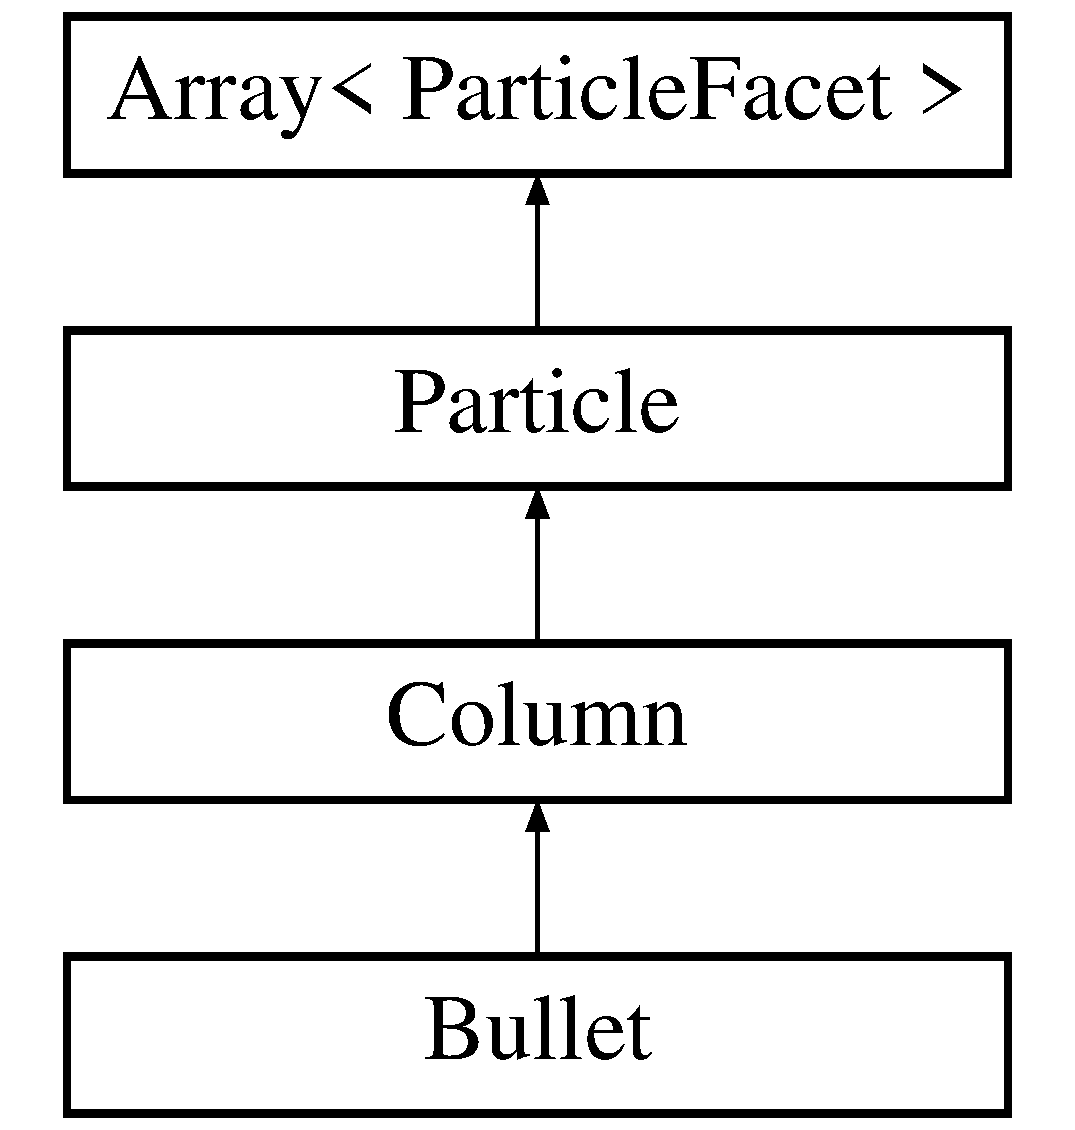
\includegraphics[height=4.000000cm]{class_bullet}
\end{center}
\end{figure}
\subsection*{Public Member Functions}
\begin{DoxyCompactItemize}
\item 
\mbox{\Hypertarget{class_bullet_a5bcdbed105749412de2da8f7ed0331fa}\label{class_bullet_a5bcdbed105749412de2da8f7ed0331fa}} 
{\bfseries Bullet} (const \mbox{\hyperlink{classcomplex}{complex}} \&refr\+Index, const \mbox{\hyperlink{struct_size}{Size}} \&size, double peak\+Height)
\end{DoxyCompactItemize}
\subsection*{Protected Member Functions}
\begin{DoxyCompactItemize}
\item 
\mbox{\Hypertarget{class_bullet_a5a6567716e528cebd8718dd728f5f85c}\label{class_bullet_a5a6567716e528cebd8718dd728f5f85c}} 
void {\bfseries Set\+Facet\+Params} () override
\end{DoxyCompactItemize}
\subsection*{Additional Inherited Members}


The documentation for this class was generated from the following files\+:\begin{DoxyCompactItemize}
\item 
particle/Bullet.\+h\item 
particle/Bullet.\+cpp\end{DoxyCompactItemize}

\hypertarget{class_bullet_rosette}{}\section{Bullet\+Rosette Class Reference}
\label{class_bullet_rosette}\index{Bullet\+Rosette@{Bullet\+Rosette}}


Inheritance diagram for Bullet\+Rosette\+:
% FIG 0


Collaboration diagram for Bullet\+Rosette\+:
% FIG 1
\subsection*{Public Member Functions}
\begin{DoxyCompactItemize}
\item 
\mbox{\Hypertarget{class_bullet_rosette_ad965a987a9247a0a3b3463b41d9856a9}\label{class_bullet_rosette_ad965a987a9247a0a3b3463b41d9856a9}} 
{\bfseries Bullet\+Rosette} (const \mbox{\hyperlink{classcomplex}{complex}} \&refr\+Index, const \mbox{\hyperlink{struct_size}{Size}} \&size, double peak\+Height)
\item 
\mbox{\Hypertarget{class_bullet_rosette_ae5b1763e464116c8429b8502d3cb07fa}\label{class_bullet_rosette_ae5b1763e464116c8429b8502d3cb07fa}} 
void {\bfseries Get\+Partical\+Facet\+Id\+Range} (\mbox{\hyperlink{class_facet}{Facet}} $\ast$facet, int \&begin, int \&end) const override
\end{DoxyCompactItemize}
\subsection*{Additional Inherited Members}


The documentation for this class was generated from the following files\+:\begin{DoxyCompactItemize}
\item 
particle/Bullet\+Rosette.\+h\item 
particle/Bullet\+Rosette.\+cpp\end{DoxyCompactItemize}

\hypertarget{class_calc_timer}{}\section{Calc\+Timer Class Reference}
\label{class_calc_timer}\index{Calc\+Timer@{Calc\+Timer}}
\subsection*{Public Member Functions}
\begin{DoxyCompactItemize}
\item 
\mbox{\Hypertarget{class_calc_timer_a072e9bf1de87302826a5de2cc36ed9a1}\label{class_calc_timer_a072e9bf1de87302826a5de2cc36ed9a1}} 
time\+\_\+t {\bfseries Start} ()
\item 
\mbox{\Hypertarget{class_calc_timer_a7026b92f345dbadd6341a57c4ca2b249}\label{class_calc_timer_a7026b92f345dbadd6341a57c4ca2b249}} 
time\+\_\+t {\bfseries Stop} ()
\item 
\mbox{\Hypertarget{class_calc_timer_a7d0990bf0484f8db9ab80bafedeedb17}\label{class_calc_timer_a7d0990bf0484f8db9ab80bafedeedb17}} 
long long {\bfseries Duration} ()
\item 
\mbox{\Hypertarget{class_calc_timer_aa50c249f66660b46c3ff8d86cc187129}\label{class_calc_timer_aa50c249f66660b46c3ff8d86cc187129}} 
void {\bfseries Left} (const long long \&ms)
\item 
\mbox{\Hypertarget{class_calc_timer_a7872ff0b769d29b8eff336bc4d279756}\label{class_calc_timer_a7872ff0b769d29b8eff336bc4d279756}} 
const std\+::time\+\_\+t \& {\bfseries End} (const long long \&ms)
\item 
\mbox{\Hypertarget{class_calc_timer_a31d046aca4d4d51fccbb2e53294f441a}\label{class_calc_timer_a31d046aca4d4d51fccbb2e53294f441a}} 
time\+\_\+t {\bfseries Begin} () const
\item 
\mbox{\Hypertarget{class_calc_timer_ae5ee06875f8d998eada9cc4e207f0563}\label{class_calc_timer_ae5ee06875f8d998eada9cc4e207f0563}} 
void {\bfseries Reset} ()
\item 
\mbox{\Hypertarget{class_calc_timer_a6b7db67583f793503861e71ea003f7e0}\label{class_calc_timer_a6b7db67583f793503861e71ea003f7e0}} 
std\+::string {\bfseries To\+String} ()
\item 
\mbox{\Hypertarget{class_calc_timer_a0e86da382dd944e9a94ea7497eeee24d}\label{class_calc_timer_a0e86da382dd944e9a94ea7497eeee24d}} 
std\+::string {\bfseries Elapsed} ()
\end{DoxyCompactItemize}


The documentation for this class was generated from the following files\+:\begin{DoxyCompactItemize}
\item 
common/Calc\+Timer.\+h\item 
common/Calc\+Timer.\+cpp\end{DoxyCompactItemize}

\hypertarget{class_certain_aggregate}{}\section{Certain\+Aggregate Class Reference}
\label{class_certain_aggregate}\index{Certain\+Aggregate@{Certain\+Aggregate}}


Inheritance diagram for Certain\+Aggregate\+:
% FIG 0


Collaboration diagram for Certain\+Aggregate\+:
% FIG 1
\subsection*{Public Member Functions}
\begin{DoxyCompactItemize}
\item 
\mbox{\Hypertarget{class_certain_aggregate_a8f2bd1d6a7c1f20e937ff8f0e42dc7c7}\label{class_certain_aggregate_a8f2bd1d6a7c1f20e937ff8f0e42dc7c7}} 
{\bfseries Certain\+Aggregate} (const \mbox{\hyperlink{classcomplex}{complex}} \&refr\+Index, double size\+Index)
\item 
\mbox{\Hypertarget{class_certain_aggregate_a9278fd4dd43852adc4e400fa4be6316e}\label{class_certain_aggregate_a9278fd4dd43852adc4e400fa4be6316e}} 
void {\bfseries Get\+Partical\+Facet\+Id\+Range} (\mbox{\hyperlink{class_facet}{Facet}} $\ast$facet, int \&begin, int \&end) const override
\end{DoxyCompactItemize}
\subsection*{Protected Member Functions}
\begin{DoxyCompactItemize}
\item 
\mbox{\Hypertarget{class_certain_aggregate_aa67b3812d8a84ad79bbcef90ac6bbe00}\label{class_certain_aggregate_aa67b3812d8a84ad79bbcef90ac6bbe00}} 
void {\bfseries Set\+Facet\+Params} () override
\end{DoxyCompactItemize}
\subsection*{Additional Inherited Members}


The documentation for this class was generated from the following files\+:\begin{DoxyCompactItemize}
\item 
particle/Certain\+Aggregate.\+h\item 
particle/Certain\+Aggregate.\+cpp\end{DoxyCompactItemize}

\hypertarget{class_clipper_lib_1_1_clipper}{}\section{Clipper\+Lib\+:\+:Clipper Class Reference}
\label{class_clipper_lib_1_1_clipper}\index{Clipper\+Lib\+::\+Clipper@{Clipper\+Lib\+::\+Clipper}}
Inheritance diagram for Clipper\+Lib\+:\+:Clipper\+:\begin{figure}[H]
\begin{center}
\leavevmode
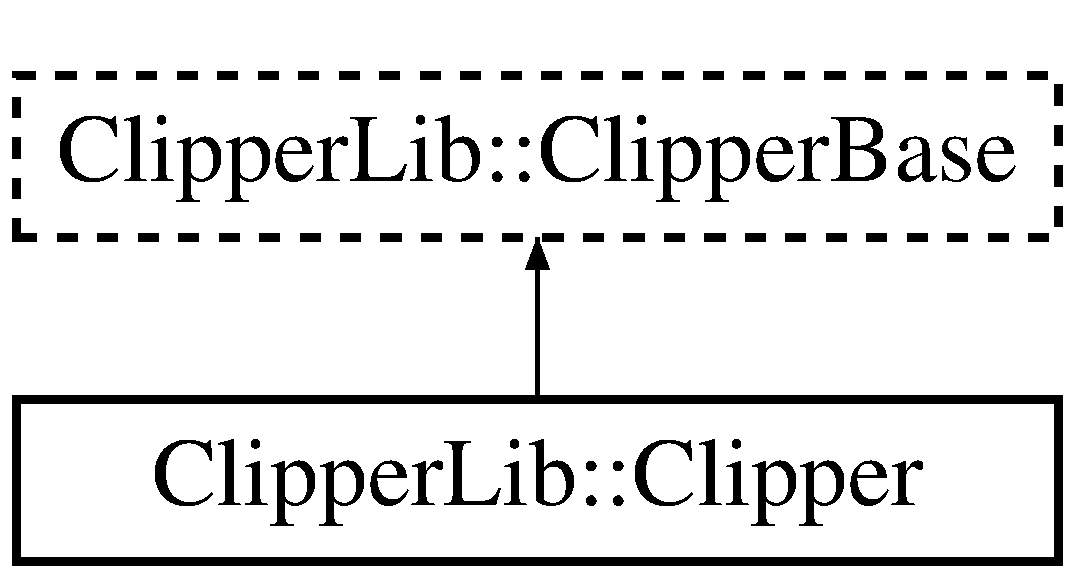
\includegraphics[height=2.000000cm]{class_clipper_lib_1_1_clipper}
\end{center}
\end{figure}
\subsection*{Public Member Functions}
\begin{DoxyCompactItemize}
\item 
\mbox{\Hypertarget{class_clipper_lib_1_1_clipper_adceb8536f6a80e8f115213dba9208427}\label{class_clipper_lib_1_1_clipper_adceb8536f6a80e8f115213dba9208427}} 
{\bfseries Clipper} (int init\+Options=0)
\item 
\mbox{\Hypertarget{class_clipper_lib_1_1_clipper_a06da196a4b4151edd2e5426ed48744cf}\label{class_clipper_lib_1_1_clipper_a06da196a4b4151edd2e5426ed48744cf}} 
bool {\bfseries Execute} (Clip\+Type clip\+Type, Paths \&solution, Poly\+Fill\+Type subj\+Fill\+Type=pft\+Even\+Odd, Poly\+Fill\+Type clip\+Fill\+Type=pft\+Even\+Odd)
\item 
\mbox{\Hypertarget{class_clipper_lib_1_1_clipper_aceb19a1e5a5c9e31067f4d1177793403}\label{class_clipper_lib_1_1_clipper_aceb19a1e5a5c9e31067f4d1177793403}} 
bool {\bfseries Execute} (Clip\+Type clip\+Type, \mbox{\hyperlink{class_clipper_lib_1_1_poly_tree}{Poly\+Tree}} \&polytree, Poly\+Fill\+Type subj\+Fill\+Type=pft\+Even\+Odd, Poly\+Fill\+Type clip\+Fill\+Type=pft\+Even\+Odd)
\item 
\mbox{\Hypertarget{class_clipper_lib_1_1_clipper_ad556ba9961f498de02d55dc95bc5a889}\label{class_clipper_lib_1_1_clipper_ad556ba9961f498de02d55dc95bc5a889}} 
bool {\bfseries Reverse\+Solution} ()
\item 
\mbox{\Hypertarget{class_clipper_lib_1_1_clipper_a44afc0c82a1d2607829b5fd21f7644ef}\label{class_clipper_lib_1_1_clipper_a44afc0c82a1d2607829b5fd21f7644ef}} 
void {\bfseries Reverse\+Solution} (bool value)
\item 
\mbox{\Hypertarget{class_clipper_lib_1_1_clipper_a50eb4c514466ed37fd365769e0bcf67b}\label{class_clipper_lib_1_1_clipper_a50eb4c514466ed37fd365769e0bcf67b}} 
bool {\bfseries Strictly\+Simple} ()
\item 
\mbox{\Hypertarget{class_clipper_lib_1_1_clipper_a85aa82d75e0d7d1f380d2e96231d6aa3}\label{class_clipper_lib_1_1_clipper_a85aa82d75e0d7d1f380d2e96231d6aa3}} 
void {\bfseries Strictly\+Simple} (bool value)
\item 
\mbox{\Hypertarget{class_clipper_lib_1_1_clipper_a6c09c403358ae8c4a190c2c3529aa01c}\label{class_clipper_lib_1_1_clipper_a6c09c403358ae8c4a190c2c3529aa01c}} 
void {\bfseries Z\+Fill\+Function} (Z\+Fill\+Callback z\+Fill\+Func)
\end{DoxyCompactItemize}
\subsection*{Protected Member Functions}
\begin{DoxyCompactItemize}
\item 
\mbox{\Hypertarget{class_clipper_lib_1_1_clipper_a14c704b062e8a079e34a8ce40838861e}\label{class_clipper_lib_1_1_clipper_a14c704b062e8a079e34a8ce40838861e}} 
void {\bfseries Reset} ()
\item 
\mbox{\Hypertarget{class_clipper_lib_1_1_clipper_a3e8757e5f8a6ffcb7fd0f9630fde02d3}\label{class_clipper_lib_1_1_clipper_a3e8757e5f8a6ffcb7fd0f9630fde02d3}} 
virtual bool {\bfseries Execute\+Internal} ()
\end{DoxyCompactItemize}
\subsection*{Additional Inherited Members}


The documentation for this class was generated from the following files\+:\begin{DoxyCompactItemize}
\item 
geometry/clipper/clipper.\+hpp\item 
geometry/clipper/clipper.\+cpp\end{DoxyCompactItemize}

\hypertarget{class_clipper_lib_1_1_clipper_base}{}\section{Clipper\+Lib\+:\+:Clipper\+Base Class Reference}
\label{class_clipper_lib_1_1_clipper_base}\index{Clipper\+Lib\+::\+Clipper\+Base@{Clipper\+Lib\+::\+Clipper\+Base}}
Inheritance diagram for Clipper\+Lib\+:\+:Clipper\+Base\+:\begin{figure}[H]
\begin{center}
\leavevmode
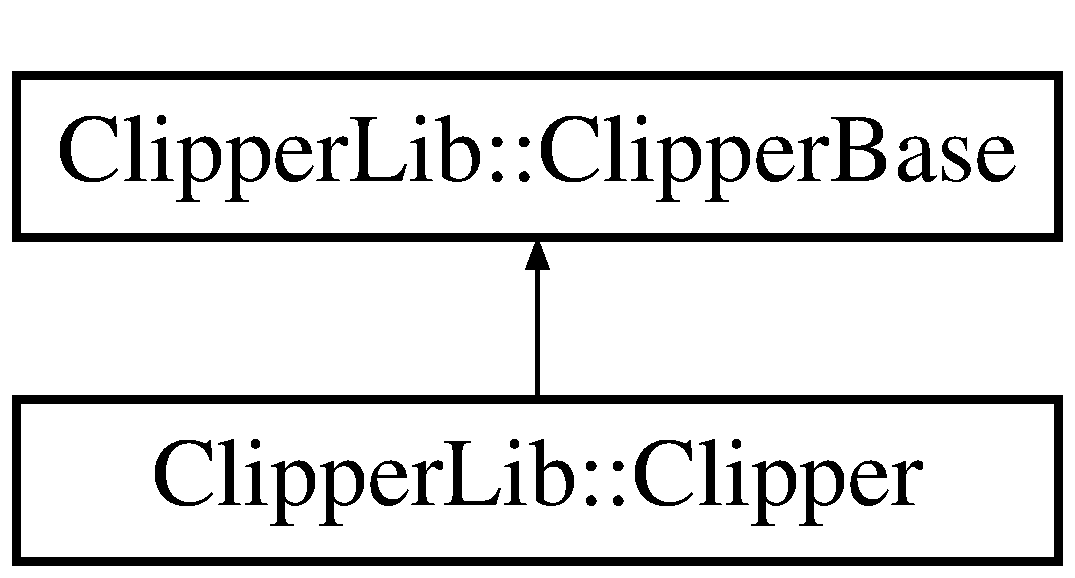
\includegraphics[height=2.000000cm]{class_clipper_lib_1_1_clipper_base}
\end{center}
\end{figure}
\subsection*{Public Member Functions}
\begin{DoxyCompactItemize}
\item 
\mbox{\Hypertarget{class_clipper_lib_1_1_clipper_base_a7545ac6e146894dc8416887eadd01dba}\label{class_clipper_lib_1_1_clipper_base_a7545ac6e146894dc8416887eadd01dba}} 
bool {\bfseries Add\+Path} (const Path \&pg, Poly\+Type Poly\+Typ, bool Closed)
\item 
\mbox{\Hypertarget{class_clipper_lib_1_1_clipper_base_a2395967b47fb9f3f5846e2bf56c18f67}\label{class_clipper_lib_1_1_clipper_base_a2395967b47fb9f3f5846e2bf56c18f67}} 
bool {\bfseries Add\+Paths} (const Paths \&ppg, Poly\+Type Poly\+Typ, bool Closed)
\item 
\mbox{\Hypertarget{class_clipper_lib_1_1_clipper_base_a5690952fe8c2cb047025566405827821}\label{class_clipper_lib_1_1_clipper_base_a5690952fe8c2cb047025566405827821}} 
virtual void {\bfseries Clear} ()
\item 
\mbox{\Hypertarget{class_clipper_lib_1_1_clipper_base_a5590a5454248ac3f6beeba7f9690f62e}\label{class_clipper_lib_1_1_clipper_base_a5590a5454248ac3f6beeba7f9690f62e}} 
\mbox{\hyperlink{struct_clipper_lib_1_1_int_rect}{Int\+Rect}} {\bfseries Get\+Bounds} ()
\item 
\mbox{\Hypertarget{class_clipper_lib_1_1_clipper_base_a95c47199aeb139b13059968bc6056f44}\label{class_clipper_lib_1_1_clipper_base_a95c47199aeb139b13059968bc6056f44}} 
bool {\bfseries Preserve\+Collinear} ()
\item 
\mbox{\Hypertarget{class_clipper_lib_1_1_clipper_base_aa827cfffd9be40dba7d503a3da708b91}\label{class_clipper_lib_1_1_clipper_base_aa827cfffd9be40dba7d503a3da708b91}} 
void {\bfseries Preserve\+Collinear} (bool value)
\end{DoxyCompactItemize}
\subsection*{Protected Types}
\begin{DoxyCompactItemize}
\item 
\mbox{\Hypertarget{class_clipper_lib_1_1_clipper_base_addb22572066d3983dcd5797c542df00b}\label{class_clipper_lib_1_1_clipper_base_addb22572066d3983dcd5797c542df00b}} 
typedef std\+::vector$<$ \mbox{\hyperlink{struct_clipper_lib_1_1_local_minimum}{Local\+Minimum}} $>$ {\bfseries Minima\+List}
\end{DoxyCompactItemize}
\subsection*{Protected Member Functions}
\begin{DoxyCompactItemize}
\item 
\mbox{\Hypertarget{class_clipper_lib_1_1_clipper_base_a311dbbec1454ab7965e363a0359f5ee4}\label{class_clipper_lib_1_1_clipper_base_a311dbbec1454ab7965e363a0359f5ee4}} 
void {\bfseries Dispose\+Local\+Minima\+List} ()
\item 
\mbox{\Hypertarget{class_clipper_lib_1_1_clipper_base_a906ea17c9dc8822d689e54c3243e7f58}\label{class_clipper_lib_1_1_clipper_base_a906ea17c9dc8822d689e54c3243e7f58}} 
\mbox{\hyperlink{struct_clipper_lib_1_1_t_edge}{T\+Edge}} $\ast$ {\bfseries Add\+Bounds\+To\+L\+ML} (\mbox{\hyperlink{struct_clipper_lib_1_1_t_edge}{T\+Edge}} $\ast$e, bool Is\+Closed)
\item 
\mbox{\Hypertarget{class_clipper_lib_1_1_clipper_base_a9554e9f2273c39e0f5f07d3cd73533e6}\label{class_clipper_lib_1_1_clipper_base_a9554e9f2273c39e0f5f07d3cd73533e6}} 
void {\bfseries Pop\+Local\+Minima} ()
\item 
\mbox{\Hypertarget{class_clipper_lib_1_1_clipper_base_a125febb065f23fc55dafffe8d185b642}\label{class_clipper_lib_1_1_clipper_base_a125febb065f23fc55dafffe8d185b642}} 
virtual void {\bfseries Reset} ()
\item 
\mbox{\Hypertarget{class_clipper_lib_1_1_clipper_base_a292655c74a7e70a8b8829337c632bdf0}\label{class_clipper_lib_1_1_clipper_base_a292655c74a7e70a8b8829337c632bdf0}} 
\mbox{\hyperlink{struct_clipper_lib_1_1_t_edge}{T\+Edge}} $\ast$ {\bfseries Process\+Bound} (\mbox{\hyperlink{struct_clipper_lib_1_1_t_edge}{T\+Edge}} $\ast$E, bool Is\+Clockwise)
\item 
\mbox{\Hypertarget{class_clipper_lib_1_1_clipper_base_ae57efb542cfbbc42d000815e8a2e2877}\label{class_clipper_lib_1_1_clipper_base_ae57efb542cfbbc42d000815e8a2e2877}} 
void {\bfseries Do\+Minima\+L\+ML} (\mbox{\hyperlink{struct_clipper_lib_1_1_t_edge}{T\+Edge}} $\ast$E1, \mbox{\hyperlink{struct_clipper_lib_1_1_t_edge}{T\+Edge}} $\ast$E2, bool Is\+Closed)
\item 
\mbox{\Hypertarget{class_clipper_lib_1_1_clipper_base_a13086e8d650edc1a024813d3a8469120}\label{class_clipper_lib_1_1_clipper_base_a13086e8d650edc1a024813d3a8469120}} 
\mbox{\hyperlink{struct_clipper_lib_1_1_t_edge}{T\+Edge}} $\ast$ {\bfseries Descend\+To\+Min} (\mbox{\hyperlink{struct_clipper_lib_1_1_t_edge}{T\+Edge}} $\ast$\&E)
\item 
\mbox{\Hypertarget{class_clipper_lib_1_1_clipper_base_afafbf0dafffb5ad6f5a5c30dbed6378f}\label{class_clipper_lib_1_1_clipper_base_afafbf0dafffb5ad6f5a5c30dbed6378f}} 
void {\bfseries Ascend\+To\+Max} (\mbox{\hyperlink{struct_clipper_lib_1_1_t_edge}{T\+Edge}} $\ast$\&E, bool Appending, bool Is\+Closed)
\end{DoxyCompactItemize}
\subsection*{Protected Attributes}
\begin{DoxyCompactItemize}
\item 
\mbox{\Hypertarget{class_clipper_lib_1_1_clipper_base_ab6ed40f62810c0f894878c79d74afb36}\label{class_clipper_lib_1_1_clipper_base_ab6ed40f62810c0f894878c79d74afb36}} 
Minima\+List\+::iterator {\bfseries m\+\_\+\+Current\+LM}
\item 
\mbox{\Hypertarget{class_clipper_lib_1_1_clipper_base_a970749dc12a20e980c932af040f8a8c5}\label{class_clipper_lib_1_1_clipper_base_a970749dc12a20e980c932af040f8a8c5}} 
Minima\+List {\bfseries m\+\_\+\+Minima\+List}
\item 
\mbox{\Hypertarget{class_clipper_lib_1_1_clipper_base_aea11d183617adc12d7ba2b84533f7f45}\label{class_clipper_lib_1_1_clipper_base_aea11d183617adc12d7ba2b84533f7f45}} 
bool {\bfseries m\+\_\+\+Use\+Full\+Range}
\item 
\mbox{\Hypertarget{class_clipper_lib_1_1_clipper_base_a8bfc007c0c0afd4e9d252dac0ef5daa0}\label{class_clipper_lib_1_1_clipper_base_a8bfc007c0c0afd4e9d252dac0ef5daa0}} 
Edge\+List {\bfseries m\+\_\+edges}
\item 
\mbox{\Hypertarget{class_clipper_lib_1_1_clipper_base_aad4ca0f2a16a6fb466036b36cc5ff638}\label{class_clipper_lib_1_1_clipper_base_aad4ca0f2a16a6fb466036b36cc5ff638}} 
bool {\bfseries m\+\_\+\+Preserve\+Collinear}
\item 
\mbox{\Hypertarget{class_clipper_lib_1_1_clipper_base_aa2508f5b2a599294c359271506441fbd}\label{class_clipper_lib_1_1_clipper_base_aa2508f5b2a599294c359271506441fbd}} 
bool {\bfseries m\+\_\+\+Has\+Open\+Paths}
\end{DoxyCompactItemize}


The documentation for this class was generated from the following files\+:\begin{DoxyCompactItemize}
\item 
geometry/clipper/clipper.\+hpp\item 
geometry/clipper/clipper.\+cpp\end{DoxyCompactItemize}

\hypertarget{class_clipper_lib_1_1clipper_exception}{}\section{Clipper\+Lib\+:\+:clipper\+Exception Class Reference}
\label{class_clipper_lib_1_1clipper_exception}\index{Clipper\+Lib\+::clipper\+Exception@{Clipper\+Lib\+::clipper\+Exception}}
Inheritance diagram for Clipper\+Lib\+:\+:clipper\+Exception\+:\begin{figure}[H]
\begin{center}
\leavevmode
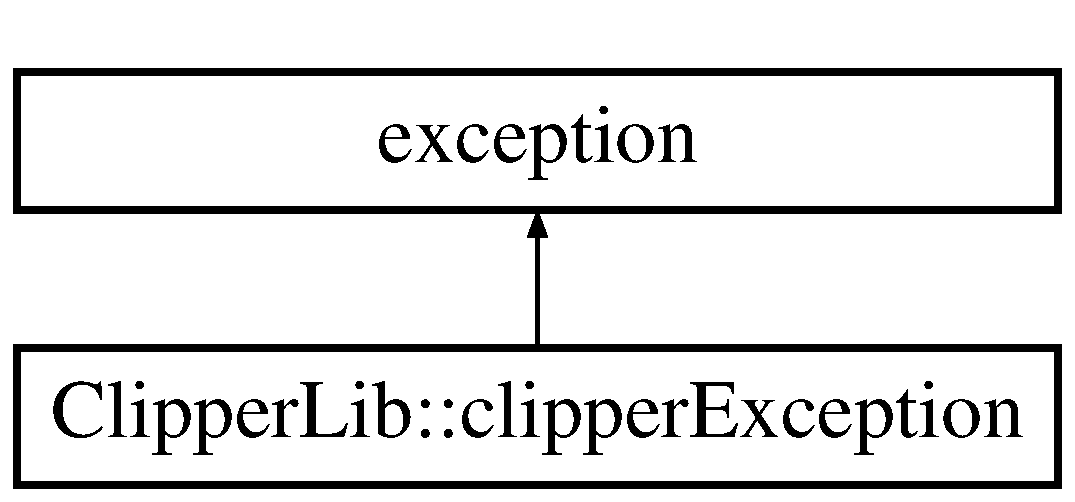
\includegraphics[height=2.000000cm]{class_clipper_lib_1_1clipper_exception}
\end{center}
\end{figure}
\subsection*{Public Member Functions}
\begin{DoxyCompactItemize}
\item 
\mbox{\Hypertarget{class_clipper_lib_1_1clipper_exception_a7d44b32d06cd870500355667f6e0d6ed}\label{class_clipper_lib_1_1clipper_exception_a7d44b32d06cd870500355667f6e0d6ed}} 
{\bfseries clipper\+Exception} (const char $\ast$description)
\item 
\mbox{\Hypertarget{class_clipper_lib_1_1clipper_exception_a32b7ac5a3176d9040ef0a863fd54657a}\label{class_clipper_lib_1_1clipper_exception_a32b7ac5a3176d9040ef0a863fd54657a}} 
virtual const char $\ast$ {\bfseries what} () const  throw ()
\end{DoxyCompactItemize}


The documentation for this class was generated from the following file\+:\begin{DoxyCompactItemize}
\item 
geometry/clipper/clipper.\+hpp\end{DoxyCompactItemize}

\hypertarget{class_clipper_lib_1_1_clipper_offset}{}\section{Clipper\+Lib\+:\+:Clipper\+Offset Class Reference}
\label{class_clipper_lib_1_1_clipper_offset}\index{Clipper\+Lib\+::\+Clipper\+Offset@{Clipper\+Lib\+::\+Clipper\+Offset}}
\subsection*{Public Member Functions}
\begin{DoxyCompactItemize}
\item 
\mbox{\Hypertarget{class_clipper_lib_1_1_clipper_offset_a45b4750989901db0c3865c374abdfcdc}\label{class_clipper_lib_1_1_clipper_offset_a45b4750989901db0c3865c374abdfcdc}} 
{\bfseries Clipper\+Offset} (double miter\+Limit=2.\+0, double round\+Precision=0.\+25)
\item 
\mbox{\Hypertarget{class_clipper_lib_1_1_clipper_offset_a0cd68e3690072f510924a5b25291043b}\label{class_clipper_lib_1_1_clipper_offset_a0cd68e3690072f510924a5b25291043b}} 
void {\bfseries Add\+Path} (const Path \&path, Join\+Type join\+Type, End\+Type end\+Type)
\item 
\mbox{\Hypertarget{class_clipper_lib_1_1_clipper_offset_a18b35198f6370d76885af995ee2f16cb}\label{class_clipper_lib_1_1_clipper_offset_a18b35198f6370d76885af995ee2f16cb}} 
void {\bfseries Add\+Paths} (const Paths \&paths, Join\+Type join\+Type, End\+Type end\+Type)
\item 
\mbox{\Hypertarget{class_clipper_lib_1_1_clipper_offset_ac591b25e483a52c99c3190a256ad4589}\label{class_clipper_lib_1_1_clipper_offset_ac591b25e483a52c99c3190a256ad4589}} 
void {\bfseries Execute} (Paths \&solution, double delta)
\item 
\mbox{\Hypertarget{class_clipper_lib_1_1_clipper_offset_a3aaa9fcc20e503c967a23f1793536118}\label{class_clipper_lib_1_1_clipper_offset_a3aaa9fcc20e503c967a23f1793536118}} 
void {\bfseries Execute} (\mbox{\hyperlink{class_clipper_lib_1_1_poly_tree}{Poly\+Tree}} \&solution, double delta)
\item 
\mbox{\Hypertarget{class_clipper_lib_1_1_clipper_offset_ab444433587b6a3f6c89655938d889c7d}\label{class_clipper_lib_1_1_clipper_offset_ab444433587b6a3f6c89655938d889c7d}} 
void {\bfseries Clear} ()
\end{DoxyCompactItemize}
\subsection*{Public Attributes}
\begin{DoxyCompactItemize}
\item 
\mbox{\Hypertarget{class_clipper_lib_1_1_clipper_offset_a36b3bf4571e5b831edd584cbcb179246}\label{class_clipper_lib_1_1_clipper_offset_a36b3bf4571e5b831edd584cbcb179246}} 
double {\bfseries Miter\+Limit}
\item 
\mbox{\Hypertarget{class_clipper_lib_1_1_clipper_offset_a6c1735720b06e6b92dc25891014b2a92}\label{class_clipper_lib_1_1_clipper_offset_a6c1735720b06e6b92dc25891014b2a92}} 
double {\bfseries Arc\+Tolerance}
\end{DoxyCompactItemize}


The documentation for this class was generated from the following files\+:\begin{DoxyCompactItemize}
\item 
geometry/clipper/clipper.\+hpp\item 
geometry/clipper/clipper.\+cpp\end{DoxyCompactItemize}

\hypertarget{class_column}{}\section{Column Class Reference}
\label{class_column}\index{Column@{Column}}


The \mbox{\hyperlink{class_column}{Column}} class.  




{\ttfamily \#include $<$Column.\+h$>$}



Inheritance diagram for Column\+:
% FIG 0


Collaboration diagram for Column\+:
% FIG 1
\subsection*{Public Member Functions}
\begin{DoxyCompactItemize}
\item 
\mbox{\Hypertarget{class_column_a7eaee92cd3aed5562652242037e8a58c}\label{class_column_a7eaee92cd3aed5562652242037e8a58c}} 
{\bfseries Column} (int n\+Facets, const \mbox{\hyperlink{classcomplex}{complex}} \&refr\+Index, const \mbox{\hyperlink{struct_size}{Size}} \&size, bool is\+Non\+Convex)
\end{DoxyCompactItemize}
\subsection*{Protected Member Functions}
\begin{DoxyCompactItemize}
\item 
\mbox{\Hypertarget{class_column_a6c1b221d3b77b84dc327080bdc832dc8}\label{class_column_a6c1b221d3b77b84dc327080bdc832dc8}} 
void {\bfseries Set\+Facet\+Params} () override
\item 
\mbox{\Hypertarget{class_column_af9e69ceebb96af7c4968e51cdcf7f01a}\label{class_column_af9e69ceebb96af7c4968e51cdcf7f01a}} 
void {\bfseries Set\+Bases} (\mbox{\hyperlink{class_facet}{Facet}} \&top, \mbox{\hyperlink{class_facet}{Facet}} \&bottom)
\item 
\mbox{\Hypertarget{class_column_ac0558dde864e35ac694a4463a0cadb99}\label{class_column_ac0558dde864e35ac694a4463a0cadb99}} 
void {\bfseries Set\+Two\+Diagonal\+Points} (int index, \mbox{\hyperlink{struct_point3f}{Point3f}} $\ast$facet, double x, double y, double z)
\item 
\mbox{\Hypertarget{class_column_aa12a30383a19d408f4d57b9aa2b348a2}\label{class_column_aa12a30383a19d408f4d57b9aa2b348a2}} 
void {\bfseries Set\+Sides} (\mbox{\hyperlink{class_facet}{Facet}} \&base\+Top, \mbox{\hyperlink{class_facet}{Facet}} \&base\+Bottom)
\item 
\mbox{\Hypertarget{class_column_aaff3281532436d6c70c0eaca569665d8}\label{class_column_aaff3281532436d6c70c0eaca569665d8}} 
void {\bfseries Set\+Side\+Facet\+Params} (int first, int last)
\end{DoxyCompactItemize}
\subsection*{Protected Attributes}
\begin{DoxyCompactItemize}
\item 
\mbox{\Hypertarget{class_column_aad02a5a2b9c19658759d57d399e84ce4}\label{class_column_aad02a5a2b9c19658759d57d399e84ce4}} 
\mbox{\hyperlink{class_couple}{Couple}}$<$ int $>$ {\bfseries m\+\_\+side\+Facet\+I\+Ds}
\item 
\mbox{\Hypertarget{class_column_a6d4ce98d9797d37ce75073ab9853e218}\label{class_column_a6d4ce98d9797d37ce75073ab9853e218}} 
\mbox{\hyperlink{struct_size}{Size}} {\bfseries m\+\_\+size}
\end{DoxyCompactItemize}
\subsection*{Static Protected Attributes}
\begin{DoxyCompactItemize}
\item 
\mbox{\Hypertarget{class_column_a5988fac458953d180b4dcb1a5d2826fa}\label{class_column_a5988fac458953d180b4dcb1a5d2826fa}} 
static const int \mbox{\hyperlink{class_column_a5988fac458953d180b4dcb1a5d2826fa}{B\+A\+S\+E\+\_\+\+N\+UM}} = 2
\begin{DoxyCompactList}\small\item\em number of bases \end{DoxyCompactList}\item 
\mbox{\Hypertarget{class_column_aa3e3e5d6543b7e34191914ecdd7368bd}\label{class_column_aa3e3e5d6543b7e34191914ecdd7368bd}} 
static const int \mbox{\hyperlink{class_column_aa3e3e5d6543b7e34191914ecdd7368bd}{S\+I\+D\+E\+\_\+\+V\+E\+R\+T\+E\+X\+\_\+\+N\+UM}} = 4
\begin{DoxyCompactList}\small\item\em number of vertex of the each side facet \end{DoxyCompactList}\item 
\mbox{\Hypertarget{class_column_a54b8114ca0318ba212dfe2bda99e0918}\label{class_column_a54b8114ca0318ba212dfe2bda99e0918}} 
static const int \mbox{\hyperlink{class_column_a54b8114ca0318ba212dfe2bda99e0918}{B\+A\+S\+E\+\_\+\+V\+E\+R\+T\+E\+X\+\_\+\+N\+UM}} = 6
\begin{DoxyCompactList}\small\item\em number of side facets \end{DoxyCompactList}\end{DoxyCompactItemize}
\subsection*{Additional Inherited Members}


\subsection{Detailed Description}
The \mbox{\hyperlink{class_column}{Column}} class. 

The documentation for this class was generated from the following files\+:\begin{DoxyCompactItemize}
\item 
particle/Column.\+h\item 
particle/Column.\+cpp\end{DoxyCompactItemize}

\hypertarget{class_complete_reflection_incidence}{}\section{Complete\+Reflection\+Incidence Class Reference}
\label{class_complete_reflection_incidence}\index{Complete\+Reflection\+Incidence@{Complete\+Reflection\+Incidence}}


Inheritance diagram for Complete\+Reflection\+Incidence\+:
% FIG 0


Collaboration diagram for Complete\+Reflection\+Incidence\+:
% FIG 1
\subsection*{Public Member Functions}
\begin{DoxyCompactItemize}
\item 
\mbox{\Hypertarget{class_complete_reflection_incidence_a3364068e607c73d4a215c3ccd9a5e854}\label{class_complete_reflection_incidence_a3364068e607c73d4a215c3ccd9a5e854}} 
virtual void {\bfseries Compute\+Directions} (\mbox{\hyperlink{class_beam}{Beam}} \&beam, \mbox{\hyperlink{class_splitting}{Splitting}} \&splitter) const override
\item 
\mbox{\Hypertarget{class_complete_reflection_incidence_a8e719e4c8dd8ced7fcf8070f5117fb96}\label{class_complete_reflection_incidence_a8e719e4c8dd8ced7fcf8070f5117fb96}} 
virtual void {\bfseries Compute\+Jones\+Matrices} (\mbox{\hyperlink{class_beam}{Beam}} \&beam, \mbox{\hyperlink{class_splitting}{Splitting}} \&splitter) const override
\item 
\mbox{\Hypertarget{class_complete_reflection_incidence_a36f51c084d4aefecdb224ac0b791a552}\label{class_complete_reflection_incidence_a36f51c084d4aefecdb224ac0b791a552}} 
void {\bfseries Compute\+Optical\+Paths} (const \mbox{\hyperlink{class_beam}{Beam}} \&incident\+Beam, \mbox{\hyperlink{class_splitting}{Splitting}} \&splitter) const
\end{DoxyCompactItemize}


The documentation for this class was generated from the following files\+:\begin{DoxyCompactItemize}
\item 
incidence/Complete\+Reflection\+Incidence.\+h\item 
incidence/Complete\+Reflection\+Incidence.\+cpp\end{DoxyCompactItemize}

\hypertarget{classcomplex}{}\section{complex Class Reference}
\label{classcomplex}\index{complex@{complex}}


This class provides a complex numbers and operation with them.  




{\ttfamily \#include $<$compl.\+hpp$>$}

\subsection*{Public Member Functions}
\begin{DoxyCompactItemize}
\item 
\mbox{\Hypertarget{classcomplex_a02480dc4c97bb508d44fd2a9218110b9}\label{classcomplex_a02480dc4c97bb508d44fd2a9218110b9}} 
{\bfseries complex} (double r=0, double i=0)
\item 
\mbox{\Hypertarget{classcomplex_a87c671cba1258ebf806685ee048c04e4}\label{classcomplex_a87c671cba1258ebf806685ee048c04e4}} 
\mbox{\hyperlink{classcomplex}{complex}} \& {\bfseries operator=} (const \mbox{\hyperlink{classcomplex}{complex}} \&b)
\item 
\mbox{\Hypertarget{classcomplex_a5782c9c6c5d00e553e859605fedb3aca}\label{classcomplex_a5782c9c6c5d00e553e859605fedb3aca}} 
\mbox{\hyperlink{classcomplex}{complex}} {\bfseries operator+} () const
\item 
\mbox{\Hypertarget{classcomplex_ac087cdc8ef2c4851ac7a959f33789474}\label{classcomplex_ac087cdc8ef2c4851ac7a959f33789474}} 
\mbox{\hyperlink{classcomplex}{complex}} {\bfseries operator+} (double x) const
\item 
\mbox{\Hypertarget{classcomplex_a635bb2d03c023671ac1b742aaec06c03}\label{classcomplex_a635bb2d03c023671ac1b742aaec06c03}} 
\mbox{\hyperlink{classcomplex}{complex}} {\bfseries operator+} (const \mbox{\hyperlink{classcomplex}{complex}} \&z) const
\item 
\mbox{\Hypertarget{classcomplex_a69a3baf8f78d9798c2aa220d03a53077}\label{classcomplex_a69a3baf8f78d9798c2aa220d03a53077}} 
\mbox{\hyperlink{classcomplex}{complex}} {\bfseries operator+=} (const \mbox{\hyperlink{classcomplex}{complex}} \&z)
\item 
\mbox{\Hypertarget{classcomplex_ad6f6fa4a782cd727756f8b8d7b61bc21}\label{classcomplex_ad6f6fa4a782cd727756f8b8d7b61bc21}} 
\mbox{\hyperlink{classcomplex}{complex}} {\bfseries operator+=} (double x)
\item 
\mbox{\Hypertarget{classcomplex_a969988c8e6c2a3af52c64e531471f6c0}\label{classcomplex_a969988c8e6c2a3af52c64e531471f6c0}} 
\mbox{\hyperlink{classcomplex}{complex}} {\bfseries operator-\/} () const
\item 
\mbox{\Hypertarget{classcomplex_a49b901ecd286980d823050c2116efd1d}\label{classcomplex_a49b901ecd286980d823050c2116efd1d}} 
\mbox{\hyperlink{classcomplex}{complex}} {\bfseries operator-\/} (double x) const
\item 
\mbox{\Hypertarget{classcomplex_a88bd18ff6c84dec46c8a982a6b9ca60c}\label{classcomplex_a88bd18ff6c84dec46c8a982a6b9ca60c}} 
\mbox{\hyperlink{classcomplex}{complex}} {\bfseries operator-\/} (const \mbox{\hyperlink{classcomplex}{complex}} \&z) const
\item 
\mbox{\Hypertarget{classcomplex_a746573fc41a6012f115e1c38b37ea591}\label{classcomplex_a746573fc41a6012f115e1c38b37ea591}} 
\mbox{\hyperlink{classcomplex}{complex}} {\bfseries operator-\/=} (const \mbox{\hyperlink{classcomplex}{complex}} \&z)
\item 
\mbox{\Hypertarget{classcomplex_a18b50305c069b3cf18cb8709af54cce3}\label{classcomplex_a18b50305c069b3cf18cb8709af54cce3}} 
\mbox{\hyperlink{classcomplex}{complex}} {\bfseries operator-\/=} (double x)
\item 
\mbox{\Hypertarget{classcomplex_aa1a174e630f6affcaf6910824732bf29}\label{classcomplex_aa1a174e630f6affcaf6910824732bf29}} 
\mbox{\hyperlink{classcomplex}{complex}} {\bfseries operator$\ast$} (double x) const
\item 
\mbox{\Hypertarget{classcomplex_a3b067d7031334b4544bacfbadf198f30}\label{classcomplex_a3b067d7031334b4544bacfbadf198f30}} 
\mbox{\hyperlink{classcomplex}{complex}} {\bfseries operator$\ast$} (const \mbox{\hyperlink{classcomplex}{complex}} \&z) const
\item 
\mbox{\Hypertarget{classcomplex_aaa9424e138835a4e727e12984899e68d}\label{classcomplex_aaa9424e138835a4e727e12984899e68d}} 
\mbox{\hyperlink{classcomplex}{complex}} {\bfseries operator$\ast$=} (const \mbox{\hyperlink{classcomplex}{complex}} \&z)
\item 
\mbox{\Hypertarget{classcomplex_a13aceba61621fa9df397e640355dbaf0}\label{classcomplex_a13aceba61621fa9df397e640355dbaf0}} 
\mbox{\hyperlink{classcomplex}{complex}} {\bfseries operator$\ast$=} (double x)
\item 
\mbox{\Hypertarget{classcomplex_a0ab4a3bb2f9742fda6aefcfb50ce6a3b}\label{classcomplex_a0ab4a3bb2f9742fda6aefcfb50ce6a3b}} 
\mbox{\hyperlink{classcomplex}{complex}} {\bfseries operator/} (double x) const
\item 
\mbox{\Hypertarget{classcomplex_a97dd0fdcf0fff662746feffbe450e058}\label{classcomplex_a97dd0fdcf0fff662746feffbe450e058}} 
\mbox{\hyperlink{classcomplex}{complex}} {\bfseries operator/} (const \mbox{\hyperlink{classcomplex}{complex}} \&z) const
\item 
\mbox{\Hypertarget{classcomplex_a25e80fe4a8c8306ee86eeb4f2e7e0e2d}\label{classcomplex_a25e80fe4a8c8306ee86eeb4f2e7e0e2d}} 
\mbox{\hyperlink{classcomplex}{complex}} {\bfseries operator/=} (double x)
\item 
\mbox{\Hypertarget{classcomplex_a9942c93796f014f0092285c6860c0245}\label{classcomplex_a9942c93796f014f0092285c6860c0245}} 
\mbox{\hyperlink{classcomplex}{complex}} {\bfseries operator/=} (const \mbox{\hyperlink{classcomplex}{complex}} \&z)
\item 
\mbox{\Hypertarget{classcomplex_ad6768b39295754d62e89bdc4ece6c2bd}\label{classcomplex_ad6768b39295754d62e89bdc4ece6c2bd}} 
bool {\bfseries operator==} (const \mbox{\hyperlink{classcomplex}{complex}} \&z) const
\item 
\mbox{\Hypertarget{classcomplex_a9803106eea35a7855b8b7315ff3e8143}\label{classcomplex_a9803106eea35a7855b8b7315ff3e8143}} 
bool {\bfseries operator!=} (const \mbox{\hyperlink{classcomplex}{complex}} \&z) const
\item 
\mbox{\Hypertarget{classcomplex_ac5dc3102b9192b10f9805ffd8482cf88}\label{classcomplex_ac5dc3102b9192b10f9805ffd8482cf88}} 
bool {\bfseries operator==} (double x) const
\item 
\mbox{\Hypertarget{classcomplex_ac88200bf9f846fb7e3682807a643bc3e}\label{classcomplex_ac88200bf9f846fb7e3682807a643bc3e}} 
bool {\bfseries operator!=} (double x) const
\end{DoxyCompactItemize}
\subsection*{Friends}
\begin{DoxyCompactItemize}
\item 
\mbox{\Hypertarget{classcomplex_a16cdb9ed1871116f72a2b64337dd396c}\label{classcomplex_a16cdb9ed1871116f72a2b64337dd396c}} 
\mbox{\hyperlink{classcomplex}{complex}} {\bfseries operator+} (double x, const \mbox{\hyperlink{classcomplex}{complex}} \&z)
\item 
\mbox{\Hypertarget{classcomplex_a1dfb39ebfca8156eacee00d4d0b36c4b}\label{classcomplex_a1dfb39ebfca8156eacee00d4d0b36c4b}} 
\mbox{\hyperlink{classcomplex}{complex}} {\bfseries operator-\/} (double x, const \mbox{\hyperlink{classcomplex}{complex}} \&z)
\item 
\mbox{\Hypertarget{classcomplex_aa0830a62ca6e2b1d6789caef36086d7b}\label{classcomplex_aa0830a62ca6e2b1d6789caef36086d7b}} 
\mbox{\hyperlink{classcomplex}{complex}} {\bfseries operator/} (double x, const \mbox{\hyperlink{classcomplex}{complex}} \&z)
\item 
\mbox{\Hypertarget{classcomplex_a10b8cb0eba7d2791c0f4de7d860f01d1}\label{classcomplex_a10b8cb0eba7d2791c0f4de7d860f01d1}} 
double \& {\bfseries real} (\mbox{\hyperlink{classcomplex}{complex}} \&z)
\item 
\mbox{\Hypertarget{classcomplex_a2ff31e9507e7dc48651b4e448ac98159}\label{classcomplex_a2ff31e9507e7dc48651b4e448ac98159}} 
double \& {\bfseries imag} (\mbox{\hyperlink{classcomplex}{complex}} \&z)
\item 
\mbox{\Hypertarget{classcomplex_a075dd12490d06326130b46dda0d616a8}\label{classcomplex_a075dd12490d06326130b46dda0d616a8}} 
double {\bfseries real} (const \mbox{\hyperlink{classcomplex}{complex}} \&z)
\item 
\mbox{\Hypertarget{classcomplex_a54e570e34b8ff9691500e8fd27955fdb}\label{classcomplex_a54e570e34b8ff9691500e8fd27955fdb}} 
double {\bfseries imag} (const \mbox{\hyperlink{classcomplex}{complex}} \&z)
\item 
\mbox{\Hypertarget{classcomplex_adcb2904dc1b01d5ed3a9b6b3bd135d9b}\label{classcomplex_adcb2904dc1b01d5ed3a9b6b3bd135d9b}} 
double {\bfseries norm} (const \mbox{\hyperlink{classcomplex}{complex}} \&z)
\item 
\mbox{\Hypertarget{classcomplex_ac4eba7c0a4012bfc017abe67291dace1}\label{classcomplex_ac4eba7c0a4012bfc017abe67291dace1}} 
\mbox{\hyperlink{classcomplex}{complex}} {\bfseries conj} (const \mbox{\hyperlink{classcomplex}{complex}} \&z)
\item 
\mbox{\Hypertarget{classcomplex_a51f6277e09dfe3ef1f168fc188f3e0d4}\label{classcomplex_a51f6277e09dfe3ef1f168fc188f3e0d4}} 
\mbox{\hyperlink{classcomplex}{complex}} {\bfseries exp} (const \mbox{\hyperlink{classcomplex}{complex}} \&z)
\item 
\mbox{\Hypertarget{classcomplex_a62b56f87291f00796c75f8c1d0bf184e}\label{classcomplex_a62b56f87291f00796c75f8c1d0bf184e}} 
\mbox{\hyperlink{classcomplex}{complex}} {\bfseries operator$\ast$} (double x, const \mbox{\hyperlink{classcomplex}{complex}} \&z)
\item 
\mbox{\Hypertarget{classcomplex_a0ea30f7a0885cad797c703d6cbe0e0e5}\label{classcomplex_a0ea30f7a0885cad797c703d6cbe0e0e5}} 
double {\bfseries arg} (const \mbox{\hyperlink{classcomplex}{complex}} \&z)
\item 
\mbox{\Hypertarget{classcomplex_a1e67bbbe3bc1fe0caa07f79e21c8bfe4}\label{classcomplex_a1e67bbbe3bc1fe0caa07f79e21c8bfe4}} 
double {\bfseries abs} (const \mbox{\hyperlink{classcomplex}{complex}} \&z)
\item 
\mbox{\Hypertarget{classcomplex_af0192b7748042968290e78b1d03b05ba}\label{classcomplex_af0192b7748042968290e78b1d03b05ba}} 
\mbox{\hyperlink{classcomplex}{complex}} {\bfseries sqrt} (const \mbox{\hyperlink{classcomplex}{complex}} \&)
\end{DoxyCompactItemize}


\subsection{Detailed Description}
This class provides a complex numbers and operation with them. 

The documentation for this class was generated from the following file\+:\begin{DoxyCompactItemize}
\item 
math/compl.\+hpp\end{DoxyCompactItemize}

\hypertarget{class_contribution_g_o}{}\section{Contribution\+GO Class Reference}
\label{class_contribution_g_o}\index{Contribution\+GO@{Contribution\+GO}}
\subsection*{Public Member Functions}
\begin{DoxyCompactItemize}
\item 
\mbox{\Hypertarget{class_contribution_g_o_aed705673c76a0b5db8f465056e0f3de5}\label{class_contribution_g_o_aed705673c76a0b5db8f465056e0f3de5}} 
void {\bfseries Add\+Mueller} (int angle, const \mbox{\hyperlink{classmatrix}{matrix}} \&m)
\end{DoxyCompactItemize}
\subsection*{Public Attributes}
\begin{DoxyCompactItemize}
\item 
\mbox{\Hypertarget{class_contribution_g_o_a5d24a87ebb01226a4796c4372a87bda7}\label{class_contribution_g_o_a5d24a87ebb01226a4796c4372a87bda7}} 
\mbox{\hyperlink{class_arr2_d}{Arr2D}} \mbox{\hyperlink{class_contribution_g_o_a5d24a87ebb01226a4796c4372a87bda7}{muellers}}
\begin{DoxyCompactList}\small\item\em \mbox{\hyperlink{class_scattering}{Scattering}} matrices. \end{DoxyCompactList}\item 
\mbox{\Hypertarget{class_contribution_g_o_ac0f142d78242514788c7b811cd91675e}\label{class_contribution_g_o_ac0f142d78242514788c7b811cd91675e}} 
\mbox{\hyperlink{classmatrix}{matrix}} \mbox{\hyperlink{class_contribution_g_o_ac0f142d78242514788c7b811cd91675e}{back}}
\begin{DoxyCompactList}\small\item\em Mueller matrix in backward direction. \end{DoxyCompactList}\item 
\mbox{\Hypertarget{class_contribution_g_o_a9beff7b30c3e6f3cb7ea6e0bf1c4957b}\label{class_contribution_g_o_a9beff7b30c3e6f3cb7ea6e0bf1c4957b}} 
\mbox{\hyperlink{classmatrix}{matrix}} \mbox{\hyperlink{class_contribution_g_o_a9beff7b30c3e6f3cb7ea6e0bf1c4957b}{forward}}
\begin{DoxyCompactList}\small\item\em Mueller matrix in forward direction. \end{DoxyCompactList}\end{DoxyCompactItemize}


The documentation for this class was generated from the following file\+:\begin{DoxyCompactItemize}
\item 
common/Handler.\+h\end{DoxyCompactItemize}

\hypertarget{struct_conus}{}\section{Conus Struct Reference}
\label{struct_conus}\index{Conus@{Conus}}


The Cone struct Backscattering cone divided by cells.  




{\ttfamily \#include $<$Handler.\+h$>$}

\subsection*{Public Member Functions}
\begin{DoxyCompactItemize}
\item 
\mbox{\Hypertarget{struct_conus_a1f4e7d54765ee496e5b34c0a93d9cb3f}\label{struct_conus_a1f4e7d54765ee496e5b34c0a93d9cb3f}} 
{\bfseries Conus} (double radius, int phi\+Count, int theta\+Count)
\end{DoxyCompactItemize}
\subsection*{Public Attributes}
\begin{DoxyCompactItemize}
\item 
\mbox{\Hypertarget{struct_conus_a797f8b72b3df5752b5ae49842540755f}\label{struct_conus_a797f8b72b3df5752b5ae49842540755f}} 
double {\bfseries radius}
\item 
\mbox{\Hypertarget{struct_conus_a3ec8ed2900f19341c678caffc5d59247}\label{struct_conus_a3ec8ed2900f19341c678caffc5d59247}} 
int {\bfseries phi\+Count}
\item 
\mbox{\Hypertarget{struct_conus_af928622e7097b2d9498f0b6ef2033bcd}\label{struct_conus_af928622e7097b2d9498f0b6ef2033bcd}} 
int {\bfseries theta\+Count}
\item 
\mbox{\Hypertarget{struct_conus_a35305c7e8d1a073a16ff4c6ee3a6ee69}\label{struct_conus_a35305c7e8d1a073a16ff4c6ee3a6ee69}} 
double {\bfseries d\+Phi}
\item 
\mbox{\Hypertarget{struct_conus_ae3294386be5abb91d9c8ebb1e2e841ae}\label{struct_conus_ae3294386be5abb91d9c8ebb1e2e841ae}} 
double {\bfseries d\+Theta}
\end{DoxyCompactItemize}


\subsection{Detailed Description}
The Cone struct Backscattering cone divided by cells. 

The documentation for this struct was generated from the following file\+:\begin{DoxyCompactItemize}
\item 
common/Handler.\+h\end{DoxyCompactItemize}

\hypertarget{class_couple}{}\section{Couple$<$ T $>$ Class Template Reference}
\label{class_couple}\index{Couple$<$ T $>$@{Couple$<$ T $>$}}


Collaboration diagram for Couple$<$ T $>$\+:
% FIG 0
\subsection*{Public Attributes}
\begin{DoxyCompactItemize}
\item 
\mbox{\Hypertarget{class_couple_a639e692ad6f62188103f63226f6fdf58}\label{class_couple_a639e692ad6f62188103f63226f6fdf58}} 
T {\bfseries first}
\item 
\mbox{\Hypertarget{class_couple_a5d88c738173b2e060df4e702f83e8ca5}\label{class_couple_a5d88c738173b2e060df4e702f83e8ca5}} 
T {\bfseries last}
\end{DoxyCompactItemize}


The documentation for this class was generated from the following file\+:\begin{DoxyCompactItemize}
\item 
geometry/geometry\+\_\+lib.\+h\end{DoxyCompactItemize}

\hypertarget{class_distorted_column}{}\section{Distorted\+Column Class Reference}
\label{class_distorted_column}\index{Distorted\+Column@{Distorted\+Column}}


The Hexagon class The prism particle with 6 number of side facets.  




{\ttfamily \#include $<$Distorted\+Column.\+h$>$}

Inheritance diagram for Distorted\+Column\+:\begin{figure}[H]
\begin{center}
\leavevmode
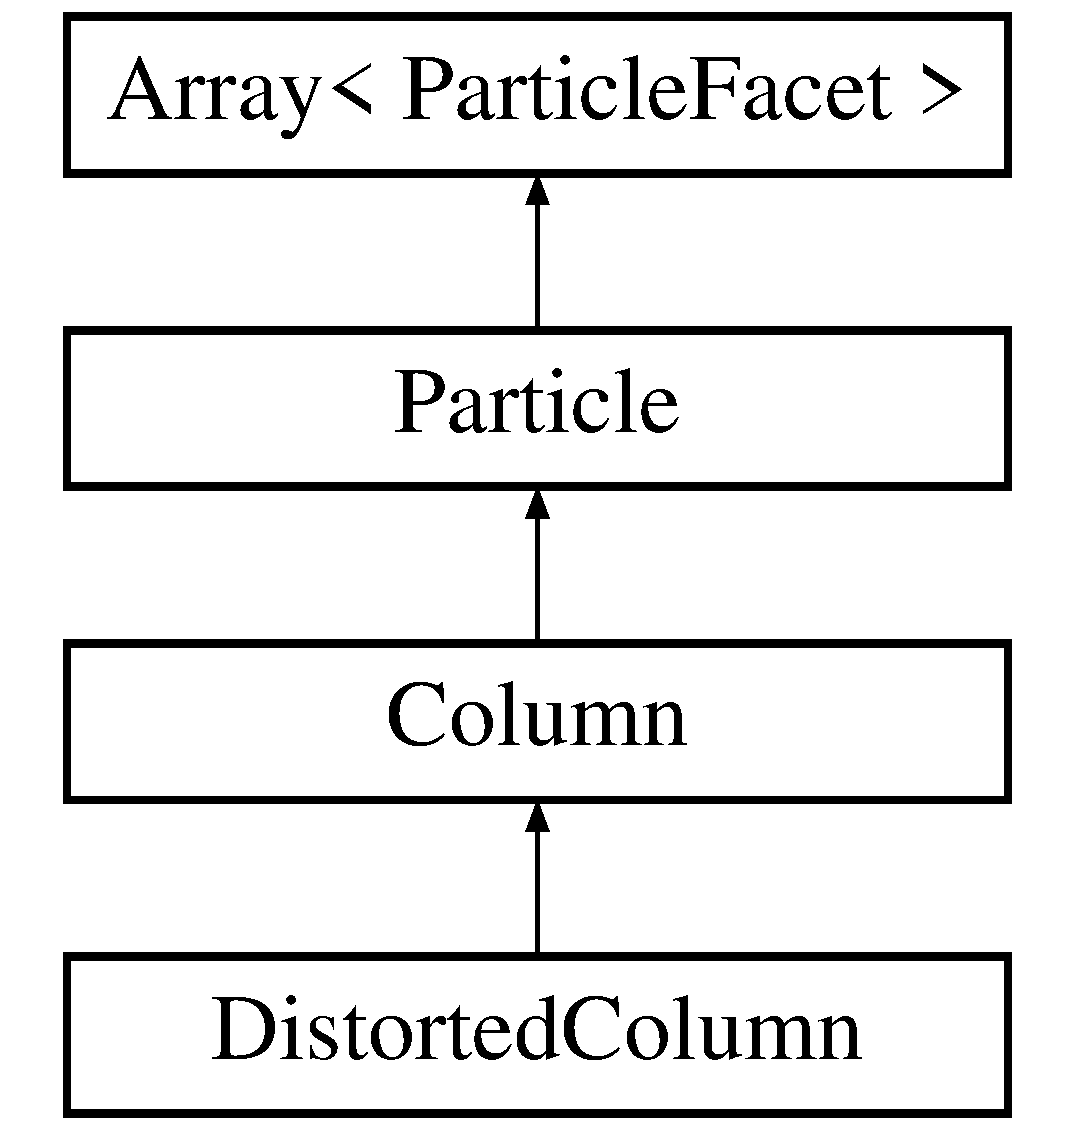
\includegraphics[height=4.000000cm]{class_distorted_column}
\end{center}
\end{figure}
\subsection*{Public Member Functions}
\begin{DoxyCompactItemize}
\item 
\mbox{\Hypertarget{class_distorted_column_a7cc0f6c72403bd2de255297fccbbf92c}\label{class_distorted_column_a7cc0f6c72403bd2de255297fccbbf92c}} 
{\bfseries Distorted\+Column} (const \mbox{\hyperlink{classcomplex}{complex}} \&refr\+Index, const \mbox{\hyperlink{struct_size}{Size}} \&size, double angle)
\end{DoxyCompactItemize}
\subsection*{Additional Inherited Members}


\subsection{Detailed Description}
The Hexagon class The prism particle with 6 number of side facets. 

The documentation for this class was generated from the following files\+:\begin{DoxyCompactItemize}
\item 
particle/Distorted\+Column.\+h\item 
particle/Distorted\+Column.\+cpp\end{DoxyCompactItemize}

\hypertarget{struct_clipper_lib_1_1_double_point}{}\section{Clipper\+Lib\+:\+:Double\+Point Struct Reference}
\label{struct_clipper_lib_1_1_double_point}\index{Clipper\+Lib\+::\+Double\+Point@{Clipper\+Lib\+::\+Double\+Point}}
\subsection*{Public Member Functions}
\begin{DoxyCompactItemize}
\item 
\mbox{\Hypertarget{struct_clipper_lib_1_1_double_point_a3ccbea6aaf488e0a2d8ac499d2676093}\label{struct_clipper_lib_1_1_double_point_a3ccbea6aaf488e0a2d8ac499d2676093}} 
{\bfseries Double\+Point} (double x=0, double y=0)
\item 
\mbox{\Hypertarget{struct_clipper_lib_1_1_double_point_afd33c9193b3cf11536936dc933b965a4}\label{struct_clipper_lib_1_1_double_point_afd33c9193b3cf11536936dc933b965a4}} 
{\bfseries Double\+Point} (\mbox{\hyperlink{struct_clipper_lib_1_1_int_point}{Int\+Point}} ip)
\end{DoxyCompactItemize}
\subsection*{Public Attributes}
\begin{DoxyCompactItemize}
\item 
\mbox{\Hypertarget{struct_clipper_lib_1_1_double_point_a675837cc05f20447313789b82d84ad31}\label{struct_clipper_lib_1_1_double_point_a675837cc05f20447313789b82d84ad31}} 
double {\bfseries X}
\item 
\mbox{\Hypertarget{struct_clipper_lib_1_1_double_point_a49774a93540882d88448badf37034454}\label{struct_clipper_lib_1_1_double_point_a49774a93540882d88448badf37034454}} 
double {\bfseries Y}
\end{DoxyCompactItemize}


The documentation for this struct was generated from the following file\+:\begin{DoxyCompactItemize}
\item 
geometry/clipper/clipper.\+hpp\end{DoxyCompactItemize}

\hypertarget{class_facet}{}\section{Facet Class Reference}
\label{class_facet}\index{Facet@{Facet}}
Inheritance diagram for Facet\+:\begin{figure}[H]
\begin{center}
\leavevmode
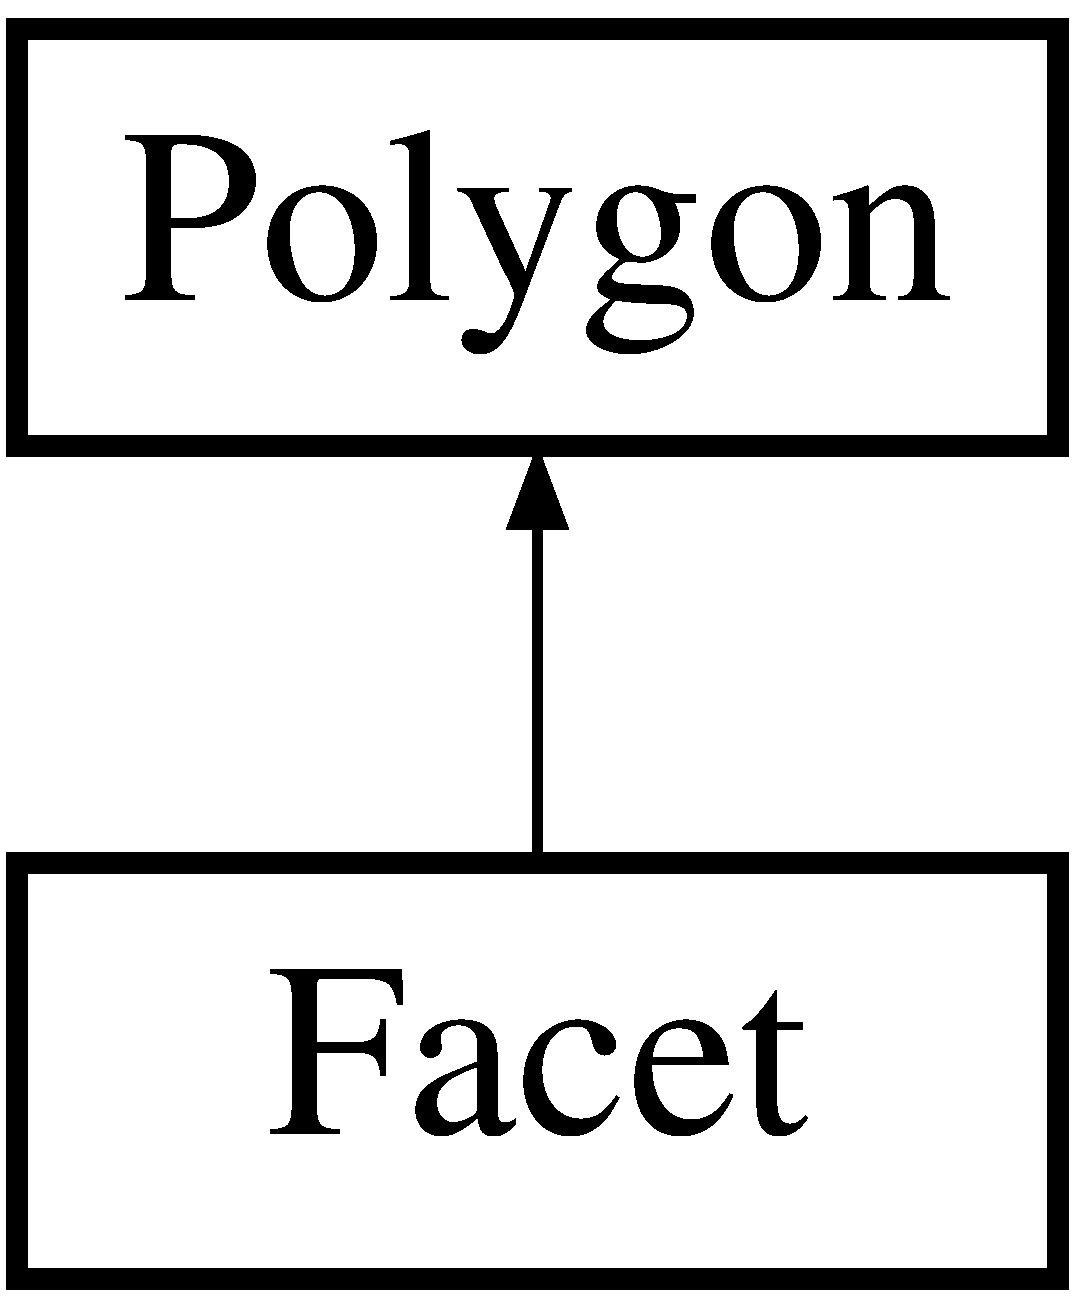
\includegraphics[height=2.000000cm]{class_facet}
\end{center}
\end{figure}
\subsection*{Public Member Functions}
\begin{DoxyCompactItemize}
\item 
\mbox{\Hypertarget{class_facet_a0d3733ac4cb080adb891d61aa53e99a0}\label{class_facet_a0d3733ac4cb080adb891d61aa53e99a0}} 
void {\bfseries Set\+Normal} ()
\item 
\mbox{\Hypertarget{class_facet_a6d79392e22bf04c6569b9a1933f5ca3d}\label{class_facet_a6d79392e22bf04c6569b9a1933f5ca3d}} 
void {\bfseries Set\+Center} ()
\item 
\mbox{\Hypertarget{class_facet_a212a6d0725dcc1102901f4b46153ede2}\label{class_facet_a212a6d0725dcc1102901f4b46153ede2}} 
\mbox{\hyperlink{class_facet}{Facet}} \& {\bfseries operator=} (const \mbox{\hyperlink{class_facet}{Facet}} \&other)
\end{DoxyCompactItemize}
\subsection*{Public Attributes}
\begin{DoxyCompactItemize}
\item 
\mbox{\Hypertarget{class_facet_a082f85a877b24031f8f5d8ffb6ee2a19}\label{class_facet_a082f85a877b24031f8f5d8ffb6ee2a19}} 
int \mbox{\hyperlink{class_facet_a082f85a877b24031f8f5d8ffb6ee2a19}{index}}
\begin{DoxyCompactList}\small\item\em facet index for beam trajectory \end{DoxyCompactList}\item 
\mbox{\Hypertarget{class_facet_a6ce44c6c8de9cd91b4f0d49954871fd0}\label{class_facet_a6ce44c6c8de9cd91b4f0d49954871fd0}} 
\mbox{\hyperlink{struct_point3f}{Point3f}} \mbox{\hyperlink{class_facet_a6ce44c6c8de9cd91b4f0d49954871fd0}{normal}} \mbox{[}2\mbox{]}
\begin{DoxyCompactList}\small\item\em internal and external normals \end{DoxyCompactList}\item 
\mbox{\Hypertarget{class_facet_a6b4c24cba4807b8e4b36663d104d0916}\label{class_facet_a6b4c24cba4807b8e4b36663d104d0916}} 
\mbox{\hyperlink{struct_point3f}{Point3f}} \mbox{\hyperlink{class_facet_a6b4c24cba4807b8e4b36663d104d0916}{center}}
\begin{DoxyCompactList}\small\item\em center of facet polygon (for fast access without calc) \end{DoxyCompactList}\item 
\mbox{\Hypertarget{class_facet_a1a7b54c5a6f7b251acec1fe0cc502baa}\label{class_facet_a1a7b54c5a6f7b251acec1fe0cc502baa}} 
bool {\bfseries is\+Overlayed\+In} = false
\item 
\mbox{\Hypertarget{class_facet_a04433996dfd634bf0c9d5b6a6c196ec9}\label{class_facet_a04433996dfd634bf0c9d5b6a6c196ec9}} 
bool {\bfseries is\+Overlayed\+Out} = false
\end{DoxyCompactItemize}


The documentation for this class was generated from the following files\+:\begin{DoxyCompactItemize}
\item 
geometry/Facet.\+h\item 
geometry/Facet.\+cpp\end{DoxyCompactItemize}

\hypertarget{class_geometry}{}\section{Geometry Class Reference}
\label{class_geometry}\index{Geometry@{Geometry}}
\subsection*{Static Public Member Functions}
\begin{DoxyCompactItemize}
\item 
\mbox{\Hypertarget{class_geometry_a24e8526f076d17a32223293ecb4a2ba8}\label{class_geometry_a24e8526f076d17a32223293ecb4a2ba8}} 
static void {\bfseries Differ\+Polygons} (const \mbox{\hyperlink{class_polygon}{Polygon}} \&subject, const \mbox{\hyperlink{struct_point3f}{Vector3f}} \&subj\+Normal, const \mbox{\hyperlink{class_polygon}{Polygon}} \&clip, const \mbox{\hyperlink{struct_point3f}{Vector3f}} \&clip\+Normal, const \mbox{\hyperlink{struct_point3f}{Vector3f}} \&clip\+Dir, \mbox{\hyperlink{class_polygon_array}{Polygon\+Array}} \&difference)
\item 
\mbox{\Hypertarget{class_geometry_a16820dba38e8321596184a40664f2d3f}\label{class_geometry_a16820dba38e8321596184a40664f2d3f}} 
static \mbox{\hyperlink{struct_point3f}{Point3f}} {\bfseries Project\+Point\+To\+Plane} (const \mbox{\hyperlink{struct_point3f}{Point3f}} \&point, const \mbox{\hyperlink{struct_point3f}{Vector3f}} \&direction, const \mbox{\hyperlink{struct_point3f}{Vector3f}} \&plane\+Normal)
\item 
\mbox{\Hypertarget{class_geometry_a06b703e4b24a60a745c9c9d82f58c3d4}\label{class_geometry_a06b703e4b24a60a745c9c9d82f58c3d4}} 
static bool \mbox{\hyperlink{class_geometry_a06b703e4b24a60a745c9c9d82f58c3d4}{Incident\+Beam\+To\+Facet}} (\mbox{\hyperlink{class_facet}{Facet}} $\ast$facet, const \mbox{\hyperlink{class_polygon}{Polygon}} \&beam\+Pol, bool is\+Inside, const \mbox{\hyperlink{struct_point3f}{Vector3f}} \&inc\+Dir, \mbox{\hyperlink{class_polygon}{Polygon}} \&intersection)
\begin{DoxyCompactList}\small\item\em N\+O\+TE\+: вершины пучка и грани должны быть ориентированы в одном направлении \end{DoxyCompactList}\end{DoxyCompactItemize}


The documentation for this class was generated from the following files\+:\begin{DoxyCompactItemize}
\item 
geometry/geometry\+\_\+lib.\+h\item 
geometry/geometry\+\_\+lib.\+cpp\end{DoxyCompactItemize}

\hypertarget{class_handler}{}\section{Handler Class Reference}
\label{class_handler}\index{Handler@{Handler}}
Inheritance diagram for Handler\+:\begin{figure}[H]
\begin{center}
\leavevmode
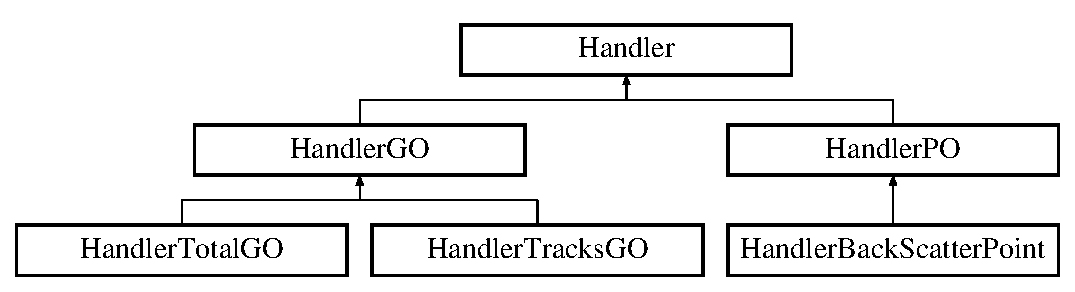
\includegraphics[height=3.000000cm]{class_handler}
\end{center}
\end{figure}
\subsection*{Public Member Functions}
\begin{DoxyCompactItemize}
\item 
\mbox{\Hypertarget{class_handler_a66ed760e6f799ed1c23bb7a6e911877a}\label{class_handler_a66ed760e6f799ed1c23bb7a6e911877a}} 
{\bfseries Handler} (\mbox{\hyperlink{class_particle}{Particle}} $\ast$particle, \mbox{\hyperlink{class_light}{Light}} $\ast$incident\+Light, float wavelength=0)
\item 
\mbox{\Hypertarget{class_handler_a05194b66451cc40133c4bd1a209ad530}\label{class_handler_a05194b66451cc40133c4bd1a209ad530}} 
virtual void {\bfseries Handle\+Beams} (std\+::vector$<$ \mbox{\hyperlink{class_beam}{Beam}} $>$ \&beams)
\item 
\mbox{\Hypertarget{class_handler_a3ef5c3e3392e658c693275a4d46567ba}\label{class_handler_a3ef5c3e3392e658c693275a4d46567ba}} 
virtual void {\bfseries Set\+Tracks} (\mbox{\hyperlink{class_tracks}{Tracks}} $\ast$tracks)
\item 
\mbox{\Hypertarget{class_handler_ae113de0f27a2bac6dbd556c7162aed3e}\label{class_handler_ae113de0f27a2bac6dbd556c7162aed3e}} 
void {\bfseries Set\+Scattering} (\mbox{\hyperlink{class_scattering}{Scattering}} $\ast$scattering)
\item 
\mbox{\Hypertarget{class_handler_a36b5f50775023a5d8acaf5b57e2295b2}\label{class_handler_a36b5f50775023a5d8acaf5b57e2295b2}} 
virtual void {\bfseries Write\+Matrices\+To\+File} (std\+::string \&dest\+Name)
\item 
\mbox{\Hypertarget{class_handler_a4e0616dee14ef67e077209a66f9d48d7}\label{class_handler_a4e0616dee14ef67e077209a66f9d48d7}} 
void {\bfseries Set\+Absorbtion\+Accounting} (bool value)
\item 
\mbox{\Hypertarget{class_handler_af47c4ac1eeb273bd27d8e6688131ff6c}\label{class_handler_af47c4ac1eeb273bd27d8e6688131ff6c}} 
void {\bfseries Set\+Norm\+Index} (double norm\+Index)
\end{DoxyCompactItemize}
\subsection*{Public Attributes}
\begin{DoxyCompactItemize}
\item 
\mbox{\Hypertarget{class_handler_adf74e141c689233565ecc08c7f63b3e8}\label{class_handler_adf74e141c689233565ecc08c7f63b3e8}} 
\mbox{\hyperlink{class_light}{Light}} $\ast$ {\bfseries m\+\_\+incident\+Light}
\end{DoxyCompactItemize}
\subsection*{Protected Member Functions}
\begin{DoxyCompactItemize}
\item 
\mbox{\Hypertarget{class_handler_affc9ffb72eb7ea751f5efa484d7f4ca6}\label{class_handler_affc9ffb72eb7ea751f5efa484d7f4ca6}} 
void {\bfseries Apply\+Absorbtion} (\mbox{\hyperlink{class_beam}{Beam}} \&beam)
\item 
\mbox{\Hypertarget{class_handler_a9216f95781001eb7e73ee16244344e4e}\label{class_handler_a9216f95781001eb7e73ee16244344e4e}} 
double {\bfseries Beam\+Cross\+Section} (const \mbox{\hyperlink{class_beam}{Beam}} \&beam) const
\item 
\mbox{\Hypertarget{class_handler_a1a26cbf9ad33fea2bbd790a188388283}\label{class_handler_a1a26cbf9ad33fea2bbd790a188388283}} 
void {\bfseries Output\+Paths} (const \mbox{\hyperlink{class_beam}{Beam}} \&beam, const \mbox{\hyperlink{struct_optical_path}{Optical\+Path}} \&path)
\end{DoxyCompactItemize}
\subsection*{Protected Attributes}
\begin{DoxyCompactItemize}
\item 
\mbox{\Hypertarget{class_handler_a3ec723e931c7e29d4c170b5952019992}\label{class_handler_a3ec723e931c7e29d4c170b5952019992}} 
\mbox{\hyperlink{class_scattering}{Scattering}} $\ast$ {\bfseries m\+\_\+scattering}
\item 
\mbox{\Hypertarget{class_handler_a6125e2561ea3f9f075c03df319c0c97e}\label{class_handler_a6125e2561ea3f9f075c03df319c0c97e}} 
\mbox{\hyperlink{class_tracks}{Tracks}} $\ast$ {\bfseries m\+\_\+tracks}
\item 
\mbox{\Hypertarget{class_handler_a0df3d2d833e7fda44787d65f81742ebd}\label{class_handler_a0df3d2d833e7fda44787d65f81742ebd}} 
\mbox{\hyperlink{class_particle}{Particle}} $\ast$ {\bfseries m\+\_\+particle}
\item 
\mbox{\Hypertarget{class_handler_af080b55b8049e366b2f2936a72dfda98}\label{class_handler_af080b55b8049e366b2f2936a72dfda98}} 
float {\bfseries m\+\_\+wavelength}
\item 
\mbox{\Hypertarget{class_handler_a9ae74da04772426e9d0cf7769f37feff}\label{class_handler_a9ae74da04772426e9d0cf7769f37feff}} 
bool {\bfseries m\+\_\+has\+Absorbtion}
\item 
\mbox{\Hypertarget{class_handler_a6ea64506e8b2aba07964693d37ab9193}\label{class_handler_a6ea64506e8b2aba07964693d37ab9193}} 
double {\bfseries m\+\_\+norm\+Index}
\item 
\mbox{\Hypertarget{class_handler_a47907a97893becf7a1a57b8aeaf90a9e}\label{class_handler_a47907a97893becf7a1a57b8aeaf90a9e}} 
std\+::ofstream {\bfseries m\+\_\+log\+File}
\item 
\mbox{\Hypertarget{class_handler_a0f06b8309569959b37669991045b8b1d}\label{class_handler_a0f06b8309569959b37669991045b8b1d}} 
std\+::ofstream {\bfseries m\+\_\+abs\+Log\+File}
\item 
\mbox{\Hypertarget{class_handler_ad9af0b7001559831a5abed09014d11d0}\label{class_handler_ad9af0b7001559831a5abed09014d11d0}} 
double {\bfseries m\+\_\+c\+Abs}
\item 
\mbox{\Hypertarget{class_handler_a5de093fc5bccc1d7aa3f60059408c7bc}\label{class_handler_a5de093fc5bccc1d7aa3f60059408c7bc}} 
long long {\bfseries count} = 0
\end{DoxyCompactItemize}


The documentation for this class was generated from the following files\+:\begin{DoxyCompactItemize}
\item 
common/Handler.\+h\item 
common/Handler.\+cpp\end{DoxyCompactItemize}

\hypertarget{class_handler_back_scatter_point}{}\section{Handler\+Back\+Scatter\+Point Class Reference}
\label{class_handler_back_scatter_point}\index{Handler\+Back\+Scatter\+Point@{Handler\+Back\+Scatter\+Point}}


Inheritance diagram for Handler\+Back\+Scatter\+Point\+:
% FIG 0


Collaboration diagram for Handler\+Back\+Scatter\+Point\+:
% FIG 1
\subsection*{Public Member Functions}
\begin{DoxyCompactItemize}
\item 
\mbox{\Hypertarget{class_handler_back_scatter_point_ac1062d361d234fe7f17169cb878000dd}\label{class_handler_back_scatter_point_ac1062d361d234fe7f17169cb878000dd}} 
{\bfseries Handler\+Back\+Scatter\+Point} (\mbox{\hyperlink{class_particle}{Particle}} $\ast$particle, \mbox{\hyperlink{class_light}{Light}} $\ast$incident\+Light, float wavelength=0)
\item 
\mbox{\Hypertarget{class_handler_back_scatter_point_a3ce7fcb7530abbdfd8b1256d7e588536}\label{class_handler_back_scatter_point_a3ce7fcb7530abbdfd8b1256d7e588536}} 
void {\bfseries Handle\+Beams} (std\+::vector$<$ \mbox{\hyperlink{class_beam}{Beam}} $>$ \&beams) override
\item 
\mbox{\Hypertarget{class_handler_back_scatter_point_ac8e90fbda71ee4cde2b4ab92a9929edc}\label{class_handler_back_scatter_point_ac8e90fbda71ee4cde2b4ab92a9929edc}} 
void {\bfseries Set\+Tracks} (\mbox{\hyperlink{class_tracks}{Tracks}} $\ast$tracks) override
\item 
\mbox{\Hypertarget{class_handler_back_scatter_point_a4316e06666856fd593118dcda1879974}\label{class_handler_back_scatter_point_a4316e06666856fd593118dcda1879974}} 
void {\bfseries Output\+Contribution} (\mbox{\hyperlink{class_scattering_files}{Scattering\+Files}} \&files, double angle, double energy, bool is\+Output\+Groups, std\+::string prefix=\char`\"{}\char`\"{})
\end{DoxyCompactItemize}
\subsection*{Additional Inherited Members}


The documentation for this class was generated from the following files\+:\begin{DoxyCompactItemize}
\item 
common/Handler.\+h\item 
common/Handler.\+cpp\end{DoxyCompactItemize}

\hypertarget{class_handler_g_o}{}\section{Handler\+GO Class Reference}
\label{class_handler_g_o}\index{Handler\+GO@{Handler\+GO}}


Inheritance diagram for Handler\+GO\+:
% FIG 0


Collaboration diagram for Handler\+GO\+:
% FIG 1
\subsection*{Public Member Functions}
\begin{DoxyCompactItemize}
\item 
\mbox{\Hypertarget{class_handler_g_o_a45c45f6377f684d741c59f787948ac13}\label{class_handler_g_o_a45c45f6377f684d741c59f787948ac13}} 
{\bfseries Handler\+GO} (\mbox{\hyperlink{class_particle}{Particle}} $\ast$particle, \mbox{\hyperlink{class_light}{Light}} $\ast$incident\+Light, float wavelength=0)
\item 
\mbox{\Hypertarget{class_handler_g_o_a8392befdf6e4cef1d06d7e46b79155f3}\label{class_handler_g_o_a8392befdf6e4cef1d06d7e46b79155f3}} 
void {\bfseries Set\+Tracks} (\mbox{\hyperlink{class_tracks}{Tracks}} $\ast$tracks) override
\item 
\mbox{\Hypertarget{class_handler_g_o_ad5c3f91af1f7c07be11a9a679804cfa0}\label{class_handler_g_o_ad5c3f91af1f7c07be11a9a679804cfa0}} 
double {\bfseries Compute\+Total\+Scattering\+Energy} ()
\item 
\mbox{\Hypertarget{class_handler_g_o_a5b6812ce2b1f202085f12aeb19eaa663}\label{class_handler_g_o_a5b6812ce2b1f202085f12aeb19eaa663}} 
void {\bfseries Write\+Log} (const std\+::string \&str)
\item 
\mbox{\Hypertarget{class_handler_g_o_aec3a04f8bb8188f61acd6a3602a603d1}\label{class_handler_g_o_aec3a04f8bb8188f61acd6a3602a603d1}} 
void {\bfseries Multiply\+Mueller} (const \mbox{\hyperlink{class_beam}{Beam}} \&beam, \mbox{\hyperlink{classmatrix}{matrix}} \&m)
\end{DoxyCompactItemize}
\subsection*{Protected Member Functions}
\begin{DoxyCompactItemize}
\item 
\mbox{\Hypertarget{class_handler_g_o_a5e2e96b14ef9e4152e0b141b68b33cba}\label{class_handler_g_o_a5e2e96b14ef9e4152e0b141b68b33cba}} 
\mbox{\hyperlink{classmatrix}{matrix}} {\bfseries Compute\+Mueller} (int zen\+Ang, \mbox{\hyperlink{class_beam}{Beam}} \&beam)
\item 
\mbox{\Hypertarget{class_handler_g_o_aad730fa5c3975f3fdff91d4e376d3ec8}\label{class_handler_g_o_aad730fa5c3975f3fdff91d4e376d3ec8}} 
void {\bfseries Rotate\+Muller} (const \mbox{\hyperlink{struct_point3f}{Point3f}} \&dir, \mbox{\hyperlink{classmatrix}{matrix}} \&bf)
\item 
\mbox{\Hypertarget{class_handler_g_o_aa0cbf44e161a8c194eae8f9d6e484b25}\label{class_handler_g_o_aa0cbf44e161a8c194eae8f9d6e484b25}} 
void {\bfseries Average\+Over\+Alpha} (int E\+DF, double norm, \mbox{\hyperlink{class_contribution_g_o}{Contribution\+GO}} \&contrib)
\item 
\mbox{\Hypertarget{class_handler_g_o_a287fa480c7124872fc1cd251e7db8c5f}\label{class_handler_g_o_a287fa480c7124872fc1cd251e7db8c5f}} 
void {\bfseries Write\+To\+File} (\mbox{\hyperlink{class_contribution_g_o}{Contribution\+GO}} \&contrib, double norm, const std\+::string \&filename)
\item 
\mbox{\Hypertarget{class_handler_g_o_a4b3c47d02003912688d2aee60c274f21}\label{class_handler_g_o_a4b3c47d02003912688d2aee60c274f21}} 
double {\bfseries Compute\+Optical\+Path\+Absorption} (const \mbox{\hyperlink{class_beam}{Beam}} \&beam)
\item 
\mbox{\Hypertarget{class_handler_g_o_a189f1f533f10a64afa5b9aac207d85fe}\label{class_handler_g_o_a189f1f533f10a64afa5b9aac207d85fe}} 
\mbox{\hyperlink{struct_point3f}{Point3f}} {\bfseries CalcK} (std\+::vector$<$ int $>$ \&tr)
\end{DoxyCompactItemize}
\subsection*{Protected Attributes}
\begin{DoxyCompactItemize}
\item 
\mbox{\Hypertarget{class_handler_g_o_afa1081e6a7cbdde1f843c90ddac65778}\label{class_handler_g_o_afa1081e6a7cbdde1f843c90ddac65778}} 
\mbox{\hyperlink{class_contribution_g_o}{Contribution\+GO}} {\bfseries m\+\_\+total\+Contrib}
\item 
\mbox{\Hypertarget{class_handler_g_o_ad381fe7c0a1c4031e46b8660a2cfe630}\label{class_handler_g_o_ad381fe7c0a1c4031e46b8660a2cfe630}} 
std\+::vector$<$ \mbox{\hyperlink{class_contribution_g_o}{Contribution\+GO}} $>$ {\bfseries m\+\_\+tracks\+Contrib}
\item 
\mbox{\Hypertarget{class_handler_g_o_a6c7a6e0a06070cc89495d0276092ed2f}\label{class_handler_g_o_a6c7a6e0a06070cc89495d0276092ed2f}} 
double {\bfseries m\+\_\+sin\+Angle}
\end{DoxyCompactItemize}
\subsection*{Additional Inherited Members}


The documentation for this class was generated from the following files\+:\begin{DoxyCompactItemize}
\item 
common/Handler.\+h\item 
common/Handler.\+cpp\end{DoxyCompactItemize}

\hypertarget{class_handler_p_o}{}\section{Handler\+PO Class Reference}
\label{class_handler_p_o}\index{Handler\+PO@{Handler\+PO}}
Inheritance diagram for Handler\+PO\+:\begin{figure}[H]
\begin{center}
\leavevmode
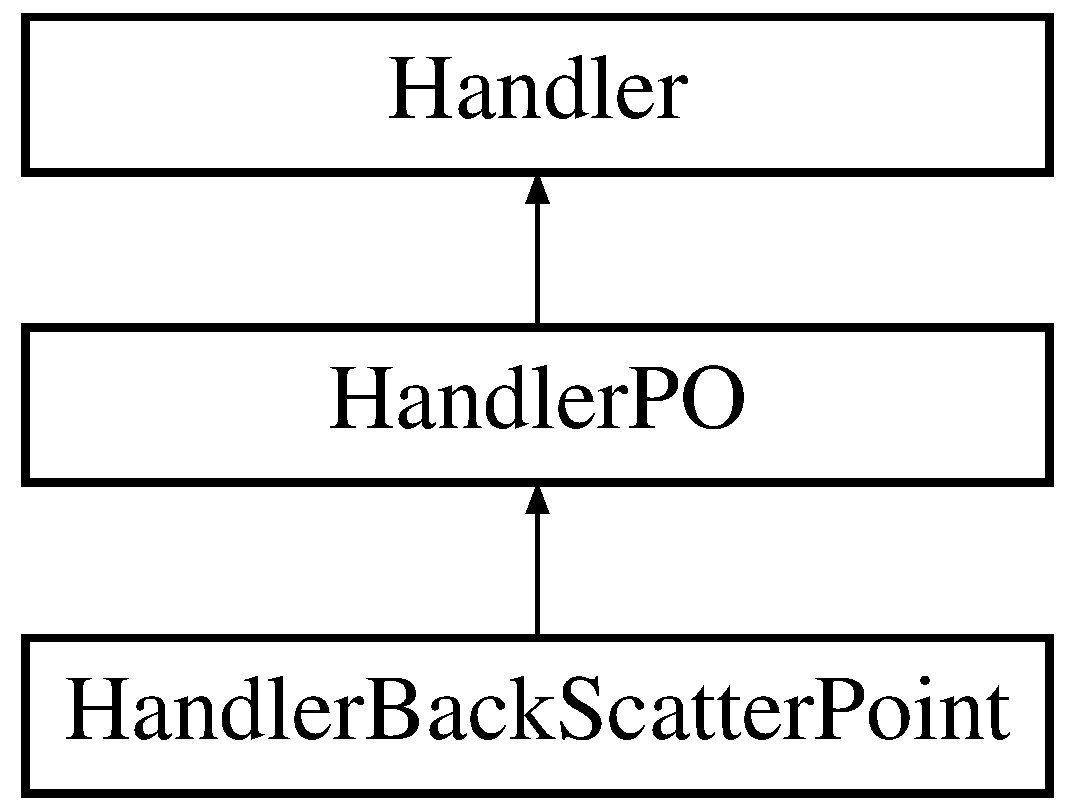
\includegraphics[height=3.000000cm]{class_handler_p_o}
\end{center}
\end{figure}
\subsection*{Public Member Functions}
\begin{DoxyCompactItemize}
\item 
\mbox{\Hypertarget{class_handler_p_o_ae4e146c9650b371deaeb6aa487e67928}\label{class_handler_p_o_ae4e146c9650b371deaeb6aa487e67928}} 
{\bfseries Handler\+PO} (\mbox{\hyperlink{class_particle}{Particle}} $\ast$particle, \mbox{\hyperlink{class_light}{Light}} $\ast$incident\+Light, float wavelength=0)
\item 
\mbox{\Hypertarget{class_handler_p_o_a34614f0dab5f801ad4588fa5d1e0825d}\label{class_handler_p_o_a34614f0dab5f801ad4588fa5d1e0825d}} 
void {\bfseries Handle\+Beams} (std\+::vector$<$ \mbox{\hyperlink{class_beam}{Beam}} $>$ \&beams) override
\item 
\mbox{\Hypertarget{class_handler_p_o_acd1699ce858357c838f4a2507013b4aa}\label{class_handler_p_o_acd1699ce858357c838f4a2507013b4aa}} 
void {\bfseries Write\+Matrices\+To\+File} (std\+::string \&dest\+Name) override
\item 
\mbox{\Hypertarget{class_handler_p_o_a0a25182f4636d39a85f00ff1c78dd833}\label{class_handler_p_o_a0a25182f4636d39a85f00ff1c78dd833}} 
void {\bfseries Set\+Scattering\+Conus} (const \mbox{\hyperlink{struct_conus}{Conus}} \&conus)
\item 
\mbox{\Hypertarget{class_handler_p_o_a5587518a68abb18ad556ec4f3521e397}\label{class_handler_p_o_a5587518a68abb18ad556ec4f3521e397}} 
void {\bfseries set\+Con20} (bool value)
\end{DoxyCompactItemize}
\subsection*{Protected Member Functions}
\begin{DoxyCompactItemize}
\item 
\mbox{\Hypertarget{class_handler_p_o_a65a3e8c8a580a321b315f8afe89dd34e}\label{class_handler_p_o_a65a3e8c8a580a321b315f8afe89dd34e}} 
void {\bfseries Apply\+Diffraction} (const \mbox{\hyperlink{class_beam}{Beam}} \&beam, const \mbox{\hyperlink{struct_point3f}{Point3f}} \&beam\+Basis, const \mbox{\hyperlink{struct_point3d}{Vector3d}} \&vf, const \mbox{\hyperlink{struct_point3d}{Vector3d}} \&vr, const \mbox{\hyperlink{classmatrix_c}{matrixC}} \&fn\+Jones, \mbox{\hyperlink{classmatrix_c}{matrixC}} \&jones)
\item 
\mbox{\Hypertarget{class_handler_p_o_a50d3c2cdc831fffb663487f75d47513a}\label{class_handler_p_o_a50d3c2cdc831fffb663487f75d47513a}} 
void {\bfseries Rotate\+Jones} (const \mbox{\hyperlink{class_beam}{Beam}} \&beam, const \mbox{\hyperlink{struct_point3f}{Vector3f}} \&T, const \mbox{\hyperlink{struct_point3d}{Vector3d}} \&vf, const \mbox{\hyperlink{struct_point3d}{Vector3d}} \&vr, \mbox{\hyperlink{classmatrix_c}{matrixC}} \&J)
\item 
\mbox{\Hypertarget{class_handler_p_o_a82d6ec400230d75e175f1f4ab300e323}\label{class_handler_p_o_a82d6ec400230d75e175f1f4ab300e323}} 
void {\bfseries CleanJ} ()
\item 
\mbox{\Hypertarget{class_handler_p_o_a01b025f232ece30a670b53f4acdf4e78}\label{class_handler_p_o_a01b025f232ece30a670b53f4acdf4e78}} 
void {\bfseries Add\+To\+Mueller} ()
\item 
\mbox{\Hypertarget{class_handler_p_o_a38248eea6a5b4a2cd53f4cfc57c66a4d}\label{class_handler_p_o_a38248eea6a5b4a2cd53f4cfc57c66a4d}} 
\mbox{\hyperlink{classmatrix_c}{matrixC}} {\bfseries Compute\+Fn\+Jones} (const \mbox{\hyperlink{class_matrix2x2c}{Matrix2x2c}} \&jones, const \mbox{\hyperlink{struct_point3d}{Point3d}} \&center, const \mbox{\hyperlink{struct_point3d}{Vector3d}} \&vr, double proj\+Lenght)
\end{DoxyCompactItemize}
\subsection*{Protected Attributes}
\begin{DoxyCompactItemize}
\item 
\mbox{\Hypertarget{class_handler_p_o_a7feb7cb39223e0eda119c7f4b6aa2ace}\label{class_handler_p_o_a7feb7cb39223e0eda119c7f4b6aa2ace}} 
std\+::vector$<$ \mbox{\hyperlink{class_arr2_d_c}{Arr2\+DC}} $>$ {\bfseries J}
\item 
\mbox{\Hypertarget{class_handler_p_o_a158f16b20185bb8790e602e51a32e81d}\label{class_handler_p_o_a158f16b20185bb8790e602e51a32e81d}} 
\mbox{\hyperlink{class_arr2_d}{Arr2D}} {\bfseries M}
\item 
\mbox{\Hypertarget{class_handler_p_o_a8a23d47a3971ab91786b3ea9b861d38d}\label{class_handler_p_o_a8a23d47a3971ab91786b3ea9b861d38d}} 
\mbox{\hyperlink{struct_conus}{Conus}} {\bfseries m\+\_\+conus}
\item 
\mbox{\Hypertarget{class_handler_p_o_a4719cc4f40a41adea1c1e05c60eba146}\label{class_handler_p_o_a4719cc4f40a41adea1c1e05c60eba146}} 
bool {\bfseries is\+Nan\+Occured} = false
\item 
\mbox{\Hypertarget{class_handler_p_o_a054af595516ef6050a06aa87899073e3}\label{class_handler_p_o_a054af595516ef6050a06aa87899073e3}} 
bool {\bfseries is\+Nan} = false
\item 
\mbox{\Hypertarget{class_handler_p_o_af10369da142ec20f430d2db0997994e4}\label{class_handler_p_o_af10369da142ec20f430d2db0997994e4}} 
bool {\bfseries con20} = true
\end{DoxyCompactItemize}
\subsection*{Additional Inherited Members}


The documentation for this class was generated from the following files\+:\begin{DoxyCompactItemize}
\item 
common/Handler.\+h\item 
common/Handler.\+cpp\end{DoxyCompactItemize}

\hypertarget{class_handler_total_g_o}{}\section{Handler\+Total\+GO Class Reference}
\label{class_handler_total_g_o}\index{Handler\+Total\+GO@{Handler\+Total\+GO}}


Inheritance diagram for Handler\+Total\+GO\+:
% FIG 0


Collaboration diagram for Handler\+Total\+GO\+:
% FIG 1
\subsection*{Public Member Functions}
\begin{DoxyCompactItemize}
\item 
\mbox{\Hypertarget{class_handler_total_g_o_a875f12f02fcb152d084b249a353f523e}\label{class_handler_total_g_o_a875f12f02fcb152d084b249a353f523e}} 
{\bfseries Handler\+Total\+GO} (\mbox{\hyperlink{class_particle}{Particle}} $\ast$particle, \mbox{\hyperlink{class_light}{Light}} $\ast$incident\+Light, float wavelength=0)
\item 
\mbox{\Hypertarget{class_handler_total_g_o_ad8500e02d66519a915ad9156114df614}\label{class_handler_total_g_o_ad8500e02d66519a915ad9156114df614}} 
void {\bfseries Handle\+Beams} (std\+::vector$<$ \mbox{\hyperlink{class_beam}{Beam}} $>$ \&beams) override
\item 
\mbox{\Hypertarget{class_handler_total_g_o_a3548dbfd472665c922958af65ff576ec}\label{class_handler_total_g_o_a3548dbfd472665c922958af65ff576ec}} 
void {\bfseries Write\+Matrices\+To\+File} (std\+::string \&dest\+Name) override
\end{DoxyCompactItemize}
\subsection*{Additional Inherited Members}


The documentation for this class was generated from the following files\+:\begin{DoxyCompactItemize}
\item 
common/Handler.\+h\item 
common/Handler.\+cpp\end{DoxyCompactItemize}

\hypertarget{class_handler_tracks_g_o}{}\section{Handler\+Tracks\+GO Class Reference}
\label{class_handler_tracks_g_o}\index{Handler\+Tracks\+GO@{Handler\+Tracks\+GO}}


Inheritance diagram for Handler\+Tracks\+GO\+:
% FIG 0


Collaboration diagram for Handler\+Tracks\+GO\+:
% FIG 1
\subsection*{Public Member Functions}
\begin{DoxyCompactItemize}
\item 
\mbox{\Hypertarget{class_handler_tracks_g_o_a991b2082b340c3951e8a07dcca7faac7}\label{class_handler_tracks_g_o_a991b2082b340c3951e8a07dcca7faac7}} 
{\bfseries Handler\+Tracks\+GO} (\mbox{\hyperlink{class_particle}{Particle}} $\ast$particle, \mbox{\hyperlink{class_light}{Light}} $\ast$incident\+Light, float wavelength=0)
\item 
\mbox{\Hypertarget{class_handler_tracks_g_o_a0968818f112c86548db0f841667dde4f}\label{class_handler_tracks_g_o_a0968818f112c86548db0f841667dde4f}} 
void {\bfseries Handle\+Beams} (std\+::vector$<$ \mbox{\hyperlink{class_beam}{Beam}} $>$ \&beams) override
\item 
\mbox{\Hypertarget{class_handler_tracks_g_o_a7a14a10b0d8b54039cf2c9000b0f1d51}\label{class_handler_tracks_g_o_a7a14a10b0d8b54039cf2c9000b0f1d51}} 
void {\bfseries Write\+Matrices\+To\+File} (std\+::string \&dest\+Name) override
\end{DoxyCompactItemize}
\subsection*{Additional Inherited Members}


The documentation for this class was generated from the following files\+:\begin{DoxyCompactItemize}
\item 
common/Handler.\+h\item 
common/Handler.\+cpp\end{DoxyCompactItemize}

\hypertarget{class_hexagonal_aggregate}{}\section{Hexagonal\+Aggregate Class Reference}
\label{class_hexagonal_aggregate}\index{Hexagonal\+Aggregate@{Hexagonal\+Aggregate}}


Inheritance diagram for Hexagonal\+Aggregate\+:
% FIG 0


Collaboration diagram for Hexagonal\+Aggregate\+:
% FIG 1
\subsection*{Public Member Functions}
\begin{DoxyCompactItemize}
\item 
\mbox{\Hypertarget{class_hexagonal_aggregate_a3ebac4728ad288d82ac7506c1e4a6d16}\label{class_hexagonal_aggregate_a3ebac4728ad288d82ac7506c1e4a6d16}} 
{\bfseries Hexagonal\+Aggregate} (const \mbox{\hyperlink{classcomplex}{complex}} \&refr\+Index, const \mbox{\hyperlink{struct_size}{Size}} \&size, int particle\+Number)
\end{DoxyCompactItemize}
\subsection*{Protected Member Functions}
\begin{DoxyCompactItemize}
\item 
\mbox{\Hypertarget{class_hexagonal_aggregate_af6bec3e2933468de2d82efb7368bb7d1}\label{class_hexagonal_aggregate_af6bec3e2933468de2d82efb7368bb7d1}} 
void {\bfseries Set\+Facet\+Params} () override
\end{DoxyCompactItemize}
\subsection*{Additional Inherited Members}


The documentation for this class was generated from the following files\+:\begin{DoxyCompactItemize}
\item 
particle/Hexagonal\+Aggregate.\+h\item 
particle/Hexagonal\+Aggregate.\+cpp\end{DoxyCompactItemize}

\hypertarget{class_hollow_column}{}\section{Hollow\+Column Class Reference}
\label{class_hollow_column}\index{Hollow\+Column@{Hollow\+Column}}


The Concave\+Hexagonal class The prism particle with 6 number of side facets and 2 cavities on the base facets.  




{\ttfamily \#include $<$Hollow\+Column.\+h$>$}

Inheritance diagram for Hollow\+Column\+:\begin{figure}[H]
\begin{center}
\leavevmode
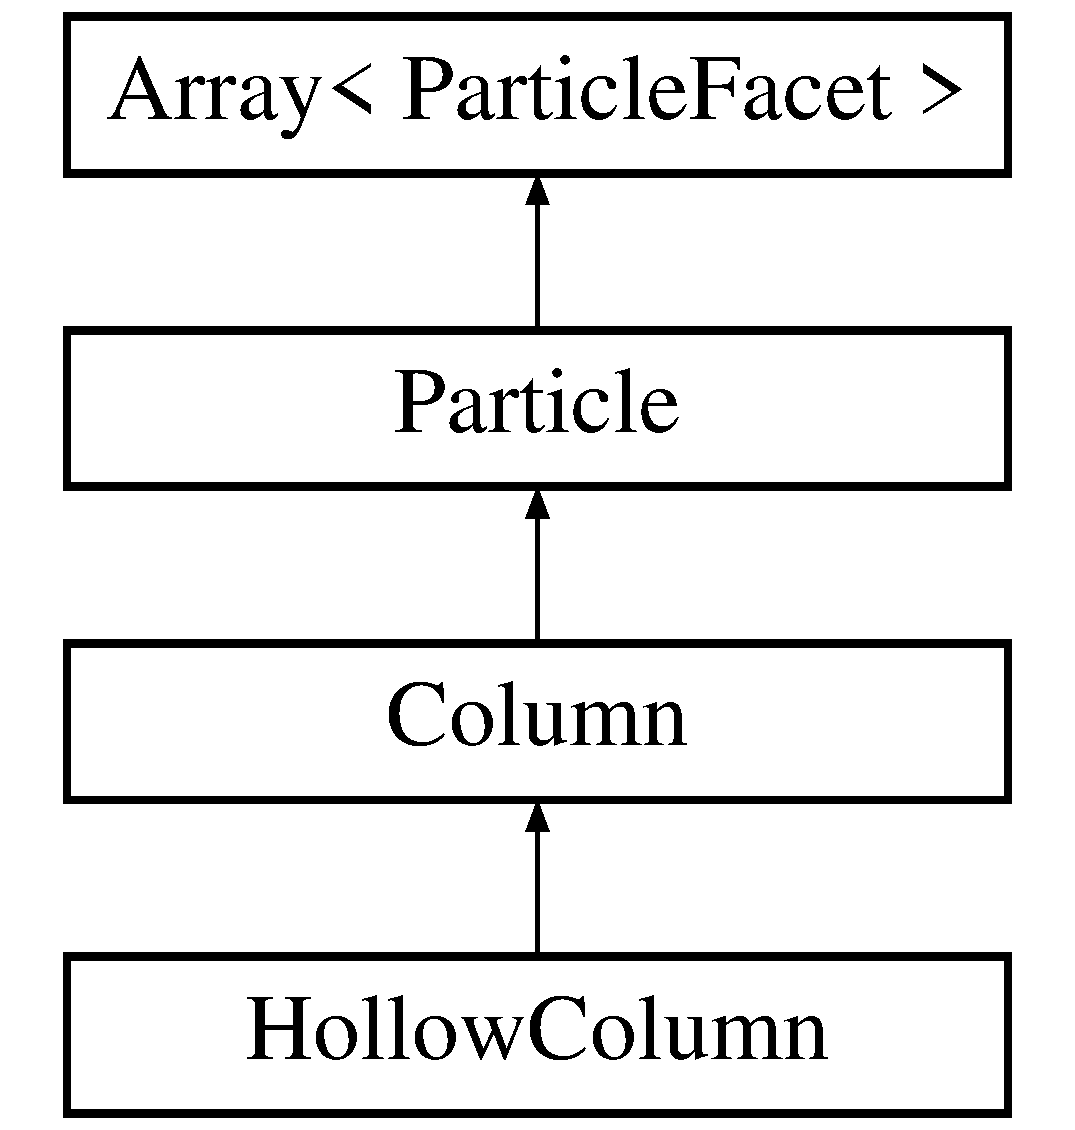
\includegraphics[height=4.000000cm]{class_hollow_column}
\end{center}
\end{figure}
\subsection*{Public Member Functions}
\begin{DoxyCompactItemize}
\item 
\mbox{\Hypertarget{class_hollow_column_ac03a1b9311904c85ffe890ec794401c1}\label{class_hollow_column_ac03a1b9311904c85ffe890ec794401c1}} 
{\bfseries Hollow\+Column} (const \mbox{\hyperlink{classcomplex}{complex}} \&refr\+Index, const \mbox{\hyperlink{struct_size}{Size}} \&size, double cavity\+Angle)
\end{DoxyCompactItemize}
\subsection*{Protected Member Functions}
\begin{DoxyCompactItemize}
\item 
\mbox{\Hypertarget{class_hollow_column_a91310788744ca94657fd8d483f955ccf}\label{class_hollow_column_a91310788744ca94657fd8d483f955ccf}} 
void {\bfseries Set\+Facet\+Params} () override
\end{DoxyCompactItemize}
\subsection*{Additional Inherited Members}


\subsection{Detailed Description}
The Concave\+Hexagonal class The prism particle with 6 number of side facets and 2 cavities on the base facets. 

The documentation for this class was generated from the following files\+:\begin{DoxyCompactItemize}
\item 
particle/Hollow\+Column.\+h\item 
particle/Hollow\+Column.\+cpp\end{DoxyCompactItemize}

\hypertarget{class_incidence}{}\section{Incidence Class Reference}
\label{class_incidence}\index{Incidence@{Incidence}}


Inheritance diagram for Incidence\+:
% FIG 0
\subsection*{Public Member Functions}
\begin{DoxyCompactItemize}
\item 
\mbox{\Hypertarget{class_incidence_af17d5c74ea2928c821c799cf026aa35c}\label{class_incidence_af17d5c74ea2928c821c799cf026aa35c}} 
virtual void {\bfseries Compute\+Directions} (\mbox{\hyperlink{class_beam}{Beam}} \&, \mbox{\hyperlink{class_splitting}{Splitting}} \&) const
\item 
\mbox{\Hypertarget{class_incidence_a205492fd20d495d89948b4a0bebd7da3}\label{class_incidence_a205492fd20d495d89948b4a0bebd7da3}} 
virtual void {\bfseries Compute\+Jones\+Matrices} (\mbox{\hyperlink{class_beam}{Beam}} \&, \mbox{\hyperlink{class_splitting}{Splitting}} \&) const
\item 
\mbox{\Hypertarget{class_incidence_aeb94474ae1bf08abaf3c18e0500b96bd}\label{class_incidence_aeb94474ae1bf08abaf3c18e0500b96bd}} 
void {\bfseries Compute\+Optical\+Paths} (const \mbox{\hyperlink{class_beam}{Beam}} \&beam, \mbox{\hyperlink{class_splitting}{Splitting}} \&splitter) const
\end{DoxyCompactItemize}


The documentation for this class was generated from the following files\+:\begin{DoxyCompactItemize}
\item 
incidence/Incidence.\+h\item 
incidence/Incidence.\+cpp\end{DoxyCompactItemize}

\hypertarget{class_clipper_lib_1_1_int128}{}\section{Clipper\+Lib\+:\+:Int128 Class Reference}
\label{class_clipper_lib_1_1_int128}\index{Clipper\+Lib\+::\+Int128@{Clipper\+Lib\+::\+Int128}}
\subsection*{Public Member Functions}
\begin{DoxyCompactItemize}
\item 
\mbox{\Hypertarget{class_clipper_lib_1_1_int128_acb7953a56e0ddb6d3245268e457f9e37}\label{class_clipper_lib_1_1_int128_acb7953a56e0ddb6d3245268e457f9e37}} 
{\bfseries Int128} (long64 \+\_\+lo=0)
\item 
\mbox{\Hypertarget{class_clipper_lib_1_1_int128_ad113c3dc3bd371984b05fddb1fe527e2}\label{class_clipper_lib_1_1_int128_ad113c3dc3bd371984b05fddb1fe527e2}} 
{\bfseries Int128} (const \mbox{\hyperlink{class_clipper_lib_1_1_int128}{Int128}} \&val)
\item 
\mbox{\Hypertarget{class_clipper_lib_1_1_int128_ac23a17a6a5ea143f0297b7ba0dd1830e}\label{class_clipper_lib_1_1_int128_ac23a17a6a5ea143f0297b7ba0dd1830e}} 
{\bfseries Int128} (const long64 \&\+\_\+hi, const ulong64 \&\+\_\+lo)
\item 
\mbox{\Hypertarget{class_clipper_lib_1_1_int128_a908b1ffab7e190f8db9d2adccbb9eef4}\label{class_clipper_lib_1_1_int128_a908b1ffab7e190f8db9d2adccbb9eef4}} 
\mbox{\hyperlink{class_clipper_lib_1_1_int128}{Int128}} \& {\bfseries operator=} (const long64 \&val)
\item 
\mbox{\Hypertarget{class_clipper_lib_1_1_int128_a8946a96471d06371fd5ea4f4f65cb4c9}\label{class_clipper_lib_1_1_int128_a8946a96471d06371fd5ea4f4f65cb4c9}} 
bool {\bfseries operator==} (const \mbox{\hyperlink{class_clipper_lib_1_1_int128}{Int128}} \&val) const
\item 
\mbox{\Hypertarget{class_clipper_lib_1_1_int128_ae7437e8f6dcb611e8b33e5e7c9c8fbc0}\label{class_clipper_lib_1_1_int128_ae7437e8f6dcb611e8b33e5e7c9c8fbc0}} 
bool {\bfseries operator!=} (const \mbox{\hyperlink{class_clipper_lib_1_1_int128}{Int128}} \&val) const
\item 
\mbox{\Hypertarget{class_clipper_lib_1_1_int128_ac3d844564066e223483f9393ba050daa}\label{class_clipper_lib_1_1_int128_ac3d844564066e223483f9393ba050daa}} 
bool {\bfseries operator$>$} (const \mbox{\hyperlink{class_clipper_lib_1_1_int128}{Int128}} \&val) const
\item 
\mbox{\Hypertarget{class_clipper_lib_1_1_int128_ab55bb6a363e7ced8e5e64a1eefac6000}\label{class_clipper_lib_1_1_int128_ab55bb6a363e7ced8e5e64a1eefac6000}} 
bool {\bfseries operator$<$} (const \mbox{\hyperlink{class_clipper_lib_1_1_int128}{Int128}} \&val) const
\item 
\mbox{\Hypertarget{class_clipper_lib_1_1_int128_af01cfcc3d7bdeffc25e2efb855cd196e}\label{class_clipper_lib_1_1_int128_af01cfcc3d7bdeffc25e2efb855cd196e}} 
bool {\bfseries operator$>$=} (const \mbox{\hyperlink{class_clipper_lib_1_1_int128}{Int128}} \&val) const
\item 
\mbox{\Hypertarget{class_clipper_lib_1_1_int128_ab3667a2abe7b05841b8004496e4e5ddd}\label{class_clipper_lib_1_1_int128_ab3667a2abe7b05841b8004496e4e5ddd}} 
bool {\bfseries operator$<$=} (const \mbox{\hyperlink{class_clipper_lib_1_1_int128}{Int128}} \&val) const
\item 
\mbox{\Hypertarget{class_clipper_lib_1_1_int128_ad48a700134ab5c4e08bd53966b731950}\label{class_clipper_lib_1_1_int128_ad48a700134ab5c4e08bd53966b731950}} 
\mbox{\hyperlink{class_clipper_lib_1_1_int128}{Int128}} \& {\bfseries operator+=} (const \mbox{\hyperlink{class_clipper_lib_1_1_int128}{Int128}} \&rhs)
\item 
\mbox{\Hypertarget{class_clipper_lib_1_1_int128_ad32b1394a82ddf0d9f7da299b91212bd}\label{class_clipper_lib_1_1_int128_ad32b1394a82ddf0d9f7da299b91212bd}} 
\mbox{\hyperlink{class_clipper_lib_1_1_int128}{Int128}} {\bfseries operator+} (const \mbox{\hyperlink{class_clipper_lib_1_1_int128}{Int128}} \&rhs) const
\item 
\mbox{\Hypertarget{class_clipper_lib_1_1_int128_a7b35c74c15392ae8d48c031f750c1b28}\label{class_clipper_lib_1_1_int128_a7b35c74c15392ae8d48c031f750c1b28}} 
\mbox{\hyperlink{class_clipper_lib_1_1_int128}{Int128}} \& {\bfseries operator-\/=} (const \mbox{\hyperlink{class_clipper_lib_1_1_int128}{Int128}} \&rhs)
\item 
\mbox{\Hypertarget{class_clipper_lib_1_1_int128_a8e8d49476d9cecd1f585790f55dcd8da}\label{class_clipper_lib_1_1_int128_a8e8d49476d9cecd1f585790f55dcd8da}} 
\mbox{\hyperlink{class_clipper_lib_1_1_int128}{Int128}} {\bfseries operator-\/} (const \mbox{\hyperlink{class_clipper_lib_1_1_int128}{Int128}} \&rhs) const
\item 
\mbox{\Hypertarget{class_clipper_lib_1_1_int128_a10758b3c62928c3ed45298465b43992c}\label{class_clipper_lib_1_1_int128_a10758b3c62928c3ed45298465b43992c}} 
\mbox{\hyperlink{class_clipper_lib_1_1_int128}{Int128}} {\bfseries operator-\/} () const
\item 
\mbox{\Hypertarget{class_clipper_lib_1_1_int128_aff43efe690619303c4b0a513834d5296}\label{class_clipper_lib_1_1_int128_aff43efe690619303c4b0a513834d5296}} 
{\bfseries operator double} () const
\end{DoxyCompactItemize}
\subsection*{Public Attributes}
\begin{DoxyCompactItemize}
\item 
\mbox{\Hypertarget{class_clipper_lib_1_1_int128_a991b9da6e53c777a94fca640e505b258}\label{class_clipper_lib_1_1_int128_a991b9da6e53c777a94fca640e505b258}} 
ulong64 {\bfseries lo}
\item 
\mbox{\Hypertarget{class_clipper_lib_1_1_int128_a167643d0860a14fb563e055511e15e14}\label{class_clipper_lib_1_1_int128_a167643d0860a14fb563e055511e15e14}} 
long64 {\bfseries hi}
\end{DoxyCompactItemize}


The documentation for this class was generated from the following file\+:\begin{DoxyCompactItemize}
\item 
geometry/clipper/clipper.\+cpp\end{DoxyCompactItemize}

\hypertarget{struct_clipper_lib_1_1_intersect_node}{}\section{Clipper\+Lib\+:\+:Intersect\+Node Struct Reference}
\label{struct_clipper_lib_1_1_intersect_node}\index{Clipper\+Lib\+::\+Intersect\+Node@{Clipper\+Lib\+::\+Intersect\+Node}}
\subsection*{Public Attributes}
\begin{DoxyCompactItemize}
\item 
\mbox{\Hypertarget{struct_clipper_lib_1_1_intersect_node_a43fd790cc38441edb594841d79b25f13}\label{struct_clipper_lib_1_1_intersect_node_a43fd790cc38441edb594841d79b25f13}} 
\mbox{\hyperlink{struct_clipper_lib_1_1_t_edge}{T\+Edge}} $\ast$ {\bfseries Edge1}
\item 
\mbox{\Hypertarget{struct_clipper_lib_1_1_intersect_node_afcb56e7564fedf1c90962a9f75454539}\label{struct_clipper_lib_1_1_intersect_node_afcb56e7564fedf1c90962a9f75454539}} 
\mbox{\hyperlink{struct_clipper_lib_1_1_t_edge}{T\+Edge}} $\ast$ {\bfseries Edge2}
\item 
\mbox{\Hypertarget{struct_clipper_lib_1_1_intersect_node_a91fc92370fb47797dae0602443e6475e}\label{struct_clipper_lib_1_1_intersect_node_a91fc92370fb47797dae0602443e6475e}} 
\mbox{\hyperlink{struct_clipper_lib_1_1_int_point}{Int\+Point}} {\bfseries Pt}
\end{DoxyCompactItemize}


The documentation for this struct was generated from the following file\+:\begin{DoxyCompactItemize}
\item 
geometry/clipper/clipper.\+cpp\end{DoxyCompactItemize}

\hypertarget{struct_clipper_lib_1_1_int_point}{}\section{Clipper\+Lib\+:\+:Int\+Point Struct Reference}
\label{struct_clipper_lib_1_1_int_point}\index{Clipper\+Lib\+::\+Int\+Point@{Clipper\+Lib\+::\+Int\+Point}}
\subsection*{Public Member Functions}
\begin{DoxyCompactItemize}
\item 
\mbox{\Hypertarget{struct_clipper_lib_1_1_int_point_aa43aba31684a398962bee5a56d6d378a}\label{struct_clipper_lib_1_1_int_point_aa43aba31684a398962bee5a56d6d378a}} 
{\bfseries Int\+Point} (c\+Int x=0, c\+Int y=0, c\+Int z=0)
\end{DoxyCompactItemize}
\subsection*{Public Attributes}
\begin{DoxyCompactItemize}
\item 
\mbox{\Hypertarget{struct_clipper_lib_1_1_int_point_a608d16d39c8762e6c3c0a688efb310b6}\label{struct_clipper_lib_1_1_int_point_a608d16d39c8762e6c3c0a688efb310b6}} 
c\+Int {\bfseries X}
\item 
\mbox{\Hypertarget{struct_clipper_lib_1_1_int_point_a8445d190cd9013bb34d49b5a8a240425}\label{struct_clipper_lib_1_1_int_point_a8445d190cd9013bb34d49b5a8a240425}} 
c\+Int {\bfseries Y}
\item 
\mbox{\Hypertarget{struct_clipper_lib_1_1_int_point_a9194e50a264eefb93cfcf5a16f882e9e}\label{struct_clipper_lib_1_1_int_point_a9194e50a264eefb93cfcf5a16f882e9e}} 
c\+Int {\bfseries Z}
\end{DoxyCompactItemize}
\subsection*{Friends}
\begin{DoxyCompactItemize}
\item 
\mbox{\Hypertarget{struct_clipper_lib_1_1_int_point_a6afef09ee09723a387e3046287e2635b}\label{struct_clipper_lib_1_1_int_point_a6afef09ee09723a387e3046287e2635b}} 
bool {\bfseries operator==} (const \mbox{\hyperlink{struct_clipper_lib_1_1_int_point}{Int\+Point}} \&a, const \mbox{\hyperlink{struct_clipper_lib_1_1_int_point}{Int\+Point}} \&b)
\item 
\mbox{\Hypertarget{struct_clipper_lib_1_1_int_point_aa37b2afb6cbc44cb9cd13ecc009decfb}\label{struct_clipper_lib_1_1_int_point_aa37b2afb6cbc44cb9cd13ecc009decfb}} 
bool {\bfseries operator!=} (const \mbox{\hyperlink{struct_clipper_lib_1_1_int_point}{Int\+Point}} \&a, const \mbox{\hyperlink{struct_clipper_lib_1_1_int_point}{Int\+Point}} \&b)
\end{DoxyCompactItemize}


The documentation for this struct was generated from the following file\+:\begin{DoxyCompactItemize}
\item 
geometry/clipper/clipper.\+hpp\end{DoxyCompactItemize}

\hypertarget{struct_clipper_lib_1_1_int_rect}{}\section{Clipper\+Lib\+:\+:Int\+Rect Struct Reference}
\label{struct_clipper_lib_1_1_int_rect}\index{Clipper\+Lib\+::\+Int\+Rect@{Clipper\+Lib\+::\+Int\+Rect}}
\subsection*{Public Attributes}
\begin{DoxyCompactItemize}
\item 
\mbox{\Hypertarget{struct_clipper_lib_1_1_int_rect_a9bf519994ffc7d1d5752fb1e2411b4cd}\label{struct_clipper_lib_1_1_int_rect_a9bf519994ffc7d1d5752fb1e2411b4cd}} 
c\+Int {\bfseries left}
\item 
\mbox{\Hypertarget{struct_clipper_lib_1_1_int_rect_a07154695bf2313182400f829ba07c3a9}\label{struct_clipper_lib_1_1_int_rect_a07154695bf2313182400f829ba07c3a9}} 
c\+Int {\bfseries top}
\item 
\mbox{\Hypertarget{struct_clipper_lib_1_1_int_rect_a28c68b5f806a88a187a53f3956954e74}\label{struct_clipper_lib_1_1_int_rect_a28c68b5f806a88a187a53f3956954e74}} 
c\+Int {\bfseries right}
\item 
\mbox{\Hypertarget{struct_clipper_lib_1_1_int_rect_a9da9418de5faa7eba55e8ee98a13ea0e}\label{struct_clipper_lib_1_1_int_rect_a9da9418de5faa7eba55e8ee98a13ea0e}} 
c\+Int {\bfseries bottom}
\end{DoxyCompactItemize}


The documentation for this struct was generated from the following file\+:\begin{DoxyCompactItemize}
\item 
geometry/clipper/clipper.\+hpp\end{DoxyCompactItemize}

\hypertarget{struct_clipper_lib_1_1_join}{}\section{Clipper\+Lib\+:\+:Join Struct Reference}
\label{struct_clipper_lib_1_1_join}\index{Clipper\+Lib\+::\+Join@{Clipper\+Lib\+::\+Join}}
\subsection*{Public Attributes}
\begin{DoxyCompactItemize}
\item 
\mbox{\Hypertarget{struct_clipper_lib_1_1_join_a83d7ff096b1cf9425f1c814b7ee5a55d}\label{struct_clipper_lib_1_1_join_a83d7ff096b1cf9425f1c814b7ee5a55d}} 
\mbox{\hyperlink{struct_clipper_lib_1_1_out_pt}{Out\+Pt}} $\ast$ {\bfseries Out\+Pt1}
\item 
\mbox{\Hypertarget{struct_clipper_lib_1_1_join_a589b2e1162679def2ccd3889306a9230}\label{struct_clipper_lib_1_1_join_a589b2e1162679def2ccd3889306a9230}} 
\mbox{\hyperlink{struct_clipper_lib_1_1_out_pt}{Out\+Pt}} $\ast$ {\bfseries Out\+Pt2}
\item 
\mbox{\Hypertarget{struct_clipper_lib_1_1_join_afa70561700d774cd762d125f9866327f}\label{struct_clipper_lib_1_1_join_afa70561700d774cd762d125f9866327f}} 
\mbox{\hyperlink{struct_clipper_lib_1_1_int_point}{Int\+Point}} {\bfseries Off\+Pt}
\end{DoxyCompactItemize}


The documentation for this struct was generated from the following file\+:\begin{DoxyCompactItemize}
\item 
geometry/clipper/clipper.\+cpp\end{DoxyCompactItemize}

\hypertarget{class_light}{}\section{Light Class Reference}
\label{class_light}\index{Light@{Light}}
Inheritance diagram for Light\+:\begin{figure}[H]
\begin{center}
\leavevmode
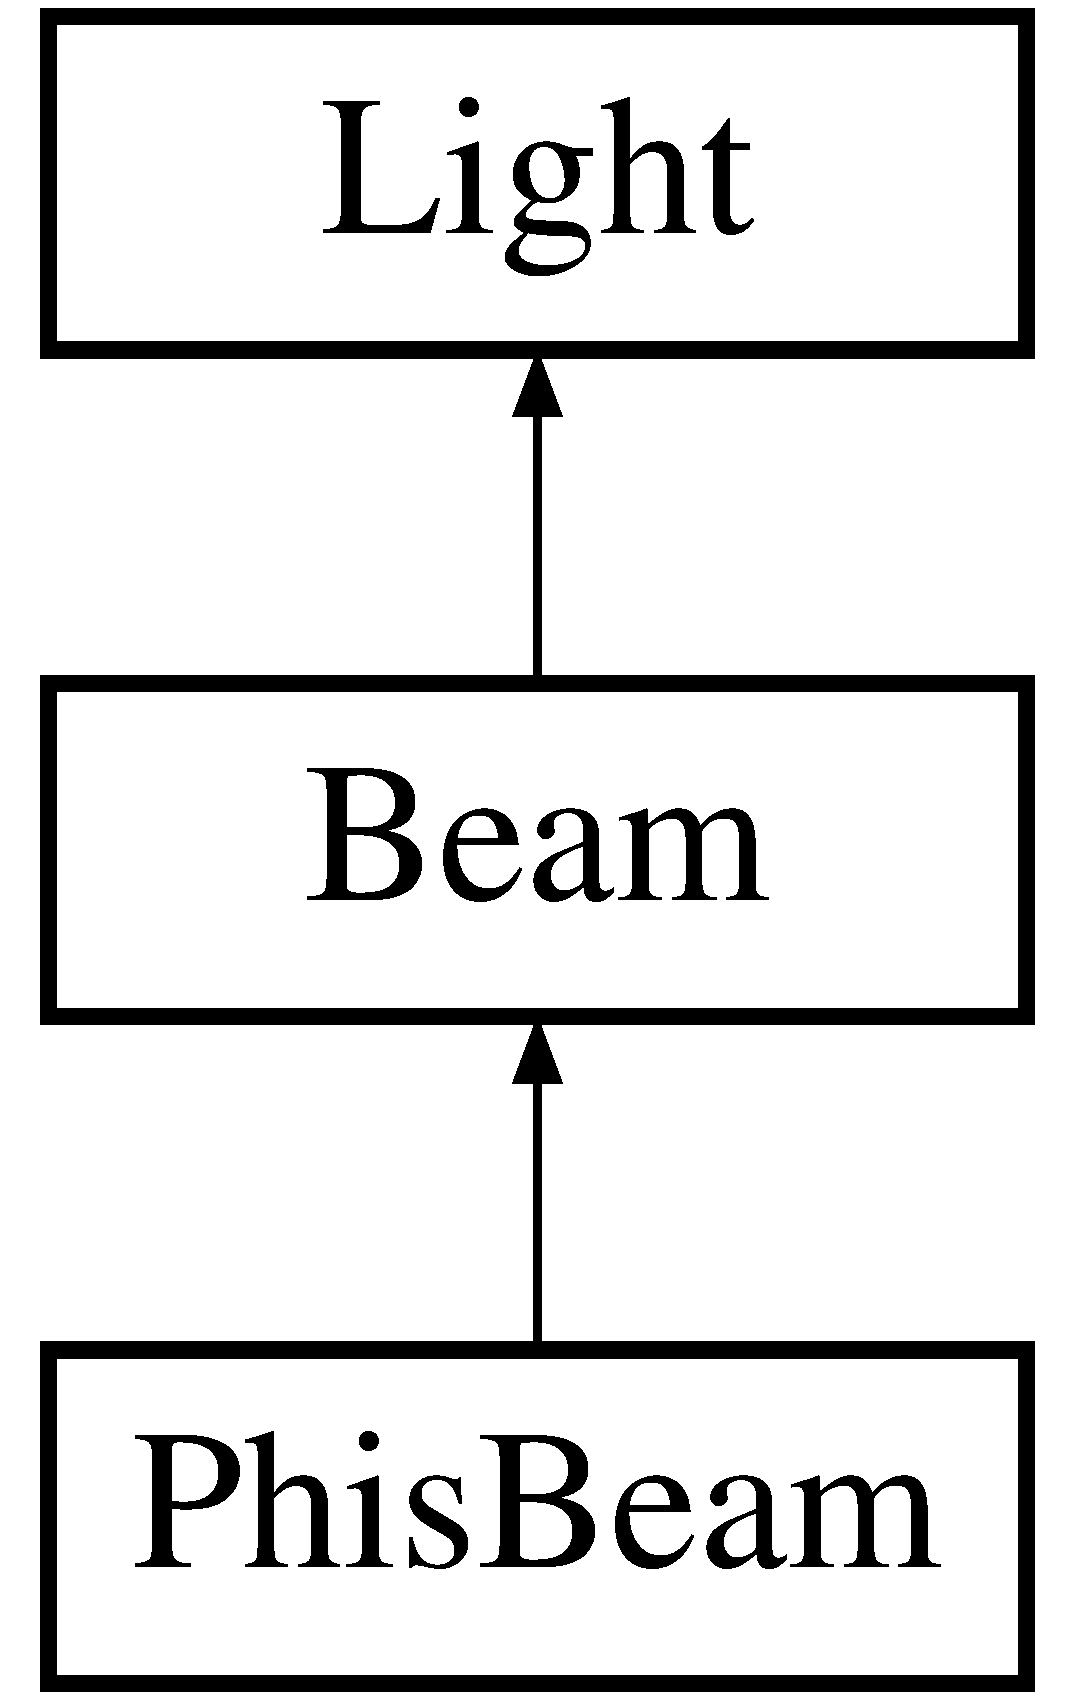
\includegraphics[height=3.000000cm]{class_light}
\end{center}
\end{figure}
\subsection*{Public Attributes}
\begin{DoxyCompactItemize}
\item 
\mbox{\Hypertarget{class_light_a91da59909da262125f2666e021540d91}\label{class_light_a91da59909da262125f2666e021540d91}} 
\mbox{\hyperlink{struct_point3f}{Point3f}} {\bfseries direction}
\item 
\mbox{\Hypertarget{class_light_a7a8f39612eb3949f754817a5fe843ac5}\label{class_light_a7a8f39612eb3949f754817a5fe843ac5}} 
\mbox{\hyperlink{struct_point3f}{Point3f}} {\bfseries polarization\+Basis}
\end{DoxyCompactItemize}


The documentation for this class was generated from the following file\+:\begin{DoxyCompactItemize}
\item 
common/Beam.\+h\end{DoxyCompactItemize}

\hypertarget{struct_clipper_lib_1_1_local_minimum}{}\section{Clipper\+Lib\+:\+:Local\+Minimum Struct Reference}
\label{struct_clipper_lib_1_1_local_minimum}\index{Clipper\+Lib\+::\+Local\+Minimum@{Clipper\+Lib\+::\+Local\+Minimum}}
\subsection*{Public Attributes}
\begin{DoxyCompactItemize}
\item 
\mbox{\Hypertarget{struct_clipper_lib_1_1_local_minimum_a71836a7c572ddfcf8853accb7314b7cf}\label{struct_clipper_lib_1_1_local_minimum_a71836a7c572ddfcf8853accb7314b7cf}} 
c\+Int {\bfseries Y}
\item 
\mbox{\Hypertarget{struct_clipper_lib_1_1_local_minimum_a0e7b997adca472b6e80f3223c45965ea}\label{struct_clipper_lib_1_1_local_minimum_a0e7b997adca472b6e80f3223c45965ea}} 
\mbox{\hyperlink{struct_clipper_lib_1_1_t_edge}{T\+Edge}} $\ast$ {\bfseries Left\+Bound}
\item 
\mbox{\Hypertarget{struct_clipper_lib_1_1_local_minimum_ade212cfb8c35da168b2bf20ad3e0ac94}\label{struct_clipper_lib_1_1_local_minimum_ade212cfb8c35da168b2bf20ad3e0ac94}} 
\mbox{\hyperlink{struct_clipper_lib_1_1_t_edge}{T\+Edge}} $\ast$ {\bfseries Right\+Bound}
\end{DoxyCompactItemize}


The documentation for this struct was generated from the following file\+:\begin{DoxyCompactItemize}
\item 
geometry/clipper/clipper.\+cpp\end{DoxyCompactItemize}

\hypertarget{struct_clipper_lib_1_1_loc_min_sorter}{}\section{Clipper\+Lib\+:\+:Loc\+Min\+Sorter Struct Reference}
\label{struct_clipper_lib_1_1_loc_min_sorter}\index{Clipper\+Lib\+::\+Loc\+Min\+Sorter@{Clipper\+Lib\+::\+Loc\+Min\+Sorter}}
\subsection*{Public Member Functions}
\begin{DoxyCompactItemize}
\item 
\mbox{\Hypertarget{struct_clipper_lib_1_1_loc_min_sorter_a4e5cd20cdd73b95700e91e61a8de5c06}\label{struct_clipper_lib_1_1_loc_min_sorter_a4e5cd20cdd73b95700e91e61a8de5c06}} 
bool {\bfseries operator()} (const \mbox{\hyperlink{struct_clipper_lib_1_1_local_minimum}{Local\+Minimum}} \&loc\+Min1, const \mbox{\hyperlink{struct_clipper_lib_1_1_local_minimum}{Local\+Minimum}} \&loc\+Min2)
\end{DoxyCompactItemize}


The documentation for this struct was generated from the following file\+:\begin{DoxyCompactItemize}
\item 
geometry/clipper/clipper.\+cpp\end{DoxyCompactItemize}

\hypertarget{classmatrix}{}\section{matrix Class Reference}
\label{classmatrix}\index{matrix@{matrix}}


The array with (n-\/rows x m-\/columns) dimensions of {\bfseries real} values. \mbox{\hyperlink{struct_size}{Size}} of the array can\textquotesingle{}t be changed.  




{\ttfamily \#include $<$matrix.\+hpp$>$}

\subsection*{Public Member Functions}
\begin{DoxyCompactItemize}
\item 
\mbox{\Hypertarget{classmatrix_add3506596457db2aa2b913bb9c364e31}\label{classmatrix_add3506596457db2aa2b913bb9c364e31}} 
\mbox{\hyperlink{classmatrix_add3506596457db2aa2b913bb9c364e31}{matrix}} (int \+\_\+n, int \+\_\+m)
\begin{DoxyCompactList}\small\item\em Creates and initializes new matrix. \end{DoxyCompactList}\item 
\mbox{\Hypertarget{classmatrix_a4018e1b43d9ce6fe0fe385e796b4ff9d}\label{classmatrix_a4018e1b43d9ce6fe0fe385e796b4ff9d}} 
{\bfseries matrix} (const \mbox{\hyperlink{classmatrix}{matrix}} \&)
\item 
\mbox{\Hypertarget{classmatrix_afe4d1e17fbbda7e391801eafbc951996}\label{classmatrix_afe4d1e17fbbda7e391801eafbc951996}} 
std\+::vector$<$ double $>$ {\bfseries To\+Vector} () const
\item 
\mbox{\Hypertarget{classmatrix_aa18ddf4f504206635586e48d7c2fbb68}\label{classmatrix_aa18ddf4f504206635586e48d7c2fbb68}} 
\mbox{\hyperlink{classmatrix}{matrix}} {\bfseries operator=} (const \mbox{\hyperlink{classmatrix}{matrix}} \&)
\item 
\mbox{\Hypertarget{classmatrix_a3ead8a54609a914a2b963a656d110282}\label{classmatrix_a3ead8a54609a914a2b963a656d110282}} 
\mbox{\hyperlink{classmatrix}{matrix}} {\bfseries operator+} (const \mbox{\hyperlink{classmatrix}{matrix}} \&) const
\item 
\mbox{\Hypertarget{classmatrix_a241b7864981d7886dd74f64e52cebbd0}\label{classmatrix_a241b7864981d7886dd74f64e52cebbd0}} 
\mbox{\hyperlink{classmatrix}{matrix}} {\bfseries operator+=} (const \mbox{\hyperlink{classmatrix}{matrix}} \&m)
\item 
\mbox{\Hypertarget{classmatrix_aefe9d9fce389bbbdf81a804a416dbe83}\label{classmatrix_aefe9d9fce389bbbdf81a804a416dbe83}} 
\mbox{\hyperlink{classmatrix}{matrix}} {\bfseries operator-\/} (const \mbox{\hyperlink{classmatrix}{matrix}} \&) const
\item 
\mbox{\Hypertarget{classmatrix_a445583c6509980c6aceeeebfb2fcd8e0}\label{classmatrix_a445583c6509980c6aceeeebfb2fcd8e0}} 
\mbox{\hyperlink{classmatrix}{matrix}} {\bfseries operator-\/=} (const \mbox{\hyperlink{classmatrix}{matrix}} \&m)
\item 
\mbox{\Hypertarget{classmatrix_a1ee2533474ec9e3b7db4203b8fb9b6e0}\label{classmatrix_a1ee2533474ec9e3b7db4203b8fb9b6e0}} 
double $\ast$ \mbox{\hyperlink{classmatrix_a1ee2533474ec9e3b7db4203b8fb9b6e0}{operator\mbox{[}$\,$\mbox{]}}} (int i) const
\begin{DoxyCompactList}\small\item\em The operator returns a pointer to the i-\/th row of the array. \end{DoxyCompactList}\item 
\mbox{\Hypertarget{classmatrix_a59139bc18f039339e9a581c96fddb674}\label{classmatrix_a59139bc18f039339e9a581c96fddb674}} 
\mbox{\hyperlink{classmatrix}{matrix}} {\bfseries operator$\ast$} (double) const
\item 
\mbox{\Hypertarget{classmatrix_a1b07b334ce71db5a644affa22bbb2ac2}\label{classmatrix_a1b07b334ce71db5a644affa22bbb2ac2}} 
\mbox{\hyperlink{classmatrix}{matrix}} {\bfseries operator$\ast$} (const \mbox{\hyperlink{classmatrix}{matrix}} \&) const
\item 
\mbox{\Hypertarget{classmatrix_aa29824e63e29bb6249db2076fcb20b9c}\label{classmatrix_aa29824e63e29bb6249db2076fcb20b9c}} 
\mbox{\hyperlink{classmatrix}{matrix}} {\bfseries operator$\ast$=} (double)
\item 
\mbox{\Hypertarget{classmatrix_a0a6164b6e48bae9ada50c8f4a5a68a22}\label{classmatrix_a0a6164b6e48bae9ada50c8f4a5a68a22}} 
\mbox{\hyperlink{classmatrix}{matrix}} {\bfseries operator/} (double) const
\item 
\mbox{\Hypertarget{classmatrix_ac3e138b950721c43de696919f7837978}\label{classmatrix_ac3e138b950721c43de696919f7837978}} 
\mbox{\hyperlink{classmatrix}{matrix}} {\bfseries operator/=} (double x)
\item 
\mbox{\Hypertarget{classmatrix_a6a864a6d8d0ff7f66c9bfd60a5fab5a4}\label{classmatrix_a6a864a6d8d0ff7f66c9bfd60a5fab5a4}} 
bool {\bfseries operator==} (const \mbox{\hyperlink{classmatrix}{matrix}} \&) const
\item 
\mbox{\Hypertarget{classmatrix_a9e37d73f37a3041272675c7c5d4b6782}\label{classmatrix_a9e37d73f37a3041272675c7c5d4b6782}} 
bool {\bfseries operator!=} (const \mbox{\hyperlink{classmatrix}{matrix}} \&m) const
\item 
\mbox{\Hypertarget{classmatrix_a2c882f692bfbca08d6f093a871a3fc7b}\label{classmatrix_a2c882f692bfbca08d6f093a871a3fc7b}} 
bool \mbox{\hyperlink{classmatrix_a2c882f692bfbca08d6f093a871a3fc7b}{is\+Square}} (void) const
\begin{DoxyCompactList}\small\item\em The function checks if the dimensions of the array are equal (n==m). \end{DoxyCompactList}\item 
\mbox{\Hypertarget{classmatrix_a317b8bf6d740cabf51ab9fd803e62a2c}\label{classmatrix_a317b8bf6d740cabf51ab9fd803e62a2c}} 
void \mbox{\hyperlink{classmatrix_a317b8bf6d740cabf51ab9fd803e62a2c}{Fill}} (double x)
\begin{DoxyCompactList}\small\item\em The function sets all values of the array to x. \end{DoxyCompactList}\item 
\mbox{\Hypertarget{classmatrix_a6f3af10a8808eebe72f1c41da20404f0}\label{classmatrix_a6f3af10a8808eebe72f1c41da20404f0}} 
void \mbox{\hyperlink{classmatrix_a6f3af10a8808eebe72f1c41da20404f0}{Identity}} (void)
\begin{DoxyCompactList}\small\item\em The function sets all the elements of the principal diagonal to one and all other elements to zero. The function do not check if the matrix is square. \end{DoxyCompactList}\item 
\mbox{\Hypertarget{classmatrix_aa24c1fbce7909df96d09ba75174f5859}\label{classmatrix_aa24c1fbce7909df96d09ba75174f5859}} 
void \mbox{\hyperlink{classmatrix_aa24c1fbce7909df96d09ba75174f5859}{Exchange}} (int i, int j)
\begin{DoxyCompactList}\small\item\em The function exchanges two rows. \end{DoxyCompactList}\item 
\mbox{\Hypertarget{classmatrix_aeb1dcd693cd6d18b731a2177f722eb6a}\label{classmatrix_aeb1dcd693cd6d18b731a2177f722eb6a}} 
int {\bfseries getN} () const
\item 
\mbox{\Hypertarget{classmatrix_a5f3532e4269da537bcb0a1377c49c2da}\label{classmatrix_a5f3532e4269da537bcb0a1377c49c2da}} 
int {\bfseries getM} () const
\end{DoxyCompactItemize}
\subsection*{Friends}
\begin{DoxyCompactItemize}
\item 
\mbox{\Hypertarget{classmatrix_a0f99416a4edc54f3db2dd8c5f7d546c5}\label{classmatrix_a0f99416a4edc54f3db2dd8c5f7d546c5}} 
\mbox{\hyperlink{classmatrix}{matrix}} {\bfseries operator$\ast$} (double x, const \mbox{\hyperlink{classmatrix}{matrix}} \&m)
\item 
\mbox{\Hypertarget{classmatrix_a488a52731e335f04938b08f64a776f67}\label{classmatrix_a488a52731e335f04938b08f64a776f67}} 
double \mbox{\hyperlink{classmatrix_a488a52731e335f04938b08f64a776f67}{norm}} (const \mbox{\hyperlink{classmatrix}{matrix}} \&)
\begin{DoxyCompactList}\small\item\em The function returns a sum of squares of all elements. \end{DoxyCompactList}\item 
\mbox{\Hypertarget{classmatrix_afead99146c1b79688d6609bb2b061808}\label{classmatrix_afead99146c1b79688d6609bb2b061808}} 
double \mbox{\hyperlink{classmatrix_afead99146c1b79688d6609bb2b061808}{Max}} (const \mbox{\hyperlink{classmatrix}{matrix}} \&)
\begin{DoxyCompactList}\small\item\em The function returns the square of maximal value of the array. \end{DoxyCompactList}\item 
int \mbox{\hyperlink{classmatrix_a55ecd7691eca1e7dac81020e9bd69038}{Str}} (const \mbox{\hyperlink{classmatrix}{matrix}} \&m)
\begin{DoxyCompactList}\small\item\em The function returns row counts. \end{DoxyCompactList}\item 
int \mbox{\hyperlink{classmatrix_a54850708093c314282f7f9c8162a493b}{Col}} (const \mbox{\hyperlink{classmatrix}{matrix}} \&m)
\begin{DoxyCompactList}\small\item\em The function returns column counts. \end{DoxyCompactList}\item 
\mbox{\Hypertarget{classmatrix_afadd635c5216a55b00380d8374c7eeac}\label{classmatrix_afadd635c5216a55b00380d8374c7eeac}} 
std\+::ofstream \& \mbox{\hyperlink{classmatrix_afadd635c5216a55b00380d8374c7eeac}{operator$<$$<$}} (std\+::ofstream \&, const \mbox{\hyperlink{classmatrix}{matrix}} \&)
\begin{DoxyCompactList}\small\item\em The operator outputs all elements of the array to the file separated by space. \end{DoxyCompactList}\end{DoxyCompactItemize}


\subsection{Detailed Description}
The array with (n-\/rows x m-\/columns) dimensions of {\bfseries real} values. \mbox{\hyperlink{struct_size}{Size}} of the array can\textquotesingle{}t be changed. 

\subsection{Friends And Related Function Documentation}
\mbox{\Hypertarget{classmatrix_a54850708093c314282f7f9c8162a493b}\label{classmatrix_a54850708093c314282f7f9c8162a493b}} 
\index{matrix@{matrix}!Col@{Col}}
\index{Col@{Col}!matrix@{matrix}}
\subsubsection{\texorpdfstring{Col}{Col}}
{\footnotesize\ttfamily int Col (\begin{DoxyParamCaption}\item[{const \mbox{\hyperlink{classmatrix}{matrix}} \&}]{m }\end{DoxyParamCaption})\hspace{0.3cm}{\ttfamily [friend]}}



The function returns column counts. 


\begin{DoxyParams}{Parameters}
{\em m} & the array \\
\hline
\end{DoxyParams}
\begin{DoxyReturn}{Returns}
row counts, (m.\+m) 
\end{DoxyReturn}
\mbox{\Hypertarget{classmatrix_a55ecd7691eca1e7dac81020e9bd69038}\label{classmatrix_a55ecd7691eca1e7dac81020e9bd69038}} 
\index{matrix@{matrix}!Str@{Str}}
\index{Str@{Str}!matrix@{matrix}}
\subsubsection{\texorpdfstring{Str}{Str}}
{\footnotesize\ttfamily int Str (\begin{DoxyParamCaption}\item[{const \mbox{\hyperlink{classmatrix}{matrix}} \&}]{m }\end{DoxyParamCaption})\hspace{0.3cm}{\ttfamily [friend]}}



The function returns row counts. 


\begin{DoxyParams}{Parameters}
{\em m} & the array \\
\hline
\end{DoxyParams}
\begin{DoxyReturn}{Returns}
row counts, (m.\+n) 
\end{DoxyReturn}


The documentation for this class was generated from the following files\+:\begin{DoxyCompactItemize}
\item 
math/matrix.\+hpp\item 
math/matrix.\+cpp\end{DoxyCompactItemize}

\hypertarget{class_matrix2x2c}{}\section{Matrix2x2c Class Reference}
\label{class_matrix2x2c}\index{Matrix2x2c@{Matrix2x2c}}


The \mbox{\hyperlink{class_matrix2x2c}{Matrix2x2c}} class Squad matrix with 4 complex elements (2x2)  




{\ttfamily \#include $<$Jones\+Matrix.\+h$>$}



Collaboration diagram for Matrix2x2c\+:
% FIG 0
\subsection*{Public Member Functions}
\begin{DoxyCompactItemize}
\item 
\mbox{\Hypertarget{class_matrix2x2c_a45a07c0462511e7ff00dab1a0246954d}\label{class_matrix2x2c_a45a07c0462511e7ff00dab1a0246954d}} 
{\bfseries Matrix2x2c} (const \mbox{\hyperlink{classmatrix_c}{matrixC}} \&m)
\item 
\mbox{\Hypertarget{class_matrix2x2c_a08a3e514022273afbb9602d97859d5e1}\label{class_matrix2x2c_a08a3e514022273afbb9602d97859d5e1}} 
double {\bfseries Norm} () const
\item 
\mbox{\Hypertarget{class_matrix2x2c_a695ab24fce73ea8731478bff19350de2}\label{class_matrix2x2c_a695ab24fce73ea8731478bff19350de2}} 
void {\bfseries Fill} (const \mbox{\hyperlink{classcomplex}{complex}} \&value)
\item 
\mbox{\Hypertarget{class_matrix2x2c_a980963d20e47533c17ffcd714d19681c}\label{class_matrix2x2c_a980963d20e47533c17ffcd714d19681c}} 
\mbox{\hyperlink{classmatrix_c}{matrixC}} {\bfseries operator$\ast$} (const \mbox{\hyperlink{classcomplex}{complex}} \&value) const
\item 
\mbox{\Hypertarget{class_matrix2x2c_a72183df24e5d34ff97e91fa879cdbd1b}\label{class_matrix2x2c_a72183df24e5d34ff97e91fa879cdbd1b}} 
\mbox{\hyperlink{class_matrix2x2c}{Matrix2x2c}} \& {\bfseries operator$\ast$=} (const double \&value)
\item 
\mbox{\Hypertarget{class_matrix2x2c_a70b6828f6137a2a1ac6dd07a074f717e}\label{class_matrix2x2c_a70b6828f6137a2a1ac6dd07a074f717e}} 
\mbox{\hyperlink{class_matrix2x2c}{Matrix2x2c}} \& {\bfseries operator+=} (const \mbox{\hyperlink{class_matrix2x2c}{Matrix2x2c}} \&other)
\end{DoxyCompactItemize}
\subsection*{Public Attributes}
\begin{DoxyCompactItemize}
\item 
\mbox{\Hypertarget{class_matrix2x2c_af410b74e0a6b338d06a596bdcc2f677e}\label{class_matrix2x2c_af410b74e0a6b338d06a596bdcc2f677e}} 
\mbox{\hyperlink{classcomplex}{complex}} {\bfseries m11}
\item 
\mbox{\Hypertarget{class_matrix2x2c_a4c14c07761d2cb5175c440c242f9c652}\label{class_matrix2x2c_a4c14c07761d2cb5175c440c242f9c652}} 
\mbox{\hyperlink{classcomplex}{complex}} {\bfseries m12}
\item 
\mbox{\Hypertarget{class_matrix2x2c_a37d76148fdb38b45181214d331729cd9}\label{class_matrix2x2c_a37d76148fdb38b45181214d331729cd9}} 
\mbox{\hyperlink{classcomplex}{complex}} {\bfseries m21}
\item 
\mbox{\Hypertarget{class_matrix2x2c_a350914905c4f7c29ae86f0c299fabc22}\label{class_matrix2x2c_a350914905c4f7c29ae86f0c299fabc22}} 
\mbox{\hyperlink{classcomplex}{complex}} {\bfseries m22}
\end{DoxyCompactItemize}


\subsection{Detailed Description}
The \mbox{\hyperlink{class_matrix2x2c}{Matrix2x2c}} class Squad matrix with 4 complex elements (2x2) 

The documentation for this class was generated from the following files\+:\begin{DoxyCompactItemize}
\item 
math/Jones\+Matrix.\+h\item 
math/Jones\+Matrix.\+cpp\end{DoxyCompactItemize}

\hypertarget{class_matrix4x4d}{}\section{Matrix4x4d Class Reference}
\label{class_matrix4x4d}\index{Matrix4x4d@{Matrix4x4d}}


Inheritance diagram for Matrix4x4d\+:
% FIG 0
\subsection*{Public Member Functions}
\begin{DoxyCompactItemize}
\item 
\mbox{\Hypertarget{class_matrix4x4d_a9f8882b7cf03d260103d5e9ffd2ff6fb}\label{class_matrix4x4d_a9f8882b7cf03d260103d5e9ffd2ff6fb}} 
void {\bfseries Reset} ()
\item 
\mbox{\Hypertarget{class_matrix4x4d_a8c6221d46f27a0f9f7ad1b65f7de7085}\label{class_matrix4x4d_a8c6221d46f27a0f9f7ad1b65f7de7085}} 
\mbox{\hyperlink{class_matrix4x4d}{Matrix4x4d}} {\bfseries operator-\/} (const \mbox{\hyperlink{class_matrix4x4d}{Matrix4x4d}} \&other) const
\item 
\mbox{\Hypertarget{class_matrix4x4d_ac2a63d675429cae482db92c165a5a23b}\label{class_matrix4x4d_ac2a63d675429cae482db92c165a5a23b}} 
void {\bfseries operator+=} (const \mbox{\hyperlink{class_matrix4x4d}{Matrix4x4d}} \&other)
\item 
\mbox{\Hypertarget{class_matrix4x4d_a42a09732f017713333e8bce2a0ef649c}\label{class_matrix4x4d_a42a09732f017713333e8bce2a0ef649c}} 
void {\bfseries operator$\ast$=} (double value)
\item 
\mbox{\Hypertarget{class_matrix4x4d_a86228dbd8264f212ead840165add0089}\label{class_matrix4x4d_a86228dbd8264f212ead840165add0089}} 
double {\bfseries operator()} (int i, int j) const
\item 
\mbox{\Hypertarget{class_matrix4x4d_acae8b73e02a1878a08d97deceed333bf}\label{class_matrix4x4d_acae8b73e02a1878a08d97deceed333bf}} 
double \& {\bfseries operator()} (int i, int j)
\end{DoxyCompactItemize}
\subsection*{Protected Attributes}
\begin{DoxyCompactItemize}
\item 
\mbox{\Hypertarget{class_matrix4x4d_a83e2bb6d4ae55d8438de553a4716ac06}\label{class_matrix4x4d_a83e2bb6d4ae55d8438de553a4716ac06}} 
double {\bfseries m\+\_\+array} \mbox{[}M\+X\+\_\+\+R\+A\+NK\mbox{]}\mbox{[}M\+X\+\_\+\+R\+A\+NK\mbox{]}
\end{DoxyCompactItemize}
\subsection*{Friends}
\begin{DoxyCompactItemize}
\item 
\mbox{\Hypertarget{class_matrix4x4d_a95e0e03428f4cf3315e0666ed529cb27}\label{class_matrix4x4d_a95e0e03428f4cf3315e0666ed529cb27}} 
std\+::ofstream \& {\bfseries operator$<$$<$} (std\+::ofstream \&out, const \mbox{\hyperlink{class_matrix4x4d}{Matrix4x4d}} \&m)
\end{DoxyCompactItemize}


The documentation for this class was generated from the following files\+:\begin{DoxyCompactItemize}
\item 
common/Matrix4x4.\+h\item 
common/Matrix4x4.\+cpp\end{DoxyCompactItemize}

\hypertarget{classmatrix_c}{}\section{matrixC Class Reference}
\label{classmatrix_c}\index{matrixC@{matrixC}}


The array with (n-\/rows x m-\/columns) dimensions of {\bfseries complex} values. \mbox{\hyperlink{struct_size}{Size}} of the array can\textquotesingle{}t be changed.  




{\ttfamily \#include $<$matrix.\+hpp$>$}

\subsection*{Public Member Functions}
\begin{DoxyCompactItemize}
\item 
\mbox{\Hypertarget{classmatrix_c_af6a11558b8cecaa782216065efc9779e}\label{classmatrix_c_af6a11558b8cecaa782216065efc9779e}} 
\mbox{\hyperlink{classmatrix_c_af6a11558b8cecaa782216065efc9779e}{matrixC}} (int \+\_\+n, int \+\_\+m)
\begin{DoxyCompactList}\small\item\em Creates and initializes new matrix. \end{DoxyCompactList}\item 
\mbox{\Hypertarget{classmatrix_c_a192c20453e6d7feec6566789e740fa41}\label{classmatrix_c_a192c20453e6d7feec6566789e740fa41}} 
{\bfseries matrixC} (const \mbox{\hyperlink{classmatrix_c}{matrixC}} \&)
\item 
\mbox{\Hypertarget{classmatrix_c_ac0bbe7cec74175a4b33d9c4695f09c38}\label{classmatrix_c_ac0bbe7cec74175a4b33d9c4695f09c38}} 
\mbox{\hyperlink{classmatrix_c}{matrixC}} {\bfseries operator=} (const \mbox{\hyperlink{classmatrix_c}{matrixC}} \&)
\item 
\mbox{\Hypertarget{classmatrix_c_a54eb9c60036ded09ba24edc0f561abcc}\label{classmatrix_c_a54eb9c60036ded09ba24edc0f561abcc}} 
\mbox{\hyperlink{classmatrix_c}{matrixC}} {\bfseries operator+} (const \mbox{\hyperlink{classmatrix_c}{matrixC}} \&) const
\item 
\mbox{\Hypertarget{classmatrix_c_a033b3655af1c81c08cfb0d065a871dcc}\label{classmatrix_c_a033b3655af1c81c08cfb0d065a871dcc}} 
\mbox{\hyperlink{classmatrix_c}{matrixC}} {\bfseries operator+=} (const \mbox{\hyperlink{classmatrix_c}{matrixC}} \&m)
\item 
\mbox{\Hypertarget{classmatrix_c_a91586bd1a69f33e5d1b248bd7a96e3c0}\label{classmatrix_c_a91586bd1a69f33e5d1b248bd7a96e3c0}} 
\mbox{\hyperlink{classmatrix_c}{matrixC}} {\bfseries operator-\/} (const \mbox{\hyperlink{classmatrix_c}{matrixC}} \&) const
\item 
\mbox{\Hypertarget{classmatrix_c_a03fd46edf995a822b88fbd99394e4e31}\label{classmatrix_c_a03fd46edf995a822b88fbd99394e4e31}} 
\mbox{\hyperlink{classmatrix_c}{matrixC}} {\bfseries operator-\/=} (const \mbox{\hyperlink{classmatrix_c}{matrixC}} \&m)
\item 
\mbox{\Hypertarget{classmatrix_c_a48d4698231c0a122f045e0bd816b4897}\label{classmatrix_c_a48d4698231c0a122f045e0bd816b4897}} 
\mbox{\hyperlink{classcomplex}{complex}} $\ast$ \mbox{\hyperlink{classmatrix_c_a48d4698231c0a122f045e0bd816b4897}{operator\mbox{[}$\,$\mbox{]}}} (int N) const
\begin{DoxyCompactList}\small\item\em The operator returns a pointer to the i-\/th row of the array. \end{DoxyCompactList}\item 
\mbox{\Hypertarget{classmatrix_c_ac634dc38aa8b680be06bec32409cca2c}\label{classmatrix_c_ac634dc38aa8b680be06bec32409cca2c}} 
\mbox{\hyperlink{classmatrix_c}{matrixC}} {\bfseries operator$\ast$} (const \mbox{\hyperlink{classcomplex}{complex}} \&) const
\item 
\mbox{\Hypertarget{classmatrix_c_a2494dc4fde03bf506991f19f2fce6de8}\label{classmatrix_c_a2494dc4fde03bf506991f19f2fce6de8}} 
\mbox{\hyperlink{classmatrix_c}{matrixC}} {\bfseries operator$\ast$} (const \mbox{\hyperlink{classmatrix}{matrix}} \&) const
\item 
\mbox{\Hypertarget{classmatrix_c_a522859445d59f2eff1865665ac57621c}\label{classmatrix_c_a522859445d59f2eff1865665ac57621c}} 
\mbox{\hyperlink{classmatrix_c}{matrixC}} {\bfseries operator$\ast$} (const \mbox{\hyperlink{classmatrix_c}{matrixC}} \&) const
\item 
\mbox{\Hypertarget{classmatrix_c_aabc813e1e376d8918cec2cc8eb10b33f}\label{classmatrix_c_aabc813e1e376d8918cec2cc8eb10b33f}} 
\mbox{\hyperlink{classmatrix_c}{matrixC}} {\bfseries operator$\ast$=} (const \mbox{\hyperlink{classcomplex}{complex}} \&z)
\item 
\mbox{\Hypertarget{classmatrix_c_aba9937224522c2873ab26377b4ea8d71}\label{classmatrix_c_aba9937224522c2873ab26377b4ea8d71}} 
\mbox{\hyperlink{classmatrix_c}{matrixC}} {\bfseries operator/} (const \mbox{\hyperlink{classcomplex}{complex}} \&) const
\item 
\mbox{\Hypertarget{classmatrix_c_ab8b0021504bde91ff5af3ba6a81e049e}\label{classmatrix_c_ab8b0021504bde91ff5af3ba6a81e049e}} 
\mbox{\hyperlink{classmatrix_c}{matrixC}} {\bfseries operator/=} (const \mbox{\hyperlink{classcomplex}{complex}} \&)
\item 
\mbox{\Hypertarget{classmatrix_c_afea62d5f6f4e300fccce98118d61532d}\label{classmatrix_c_afea62d5f6f4e300fccce98118d61532d}} 
bool {\bfseries operator==} (const \mbox{\hyperlink{classmatrix_c}{matrixC}} \&) const
\item 
\mbox{\Hypertarget{classmatrix_c_abf75721e3eec535988ae0b2d49905751}\label{classmatrix_c_abf75721e3eec535988ae0b2d49905751}} 
bool {\bfseries operator!=} (const \mbox{\hyperlink{classmatrix_c}{matrixC}} \&m) const
\item 
\mbox{\Hypertarget{classmatrix_c_ac5261695dffb2b3baf6f03da1d32d5eb}\label{classmatrix_c_ac5261695dffb2b3baf6f03da1d32d5eb}} 
void \mbox{\hyperlink{classmatrix_c_ac5261695dffb2b3baf6f03da1d32d5eb}{Fill}} (const \mbox{\hyperlink{classcomplex}{complex}} \&z)
\begin{DoxyCompactList}\small\item\em The function sets all values of the array to z. \end{DoxyCompactList}\item 
\mbox{\Hypertarget{classmatrix_c_a521f6a7fff5de8401e194d99f75ef179}\label{classmatrix_c_a521f6a7fff5de8401e194d99f75ef179}} 
void \mbox{\hyperlink{classmatrix_c_a521f6a7fff5de8401e194d99f75ef179}{Identity}} (void)
\begin{DoxyCompactList}\small\item\em The function sets all the elements of the principal diagonal to one and all other elements to zero. The function do not check if the matrix is square. \end{DoxyCompactList}\item 
\mbox{\Hypertarget{classmatrix_c_a7ed75aec8114e3ceaa890a8f2aed21e2}\label{classmatrix_c_a7ed75aec8114e3ceaa890a8f2aed21e2}} 
void \mbox{\hyperlink{classmatrix_c_a7ed75aec8114e3ceaa890a8f2aed21e2}{Exchange}} (int i, int j)
\begin{DoxyCompactList}\small\item\em The function exchanges two rows. \end{DoxyCompactList}\end{DoxyCompactItemize}
\subsection*{Friends}
\begin{DoxyCompactItemize}
\item 
\mbox{\Hypertarget{classmatrix_c_acae2edb23217265c061f306c52912c19}\label{classmatrix_c_acae2edb23217265c061f306c52912c19}} 
double \mbox{\hyperlink{classmatrix_c_acae2edb23217265c061f306c52912c19}{norm}} (const \mbox{\hyperlink{classmatrix_c}{matrixC}} \&)
\begin{DoxyCompactList}\small\item\em The function returns a sum of squares of all elements. \end{DoxyCompactList}\item 
\mbox{\Hypertarget{classmatrix_c_ac39f0a59997bb6678063cebbdada2b82}\label{classmatrix_c_ac39f0a59997bb6678063cebbdada2b82}} 
double \mbox{\hyperlink{classmatrix_c_ac39f0a59997bb6678063cebbdada2b82}{Max}} (const \mbox{\hyperlink{classmatrix_c}{matrixC}} \&)
\begin{DoxyCompactList}\small\item\em The function returns the square of maximal value of the array. \end{DoxyCompactList}\item 
int \mbox{\hyperlink{classmatrix_c_a899bdb2aece2b65c6ef7b6fadf4a124b}{Str}} (const \mbox{\hyperlink{classmatrix_c}{matrixC}} \&m)
\begin{DoxyCompactList}\small\item\em The function returns row counts. \end{DoxyCompactList}\item 
int \mbox{\hyperlink{classmatrix_c_a760a278d008e2717135156531da1450b}{Col}} (const \mbox{\hyperlink{classmatrix_c}{matrixC}} \&m)
\begin{DoxyCompactList}\small\item\em The function returns column counts. \end{DoxyCompactList}\item 
\mbox{\Hypertarget{classmatrix_c_a65ec7d14c0de729285d48fa94749dcee}\label{classmatrix_c_a65ec7d14c0de729285d48fa94749dcee}} 
\mbox{\hyperlink{classmatrix_c}{matrixC}} {\bfseries operator$\ast$} (const \mbox{\hyperlink{classcomplex}{complex}} \&z, const \mbox{\hyperlink{classmatrix_c}{matrixC}} \&m)
\item 
\mbox{\Hypertarget{classmatrix_c_ab321eae7cb92218cffee53cfd151e167}\label{classmatrix_c_ab321eae7cb92218cffee53cfd151e167}} 
std\+::ofstream \& \mbox{\hyperlink{classmatrix_c_ab321eae7cb92218cffee53cfd151e167}{operator$<$$<$}} (std\+::ofstream \&, const \mbox{\hyperlink{classmatrix_c}{matrixC}} \&)
\begin{DoxyCompactList}\small\item\em The operator outputs all elements of the array to the file separated by space. Real and Imagen parts are separated by comma. \end{DoxyCompactList}\end{DoxyCompactItemize}


\subsection{Detailed Description}
The array with (n-\/rows x m-\/columns) dimensions of {\bfseries complex} values. \mbox{\hyperlink{struct_size}{Size}} of the array can\textquotesingle{}t be changed. 

\subsection{Friends And Related Function Documentation}
\mbox{\Hypertarget{classmatrix_c_a760a278d008e2717135156531da1450b}\label{classmatrix_c_a760a278d008e2717135156531da1450b}} 
\index{matrixC@{matrixC}!Col@{Col}}
\index{Col@{Col}!matrixC@{matrixC}}
\subsubsection{\texorpdfstring{Col}{Col}}
{\footnotesize\ttfamily int Col (\begin{DoxyParamCaption}\item[{const \mbox{\hyperlink{classmatrix_c}{matrixC}} \&}]{m }\end{DoxyParamCaption})\hspace{0.3cm}{\ttfamily [friend]}}



The function returns column counts. 


\begin{DoxyParams}{Parameters}
{\em m} & the array \\
\hline
\end{DoxyParams}
\begin{DoxyReturn}{Returns}
row counts, (m.\+m) 
\end{DoxyReturn}
\mbox{\Hypertarget{classmatrix_c_a899bdb2aece2b65c6ef7b6fadf4a124b}\label{classmatrix_c_a899bdb2aece2b65c6ef7b6fadf4a124b}} 
\index{matrixC@{matrixC}!Str@{Str}}
\index{Str@{Str}!matrixC@{matrixC}}
\subsubsection{\texorpdfstring{Str}{Str}}
{\footnotesize\ttfamily int Str (\begin{DoxyParamCaption}\item[{const \mbox{\hyperlink{classmatrix_c}{matrixC}} \&}]{m }\end{DoxyParamCaption})\hspace{0.3cm}{\ttfamily [friend]}}



The function returns row counts. 


\begin{DoxyParams}{Parameters}
{\em m} & the array \\
\hline
\end{DoxyParams}
\begin{DoxyReturn}{Returns}
row counts, (m.\+n) 
\end{DoxyReturn}


The documentation for this class was generated from the following files\+:\begin{DoxyCompactItemize}
\item 
math/matrix.\+hpp\item 
math/matrix.\+cpp\end{DoxyCompactItemize}

\hypertarget{class_mueller_matrix}{}\section{Mueller\+Matrix Class Reference}
\label{class_mueller_matrix}\index{Mueller\+Matrix@{Mueller\+Matrix}}


Inheritance diagram for Mueller\+Matrix\+:
% FIG 0


Collaboration diagram for Mueller\+Matrix\+:
% FIG 1
\subsection*{Public Member Functions}
\begin{DoxyCompactItemize}
\item 
\mbox{\Hypertarget{class_mueller_matrix_a567e0f446f455f3eec493029c2983dbb}\label{class_mueller_matrix_a567e0f446f455f3eec493029c2983dbb}} 
{\bfseries Mueller\+Matrix} (const \mbox{\hyperlink{class_matrix2x2c}{Matrix2x2c}} \&in)
\item 
\mbox{\Hypertarget{class_mueller_matrix_a13b75f898bb755242ef968cc7a680355}\label{class_mueller_matrix_a13b75f898bb755242ef968cc7a680355}} 
{\bfseries Mueller\+Matrix} (const \mbox{\hyperlink{classmatrix_c}{matrixC}} \&in)
\end{DoxyCompactItemize}
\subsection*{Additional Inherited Members}


The documentation for this class was generated from the following files\+:\begin{DoxyCompactItemize}
\item 
common/Muller\+Matrix.\+h\item 
common/Muller\+Matrix.\+cpp\end{DoxyCompactItemize}

\hypertarget{class_normal_incidence}{}\section{Normal\+Incidence Class Reference}
\label{class_normal_incidence}\index{Normal\+Incidence@{Normal\+Incidence}}
Inheritance diagram for Normal\+Incidence\+:\begin{figure}[H]
\begin{center}
\leavevmode
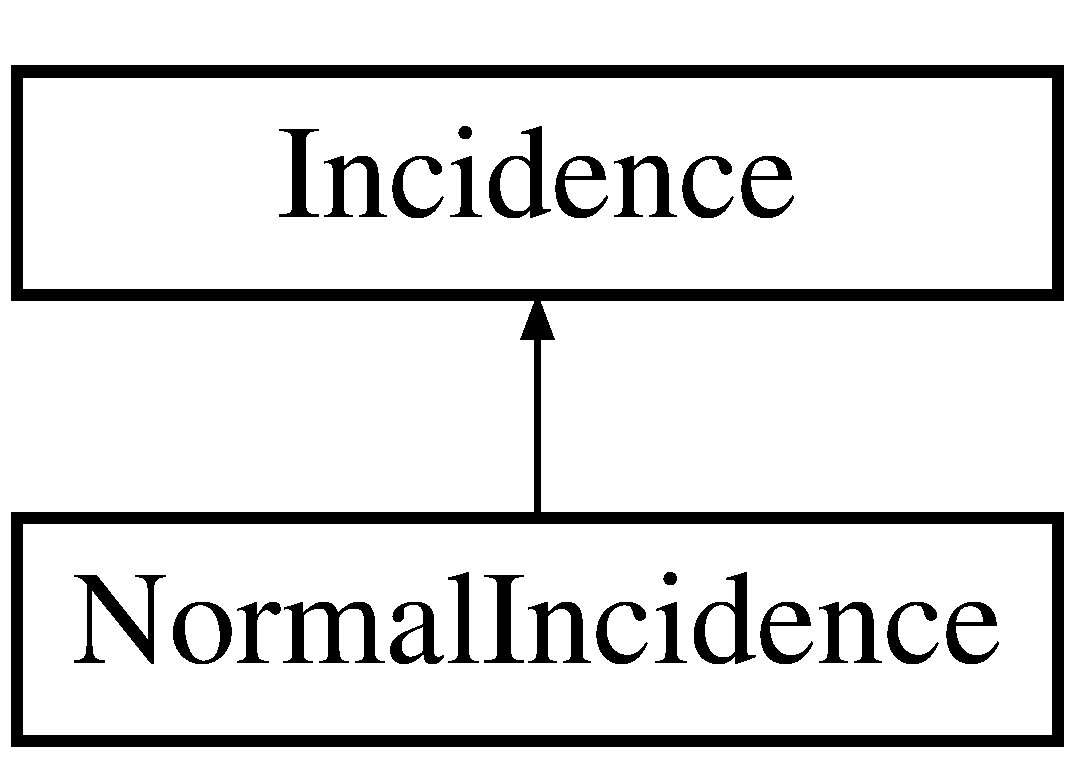
\includegraphics[height=2.000000cm]{class_normal_incidence}
\end{center}
\end{figure}
\subsection*{Public Member Functions}
\begin{DoxyCompactItemize}
\item 
\mbox{\Hypertarget{class_normal_incidence_a0e02aa34d04670aa431a88dcc6016c36}\label{class_normal_incidence_a0e02aa34d04670aa431a88dcc6016c36}} 
virtual void {\bfseries Compute\+Directions} (const \mbox{\hyperlink{class_beam}{Beam}} \&beam, \mbox{\hyperlink{class_splitting}{Splitting}} \&splitter) const override
\item 
\mbox{\Hypertarget{class_normal_incidence_acc09bec130f6d1dfea67afd729c41567}\label{class_normal_incidence_acc09bec130f6d1dfea67afd729c41567}} 
virtual void {\bfseries Compute\+Jones\+Matrices} (const \mbox{\hyperlink{class_beam}{Beam}} \&beam, \mbox{\hyperlink{class_splitting}{Splitting}} \&splitter) const override
\end{DoxyCompactItemize}


The documentation for this class was generated from the following files\+:\begin{DoxyCompactItemize}
\item 
incidence/Normal\+Incidence.\+h\item 
incidence/Normal\+Incidence.\+cpp\end{DoxyCompactItemize}

\hypertarget{class_numberlike_array}{}\section{Numberlike\+Array$<$ Blk $>$ Class Template Reference}
\label{class_numberlike_array}\index{Numberlike\+Array$<$ Blk $>$@{Numberlike\+Array$<$ Blk $>$}}


Collaboration diagram for Numberlike\+Array$<$ Blk $>$\+:
% FIG 0
\subsection*{Public Types}
\begin{DoxyCompactItemize}
\item 
\mbox{\Hypertarget{class_numberlike_array_a7ad8506727ac4e2f4c7850cc41f4142c}\label{class_numberlike_array_a7ad8506727ac4e2f4c7850cc41f4142c}} 
typedef unsigned int {\bfseries Index}
\end{DoxyCompactItemize}
\subsection*{Public Member Functions}
\begin{DoxyCompactItemize}
\item 
\mbox{\Hypertarget{class_numberlike_array_a787b3f19ed994ee9dc87613a052a51ca}\label{class_numberlike_array_a787b3f19ed994ee9dc87613a052a51ca}} 
{\bfseries Numberlike\+Array} (Index c)
\item 
\mbox{\Hypertarget{class_numberlike_array_af679905e09b95d7b0ae4174d473b25f8}\label{class_numberlike_array_af679905e09b95d7b0ae4174d473b25f8}} 
void {\bfseries allocate} (Index c)
\item 
\mbox{\Hypertarget{class_numberlike_array_af33c23327f2abe6850264180b3147055}\label{class_numberlike_array_af33c23327f2abe6850264180b3147055}} 
void {\bfseries allocate\+And\+Copy} (Index c)
\item 
\mbox{\Hypertarget{class_numberlike_array_aec3cb7d201b1db27d41b7722530e7b54}\label{class_numberlike_array_aec3cb7d201b1db27d41b7722530e7b54}} 
{\bfseries Numberlike\+Array} (const \mbox{\hyperlink{class_numberlike_array}{Numberlike\+Array}}$<$ Blk $>$ \&x)
\item 
\mbox{\Hypertarget{class_numberlike_array_a0c68894dfe11e7786b4768c7258bf4c6}\label{class_numberlike_array_a0c68894dfe11e7786b4768c7258bf4c6}} 
void {\bfseries operator=} (const \mbox{\hyperlink{class_numberlike_array}{Numberlike\+Array}}$<$ Blk $>$ \&x)
\item 
\mbox{\Hypertarget{class_numberlike_array_acd313b6f0036aada1dc5ef596101e934}\label{class_numberlike_array_acd313b6f0036aada1dc5ef596101e934}} 
{\bfseries Numberlike\+Array} (const Blk $\ast$b, Index blen)
\item 
\mbox{\Hypertarget{class_numberlike_array_ab4bf2e96e006c9237d3233e1f2f30add}\label{class_numberlike_array_ab4bf2e96e006c9237d3233e1f2f30add}} 
Index {\bfseries get\+Capacity} () const
\item 
\mbox{\Hypertarget{class_numberlike_array_a14eef564b220025975d95da51c3c33d7}\label{class_numberlike_array_a14eef564b220025975d95da51c3c33d7}} 
Index {\bfseries get\+Length} () const
\item 
\mbox{\Hypertarget{class_numberlike_array_a1eb37624f06f01b9fa1d794a71b0fa03}\label{class_numberlike_array_a1eb37624f06f01b9fa1d794a71b0fa03}} 
Blk {\bfseries get\+Block} (Index i) const
\item 
\mbox{\Hypertarget{class_numberlike_array_a10acd5b5c4c571a531019db373b6ffbf}\label{class_numberlike_array_a10acd5b5c4c571a531019db373b6ffbf}} 
bool {\bfseries is\+Empty} () const
\item 
\mbox{\Hypertarget{class_numberlike_array_ab8abf1847351e6b1aa5f18bc47bd3bd6}\label{class_numberlike_array_ab8abf1847351e6b1aa5f18bc47bd3bd6}} 
bool {\bfseries operator==} (const \mbox{\hyperlink{class_numberlike_array}{Numberlike\+Array}}$<$ Blk $>$ \&x) const
\item 
\mbox{\Hypertarget{class_numberlike_array_a015fd3cc55a9c0f37ec43cfd0348b3f2}\label{class_numberlike_array_a015fd3cc55a9c0f37ec43cfd0348b3f2}} 
bool {\bfseries operator!=} (const \mbox{\hyperlink{class_numberlike_array}{Numberlike\+Array}}$<$ Blk $>$ \&x) const
\end{DoxyCompactItemize}
\subsection*{Public Attributes}
\begin{DoxyCompactItemize}
\item 
\mbox{\Hypertarget{class_numberlike_array_ab1a4e9d5eda64625ab32054645e82489}\label{class_numberlike_array_ab1a4e9d5eda64625ab32054645e82489}} 
Index {\bfseries cap}
\item 
\mbox{\Hypertarget{class_numberlike_array_aa016f396175bd4084f40204a4d748eb9}\label{class_numberlike_array_aa016f396175bd4084f40204a4d748eb9}} 
Index {\bfseries len}
\item 
\mbox{\Hypertarget{class_numberlike_array_a378baefd25f016ba27ade9cc5dbb09b2}\label{class_numberlike_array_a378baefd25f016ba27ade9cc5dbb09b2}} 
Blk $\ast$ {\bfseries blk}
\end{DoxyCompactItemize}
\subsection*{Static Public Attributes}
\begin{DoxyCompactItemize}
\item 
\mbox{\Hypertarget{class_numberlike_array_a25b7418a31008a14a5efd6610b0fa258}\label{class_numberlike_array_a25b7418a31008a14a5efd6610b0fa258}} 
static const unsigned int {\bfseries N} = 8 $\ast$ sizeof(Blk)
\end{DoxyCompactItemize}


The documentation for this class was generated from the following file\+:\begin{DoxyCompactItemize}
\item 
bigint/Numberlike\+Array.\+hh\end{DoxyCompactItemize}

\hypertarget{struct_optical_path}{}\section{Optical\+Path Struct Reference}
\label{struct_optical_path}\index{Optical\+Path@{Optical\+Path}}
\subsection*{Public Member Functions}
\begin{DoxyCompactItemize}
\item 
\mbox{\Hypertarget{struct_optical_path_a387fb1a12b74bb1b1589f19e74b13af1}\label{struct_optical_path_a387fb1a12b74bb1b1589f19e74b13af1}} 
double {\bfseries Get\+Total} ()
\end{DoxyCompactItemize}
\subsection*{Public Attributes}
\begin{DoxyCompactItemize}
\item 
\mbox{\Hypertarget{struct_optical_path_af1521166cf4e510161ed127cdee12b82}\label{struct_optical_path_af1521166cf4e510161ed127cdee12b82}} 
double {\bfseries internal} = 0
\item 
\mbox{\Hypertarget{struct_optical_path_a4c8fa24427bf6641772fa9939c0eca77}\label{struct_optical_path_a4c8fa24427bf6641772fa9939c0eca77}} 
double {\bfseries external} = 0
\end{DoxyCompactItemize}


The documentation for this struct was generated from the following file\+:\begin{DoxyCompactItemize}
\item 
scattering/Scattering.\+h\end{DoxyCompactItemize}

\hypertarget{class_orientation}{}\section{Orientation Class Reference}
\label{class_orientation}\index{Orientation@{Orientation}}
\subsection*{Public Attributes}
\begin{DoxyCompactItemize}
\item 
\mbox{\Hypertarget{class_orientation_acffab8b9c7a0f6b4a5e24d049f736abe}\label{class_orientation_acffab8b9c7a0f6b4a5e24d049f736abe}} 
double {\bfseries beta}
\item 
\mbox{\Hypertarget{class_orientation_aa745459cdf332f9ad128d2194ce02f9d}\label{class_orientation_aa745459cdf332f9ad128d2194ce02f9d}} 
double {\bfseries gamma}
\item 
\mbox{\Hypertarget{class_orientation_a6c74f24ac48bd9fdbada2ae67860afe1}\label{class_orientation_a6c74f24ac48bd9fdbada2ae67860afe1}} 
double {\bfseries alpha}
\end{DoxyCompactItemize}


The documentation for this class was generated from the following file\+:\begin{DoxyCompactItemize}
\item 
geometry/geometry\+\_\+lib.\+h\end{DoxyCompactItemize}

\hypertarget{struct_clipper_lib_1_1_out_pt}{}\section{Clipper\+Lib\+:\+:Out\+Pt Struct Reference}
\label{struct_clipper_lib_1_1_out_pt}\index{Clipper\+Lib\+::\+Out\+Pt@{Clipper\+Lib\+::\+Out\+Pt}}
\subsection*{Public Attributes}
\begin{DoxyCompactItemize}
\item 
\mbox{\Hypertarget{struct_clipper_lib_1_1_out_pt_ad04d3691d47a5d0d9b2ae097e7e7bf10}\label{struct_clipper_lib_1_1_out_pt_ad04d3691d47a5d0d9b2ae097e7e7bf10}} 
int {\bfseries Idx}
\item 
\mbox{\Hypertarget{struct_clipper_lib_1_1_out_pt_aa01c2b1e9c5b2d8faa40701178ffcf98}\label{struct_clipper_lib_1_1_out_pt_aa01c2b1e9c5b2d8faa40701178ffcf98}} 
\mbox{\hyperlink{struct_clipper_lib_1_1_int_point}{Int\+Point}} {\bfseries Pt}
\item 
\mbox{\Hypertarget{struct_clipper_lib_1_1_out_pt_a2d605b87f6da37dbdbef990c4fa5819e}\label{struct_clipper_lib_1_1_out_pt_a2d605b87f6da37dbdbef990c4fa5819e}} 
\mbox{\hyperlink{struct_clipper_lib_1_1_out_pt}{Out\+Pt}} $\ast$ {\bfseries Next}
\item 
\mbox{\Hypertarget{struct_clipper_lib_1_1_out_pt_a609eb414d5764e78150cceccaffc5d54}\label{struct_clipper_lib_1_1_out_pt_a609eb414d5764e78150cceccaffc5d54}} 
\mbox{\hyperlink{struct_clipper_lib_1_1_out_pt}{Out\+Pt}} $\ast$ {\bfseries Prev}
\end{DoxyCompactItemize}


The documentation for this struct was generated from the following file\+:\begin{DoxyCompactItemize}
\item 
geometry/clipper/clipper.\+cpp\end{DoxyCompactItemize}

\hypertarget{struct_clipper_lib_1_1_out_rec}{}\section{Clipper\+Lib\+:\+:Out\+Rec Struct Reference}
\label{struct_clipper_lib_1_1_out_rec}\index{Clipper\+Lib\+::\+Out\+Rec@{Clipper\+Lib\+::\+Out\+Rec}}
\subsection*{Public Attributes}
\begin{DoxyCompactItemize}
\item 
\mbox{\Hypertarget{struct_clipper_lib_1_1_out_rec_ae2c437dec114034a456a7238ab6d8055}\label{struct_clipper_lib_1_1_out_rec_ae2c437dec114034a456a7238ab6d8055}} 
int {\bfseries Idx}
\item 
\mbox{\Hypertarget{struct_clipper_lib_1_1_out_rec_a18b2b534b717139528047ba10a1c805c}\label{struct_clipper_lib_1_1_out_rec_a18b2b534b717139528047ba10a1c805c}} 
bool {\bfseries Is\+Hole}
\item 
\mbox{\Hypertarget{struct_clipper_lib_1_1_out_rec_a065731c084453a818939c219868a2fcc}\label{struct_clipper_lib_1_1_out_rec_a065731c084453a818939c219868a2fcc}} 
bool {\bfseries Is\+Open}
\item 
\mbox{\Hypertarget{struct_clipper_lib_1_1_out_rec_aa8baa934f1a7687a16b88a579dec3dd4}\label{struct_clipper_lib_1_1_out_rec_aa8baa934f1a7687a16b88a579dec3dd4}} 
\mbox{\hyperlink{struct_clipper_lib_1_1_out_rec}{Out\+Rec}} $\ast$ {\bfseries First\+Left}
\item 
\mbox{\Hypertarget{struct_clipper_lib_1_1_out_rec_a334af720a9e0a815ba690e80e32bebd1}\label{struct_clipper_lib_1_1_out_rec_a334af720a9e0a815ba690e80e32bebd1}} 
\mbox{\hyperlink{class_clipper_lib_1_1_poly_node}{Poly\+Node}} $\ast$ {\bfseries Poly\+Nd}
\item 
\mbox{\Hypertarget{struct_clipper_lib_1_1_out_rec_a82e9cba88d46d0d60db0b0365c6bd02e}\label{struct_clipper_lib_1_1_out_rec_a82e9cba88d46d0d60db0b0365c6bd02e}} 
\mbox{\hyperlink{struct_clipper_lib_1_1_out_pt}{Out\+Pt}} $\ast$ {\bfseries Pts}
\item 
\mbox{\Hypertarget{struct_clipper_lib_1_1_out_rec_adc4d612df109de83dca298204176ff0c}\label{struct_clipper_lib_1_1_out_rec_adc4d612df109de83dca298204176ff0c}} 
\mbox{\hyperlink{struct_clipper_lib_1_1_out_pt}{Out\+Pt}} $\ast$ {\bfseries Bottom\+Pt}
\end{DoxyCompactItemize}


The documentation for this struct was generated from the following file\+:\begin{DoxyCompactItemize}
\item 
geometry/clipper/clipper.\+cpp\end{DoxyCompactItemize}

\hypertarget{class_particle}{}\section{Particle Class Reference}
\label{class_particle}\index{Particle@{Particle}}


The \mbox{\hyperlink{class_particle}{Particle}} class is the base class inherited by other concrete particle classes. Vertices are ordered by counterclock-\/wise direction if you see from outside.  




{\ttfamily \#include $<$Particle.\+h$>$}

Inheritance diagram for Particle\+:\begin{figure}[H]
\begin{center}
\leavevmode
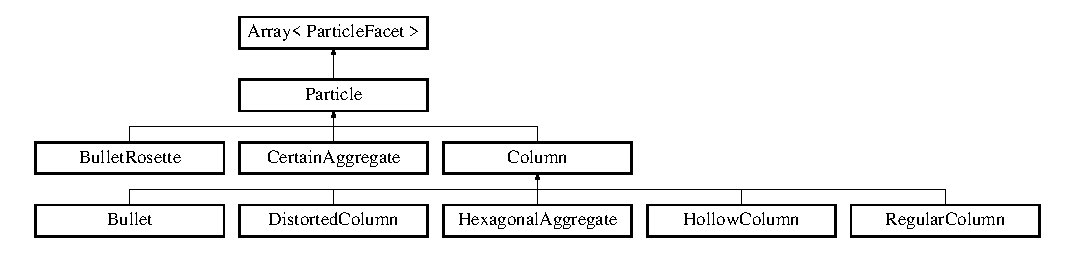
\includegraphics[height=2.947368cm]{class_particle}
\end{center}
\end{figure}
\subsection*{Public Member Functions}
\begin{DoxyCompactItemize}
\item 
\mbox{\Hypertarget{class_particle_ade07dfa403a16f3a9faad7fec89d658a}\label{class_particle_ade07dfa403a16f3a9faad7fec89d658a}} 
{\bfseries Particle} (int n\+Facets, const \mbox{\hyperlink{classcomplex}{complex}} \&refr\+Index, bool is\+Non\+Convex=false)
\item 
\mbox{\Hypertarget{class_particle_a3ea99e51c15fc69406a9d4812eff7248}\label{class_particle_a3ea99e51c15fc69406a9d4812eff7248}} 
\mbox{\hyperlink{class_facet}{Facet}} $\ast$ {\bfseries Get\+Actual\+Facet} (int i)
\item 
\mbox{\Hypertarget{class_particle_a6877eea54e7fb816809dd2be6cd5acdc}\label{class_particle_a6877eea54e7fb816809dd2be6cd5acdc}} 
void {\bfseries Set\+From\+File} (const std\+::string \&filename)
\item 
\mbox{\Hypertarget{class_particle_a55618b93d3d41f7d16af88f28dc4281b}\label{class_particle_a55618b93d3d41f7d16af88f28dc4281b}} 
void {\bfseries Rotate} (const \mbox{\hyperlink{class_angle}{Angle}} \&angle)
\item 
\mbox{\Hypertarget{class_particle_a62328fcaf288317fa6667ee9bba90de4}\label{class_particle_a62328fcaf288317fa6667ee9bba90de4}} 
void {\bfseries Move} (float dx, float dy, float dz)
\item 
\mbox{\Hypertarget{class_particle_a3e8f5b164ae0571114a98c2bafd15892}\label{class_particle_a3e8f5b164ae0571114a98c2bafd15892}} 
void {\bfseries Fix} ()
\item 
\mbox{\Hypertarget{class_particle_aecdc7104b12fab4e8485ef56546b4e1b}\label{class_particle_aecdc7104b12fab4e8485ef56546b4e1b}} 
void {\bfseries Concate} (const std\+::vector$<$ \mbox{\hyperlink{class_particle}{Particle}} $>$ \&parts)
\item 
double \mbox{\hyperlink{class_particle_ab06b62449ba3213e3f8bf580a910dd66}{Get\+Rotation\+Radius}} () const
\begin{DoxyCompactList}\small\item\em Get\+Rotation\+Radius. \end{DoxyCompactList}\item 
\mbox{\Hypertarget{class_particle_a5883ada02784b29b5cb1851f16f48066}\label{class_particle_a5883ada02784b29b5cb1851f16f48066}} 
const \mbox{\hyperlink{classcomplex}{complex}} \& {\bfseries Get\+Refractive\+Index} () const
\item 
\mbox{\Hypertarget{class_particle_a9345bfffdb91b7beb9ec48c9af29141e}\label{class_particle_a9345bfffdb91b7beb9ec48c9af29141e}} 
void {\bfseries Set\+Refractive\+Index} (const \mbox{\hyperlink{classcomplex}{complex}} \&value)
\item 
\mbox{\Hypertarget{class_particle_a29fe705a8c842ab5e31ccb94cf36fe88}\label{class_particle_a29fe705a8c842ab5e31ccb94cf36fe88}} 
const \mbox{\hyperlink{class_orientation}{Symmetry}} \& {\bfseries Get\+Symmetry} () const
\item 
\mbox{\Hypertarget{class_particle_a9e5414148dbe4bdcee8a96b9db7d1b6e}\label{class_particle_a9e5414148dbe4bdcee8a96b9db7d1b6e}} 
virtual void {\bfseries Get\+Partical\+Facet\+Id\+Range} (\mbox{\hyperlink{class_facet}{Facet}} $\ast$, int \&, int \&) const
\item 
\mbox{\Hypertarget{class_particle_a7bc2c366cbceb9fcae17d4cf8a318a73}\label{class_particle_a7bc2c366cbceb9fcae17d4cf8a318a73}} 
bool {\bfseries Is\+Non\+Convex} () const
\item 
\mbox{\Hypertarget{class_particle_aa93506becba0fc23f34c8da36c2b846b}\label{class_particle_aa93506becba0fc23f34c8da36c2b846b}} 
void {\bfseries Output} ()
\end{DoxyCompactItemize}
\subsection*{Public Attributes}
\begin{DoxyCompactItemize}
\item 
\mbox{\Hypertarget{class_particle_a57ad5c8ac7c6a4af8546210c5b4b2439}\label{class_particle_a57ad5c8ac7c6a4af8546210c5b4b2439}} 
bool {\bfseries is\+Aggregated} = false
\item 
\mbox{\Hypertarget{class_particle_a0be211b0c7c5a3148ed7bde2d15da36d}\label{class_particle_a0be211b0c7c5a3148ed7bde2d15da36d}} 
\mbox{\hyperlink{class_angle}{Angle}} {\bfseries rot\+Angle}
\end{DoxyCompactItemize}
\subsection*{Protected Member Functions}
\begin{DoxyCompactItemize}
\item 
\mbox{\Hypertarget{class_particle_a8df38703bbda2e838467a51a650624dc}\label{class_particle_a8df38703bbda2e838467a51a650624dc}} 
void {\bfseries Set\+Default\+Normals} ()
\item 
\mbox{\Hypertarget{class_particle_ab48482d12c9e0cf4eaa3a23ba9931d44}\label{class_particle_ab48482d12c9e0cf4eaa3a23ba9931d44}} 
void {\bfseries Set\+Default\+Centers} ()
\item 
\mbox{\Hypertarget{class_particle_a77d1dccca2dc8b6c2f28025256f681b8}\label{class_particle_a77d1dccca2dc8b6c2f28025256f681b8}} 
void {\bfseries Reset} ()
\item 
\mbox{\Hypertarget{class_particle_af7f8367651719a52accf283d433140bd}\label{class_particle_af7f8367651719a52accf283d433140bd}} 
void {\bfseries Set\+Symmetry} (double beta, double gamma, double alpha=0)
\item 
\mbox{\Hypertarget{class_particle_a33bf0c9eb07d48eb3e0c218554f3e20d}\label{class_particle_a33bf0c9eb07d48eb3e0c218554f3e20d}} 
virtual void {\bfseries Set\+Facet\+Params} ()
\end{DoxyCompactItemize}
\subsection*{Protected Attributes}
\begin{DoxyCompactItemize}
\item 
\mbox{\Hypertarget{class_particle_af8aaf3ce5bd6c6525543b98a23fb44a0}\label{class_particle_af8aaf3ce5bd6c6525543b98a23fb44a0}} 
\mbox{\hyperlink{class_orientation}{Symmetry}} \mbox{\hyperlink{class_particle_af8aaf3ce5bd6c6525543b98a23fb44a0}{m\+\_\+symmetry}}
\begin{DoxyCompactList}\small\item\em angle of particle symmetry \end{DoxyCompactList}\item 
\mbox{\Hypertarget{class_particle_a2285c983db1931fd823a44d104ddb578}\label{class_particle_a2285c983db1931fd823a44d104ddb578}} 
\mbox{\hyperlink{classcomplex}{complex}} \mbox{\hyperlink{class_particle_a2285c983db1931fd823a44d104ddb578}{m\+\_\+refractive\+Index}}
\begin{DoxyCompactList}\small\item\em complex value of refractive index of the particle \end{DoxyCompactList}\item 
\mbox{\Hypertarget{class_particle_a95ebda6d49685a57da79d849fca898ab}\label{class_particle_a95ebda6d49685a57da79d849fca898ab}} 
bool {\bfseries m\+\_\+is\+Non\+Convex}
\end{DoxyCompactItemize}


\subsection{Detailed Description}
The \mbox{\hyperlink{class_particle}{Particle}} class is the base class inherited by other concrete particle classes. Vertices are ordered by counterclock-\/wise direction if you see from outside. 

\subsection{Member Function Documentation}
\mbox{\Hypertarget{class_particle_ab06b62449ba3213e3f8bf580a910dd66}\label{class_particle_ab06b62449ba3213e3f8bf580a910dd66}} 
\index{Particle@{Particle}!Get\+Rotation\+Radius@{Get\+Rotation\+Radius}}
\index{Get\+Rotation\+Radius@{Get\+Rotation\+Radius}!Particle@{Particle}}
\subsubsection{\texorpdfstring{Get\+Rotation\+Radius()}{GetRotationRadius()}}
{\footnotesize\ttfamily double Particle\+::\+Get\+Rotation\+Radius (\begin{DoxyParamCaption}{ }\end{DoxyParamCaption}) const}



Get\+Rotation\+Radius. 

\begin{DoxyReturn}{Returns}
The distance from beginning of the center of coordinate system to the farthest point of particle. 
\end{DoxyReturn}


The documentation for this class was generated from the following files\+:\begin{DoxyCompactItemize}
\item 
particle/Particle.\+h\item 
particle/Particle.\+cpp\end{DoxyCompactItemize}

\hypertarget{struct_particle_facet}{}\section{Particle\+Facet Struct Reference}
\label{struct_particle_facet}\index{Particle\+Facet@{Particle\+Facet}}
\subsection*{Public Attributes}
\begin{DoxyCompactItemize}
\item 
\mbox{\Hypertarget{struct_particle_facet_a5aa003b1b0af6628c8553cb30667570f}\label{struct_particle_facet_a5aa003b1b0af6628c8553cb30667570f}} 
\mbox{\hyperlink{class_facet}{Facet}} {\bfseries origin}
\item 
\mbox{\Hypertarget{struct_particle_facet_afffaafe6140078c265ec65c984096b78}\label{struct_particle_facet_afffaafe6140078c265ec65c984096b78}} 
\mbox{\hyperlink{class_facet}{Facet}} {\bfseries actual}
\end{DoxyCompactItemize}


The documentation for this struct was generated from the following file\+:\begin{DoxyCompactItemize}
\item 
particle/Particle.\+h\end{DoxyCompactItemize}

\hypertarget{class_phis_beam}{}\section{Phis\+Beam Class Reference}
\label{class_phis_beam}\index{Phis\+Beam@{Phis\+Beam}}
Inheritance diagram for Phis\+Beam\+:\begin{figure}[H]
\begin{center}
\leavevmode
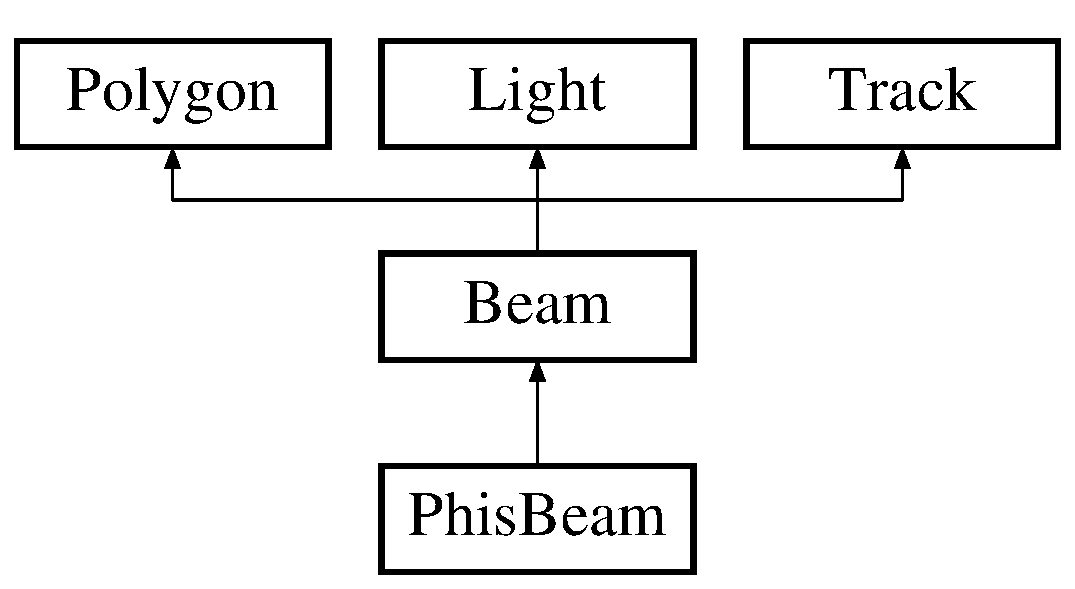
\includegraphics[height=3.000000cm]{class_phis_beam}
\end{center}
\end{figure}
\subsection*{Public Attributes}
\begin{DoxyCompactItemize}
\item 
\mbox{\Hypertarget{class_phis_beam_a31d260d43669ed31679cb41f95ca2056}\label{class_phis_beam_a31d260d43669ed31679cb41f95ca2056}} 
double \mbox{\hyperlink{class_phis_beam_a31d260d43669ed31679cb41f95ca2056}{optical\+Path}}
\begin{DoxyCompactList}\small\item\em optical path of beam \end{DoxyCompactList}\end{DoxyCompactItemize}
\subsection*{Additional Inherited Members}


The documentation for this class was generated from the following files\+:\begin{DoxyCompactItemize}
\item 
common/Phis\+Beam.\+h\item 
common/Phis\+Beam.\+cpp\end{DoxyCompactItemize}

\hypertarget{class_plane}{}\section{Plane Class Reference}
\label{class_plane}\index{Plane@{Plane}}
Inheritance diagram for Plane\+:\begin{figure}[H]
\begin{center}
\leavevmode
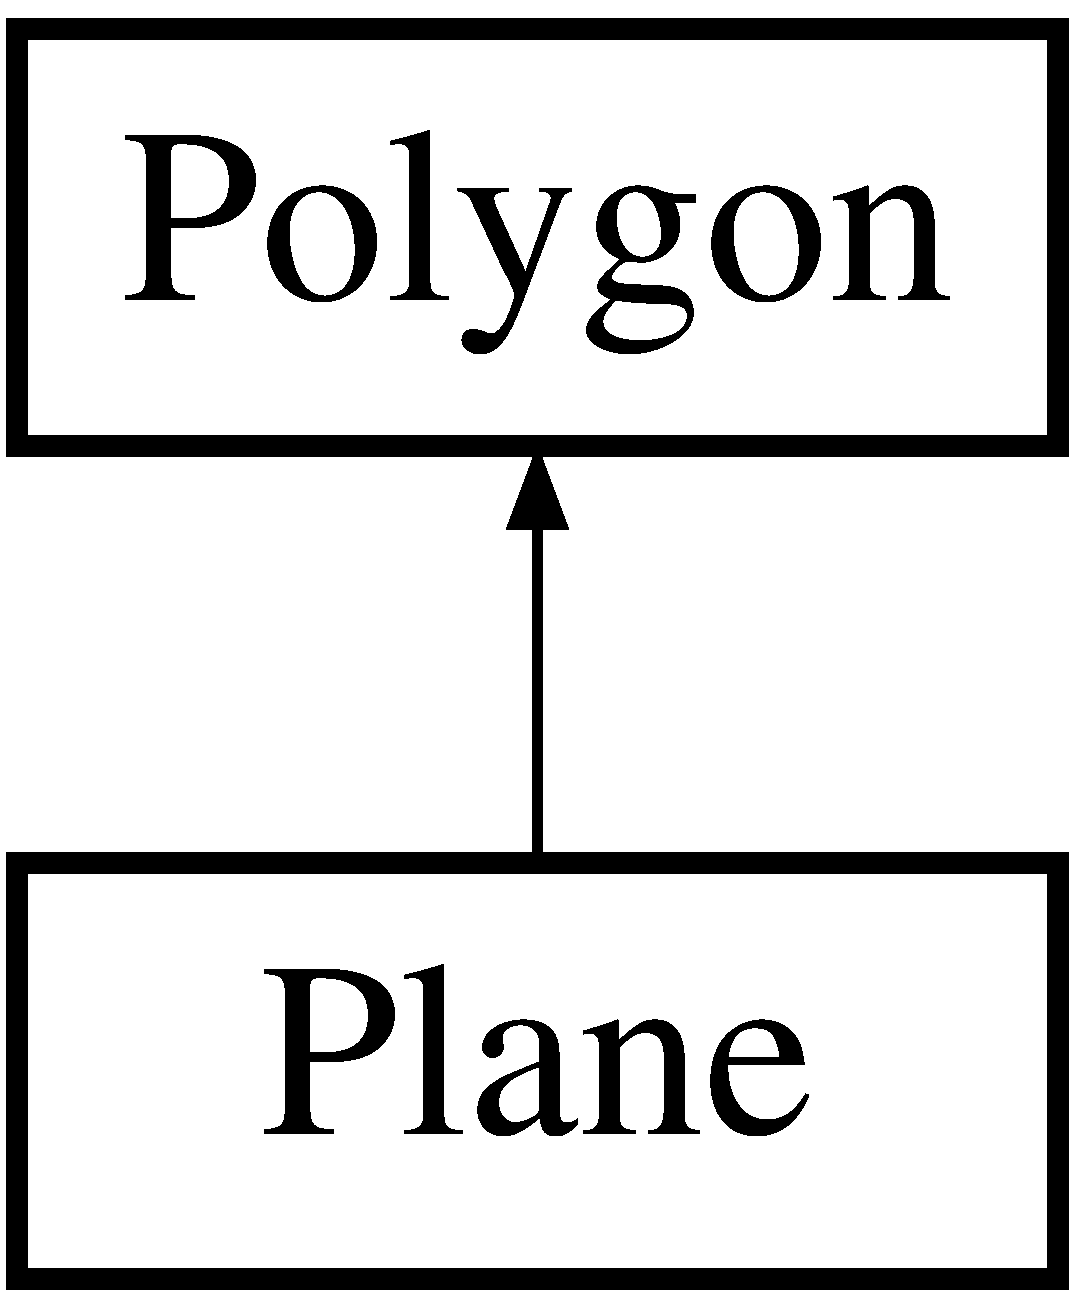
\includegraphics[height=2.000000cm]{class_plane}
\end{center}
\end{figure}
\subsection*{Public Attributes}
\begin{DoxyCompactItemize}
\item 
\mbox{\Hypertarget{class_plane_a0750005b0807c5ca32c264556d83a5d4}\label{class_plane_a0750005b0807c5ca32c264556d83a5d4}} 
\mbox{\hyperlink{struct_point3f}{Point3f}} {\bfseries normal}
\end{DoxyCompactItemize}
\subsection*{Additional Inherited Members}


The documentation for this class was generated from the following file\+:\begin{DoxyCompactItemize}
\item 
geometry/geometry\+\_\+lib.\+h\end{DoxyCompactItemize}

\hypertarget{struct_point3d}{}\section{Point3d Struct Reference}
\label{struct_point3d}\index{Point3d@{Point3d}}
\subsection*{Public Member Functions}
\begin{DoxyCompactItemize}
\item 
\mbox{\Hypertarget{struct_point3d_a1de989dba72d4b2f1b125d472c6e0238}\label{struct_point3d_a1de989dba72d4b2f1b125d472c6e0238}} 
{\bfseries Point3d} (const \mbox{\hyperlink{struct_point3f}{Point3f}} \&other)
\item 
\mbox{\Hypertarget{struct_point3d_ac6dbbcab32632b38014273d99d7a30bd}\label{struct_point3d_ac6dbbcab32632b38014273d99d7a30bd}} 
{\bfseries Point3d} (double p\+\_\+x, double p\+\_\+y, double p\+\_\+z, double p\+\_\+d=0.\+0)
\item 
\mbox{\Hypertarget{struct_point3d_a7e4a67ef61dc95cfb99f63bc32a7c036}\label{struct_point3d_a7e4a67ef61dc95cfb99f63bc32a7c036}} 
\mbox{\hyperlink{struct_point3d}{Point3d}} {\bfseries operator$\ast$} (double value) const
\item 
\mbox{\Hypertarget{struct_point3d_a25cdad9739fd3e001c513b292b79744e}\label{struct_point3d_a25cdad9739fd3e001c513b292b79744e}} 
\mbox{\hyperlink{struct_point3d}{Point3d}} {\bfseries operator+} (const \mbox{\hyperlink{struct_point3d}{Point3d}} \&other) const
\item 
\mbox{\Hypertarget{struct_point3d_af6b828bb30bf1269d8dc8cd3a555a893}\label{struct_point3d_af6b828bb30bf1269d8dc8cd3a555a893}} 
\mbox{\hyperlink{struct_point3d}{Point3d}} {\bfseries operator-\/} (const \mbox{\hyperlink{struct_point3d}{Point3d}} \&other) const
\item 
\mbox{\Hypertarget{struct_point3d_adb9c1bcd2c0ec541939cafc9b295c27f}\label{struct_point3d_adb9c1bcd2c0ec541939cafc9b295c27f}} 
\mbox{\hyperlink{struct_point3d}{Point3d}} {\bfseries operator-\/} () const
\item 
\mbox{\Hypertarget{struct_point3d_a24269a03d6217778b58dbfd6b4b9b1e7}\label{struct_point3d_a24269a03d6217778b58dbfd6b4b9b1e7}} 
\mbox{\hyperlink{struct_point3d}{Point3d}} {\bfseries operator/} (double value) const
\end{DoxyCompactItemize}
\subsection*{Static Public Member Functions}
\begin{DoxyCompactItemize}
\item 
\mbox{\Hypertarget{struct_point3d_ae22c9787e429dfe10d08729f286ddc94}\label{struct_point3d_ae22c9787e429dfe10d08729f286ddc94}} 
static double {\bfseries Dot\+Product} (const \mbox{\hyperlink{struct_point3d}{Point3d}} \&v1, const \mbox{\hyperlink{struct_point3d}{Point3d}} \&v2)
\item 
\mbox{\Hypertarget{struct_point3d_a0b4c494152c523e189e3c781f3c9736c}\label{struct_point3d_a0b4c494152c523e189e3c781f3c9736c}} 
static double {\bfseries Norm} (const \mbox{\hyperlink{struct_point3d}{Point3d}} \&p)
\item 
\mbox{\Hypertarget{struct_point3d_a09f90c67877f7bb71355762e8ba833ec}\label{struct_point3d_a09f90c67877f7bb71355762e8ba833ec}} 
static \mbox{\hyperlink{struct_point3d}{Point3d}} {\bfseries Cross\+Product} (const \mbox{\hyperlink{struct_point3d}{Point3d}} \&v1, const \mbox{\hyperlink{struct_point3d}{Point3d}} \&v2)
\item 
\mbox{\Hypertarget{struct_point3d_af9c710bb2cf8d8a6e3519ec8736c5843}\label{struct_point3d_af9c710bb2cf8d8a6e3519ec8736c5843}} 
static double {\bfseries Length} (const \mbox{\hyperlink{struct_point3d}{Point3d}} \&v)
\item 
\mbox{\Hypertarget{struct_point3d_aec6dbc891323d9449f6e3390701ec80b}\label{struct_point3d_aec6dbc891323d9449f6e3390701ec80b}} 
static \mbox{\hyperlink{struct_point3d}{Point3d}} {\bfseries Normalize} (const \mbox{\hyperlink{struct_point3d}{Point3d}} \&v)
\end{DoxyCompactItemize}
\subsection*{Public Attributes}
\begin{DoxyCompactItemize}
\item 
\mbox{\Hypertarget{struct_point3d_af07eeaead059f4d97d57921b9d04aa66}\label{struct_point3d_af07eeaead059f4d97d57921b9d04aa66}} 
double {\bfseries x}
\item 
\mbox{\Hypertarget{struct_point3d_a716403bba476bef8c1f5601542349e2c}\label{struct_point3d_a716403bba476bef8c1f5601542349e2c}} 
double {\bfseries y}
\item 
\mbox{\Hypertarget{struct_point3d_ac833626685fb5706d279ea1347b7dc17}\label{struct_point3d_ac833626685fb5706d279ea1347b7dc17}} 
double {\bfseries z}
\item 
\mbox{\Hypertarget{struct_point3d_a60413a974fd1a2955cf5a3a60c33d448}\label{struct_point3d_a60413a974fd1a2955cf5a3a60c33d448}} 
double {\bfseries d}
\end{DoxyCompactItemize}


The documentation for this struct was generated from the following file\+:\begin{DoxyCompactItemize}
\item 
geometry/Point.\+h\end{DoxyCompactItemize}

\hypertarget{struct_point3f}{}\section{Point3f Struct Reference}
\label{struct_point3f}\index{Point3f@{Point3f}}


The Point3 struct 3D coordinate point.  




{\ttfamily \#include $<$Point.\+h$>$}

\subsection*{Public Member Functions}
\begin{DoxyCompactItemize}
\item 
\mbox{\Hypertarget{struct_point3f_a2231f77480a981cfb2b0a274dd929305}\label{struct_point3f_a2231f77480a981cfb2b0a274dd929305}} 
\mbox{\hyperlink{struct_point3f_a2231f77480a981cfb2b0a274dd929305}{Point3f}} ()
\begin{DoxyCompactList}\small\item\em coordinates \end{DoxyCompactList}\item 
\mbox{\Hypertarget{struct_point3f_ab50836bbe2c4d404ef1fc82610ff327b}\label{struct_point3f_ab50836bbe2c4d404ef1fc82610ff327b}} 
{\bfseries Point3f} (float x, float y, float z)
\item 
\mbox{\Hypertarget{struct_point3f_a869413308c599aa7b86d7ce7c1f72e9f}\label{struct_point3f_a869413308c599aa7b86d7ce7c1f72e9f}} 
{\bfseries Point3f} (float x, float y, float z, float d)
\item 
\mbox{\Hypertarget{struct_point3f_a696c86a9b57a53c939f937d4378e05ab}\label{struct_point3f_a696c86a9b57a53c939f937d4378e05ab}} 
{\bfseries Point3f} (const \mbox{\hyperlink{struct_point3f}{Point3f}} \&other)
\item 
\mbox{\Hypertarget{struct_point3f_a6d35bbcaec9edaa3f018fd44556bb8dc}\label{struct_point3f_a6d35bbcaec9edaa3f018fd44556bb8dc}} 
\mbox{\hyperlink{struct_point3f}{Point3f}} \& {\bfseries operator=} (const \mbox{\hyperlink{struct_point3f}{Point3f}} \&other)
\item 
\mbox{\Hypertarget{struct_point3f_a9c08cd8213970030f6bd22607d6749ed}\label{struct_point3f_a9c08cd8213970030f6bd22607d6749ed}} 
\mbox{\hyperlink{struct_point3f}{Point3f}} {\bfseries operator$\ast$} (double value) const
\item 
\mbox{\Hypertarget{struct_point3f_af8824ee316210610951c6233eccd8018}\label{struct_point3f_af8824ee316210610951c6233eccd8018}} 
\mbox{\hyperlink{struct_point3f}{Point3f}} {\bfseries operator/} (double value) const
\item 
\mbox{\Hypertarget{struct_point3f_a14b63b81244e7b7e1b71b68a927a8770}\label{struct_point3f_a14b63b81244e7b7e1b71b68a927a8770}} 
\mbox{\hyperlink{struct_point3f}{Point3f}} {\bfseries operator-\/} (const \mbox{\hyperlink{struct_point3f}{Point3f}} \&value) const
\item 
\mbox{\Hypertarget{struct_point3f_ab51a7ed83409b4608465b0ad2c73e30e}\label{struct_point3f_ab51a7ed83409b4608465b0ad2c73e30e}} 
\mbox{\hyperlink{struct_point3f}{Point3f}} {\bfseries operator+} (const \mbox{\hyperlink{struct_point3f}{Point3f}} \&value) const
\item 
\mbox{\Hypertarget{struct_point3f_ac77dc02dc54a17dc5fa496c2013c677a}\label{struct_point3f_ac77dc02dc54a17dc5fa496c2013c677a}} 
\mbox{\hyperlink{struct_point3f}{Point3f}} {\bfseries operator+=} (double value)
\item 
\mbox{\Hypertarget{struct_point3f_a134dba0411bda961caf71a80690cf88e}\label{struct_point3f_a134dba0411bda961caf71a80690cf88e}} 
\mbox{\hyperlink{struct_point3f}{Point3f}} {\bfseries operator-\/} () const
\end{DoxyCompactItemize}
\subsection*{Static Public Member Functions}
\begin{DoxyCompactItemize}
\item 
\mbox{\Hypertarget{struct_point3f_ab6bc6585f4038a710d17f85daf8d9a9f}\label{struct_point3f_ab6bc6585f4038a710d17f85daf8d9a9f}} 
static float {\bfseries Dot\+Product} (const \mbox{\hyperlink{struct_point3f}{Point3f}} \&v1, const \mbox{\hyperlink{struct_point3f}{Point3f}} \&v2)
\item 
\mbox{\Hypertarget{struct_point3f_ab7a0686c13c8c8e8c793e86564c78071}\label{struct_point3f_ab7a0686c13c8c8e8c793e86564c78071}} 
static void {\bfseries Cross\+Product} (const \mbox{\hyperlink{struct_point3f}{Point3f}} \&v1, const \mbox{\hyperlink{struct_point3f}{Point3f}} \&v2, \mbox{\hyperlink{struct_point3f}{Point3f}} \&res)
\item 
\mbox{\Hypertarget{struct_point3f_a8200da0f3177c088c3d861529b4ee45b}\label{struct_point3f_a8200da0f3177c088c3d861529b4ee45b}} 
static \mbox{\hyperlink{struct_point3f}{Point3f}} {\bfseries Cross\+Product} (const \mbox{\hyperlink{struct_point3f}{Point3f}} \&v1, const \mbox{\hyperlink{struct_point3f}{Point3f}} \&v2)
\item 
\mbox{\Hypertarget{struct_point3f_a37fa5b749602271aa69e7e8e005fa751}\label{struct_point3f_a37fa5b749602271aa69e7e8e005fa751}} 
static double {\bfseries Norm} (const \mbox{\hyperlink{struct_point3f}{Point3f}} \&point)
\item 
\mbox{\Hypertarget{struct_point3f_ad61c0f7cc9951725b699f5e7a6051538}\label{struct_point3f_ad61c0f7cc9951725b699f5e7a6051538}} 
static void {\bfseries Normalize} (\mbox{\hyperlink{struct_point3f}{Point3f}} \&v)
\item 
\mbox{\Hypertarget{struct_point3f_aae9dbed1a41dd62e8bd420e62c3822ef}\label{struct_point3f_aae9dbed1a41dd62e8bd420e62c3822ef}} 
static double {\bfseries Length} (const \mbox{\hyperlink{struct_point3f}{Point3f}} \&v)
\end{DoxyCompactItemize}
\subsection*{Public Attributes}
\begin{DoxyCompactItemize}
\item 
\mbox{\Hypertarget{struct_point3f_a237b76269ac9e8eb01186641e65971f7}\label{struct_point3f_a237b76269ac9e8eb01186641e65971f7}} 
float {\bfseries point} \mbox{[}4\mbox{]}
\end{DoxyCompactItemize}


\subsection{Detailed Description}
The Point3 struct 3D coordinate point. 

The documentation for this struct was generated from the following files\+:\begin{DoxyCompactItemize}
\item 
geometry/Point.\+h\item 
geometry/Point.\+cpp\end{DoxyCompactItemize}

\hypertarget{class_point_contribution}{}\section{Point\+Contribution Class Reference}
\label{class_point_contribution}\index{Point\+Contribution@{Point\+Contribution}}
\subsection*{Public Member Functions}
\begin{DoxyCompactItemize}
\item 
\mbox{\Hypertarget{class_point_contribution_a8fc2f85de43e2d4f04d55878cf6a8d20}\label{class_point_contribution_a8fc2f85de43e2d4f04d55878cf6a8d20}} 
{\bfseries Point\+Contribution} (int n\+Groups, double norm\+Index)
\item 
\mbox{\Hypertarget{class_point_contribution_afb77bda8af6e19e48a69709d0b22d7a5}\label{class_point_contribution_afb77bda8af6e19e48a69709d0b22d7a5}} 
void {\bfseries Add\+To\+Mueller} (const \mbox{\hyperlink{class_matrix2x2c}{Matrix2x2c}} \&jones)
\item 
\mbox{\Hypertarget{class_point_contribution_a6939781f8a9ddb713938bcc43bf3b243}\label{class_point_contribution_a6939781f8a9ddb713938bcc43bf3b243}} 
void {\bfseries Add\+To\+Group} (const \mbox{\hyperlink{class_matrix2x2c}{Matrix2x2c}} \&jones, int group\+Id)
\item 
\mbox{\Hypertarget{class_point_contribution_a150cdb6c9d1734baeaf224edaeea5d54}\label{class_point_contribution_a150cdb6c9d1734baeaf224edaeea5d54}} 
void {\bfseries Sum\+Group\+Total} ()
\item 
\mbox{\Hypertarget{class_point_contribution_a7b1dab64cd85da8e0451d780391b9e9b}\label{class_point_contribution_a7b1dab64cd85da8e0451d780391b9e9b}} 
void {\bfseries Sum\+Total} ()
\item 
\mbox{\Hypertarget{class_point_contribution_abd8d4e97700234a92b22893da6c8155b}\label{class_point_contribution_abd8d4e97700234a92b22893da6c8155b}} 
const \mbox{\hyperlink{class_mueller_matrix}{Mueller\+Matrix}} \& {\bfseries Get\+Group\+Total} () const
\item 
\mbox{\Hypertarget{class_point_contribution_ac5e7698f3415b001c904275c249f04b8}\label{class_point_contribution_ac5e7698f3415b001c904275c249f04b8}} 
const \mbox{\hyperlink{class_mueller_matrix}{Mueller\+Matrix}} \& {\bfseries Get\+Total} () const
\item 
\mbox{\Hypertarget{class_point_contribution_a1ae18a0d167ce94f4e5d25e5e5eac6b3}\label{class_point_contribution_a1ae18a0d167ce94f4e5d25e5e5eac6b3}} 
const \mbox{\hyperlink{class_mueller_matrix}{Mueller\+Matrix}} \& {\bfseries Get\+Rest} () const
\item 
\mbox{\Hypertarget{class_point_contribution_a2c37f49735530c8c80ebb30d4be5fca3}\label{class_point_contribution_a2c37f49735530c8c80ebb30d4be5fca3}} 
const \mbox{\hyperlink{class_mueller_matrix}{Mueller\+Matrix}} \& {\bfseries Get\+Group\+Mueller} (int group\+ID)
\item 
\mbox{\Hypertarget{class_point_contribution_ae50ca6c2e611ec63043ed3fc0f109aa5}\label{class_point_contribution_ae50ca6c2e611ec63043ed3fc0f109aa5}} 
void {\bfseries Reset} ()
\end{DoxyCompactItemize}


The documentation for this class was generated from the following file\+:\begin{DoxyCompactItemize}
\item 
common/Handler.\+h\end{DoxyCompactItemize}

\hypertarget{struct_point_position}{}\section{Point\+Position Struct Reference}
\label{struct_point_position}\index{Point\+Position@{Point\+Position}}


The \mbox{\hyperlink{struct_point_position}{Point\+Position}} struct Position of point on the facet (uses in \textquotesingle{}in\+Facet\textquotesingle{} function)  




{\ttfamily \#include $<$intrinsics.\+h$>$}

\subsection*{Public Attributes}
\begin{DoxyCompactItemize}
\item 
\mbox{\Hypertarget{struct_point_position_a320fb9b9bc5e1a81131c234e879eb728}\label{struct_point_position_a320fb9b9bc5e1a81131c234e879eb728}} 
int {\bfseries position}
\item 
\mbox{\Hypertarget{struct_point_position_aba9abb7274be46364676e7152e626e69}\label{struct_point_position_aba9abb7274be46364676e7152e626e69}} 
int \mbox{\hyperlink{struct_point_position_aba9abb7274be46364676e7152e626e69}{facet\+\_\+side\+\_\+index\+\_\+1}}
\begin{DoxyCompactList}\small\item\em 1 -\/ inside, 0 -\/ on the side or vertex, -\/1 -\/ outside \end{DoxyCompactList}\item 
\mbox{\Hypertarget{struct_point_position_a566b3fefc1400a64d2015a2b7f1ea396}\label{struct_point_position_a566b3fefc1400a64d2015a2b7f1ea396}} 
int \mbox{\hyperlink{struct_point_position_a566b3fefc1400a64d2015a2b7f1ea396}{facet\+\_\+side\+\_\+index\+\_\+2}}
\begin{DoxyCompactList}\small\item\em index of side that point belongs \end{DoxyCompactList}\end{DoxyCompactItemize}


\subsection{Detailed Description}
The \mbox{\hyperlink{struct_point_position}{Point\+Position}} struct Position of point on the facet (uses in \textquotesingle{}in\+Facet\textquotesingle{} function) 

The documentation for this struct was generated from the following file\+:\begin{DoxyCompactItemize}
\item 
geometry/intrinsic/intrinsics.\+h\end{DoxyCompactItemize}

\hypertarget{class_polygon}{}\section{Polygon Class Reference}
\label{class_polygon}\index{Polygon@{Polygon}}


\mbox{\hyperlink{class_polygon}{Polygon}} consisted of 3-\/coordinate vertices.  




{\ttfamily \#include $<$Polygon.\+h$>$}



Inheritance diagram for Polygon\+:
% FIG 0


Collaboration diagram for Polygon\+:
% FIG 1
\subsection*{Public Member Functions}
\begin{DoxyCompactItemize}
\item 
\mbox{\Hypertarget{class_polygon_a30007de4ec1b150d50714a6bde4fb79d}\label{class_polygon_a30007de4ec1b150d50714a6bde4fb79d}} 
{\bfseries Polygon} (int n\+Vertices)
\item 
\mbox{\Hypertarget{class_polygon_a117451a285cc0c9d443638cd449e032b}\label{class_polygon_a117451a285cc0c9d443638cd449e032b}} 
{\bfseries Polygon} (const \mbox{\hyperlink{class_polygon}{Polygon}} \&other)
\item 
\mbox{\Hypertarget{class_polygon_ad8fc5651b8c9161a8b47b49eff09fe9c}\label{class_polygon_ad8fc5651b8c9161a8b47b49eff09fe9c}} 
{\bfseries Polygon} (\mbox{\hyperlink{class_polygon}{Polygon}} \&\&other)
\item 
\mbox{\Hypertarget{class_polygon_a073ed9d24fca614f09b23b0ed6571e36}\label{class_polygon_a073ed9d24fca614f09b23b0ed6571e36}} 
\mbox{\hyperlink{class_polygon}{Polygon}} \& {\bfseries operator=} (const \mbox{\hyperlink{class_polygon}{Polygon}} \&other)
\item 
\mbox{\Hypertarget{class_polygon_a90dd4293d3da213a7d313fd3f36b354b}\label{class_polygon_a90dd4293d3da213a7d313fd3f36b354b}} 
\mbox{\hyperlink{class_polygon}{Polygon}} \& {\bfseries operator=} (\mbox{\hyperlink{class_polygon}{Polygon}} \&\&other)
\item 
\mbox{\Hypertarget{class_polygon_a93e54fdbdb5a7de543eccbed07e0f7c8}\label{class_polygon_a93e54fdbdb5a7de543eccbed07e0f7c8}} 
double {\bfseries Area} () const
\item 
\mbox{\Hypertarget{class_polygon_a8f283e92255018b9f8331e24aaf75c57}\label{class_polygon_a8f283e92255018b9f8331e24aaf75c57}} 
\mbox{\hyperlink{struct_point3f}{Point3f}} {\bfseries Center} () const
\item 
\mbox{\Hypertarget{class_polygon_a2b1fae8937c3b44cce5022d2eee61f31}\label{class_polygon_a2b1fae8937c3b44cce5022d2eee61f31}} 
\mbox{\hyperlink{struct_point3f}{Point3f}} {\bfseries Normal} () const
\end{DoxyCompactItemize}
\subsection*{Public Attributes}
\begin{DoxyCompactItemize}
\item 
\mbox{\Hypertarget{class_polygon_a5e9924cf3d12df34b38dc75707c05254}\label{class_polygon_a5e9924cf3d12df34b38dc75707c05254}} 
\mbox{\hyperlink{struct_point3f}{Point3f}} {\bfseries arr} \mbox{[}M\+A\+X\+\_\+\+V\+E\+R\+T\+E\+X\+\_\+\+N\+UM\mbox{]}
\item 
\mbox{\Hypertarget{class_polygon_acad554243e51c93bbb13371c576006ea}\label{class_polygon_acad554243e51c93bbb13371c576006ea}} 
int {\bfseries n\+Vertices} = 0
\end{DoxyCompactItemize}
\subsection*{Friends}
\begin{DoxyCompactItemize}
\item 
\mbox{\Hypertarget{class_polygon_a3d971bd1da5beb2188d6d011bf0becdd}\label{class_polygon_a3d971bd1da5beb2188d6d011bf0becdd}} 
std\+::ostream \& {\bfseries operator$<$$<$} (std\+::ostream \&os, const \mbox{\hyperlink{class_polygon}{Polygon}} \&beam)
\end{DoxyCompactItemize}


\subsection{Detailed Description}
\mbox{\hyperlink{class_polygon}{Polygon}} consisted of 3-\/coordinate vertices. 

The documentation for this class was generated from the following files\+:\begin{DoxyCompactItemize}
\item 
geometry/Polygon.\+h\item 
geometry/Polygon.\+cpp\end{DoxyCompactItemize}

\hypertarget{class_polygon_array}{}\section{Polygon\+Array Class Reference}
\label{class_polygon_array}\index{Polygon\+Array@{Polygon\+Array}}


Collaboration diagram for Polygon\+Array\+:
% FIG 0
\subsection*{Public Member Functions}
\begin{DoxyCompactItemize}
\item 
\mbox{\Hypertarget{class_polygon_array_a333428cbdfcb87eb440f3432676f451d}\label{class_polygon_array_a333428cbdfcb87eb440f3432676f451d}} 
void {\bfseries Push} (const \mbox{\hyperlink{class_polygon}{Polygon}} \&p)
\item 
\mbox{\Hypertarget{class_polygon_array_a9267ce185f4c7f531a97ae34dc0ca3be}\label{class_polygon_array_a9267ce185f4c7f531a97ae34dc0ca3be}} 
\mbox{\hyperlink{class_polygon}{Polygon}} \& {\bfseries Pop} ()
\item 
\mbox{\Hypertarget{class_polygon_array_a70414ec458869e24c2e4445580645e3c}\label{class_polygon_array_a70414ec458869e24c2e4445580645e3c}} 
void {\bfseries Clear} ()
\end{DoxyCompactItemize}
\subsection*{Public Attributes}
\begin{DoxyCompactItemize}
\item 
\mbox{\Hypertarget{class_polygon_array_aa0414a7a6512a73053e4f159e923720b}\label{class_polygon_array_aa0414a7a6512a73053e4f159e923720b}} 
\mbox{\hyperlink{class_polygon}{Polygon}} {\bfseries arr} \mbox{[}M\+A\+X\+\_\+\+P\+O\+L\+Y\+G\+O\+N\+\_\+\+N\+UM\mbox{]}
\item 
\mbox{\Hypertarget{class_polygon_array_a59e553a53cec4121b3105ecb31e72790}\label{class_polygon_array_a59e553a53cec4121b3105ecb31e72790}} 
int {\bfseries size} = 0
\end{DoxyCompactItemize}


The documentation for this class was generated from the following file\+:\begin{DoxyCompactItemize}
\item 
geometry/Polygon.\+h\end{DoxyCompactItemize}

\hypertarget{class_clipper_lib_1_1_poly_node}{}\section{Clipper\+Lib\+:\+:Poly\+Node Class Reference}
\label{class_clipper_lib_1_1_poly_node}\index{Clipper\+Lib\+::\+Poly\+Node@{Clipper\+Lib\+::\+Poly\+Node}}
Inheritance diagram for Clipper\+Lib\+:\+:Poly\+Node\+:\begin{figure}[H]
\begin{center}
\leavevmode
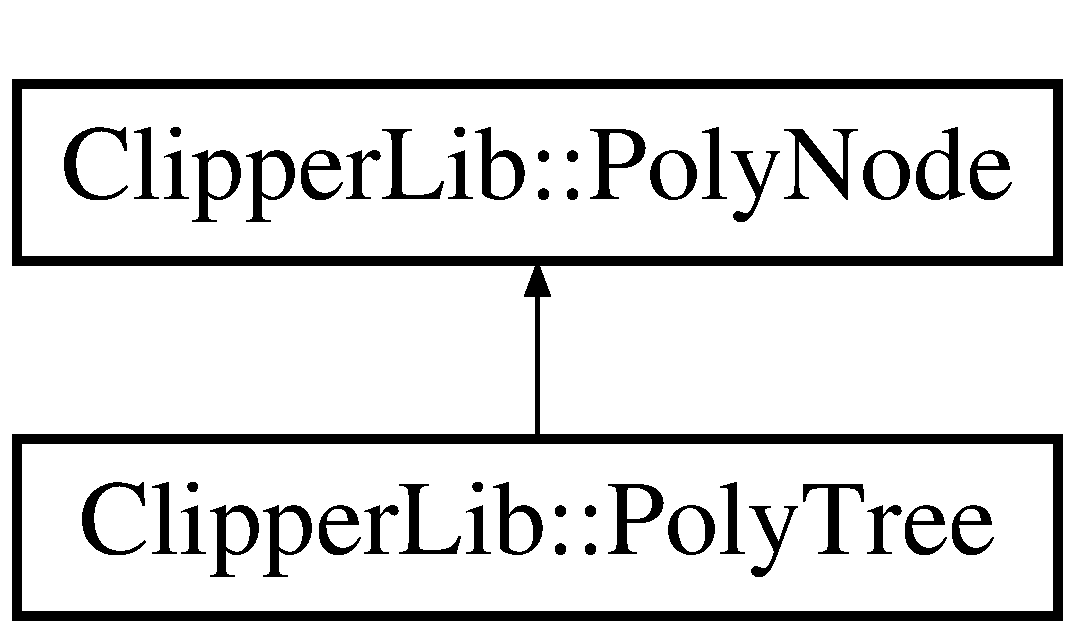
\includegraphics[height=2.000000cm]{class_clipper_lib_1_1_poly_node}
\end{center}
\end{figure}
\subsection*{Public Member Functions}
\begin{DoxyCompactItemize}
\item 
\mbox{\Hypertarget{class_clipper_lib_1_1_poly_node_adbcb861001d8bfbd609c4ba4f4a19a58}\label{class_clipper_lib_1_1_poly_node_adbcb861001d8bfbd609c4ba4f4a19a58}} 
\mbox{\hyperlink{class_clipper_lib_1_1_poly_node}{Poly\+Node}} $\ast$ {\bfseries Get\+Next} () const
\item 
\mbox{\Hypertarget{class_clipper_lib_1_1_poly_node_a0467801cae1b28ad8a4917b96e551536}\label{class_clipper_lib_1_1_poly_node_a0467801cae1b28ad8a4917b96e551536}} 
bool {\bfseries Is\+Hole} () const
\item 
\mbox{\Hypertarget{class_clipper_lib_1_1_poly_node_ac9ade640af2515976d337b65e8e84776}\label{class_clipper_lib_1_1_poly_node_ac9ade640af2515976d337b65e8e84776}} 
bool {\bfseries Is\+Open} () const
\item 
\mbox{\Hypertarget{class_clipper_lib_1_1_poly_node_a19128db6fb2aca66555231edaffa7ade}\label{class_clipper_lib_1_1_poly_node_a19128db6fb2aca66555231edaffa7ade}} 
int {\bfseries Child\+Count} () const
\end{DoxyCompactItemize}
\subsection*{Public Attributes}
\begin{DoxyCompactItemize}
\item 
\mbox{\Hypertarget{class_clipper_lib_1_1_poly_node_a1d08b8a9499ff8cb89d5d63a12f881ea}\label{class_clipper_lib_1_1_poly_node_a1d08b8a9499ff8cb89d5d63a12f881ea}} 
Path {\bfseries Contour}
\item 
\mbox{\Hypertarget{class_clipper_lib_1_1_poly_node_a7ac59aea508951a4c979bfca8913261d}\label{class_clipper_lib_1_1_poly_node_a7ac59aea508951a4c979bfca8913261d}} 
Poly\+Nodes {\bfseries Childs}
\item 
\mbox{\Hypertarget{class_clipper_lib_1_1_poly_node_a9465bc02623316de2af3ab52c6f7041e}\label{class_clipper_lib_1_1_poly_node_a9465bc02623316de2af3ab52c6f7041e}} 
\mbox{\hyperlink{class_clipper_lib_1_1_poly_node}{Poly\+Node}} $\ast$ {\bfseries Parent}
\end{DoxyCompactItemize}
\subsection*{Friends}
\begin{DoxyCompactItemize}
\item 
\mbox{\Hypertarget{class_clipper_lib_1_1_poly_node_a4d39a09ecdddeeb85930dd4554a54b3c}\label{class_clipper_lib_1_1_poly_node_a4d39a09ecdddeeb85930dd4554a54b3c}} 
class {\bfseries Clipper}
\item 
\mbox{\Hypertarget{class_clipper_lib_1_1_poly_node_adadfb8ac9a17a5c8fb7b4f012075b975}\label{class_clipper_lib_1_1_poly_node_adadfb8ac9a17a5c8fb7b4f012075b975}} 
class {\bfseries Clipper\+Offset}
\end{DoxyCompactItemize}


The documentation for this class was generated from the following files\+:\begin{DoxyCompactItemize}
\item 
geometry/clipper/clipper.\+hpp\item 
geometry/clipper/clipper.\+cpp\end{DoxyCompactItemize}

\hypertarget{class_clipper_lib_1_1_poly_tree}{}\section{Clipper\+Lib\+:\+:Poly\+Tree Class Reference}
\label{class_clipper_lib_1_1_poly_tree}\index{Clipper\+Lib\+::\+Poly\+Tree@{Clipper\+Lib\+::\+Poly\+Tree}}
Inheritance diagram for Clipper\+Lib\+:\+:Poly\+Tree\+:\begin{figure}[H]
\begin{center}
\leavevmode
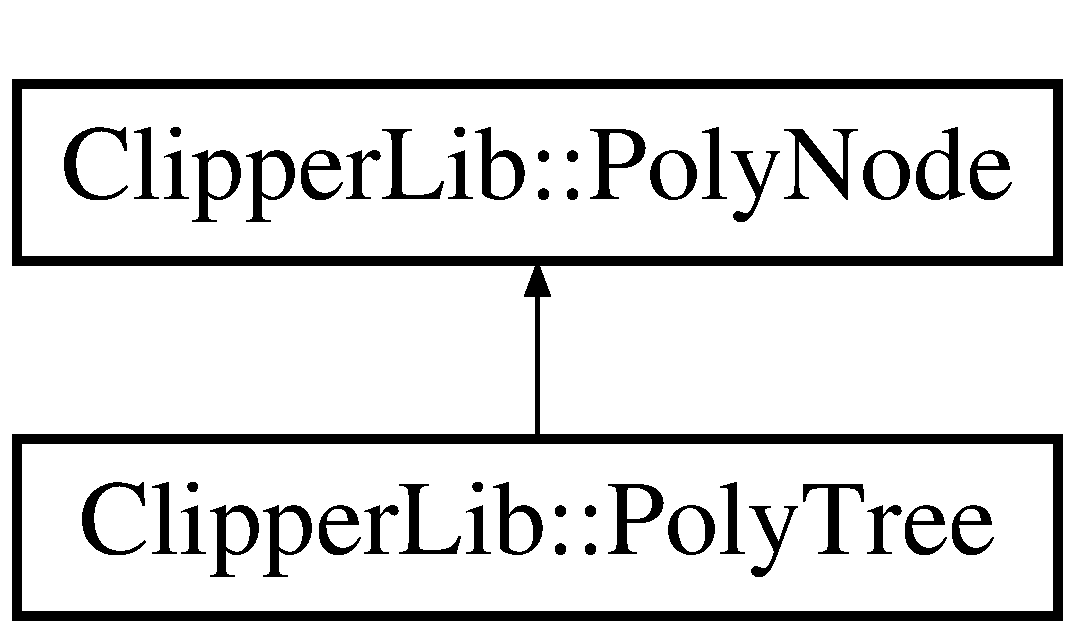
\includegraphics[height=2.000000cm]{class_clipper_lib_1_1_poly_tree}
\end{center}
\end{figure}
\subsection*{Public Member Functions}
\begin{DoxyCompactItemize}
\item 
\mbox{\Hypertarget{class_clipper_lib_1_1_poly_tree_a8b88b8d6225281ee7d536902b0d04e9e}\label{class_clipper_lib_1_1_poly_tree_a8b88b8d6225281ee7d536902b0d04e9e}} 
\mbox{\hyperlink{class_clipper_lib_1_1_poly_node}{Poly\+Node}} $\ast$ {\bfseries Get\+First} () const
\item 
\mbox{\Hypertarget{class_clipper_lib_1_1_poly_tree_a8620ea631d478b3c43274ac084902ec4}\label{class_clipper_lib_1_1_poly_tree_a8620ea631d478b3c43274ac084902ec4}} 
void {\bfseries Clear} ()
\item 
\mbox{\Hypertarget{class_clipper_lib_1_1_poly_tree_ad0d3c974bab5a30cc8c916da9fe14388}\label{class_clipper_lib_1_1_poly_tree_ad0d3c974bab5a30cc8c916da9fe14388}} 
int {\bfseries Total} () const
\end{DoxyCompactItemize}
\subsection*{Friends}
\begin{DoxyCompactItemize}
\item 
\mbox{\Hypertarget{class_clipper_lib_1_1_poly_tree_a4d39a09ecdddeeb85930dd4554a54b3c}\label{class_clipper_lib_1_1_poly_tree_a4d39a09ecdddeeb85930dd4554a54b3c}} 
class {\bfseries Clipper}
\end{DoxyCompactItemize}
\subsection*{Additional Inherited Members}


The documentation for this class was generated from the following files\+:\begin{DoxyCompactItemize}
\item 
geometry/clipper/clipper.\+hpp\item 
geometry/clipper/clipper.\+cpp\end{DoxyCompactItemize}

\hypertarget{class_regular_column}{}\section{Regular\+Column Class Reference}
\label{class_regular_column}\index{Regular\+Column@{Regular\+Column}}


Inheritance diagram for Regular\+Column\+:
% FIG 0


Collaboration diagram for Regular\+Column\+:
% FIG 1
\subsection*{Public Member Functions}
\begin{DoxyCompactItemize}
\item 
\mbox{\Hypertarget{class_regular_column_a812a5c38e59e8c467db27253cc993eff}\label{class_regular_column_a812a5c38e59e8c467db27253cc993eff}} 
{\bfseries Regular\+Column} (const \mbox{\hyperlink{classcomplex}{complex}} \&refr\+Index, const \mbox{\hyperlink{struct_size}{Size}} \&size)
\end{DoxyCompactItemize}
\subsection*{Additional Inherited Members}


The documentation for this class was generated from the following files\+:\begin{DoxyCompactItemize}
\item 
particle/Regular\+Column.\+h\item 
particle/Regular\+Column.\+cpp\end{DoxyCompactItemize}

\hypertarget{class_regular_incidence}{}\section{Regular\+Incidence Class Reference}
\label{class_regular_incidence}\index{Regular\+Incidence@{Regular\+Incidence}}


Inheritance diagram for Regular\+Incidence\+:
% FIG 0


Collaboration diagram for Regular\+Incidence\+:
% FIG 1
\subsection*{Public Member Functions}
\begin{DoxyCompactItemize}
\item 
\mbox{\Hypertarget{class_regular_incidence_a8ecdb90673e76607d064435681107169}\label{class_regular_incidence_a8ecdb90673e76607d064435681107169}} 
virtual void {\bfseries Compute\+Directions} (\mbox{\hyperlink{class_beam}{Beam}} \&beam, \mbox{\hyperlink{class_splitting}{Splitting}} \&splitter) const override
\item 
\mbox{\Hypertarget{class_regular_incidence_aef24ed873633d428aa0d9bd0f898fe13}\label{class_regular_incidence_aef24ed873633d428aa0d9bd0f898fe13}} 
virtual void {\bfseries Compute\+Jones\+Matrices} (\mbox{\hyperlink{class_beam}{Beam}} \&beam, \mbox{\hyperlink{class_splitting}{Splitting}} \&splitter) const override
\end{DoxyCompactItemize}


The documentation for this class was generated from the following files\+:\begin{DoxyCompactItemize}
\item 
incidence/Regular\+Incidence.\+h\item 
incidence/Regular\+Incidence.\+cpp\end{DoxyCompactItemize}

\hypertarget{class_scattering}{}\section{Scattering Class Reference}
\label{class_scattering}\index{Scattering@{Scattering}}


Produce a set of beams from a light that incident on a \mbox{\hyperlink{class_particle}{Particle}}.  




{\ttfamily \#include $<$Scattering.\+h$>$}



Inheritance diagram for Scattering\+:
% FIG 0


Collaboration diagram for Scattering\+:
% FIG 1
\subsection*{Public Member Functions}
\begin{DoxyCompactItemize}
\item 
\mbox{\Hypertarget{class_scattering_aa7c9e78a57111fd2cbf858f1c453283f}\label{class_scattering_aa7c9e78a57111fd2cbf858f1c453283f}} 
{\bfseries Scattering} (\mbox{\hyperlink{class_particle}{Particle}} $\ast$particle, const \mbox{\hyperlink{class_light}{Light}} \&incident\+Light, int max\+Act\+No)
\item 
void \mbox{\hyperlink{class_scattering_ab428bc4f6c26d02bcf7044e653cdf523}{Scatter\+Light}} (std\+::vector$<$ \mbox{\hyperlink{class_beam}{Beam}} $>$ \&scaterred\+Beams)
\begin{DoxyCompactList}\small\item\em Tranform incident light into beams after throwing the \mbox{\hyperlink{class_particle}{Particle}}. \end{DoxyCompactList}\item 
\mbox{\Hypertarget{class_scattering_afb9b9c16fc45f08a0a2b1bdaa14fdb9a}\label{class_scattering_afb9b9c16fc45f08a0a2b1bdaa14fdb9a}} 
double {\bfseries Get\+Incident\+Energy} () const
\item 
\mbox{\Hypertarget{class_scattering_ac628a914ca4f93914df8cc3e64b03636}\label{class_scattering_ac628a914ca4f93914df8cc3e64b03636}} 
\mbox{\hyperlink{struct_optical_path}{Optical\+Path}} {\bfseries Compute\+Optical\+Path} (const \mbox{\hyperlink{class_beam}{Beam}} \&beam, const \mbox{\hyperlink{struct_point3f}{Point3f}} \&start\+Point, std\+::vector$<$ int $>$ track)
\end{DoxyCompactItemize}
\subsection*{Protected Member Functions}
\begin{DoxyCompactItemize}
\item 
\mbox{\Hypertarget{class_scattering_a4b891bd6dcd276e42f2697cf6cd35f2b}\label{class_scattering_a4b891bd6dcd276e42f2697cf6cd35f2b}} 
virtual void {\bfseries Split\+Origin\+Beam} (std\+::vector$<$ \mbox{\hyperlink{class_beam}{Beam}} $>$ \&scattered\+Beams)=0
\item 
virtual void \mbox{\hyperlink{class_scattering_a6fa2a9f952577d5310d8a8e617f2c8f8}{Release\+Beam}} (\mbox{\hyperlink{class_beam}{Beam}} \&beam)
\begin{DoxyCompactList}\small\item\em Final handling of beam and throwing it out of the \mbox{\hyperlink{class_particle}{Particle}}. \end{DoxyCompactList}\item 
virtual bool \mbox{\hyperlink{class_scattering_abe93cd1898e52b1601c96735020454fe}{Is\+Terminal\+Act}} (const \mbox{\hyperlink{class_beam}{Beam}} \&beam)
\begin{DoxyCompactList}\small\item\em Checks if beam has been to release out of \mbox{\hyperlink{class_particle}{Particle}}. \end{DoxyCompactList}\item 
\mbox{\Hypertarget{class_scattering_a9223cd083c3567785d7aa6cf1c48264f}\label{class_scattering_a9223cd083c3567785d7aa6cf1c48264f}} 
virtual bool {\bfseries is\+Terminal\+Facet} (int index, \mbox{\hyperlink{class_array}{Array}}$<$ \mbox{\hyperlink{class_facet}{Facet}} $\ast$$>$ \&facets)
\item 
\mbox{\Hypertarget{class_scattering_a3e69b875202c73dfff77d7c4e7f9cc2a}\label{class_scattering_a3e69b875202c73dfff77d7c4e7f9cc2a}} 
virtual void {\bfseries Select\+Visible\+Facets} (const \mbox{\hyperlink{class_beam}{Beam}} \&beam, \mbox{\hyperlink{class_array}{Array}}$<$ \mbox{\hyperlink{class_facet}{Facet}} $\ast$$>$ \&facets)=0
\item 
\mbox{\Hypertarget{class_scattering_a8c8b0bcf34e7b810fdc589130adec1d6}\label{class_scattering_a8c8b0bcf34e7b810fdc589130adec1d6}} 
virtual void {\bfseries Push\+Beams\+To\+Buffer} (\mbox{\hyperlink{class_beam}{Beam}} \&parent\+Beam, \mbox{\hyperlink{class_facet}{Facet}} $\ast$facet, bool has\+Out\+Beam)
\item 
\mbox{\Hypertarget{class_scattering_aee7284ceaca09534124e9a204897745c}\label{class_scattering_aee7284ceaca09534124e9a204897745c}} 
void {\bfseries Split\+Secondary\+Beams} (std\+::vector$<$ \mbox{\hyperlink{class_beam}{Beam}} $>$ \&scattered\+Beams)
\item 
\mbox{\Hypertarget{class_scattering_a122537e571cab317861d6dd37a4ce5bf}\label{class_scattering_a122537e571cab317861d6dd37a4ce5bf}} 
void {\bfseries Split\+Beam\+By\+Visible\+Facets} (\mbox{\hyperlink{class_beam}{Beam}} \&beam)
\item 
\mbox{\Hypertarget{class_scattering_ad6ca3dd6451a0d0976ba593cdf68c0f4}\label{class_scattering_ad6ca3dd6451a0d0976ba593cdf68c0f4}} 
void {\bfseries Find\+Visible\+Facets} (const \mbox{\hyperlink{class_beam}{Beam}} \&beam, \mbox{\hyperlink{class_facet_checker}{Facet\+Checker}} \&checker, int begin, int end, \mbox{\hyperlink{class_array}{Array}}$<$ \mbox{\hyperlink{class_facet}{Facet}} $\ast$$>$ \&facets)
\item 
\mbox{\Hypertarget{class_scattering_ac80e5b8c758fcf6c04d6af47b7c87a56}\label{class_scattering_ac80e5b8c758fcf6c04d6af47b7c87a56}} 
bool {\bfseries Compute\+Optical\+Beam\+Params} (\mbox{\hyperlink{class_facet}{Facet}} $\ast$facet, \mbox{\hyperlink{class_beam}{Beam}} beam)
\item 
void \mbox{\hyperlink{class_scattering_abdf7a6563ec37996654fa59ab99bab3f}{Set\+Polygon\+By\+Facet}} (\mbox{\hyperlink{class_facet}{Facet}} $\ast$facet, \mbox{\hyperlink{class_polygon}{Polygon}} \&polygon) const
\item 
\mbox{\Hypertarget{class_scattering_acccb70145215368218d90cf4bd93b63b}\label{class_scattering_acccb70145215368218d90cf4bd93b63b}} 
\mbox{\hyperlink{struct_point3f}{Point3f}} {\bfseries Compute\+Beam\+Direction} (const \mbox{\hyperlink{struct_point3f}{Vector3f}} \&old\+Dir, const \mbox{\hyperlink{struct_point3f}{Vector3f}} \&normal, bool is\+In1, bool is\+In2)
\item 
\mbox{\Hypertarget{class_scattering_ac1b11b96eaa2a09c4595f4d0f65c5dbe}\label{class_scattering_ac1b11b96eaa2a09c4595f4d0f65c5dbe}} 
void {\bfseries Compute\+Facet\+Energy} (const \mbox{\hyperlink{struct_point3f}{Vector3f}} \&facet\+Normal, const \mbox{\hyperlink{class_polygon}{Polygon}} \&lighted\+Polygon)
\item 
\mbox{\Hypertarget{class_scattering_a005cde1e87267a9e4c009958d6ee311a}\label{class_scattering_a005cde1e87267a9e4c009958d6ee311a}} 
void {\bfseries Push\+Beam\+To\+Tree} (\mbox{\hyperlink{class_beam}{Beam}} \&beam)
\item 
\mbox{\Hypertarget{class_scattering_aacb21df97d1762f127b78da0cb2471a2}\label{class_scattering_aacb21df97d1762f127b78da0cb2471a2}} 
void {\bfseries Create\+Origin\+Beam} (const \mbox{\hyperlink{struct_point3f}{Vector3f}} \&dir, const \mbox{\hyperlink{struct_point3f}{Vector3f}} \&basis)
\end{DoxyCompactItemize}
\subsection*{Protected Attributes}
\begin{DoxyCompactItemize}
\item 
\mbox{\Hypertarget{class_scattering_aabab038d88c737bb87dd777175b9d541}\label{class_scattering_aabab038d88c737bb87dd777175b9d541}} 
\mbox{\hyperlink{class_particle}{Particle}} $\ast$ \mbox{\hyperlink{class_scattering_aabab038d88c737bb87dd777175b9d541}{m\+\_\+particle}}
\begin{DoxyCompactList}\small\item\em The crystal for a light scattering. \end{DoxyCompactList}\item 
\mbox{\Hypertarget{class_scattering_a208510c2d17cdcf221d372ef09441c61}\label{class_scattering_a208510c2d17cdcf221d372ef09441c61}} 
int \mbox{\hyperlink{class_scattering_a208510c2d17cdcf221d372ef09441c61}{m\+\_\+max\+Act\+No}}
\begin{DoxyCompactList}\small\item\em Maximal number of reflection/refraction acts. \end{DoxyCompactList}\item 
\mbox{\Hypertarget{class_scattering_aa4535b7a8928911c533fb4f6f026e75d}\label{class_scattering_aa4535b7a8928911c533fb4f6f026e75d}} 
\mbox{\hyperlink{class_splitting}{Splitting}} {\bfseries m\+\_\+splitting}
\item 
\mbox{\Hypertarget{class_scattering_a807c34a5a7fdf1cf3bb9939b06d1d063}\label{class_scattering_a807c34a5a7fdf1cf3bb9939b06d1d063}} 
\mbox{\hyperlink{class_light_facet_checker}{Light\+Facet\+Checker}} {\bfseries m\+\_\+light\+Checker}
\item 
\mbox{\Hypertarget{class_scattering_ad211279d6de0e1e825a44c28927b6acc}\label{class_scattering_ad211279d6de0e1e825a44c28927b6acc}} 
\mbox{\hyperlink{class_beam_facet_checker}{Beam\+Facet\+Checker}} {\bfseries m\+\_\+beam\+Checker}
\item 
\mbox{\hyperlink{class_beam}{Beam}} \mbox{\hyperlink{class_scattering_a82f0c3297cbde80cd091a503428f2dc5}{m\+\_\+origin\+Beam}}
\item 
\mbox{\Hypertarget{class_scattering_adac874d581f21d2e90eb8004e50f3086}\label{class_scattering_adac874d581f21d2e90eb8004e50f3086}} 
\mbox{\hyperlink{class_beam}{Beam}} \mbox{\hyperlink{class_scattering_adac874d581f21d2e90eb8004e50f3086}{m\+\_\+propagating\+Beams}} \mbox{[}M\+A\+X\+\_\+\+B\+E\+A\+M\+\_\+\+N\+UM\mbox{]}
\begin{DoxyCompactList}\small\item\em Beams that are waiting for the next r/r act. \end{DoxyCompactList}\item 
\mbox{\Hypertarget{class_scattering_adb62197742a6ee9e1b9c3e988a4a89ee}\label{class_scattering_adb62197742a6ee9e1b9c3e988a4a89ee}} 
int {\bfseries m\+\_\+tree\+Size}
\item 
\mbox{\Hypertarget{class_scattering_ac35fa41714a7784304eead96b8186532}\label{class_scattering_ac35fa41714a7784304eead96b8186532}} 
std\+::vector$<$ \mbox{\hyperlink{class_beam}{Beam}} $>$ $\ast$ {\bfseries m\+\_\+scattered\+Beams}
\item 
\mbox{\Hypertarget{class_scattering_a7a80cb232adf041261fe02811c5cdfd5}\label{class_scattering_a7a80cb232adf041261fe02811c5cdfd5}} 
\mbox{\hyperlink{class_array}{Array}}$<$ \mbox{\hyperlink{class_facet}{Facet}} $\ast$ $>$ {\bfseries m\+\_\+visible\+Facets}
\item 
\mbox{\Hypertarget{class_scattering_a698c33191f5e87477b37b27e36bca0a2}\label{class_scattering_a698c33191f5e87477b37b27e36bca0a2}} 
double {\bfseries m\+\_\+incident\+Energy}
\item 
\mbox{\Hypertarget{class_scattering_a172f9184deb0e131762f21cd33a02788}\label{class_scattering_a172f9184deb0e131762f21cd33a02788}} 
const double {\bfseries E\+P\+S\+\_\+\+B\+E\+A\+M\+\_\+\+E\+N\+E\+R\+GY} = 2e-\/12
\end{DoxyCompactItemize}


\subsection{Detailed Description}
Produce a set of beams from a light that incident on a \mbox{\hyperlink{class_particle}{Particle}}. 

\subsection{Member Function Documentation}
\mbox{\Hypertarget{class_scattering_abe93cd1898e52b1601c96735020454fe}\label{class_scattering_abe93cd1898e52b1601c96735020454fe}} 
\index{Scattering@{Scattering}!Is\+Terminal\+Act@{Is\+Terminal\+Act}}
\index{Is\+Terminal\+Act@{Is\+Terminal\+Act}!Scattering@{Scattering}}
\subsubsection{\texorpdfstring{Is\+Terminal\+Act()}{IsTerminalAct()}}
{\footnotesize\ttfamily bool Scattering\+::\+Is\+Terminal\+Act (\begin{DoxyParamCaption}\item[{const \mbox{\hyperlink{class_beam}{Beam}} \&}]{beam }\end{DoxyParamCaption})\hspace{0.3cm}{\ttfamily [protected]}, {\ttfamily [virtual]}}



Checks if beam has been to release out of \mbox{\hyperlink{class_particle}{Particle}}. 


\begin{DoxyParams}{Parameters}
{\em beam} & checked beam \\
\hline
\end{DoxyParams}
\begin{DoxyReturn}{Returns}
true if beam has been to release, false otherwise 
\end{DoxyReturn}


Reimplemented in \mbox{\hyperlink{class_scattering_non_convex_aeda4103d997bc16e155fcc8281a51b05}{Scattering\+Non\+Convex}}.

Here is the caller graph for this function\+:
% FIG 2
\mbox{\Hypertarget{class_scattering_a6fa2a9f952577d5310d8a8e617f2c8f8}\label{class_scattering_a6fa2a9f952577d5310d8a8e617f2c8f8}} 
\index{Scattering@{Scattering}!Release\+Beam@{Release\+Beam}}
\index{Release\+Beam@{Release\+Beam}!Scattering@{Scattering}}
\subsubsection{\texorpdfstring{Release\+Beam()}{ReleaseBeam()}}
{\footnotesize\ttfamily void Scattering\+::\+Release\+Beam (\begin{DoxyParamCaption}\item[{\mbox{\hyperlink{class_beam}{Beam}} \&}]{beam }\end{DoxyParamCaption})\hspace{0.3cm}{\ttfamily [protected]}, {\ttfamily [virtual]}}



Final handling of beam and throwing it out of the \mbox{\hyperlink{class_particle}{Particle}}. 


\begin{DoxyParams}{Parameters}
{\em beam} & throwed beam \\
\hline
{\em scattered\+Beams} & output buffer \\
\hline
\end{DoxyParams}


Reimplemented in \mbox{\hyperlink{class_scattering_non_convex_a574f2c4d503c6751f374e37e632f584a}{Scattering\+Non\+Convex}}.

Here is the caller graph for this function\+:
% FIG 3
\mbox{\Hypertarget{class_scattering_ab428bc4f6c26d02bcf7044e653cdf523}\label{class_scattering_ab428bc4f6c26d02bcf7044e653cdf523}} 
\index{Scattering@{Scattering}!Scatter\+Light@{Scatter\+Light}}
\index{Scatter\+Light@{Scatter\+Light}!Scattering@{Scattering}}
\subsubsection{\texorpdfstring{Scatter\+Light()}{ScatterLight()}}
{\footnotesize\ttfamily void Scattering\+::\+Scatter\+Light (\begin{DoxyParamCaption}\item[{std\+::vector$<$ \mbox{\hyperlink{class_beam}{Beam}} $>$ \&}]{scaterred\+Beams }\end{DoxyParamCaption})}



Tranform incident light into beams after throwing the \mbox{\hyperlink{class_particle}{Particle}}. 


\begin{DoxyParams}{Parameters}
{\em scaterred\+Beams} & result beams \\
\hline
\end{DoxyParams}
\mbox{\Hypertarget{class_scattering_abdf7a6563ec37996654fa59ab99bab3f}\label{class_scattering_abdf7a6563ec37996654fa59ab99bab3f}} 
\index{Scattering@{Scattering}!Set\+Polygon\+By\+Facet@{Set\+Polygon\+By\+Facet}}
\index{Set\+Polygon\+By\+Facet@{Set\+Polygon\+By\+Facet}!Scattering@{Scattering}}
\subsubsection{\texorpdfstring{Set\+Polygon\+By\+Facet()}{SetPolygonByFacet()}}
{\footnotesize\ttfamily void Scattering\+::\+Set\+Polygon\+By\+Facet (\begin{DoxyParamCaption}\item[{\mbox{\hyperlink{class_facet}{Facet}} $\ast$}]{facet,  }\item[{\mbox{\hyperlink{class_polygon}{Polygon}} \&}]{polygon }\end{DoxyParamCaption}) const\hspace{0.3cm}{\ttfamily [protected]}}

N\+O\+TE\+: Result beams are ordered in inverse direction 

\subsection{Member Data Documentation}
\mbox{\Hypertarget{class_scattering_a82f0c3297cbde80cd091a503428f2dc5}\label{class_scattering_a82f0c3297cbde80cd091a503428f2dc5}} 
\index{Scattering@{Scattering}!m\+\_\+origin\+Beam@{m\+\_\+origin\+Beam}}
\index{m\+\_\+origin\+Beam@{m\+\_\+origin\+Beam}!Scattering@{Scattering}}
\subsubsection{\texorpdfstring{m\+\_\+origin\+Beam}{m\_originBeam}}
{\footnotesize\ttfamily \mbox{\hyperlink{class_beam}{Beam}} Scattering\+::m\+\_\+origin\+Beam\hspace{0.3cm}{\ttfamily [protected]}}

The first beam that incident on a \mbox{\hyperlink{class_particle}{Particle}}. It has no boundaries (i.\+e. \mbox{\hyperlink{class_polygon}{Polygon}} is empty) 

The documentation for this class was generated from the following files\+:\begin{DoxyCompactItemize}
\item 
scattering/Scattering.\+h\item 
scattering/Scattering.\+cpp\end{DoxyCompactItemize}

\hypertarget{class_scattering_convex}{}\section{Scattering\+Convex Class Reference}
\label{class_scattering_convex}\index{Scattering\+Convex@{Scattering\+Convex}}
Inheritance diagram for Scattering\+Convex\+:\begin{figure}[H]
\begin{center}
\leavevmode
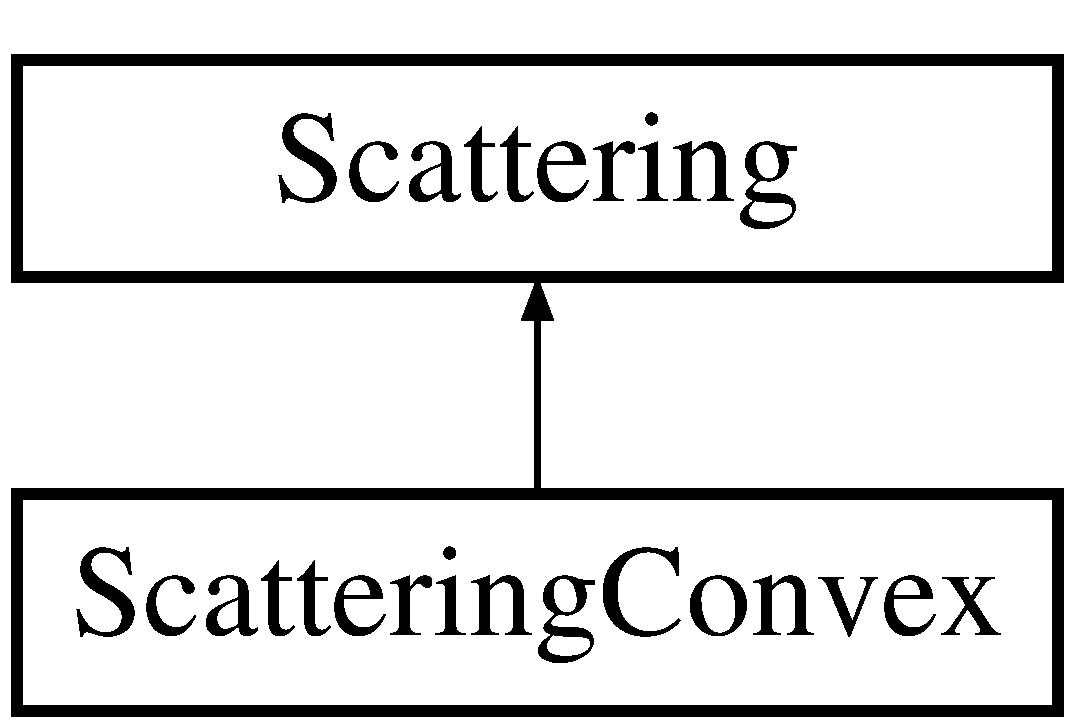
\includegraphics[height=2.000000cm]{class_scattering_convex}
\end{center}
\end{figure}
\subsection*{Public Member Functions}
\begin{DoxyCompactItemize}
\item 
\mbox{\Hypertarget{class_scattering_convex_a9adedd65ccc3aff302db10a7609d6b18}\label{class_scattering_convex_a9adedd65ccc3aff302db10a7609d6b18}} 
{\bfseries Scattering\+Convex} (\mbox{\hyperlink{class_particle}{Particle}} $\ast$particle, \mbox{\hyperlink{class_light}{Light}} $\ast$incident\+Light, bool is\+Optical\+Path, int n\+Acts)
\end{DoxyCompactItemize}
\subsection*{Protected Member Functions}
\begin{DoxyCompactItemize}
\item 
\mbox{\Hypertarget{class_scattering_convex_a9f7ef5a3606a49f8be327cb966d217bb}\label{class_scattering_convex_a9f7ef5a3606a49f8be327cb966d217bb}} 
void {\bfseries Scatter\+Beams} (std\+::vector$<$ \mbox{\hyperlink{class_beam}{Beam}} $>$ \&scattered\+Beams) override
\item 
void \mbox{\hyperlink{class_scattering_convex_acb8aa7121ffd9dfb7bf1d51a0d68e93a}{Split\+Light\+To\+Beams}} (std\+::vector$<$ \mbox{\hyperlink{class_beam}{Beam}} $>$ \&scattered\+Beams) override
\item 
\mbox{\Hypertarget{class_scattering_convex_a4a2db66ffa5fa5c9190bd1f509ff02cc}\label{class_scattering_convex_a4a2db66ffa5fa5c9190bd1f509ff02cc}} 
void {\bfseries Split\+Beams\+By\+Facet} (\mbox{\hyperlink{class_beam}{Beam}} \&beam, \mbox{\hyperlink{class_facet}{Facet}} $\ast$facet, std\+::vector$<$ \mbox{\hyperlink{class_beam}{Beam}} $>$ \&scattered\+Beams)
\end{DoxyCompactItemize}
\subsection*{Additional Inherited Members}


\subsection{Member Function Documentation}
\mbox{\Hypertarget{class_scattering_convex_acb8aa7121ffd9dfb7bf1d51a0d68e93a}\label{class_scattering_convex_acb8aa7121ffd9dfb7bf1d51a0d68e93a}} 
\index{Scattering\+Convex@{Scattering\+Convex}!Split\+Light\+To\+Beams@{Split\+Light\+To\+Beams}}
\index{Split\+Light\+To\+Beams@{Split\+Light\+To\+Beams}!Scattering\+Convex@{Scattering\+Convex}}
\subsubsection{\texorpdfstring{Split\+Light\+To\+Beams()}{SplitLightToBeams()}}
{\footnotesize\ttfamily void Scattering\+Convex\+::\+Split\+Light\+To\+Beams (\begin{DoxyParamCaption}\item[{std\+::vector$<$ \mbox{\hyperlink{class_beam}{Beam}} $>$ \&}]{scattered\+Beams }\end{DoxyParamCaption})\hspace{0.3cm}{\ttfamily [override]}, {\ttfamily [protected]}, {\ttfamily [virtual]}}

beam is not incident to this facet 

Implements \mbox{\hyperlink{class_scattering}{Scattering}}.



The documentation for this class was generated from the following files\+:\begin{DoxyCompactItemize}
\item 
scattering/Scattering\+Convex.\+h\item 
scattering/Scattering\+Convex.\+cpp\end{DoxyCompactItemize}

\hypertarget{class_scattering_files}{}\section{Scattering\+Files Class Reference}
\label{class_scattering_files}\index{Scattering\+Files@{Scattering\+Files}}
\subsection*{Public Member Functions}
\begin{DoxyCompactItemize}
\item 
\mbox{\Hypertarget{class_scattering_files_a00914cfb3a0c6f24b02c3614defb1f2c}\label{class_scattering_files_a00914cfb3a0c6f24b02c3614defb1f2c}} 
{\bfseries Scattering\+Files} (const std\+::string \&dir, const std\+::string \&folder, const std\+::string \&table\+Head=\char`\"{}\char`\"{})
\item 
\mbox{\Hypertarget{class_scattering_files_aabb3077522bad53f58e84445019f970f}\label{class_scattering_files_aabb3077522bad53f58e84445019f970f}} 
void {\bfseries Create\+Main\+File} (const std\+::string \&subdir, const std\+::string \&name)
\item 
\mbox{\Hypertarget{class_scattering_files_ad161a18ddad23f823025ac0d532880bb}\label{class_scattering_files_ad161a18ddad23f823025ac0d532880bb}} 
void {\bfseries Create\+Group\+File} (const std\+::string \&subdir, const std\+::string \&name)
\item 
\mbox{\Hypertarget{class_scattering_files_a9597afa65056d8e649a7300ca644aaff}\label{class_scattering_files_a9597afa65056d8e649a7300ca644aaff}} 
std\+::ofstream $\ast$ {\bfseries Get\+Main\+File} (const std\+::string \&name)
\item 
\mbox{\Hypertarget{class_scattering_files_a18c4c365027806aa077d8f6512cf0c21}\label{class_scattering_files_a18c4c365027806aa077d8f6512cf0c21}} 
std\+::ofstream $\ast$ {\bfseries Get\+Group\+File} (int i)
\end{DoxyCompactItemize}


The documentation for this class was generated from the following files\+:\begin{DoxyCompactItemize}
\item 
common/Scattering\+Files.\+h\item 
common/Scattering\+Files.\+cpp\end{DoxyCompactItemize}

\hypertarget{class_scattering_non_convex}{}\section{Scattering\+Non\+Convex Class Reference}
\label{class_scattering_non_convex}\index{Scattering\+Non\+Convex@{Scattering\+Non\+Convex}}


{\ttfamily \#include $<$Scattering\+Non\+Convex.\+h$>$}



Inheritance diagram for Scattering\+Non\+Convex\+:
% FIG 0


Collaboration diagram for Scattering\+Non\+Convex\+:
% FIG 1
\subsection*{Public Member Functions}
\begin{DoxyCompactItemize}
\item 
\mbox{\Hypertarget{class_scattering_non_convex_adad46e80a1c7fc4627201bb82791b1ae}\label{class_scattering_non_convex_adad46e80a1c7fc4627201bb82791b1ae}} 
{\bfseries Scattering\+Non\+Convex} (\mbox{\hyperlink{class_particle}{Particle}} $\ast$particle, const \mbox{\hyperlink{class_light}{Light}} \&incident\+Light, int max\+Act\+No)
\end{DoxyCompactItemize}
\subsection*{Protected Member Functions}
\begin{DoxyCompactItemize}
\item 
\mbox{\Hypertarget{class_scattering_non_convex_afcfbb0b23b87e3ee40ae0af796ddeb99}\label{class_scattering_non_convex_afcfbb0b23b87e3ee40ae0af796ddeb99}} 
void {\bfseries Split\+Origin\+Beam} (std\+::vector$<$ \mbox{\hyperlink{class_beam}{Beam}} $>$ \&scattered\+Beams) override
\item 
void \mbox{\hyperlink{class_scattering_non_convex_a574f2c4d503c6751f374e37e632f584a}{Release\+Beam}} (\mbox{\hyperlink{class_beam}{Beam}} \&beam) override
\begin{DoxyCompactList}\small\item\em Final handling of beam and throwing it out of the \mbox{\hyperlink{class_particle}{Particle}}. \end{DoxyCompactList}\item 
bool \mbox{\hyperlink{class_scattering_non_convex_aeda4103d997bc16e155fcc8281a51b05}{Is\+Terminal\+Act}} (const \mbox{\hyperlink{class_beam}{Beam}} \&beam) override
\begin{DoxyCompactList}\small\item\em Checks if beam has been to release out of \mbox{\hyperlink{class_particle}{Particle}}. \end{DoxyCompactList}\item 
\mbox{\Hypertarget{class_scattering_non_convex_af4a5cf6ea90e373d223b1a0c1992e9b1}\label{class_scattering_non_convex_af4a5cf6ea90e373d223b1a0c1992e9b1}} 
bool {\bfseries is\+Terminal\+Facet} (int index, \mbox{\hyperlink{class_array}{Array}}$<$ \mbox{\hyperlink{class_facet}{Facet}} $\ast$$>$ \&facets) override
\item 
\mbox{\Hypertarget{class_scattering_non_convex_a88c35057f13a659987a69974b56c9e96}\label{class_scattering_non_convex_a88c35057f13a659987a69974b56c9e96}} 
void {\bfseries Push\+Beams\+To\+Buffer} (\mbox{\hyperlink{class_beam}{Beam}} \&parent\+Beam, \mbox{\hyperlink{class_facet}{Facet}} $\ast$facet, bool has\+Out\+Beam) override
\item 
\mbox{\Hypertarget{class_scattering_non_convex_ad3d5352614da4088536b1b07c2c46888}\label{class_scattering_non_convex_ad3d5352614da4088536b1b07c2c46888}} 
void {\bfseries Select\+Visible\+Facets} (const \mbox{\hyperlink{class_beam}{Beam}} \&beam, \mbox{\hyperlink{class_array}{Array}}$<$ \mbox{\hyperlink{class_facet}{Facet}} $\ast$$>$ \&facets) override
\item 
\mbox{\Hypertarget{class_scattering_non_convex_a1967c71c7e887a2837e5bf98e7d077c0}\label{class_scattering_non_convex_a1967c71c7e887a2837e5bf98e7d077c0}} 
void {\bfseries Push\+Beam\+To\+Buffer} (\mbox{\hyperlink{class_beam}{Beam}} \&beam, const \mbox{\hyperlink{class_polygon_array}{Polygon\+Array}} \&beam\+Parts, std\+::vector$<$ \mbox{\hyperlink{class_beam}{Beam}} $>$ \&scattered\+Beams)
\end{DoxyCompactItemize}
\subsection*{Additional Inherited Members}


\subsection{Detailed Description}
N\+O\+TE\+: пучки выходят со случайно ориентированным порядком вершин 

\subsection{Member Function Documentation}
\mbox{\Hypertarget{class_scattering_non_convex_aeda4103d997bc16e155fcc8281a51b05}\label{class_scattering_non_convex_aeda4103d997bc16e155fcc8281a51b05}} 
\index{Scattering\+Non\+Convex@{Scattering\+Non\+Convex}!Is\+Terminal\+Act@{Is\+Terminal\+Act}}
\index{Is\+Terminal\+Act@{Is\+Terminal\+Act}!Scattering\+Non\+Convex@{Scattering\+Non\+Convex}}
\subsubsection{\texorpdfstring{Is\+Terminal\+Act()}{IsTerminalAct()}}
{\footnotesize\ttfamily bool Scattering\+Non\+Convex\+::\+Is\+Terminal\+Act (\begin{DoxyParamCaption}\item[{const \mbox{\hyperlink{class_beam}{Beam}} \&}]{beam }\end{DoxyParamCaption})\hspace{0.3cm}{\ttfamily [override]}, {\ttfamily [protected]}, {\ttfamily [virtual]}}



Checks if beam has been to release out of \mbox{\hyperlink{class_particle}{Particle}}. 


\begin{DoxyParams}{Parameters}
{\em beam} & checked beam \\
\hline
\end{DoxyParams}
\begin{DoxyReturn}{Returns}
true if beam has been to release, false otherwise 
\end{DoxyReturn}


Reimplemented from \mbox{\hyperlink{class_scattering_abe93cd1898e52b1601c96735020454fe}{Scattering}}.

Here is the call graph for this function\+:
% FIG 2
\mbox{\Hypertarget{class_scattering_non_convex_a574f2c4d503c6751f374e37e632f584a}\label{class_scattering_non_convex_a574f2c4d503c6751f374e37e632f584a}} 
\index{Scattering\+Non\+Convex@{Scattering\+Non\+Convex}!Release\+Beam@{Release\+Beam}}
\index{Release\+Beam@{Release\+Beam}!Scattering\+Non\+Convex@{Scattering\+Non\+Convex}}
\subsubsection{\texorpdfstring{Release\+Beam()}{ReleaseBeam()}}
{\footnotesize\ttfamily void Scattering\+Non\+Convex\+::\+Release\+Beam (\begin{DoxyParamCaption}\item[{\mbox{\hyperlink{class_beam}{Beam}} \&}]{beam }\end{DoxyParamCaption})\hspace{0.3cm}{\ttfamily [override]}, {\ttfamily [protected]}, {\ttfamily [virtual]}}



Final handling of beam and throwing it out of the \mbox{\hyperlink{class_particle}{Particle}}. 


\begin{DoxyParams}{Parameters}
{\em beam} & throwed beam \\
\hline
{\em scattered\+Beams} & output buffer \\
\hline
\end{DoxyParams}


Reimplemented from \mbox{\hyperlink{class_scattering_a6fa2a9f952577d5310d8a8e617f2c8f8}{Scattering}}.

Here is the call graph for this function\+:
% FIG 3


The documentation for this class was generated from the following files\+:\begin{DoxyCompactItemize}
\item 
scattering/Scattering\+Non\+Convex.\+h\item 
scattering/Scattering\+Non\+Convex.\+cpp\end{DoxyCompactItemize}

\hypertarget{struct_size}{}\section{Size Struct Reference}
\label{struct_size}\index{Size@{Size}}
\subsection*{Public Member Functions}
\begin{DoxyCompactItemize}
\item 
\mbox{\Hypertarget{struct_size_a66e878d7986fe3b8829c60683ba1fcbf}\label{struct_size_a66e878d7986fe3b8829c60683ba1fcbf}} 
{\bfseries Size} (double d, double h)
\end{DoxyCompactItemize}
\subsection*{Public Attributes}
\begin{DoxyCompactItemize}
\item 
\mbox{\Hypertarget{struct_size_af7794ce7f52b3b5c43ec67302ea5e313}\label{struct_size_af7794ce7f52b3b5c43ec67302ea5e313}} 
double {\bfseries diameter}
\item 
\mbox{\Hypertarget{struct_size_a0222024b6e039f76ff8fce795dc0ec6c}\label{struct_size_a0222024b6e039f76ff8fce795dc0ec6c}} 
double {\bfseries height}
\end{DoxyCompactItemize}


The documentation for this struct was generated from the following file\+:\begin{DoxyCompactItemize}
\item 
particle/Column.\+h\end{DoxyCompactItemize}

\hypertarget{class_splitting}{}\section{Splitting Class Reference}
\label{class_splitting}\index{Splitting@{Splitting}}


Collaboration diagram for Splitting\+:
% FIG 0
\subsection*{Public Member Functions}
\begin{DoxyCompactItemize}
\item 
\mbox{\Hypertarget{class_splitting_a982460510ba1af22a9a7929b86e7cc76}\label{class_splitting_a982460510ba1af22a9a7929b86e7cc76}} 
{\bfseries Splitting} (const \mbox{\hyperlink{classcomplex}{complex}} \&ri)
\item 
\mbox{\Hypertarget{class_splitting_a2f4c3a2f4986721a06661c8eb863836f}\label{class_splitting_a2f4c3a2f4986721a06661c8eb863836f}} 
\mbox{\hyperlink{class_incidence}{Incidence}} $\ast$ {\bfseries Get\+Incidence} () const
\item 
\mbox{\Hypertarget{class_splitting_ad58e9648f451bcf66769a8ac8ffd4838}\label{class_splitting_ad58e9648f451bcf66769a8ac8ffd4838}} 
void {\bfseries Compute\+Params} (const \mbox{\hyperlink{struct_point3f}{Point3f}} \&dir, const \mbox{\hyperlink{struct_point3f}{Vector3f}} \&normal, bool is\+Inside)
\item 
\mbox{\Hypertarget{class_splitting_a28c135768ff76d288ddab6f3178573bf}\label{class_splitting_a28c135768ff76d288ddab6f3178573bf}} 
void {\bfseries Compute\+Polarisation\+Params} (\mbox{\hyperlink{class_beam}{Beam}} \&beam)
\item 
\mbox{\Hypertarget{class_splitting_a3842400b405dc510ec0828749c87f19a}\label{class_splitting_a3842400b405dc510ec0828749c87f19a}} 
void {\bfseries Compute\+Reflected\+Direction} (\mbox{\hyperlink{struct_point3f}{Vector3f}} \&dir) const
\item 
\mbox{\Hypertarget{class_splitting_a3aac5abb798e891b1481fd51b53b9764}\label{class_splitting_a3aac5abb798e891b1481fd51b53b9764}} 
void {\bfseries Compute\+Refracted\+Direction} (\mbox{\hyperlink{struct_point3f}{Vector3f}} \&dir) const
\item 
\mbox{\Hypertarget{class_splitting_a7112b68ba0d5c715628916c780e93f95}\label{class_splitting_a7112b68ba0d5c715628916c780e93f95}} 
void {\bfseries Set\+Beams} (const \mbox{\hyperlink{class_polygon}{Polygon}} \&beam\+Shape)
\item 
\mbox{\Hypertarget{class_splitting_aa1252b1e8aee523ea0ab4ee722ef7467}\label{class_splitting_aa1252b1e8aee523ea0ab4ee722ef7467}} 
void {\bfseries Set\+Normal} (const \mbox{\hyperlink{struct_point3f}{Point3f}} \&normal)
\item 
\mbox{\Hypertarget{class_splitting_ad4060c2453300335aac5f4433df576f3}\label{class_splitting_ad4060c2453300335aac5f4433df576f3}} 
bool {\bfseries Has\+Out\+Beam} ()
\item 
\mbox{\Hypertarget{class_splitting_a758d5a6c2893c082764112986455f8bb}\label{class_splitting_a758d5a6c2893c082764112986455f8bb}} 
double {\bfseries Compute\+Effective\+Re\+Ri} () const
\item 
\mbox{\Hypertarget{class_splitting_a5dbc1990cfed9334c579bc3b0a882e52}\label{class_splitting_a5dbc1990cfed9334c579bc3b0a882e52}} 
double {\bfseries Compute\+Incident\+Optical\+Path} (const \mbox{\hyperlink{struct_point3f}{Point3f}} \&direction, const \mbox{\hyperlink{struct_point3f}{Point3f}} \&facet\+Point)
\item 
\mbox{\Hypertarget{class_splitting_a354a90a3b99b3428b165843e45512542}\label{class_splitting_a354a90a3b99b3428b165843e45512542}} 
double {\bfseries Compute\+Outgoing\+Optical\+Path} (const \mbox{\hyperlink{class_beam}{Beam}} \&beam)
\item 
\mbox{\Hypertarget{class_splitting_abd26e93fb5f2386407ff26f29707c699}\label{class_splitting_abd26e93fb5f2386407ff26f29707c699}} 
double {\bfseries Compute\+Segment\+Optical\+Path} (const \mbox{\hyperlink{class_beam}{Beam}} \&beam, const \mbox{\hyperlink{struct_point3f}{Point3f}} \&facet\+Point) const
\item 
\mbox{\Hypertarget{class_splitting_a7be9d71b2d09439747480d4f3446cc2f}\label{class_splitting_a7be9d71b2d09439747480d4f3446cc2f}} 
\mbox{\hyperlink{classcomplex}{complex}} {\bfseries Get\+Ri} () const
\end{DoxyCompactItemize}
\subsection*{Public Attributes}
\begin{DoxyCompactItemize}
\item 
\mbox{\Hypertarget{class_splitting_a5ad3670ea5bad3271257b1a1b172c6e2}\label{class_splitting_a5ad3670ea5bad3271257b1a1b172c6e2}} 
double {\bfseries cosA}
\item 
\mbox{\Hypertarget{class_splitting_a51fbaaebc6e331b2b63badf58b4f26f4}\label{class_splitting_a51fbaaebc6e331b2b63badf58b4f26f4}} 
\mbox{\hyperlink{struct_point3f}{Point3f}} {\bfseries r}
\item 
\mbox{\Hypertarget{class_splitting_a9c3cf49e0ec2a19786559201f336218a}\label{class_splitting_a9c3cf49e0ec2a19786559201f336218a}} 
double {\bfseries re\+Ri\+Eff}
\item 
\mbox{\Hypertarget{class_splitting_abf2b5dd1827d171541ca0b4b61f3bd51}\label{class_splitting_abf2b5dd1827d171541ca0b4b61f3bd51}} 
double {\bfseries s}
\item 
\mbox{\Hypertarget{class_splitting_adb288b7319755e4333284b4216beffcd}\label{class_splitting_adb288b7319755e4333284b4216beffcd}} 
\mbox{\hyperlink{class_beam}{Beam}} {\bfseries in\+Beam}
\item 
\mbox{\Hypertarget{class_splitting_af898997a89ace94a278f1e67427e6aaf}\label{class_splitting_af898997a89ace94a278f1e67427e6aaf}} 
\mbox{\hyperlink{class_beam}{Beam}} {\bfseries out\+Beam}
\item 
\mbox{\Hypertarget{class_splitting_a6a42f8997eeb3f7bd6c7aaf7b5744a23}\label{class_splitting_a6a42f8997eeb3f7bd6c7aaf7b5744a23}} 
\mbox{\hyperlink{classcomplex}{complex}} \mbox{\hyperlink{class_splitting_a6a42f8997eeb3f7bd6c7aaf7b5744a23}{m\+\_\+ri}}
\begin{DoxyCompactList}\small\item\em Refractive index of a \mbox{\hyperlink{class_particle}{Particle}}. \end{DoxyCompactList}\item 
\mbox{\Hypertarget{class_splitting_a28d7c420adda7a82dd53a2ba71a5fd59}\label{class_splitting_a28d7c420adda7a82dd53a2ba71a5fd59}} 
\mbox{\hyperlink{struct_point3f}{Point3f}} {\bfseries m\+\_\+normal}
\item 
\mbox{\Hypertarget{class_splitting_a9f2a68b14bf9a4069453b2f04451dec1}\label{class_splitting_a9f2a68b14bf9a4069453b2f04451dec1}} 
\mbox{\hyperlink{class_incidence}{Incidence}} $\ast$ {\bfseries m\+\_\+incidence}
\item 
\mbox{\Hypertarget{class_splitting_a414e93aea45af1e8ce0cebcfb977a077}\label{class_splitting_a414e93aea45af1e8ce0cebcfb977a077}} 
const double \mbox{\hyperlink{class_splitting_a414e93aea45af1e8ce0cebcfb977a077}{F\+A\+R\+\_\+\+Z\+O\+N\+E\+\_\+\+D\+I\+S\+T\+A\+N\+CE}} = 10000.\+0
\begin{DoxyCompactList}\small\item\em Distance from the center of coordinate system to the \char`\"{}far zone\char`\"{}. \end{DoxyCompactList}\end{DoxyCompactItemize}


The documentation for this class was generated from the following files\+:\begin{DoxyCompactItemize}
\item 
common/Splitting.\+h\item 
common/Splitting.\+cpp\end{DoxyCompactItemize}

\hypertarget{struct_clipper_lib_1_1_t_edge}{}\section{Clipper\+Lib\+:\+:T\+Edge Struct Reference}
\label{struct_clipper_lib_1_1_t_edge}\index{Clipper\+Lib\+::\+T\+Edge@{Clipper\+Lib\+::\+T\+Edge}}
\subsection*{Public Attributes}
\begin{DoxyCompactItemize}
\item 
\mbox{\Hypertarget{struct_clipper_lib_1_1_t_edge_adddb6b117ed14437613d26cc456bb4bc}\label{struct_clipper_lib_1_1_t_edge_adddb6b117ed14437613d26cc456bb4bc}} 
\mbox{\hyperlink{struct_clipper_lib_1_1_int_point}{Int\+Point}} {\bfseries Bot}
\item 
\mbox{\Hypertarget{struct_clipper_lib_1_1_t_edge_ad5932926d3d5d6ed6ae4bc991ed7bcec}\label{struct_clipper_lib_1_1_t_edge_ad5932926d3d5d6ed6ae4bc991ed7bcec}} 
\mbox{\hyperlink{struct_clipper_lib_1_1_int_point}{Int\+Point}} {\bfseries Curr}
\item 
\mbox{\Hypertarget{struct_clipper_lib_1_1_t_edge_a9f09500b780f7492d8c4c511aabf1c96}\label{struct_clipper_lib_1_1_t_edge_a9f09500b780f7492d8c4c511aabf1c96}} 
\mbox{\hyperlink{struct_clipper_lib_1_1_int_point}{Int\+Point}} {\bfseries Top}
\item 
\mbox{\Hypertarget{struct_clipper_lib_1_1_t_edge_afeb7324b818fe9f667199bd18701e23c}\label{struct_clipper_lib_1_1_t_edge_afeb7324b818fe9f667199bd18701e23c}} 
\mbox{\hyperlink{struct_clipper_lib_1_1_int_point}{Int\+Point}} {\bfseries Delta}
\item 
\mbox{\Hypertarget{struct_clipper_lib_1_1_t_edge_ace215b877c384f917d18f6c1da913959}\label{struct_clipper_lib_1_1_t_edge_ace215b877c384f917d18f6c1da913959}} 
double {\bfseries Dx}
\item 
\mbox{\Hypertarget{struct_clipper_lib_1_1_t_edge_aedc0a4d8b17ae3e42555621b22af8296}\label{struct_clipper_lib_1_1_t_edge_aedc0a4d8b17ae3e42555621b22af8296}} 
Poly\+Type {\bfseries Poly\+Typ}
\item 
\mbox{\Hypertarget{struct_clipper_lib_1_1_t_edge_aa7840242535b7830744f4387aa53bdfa}\label{struct_clipper_lib_1_1_t_edge_aa7840242535b7830744f4387aa53bdfa}} 
Edge\+Side {\bfseries Side}
\item 
\mbox{\Hypertarget{struct_clipper_lib_1_1_t_edge_afd72e2c7b9f97706ead72907509f8bc1}\label{struct_clipper_lib_1_1_t_edge_afd72e2c7b9f97706ead72907509f8bc1}} 
int {\bfseries Wind\+Delta}
\item 
\mbox{\Hypertarget{struct_clipper_lib_1_1_t_edge_ad7df0e20b58e4c6bddcfc7faf0003d4c}\label{struct_clipper_lib_1_1_t_edge_ad7df0e20b58e4c6bddcfc7faf0003d4c}} 
int {\bfseries Wind\+Cnt}
\item 
\mbox{\Hypertarget{struct_clipper_lib_1_1_t_edge_a50ccbb54513e60a39132dfca7c9b40f4}\label{struct_clipper_lib_1_1_t_edge_a50ccbb54513e60a39132dfca7c9b40f4}} 
int {\bfseries Wind\+Cnt2}
\item 
\mbox{\Hypertarget{struct_clipper_lib_1_1_t_edge_a85d226803a3c54dbc983668f430b7e28}\label{struct_clipper_lib_1_1_t_edge_a85d226803a3c54dbc983668f430b7e28}} 
int {\bfseries Out\+Idx}
\item 
\mbox{\Hypertarget{struct_clipper_lib_1_1_t_edge_af63cea19f1590922691d1a3a90e4173d}\label{struct_clipper_lib_1_1_t_edge_af63cea19f1590922691d1a3a90e4173d}} 
\mbox{\hyperlink{struct_clipper_lib_1_1_t_edge}{T\+Edge}} $\ast$ {\bfseries Next}
\item 
\mbox{\Hypertarget{struct_clipper_lib_1_1_t_edge_a2713de57bcc285aaee2b9e1f5023bebc}\label{struct_clipper_lib_1_1_t_edge_a2713de57bcc285aaee2b9e1f5023bebc}} 
\mbox{\hyperlink{struct_clipper_lib_1_1_t_edge}{T\+Edge}} $\ast$ {\bfseries Prev}
\item 
\mbox{\Hypertarget{struct_clipper_lib_1_1_t_edge_a1d0ad253e18e6fc82ed025e3d69b33de}\label{struct_clipper_lib_1_1_t_edge_a1d0ad253e18e6fc82ed025e3d69b33de}} 
\mbox{\hyperlink{struct_clipper_lib_1_1_t_edge}{T\+Edge}} $\ast$ {\bfseries Next\+In\+L\+ML}
\item 
\mbox{\Hypertarget{struct_clipper_lib_1_1_t_edge_a7281f59250f53e96099c1f636350bbd5}\label{struct_clipper_lib_1_1_t_edge_a7281f59250f53e96099c1f636350bbd5}} 
\mbox{\hyperlink{struct_clipper_lib_1_1_t_edge}{T\+Edge}} $\ast$ {\bfseries Next\+In\+A\+EL}
\item 
\mbox{\Hypertarget{struct_clipper_lib_1_1_t_edge_a69a6d91641e91d87bf8fb658ab5b80d1}\label{struct_clipper_lib_1_1_t_edge_a69a6d91641e91d87bf8fb658ab5b80d1}} 
\mbox{\hyperlink{struct_clipper_lib_1_1_t_edge}{T\+Edge}} $\ast$ {\bfseries Prev\+In\+A\+EL}
\item 
\mbox{\Hypertarget{struct_clipper_lib_1_1_t_edge_a167cd4d991d27f344d875ad6fd43b862}\label{struct_clipper_lib_1_1_t_edge_a167cd4d991d27f344d875ad6fd43b862}} 
\mbox{\hyperlink{struct_clipper_lib_1_1_t_edge}{T\+Edge}} $\ast$ {\bfseries Next\+In\+S\+EL}
\item 
\mbox{\Hypertarget{struct_clipper_lib_1_1_t_edge_aa38f572c772d0bae50323f7890334c5f}\label{struct_clipper_lib_1_1_t_edge_aa38f572c772d0bae50323f7890334c5f}} 
\mbox{\hyperlink{struct_clipper_lib_1_1_t_edge}{T\+Edge}} $\ast$ {\bfseries Prev\+In\+S\+EL}
\end{DoxyCompactItemize}


The documentation for this struct was generated from the following file\+:\begin{DoxyCompactItemize}
\item 
geometry/clipper/clipper.\+cpp\end{DoxyCompactItemize}

\hypertarget{class_tracer}{}\section{Tracer Class Reference}
\label{class_tracer}\index{Tracer@{Tracer}}


Inheritance diagram for Tracer\+:
% FIG 0


Collaboration diagram for Tracer\+:
% FIG 1
\subsection*{Public Member Functions}
\begin{DoxyCompactItemize}
\item 
\mbox{\Hypertarget{class_tracer_ab99221c418f17833ac39c5d7d35936bd}\label{class_tracer_ab99221c418f17833ac39c5d7d35936bd}} 
{\bfseries Tracer} (\mbox{\hyperlink{class_particle}{Particle}} $\ast$particle, int max\+Act\+No, const std\+::string \&result\+File\+Name)
\item 
\mbox{\Hypertarget{class_tracer_a7c7f40458880967ff1cd9ca8e265eeaa}\label{class_tracer_a7c7f40458880967ff1cd9ca8e265eeaa}} 
void {\bfseries Set\+Handler} (\mbox{\hyperlink{class_handler}{Handler}} $\ast$handler)
\item 
\mbox{\Hypertarget{class_tracer_ac78ce79d165b541348b8eb250a325e38}\label{class_tracer_ac78ce79d165b541348b8eb250a325e38}} 
void {\bfseries Set\+Is\+Output\+Groups} (bool value)
\item 
\mbox{\Hypertarget{class_tracer_a85c4978cd9b9d38ee25d489f9358e2bc}\label{class_tracer_a85c4978cd9b9d38ee25d489f9358e2bc}} 
void {\bfseries Output\+Statistics\+PO} (\mbox{\hyperlink{class_calc_timer}{Calc\+Timer}} \&timer, long long or\+Number, const std\+::string \&path)
\end{DoxyCompactItemize}
\subsection*{Public Attributes}
\begin{DoxyCompactItemize}
\item 
\mbox{\Hypertarget{class_tracer_ae325f44ed4a3f6c84c7800d34cdb09ef}\label{class_tracer_ae325f44ed4a3f6c84c7800d34cdb09ef}} 
\mbox{\hyperlink{class_light}{Light}} {\bfseries m\+\_\+incident\+Light}
\end{DoxyCompactItemize}
\subsection*{Protected Member Functions}
\begin{DoxyCompactItemize}
\item 
\mbox{\Hypertarget{class_tracer_a0e63f88ff2b5a510ae8f9894b50b1113}\label{class_tracer_a0e63f88ff2b5a510ae8f9894b50b1113}} 
void {\bfseries Output\+Start\+Time} (\mbox{\hyperlink{class_calc_timer}{Calc\+Timer}} \&timer)
\item 
\mbox{\Hypertarget{class_tracer_ae64f2f145478e965db421f95ecc41de1}\label{class_tracer_ae64f2f145478e965db421f95ecc41de1}} 
void {\bfseries Output\+Progress} (int beta\+Number, long long count, \mbox{\hyperlink{class_calc_timer}{Calc\+Timer}} \&timer)
\item 
\mbox{\Hypertarget{class_tracer_a83143f902694a20b395fcb5868055640}\label{class_tracer_a83143f902694a20b395fcb5868055640}} 
void {\bfseries Output\+Orientation\+To\+Log} (int i, int j, std\+::ostream \&logfile)
\end{DoxyCompactItemize}
\subsection*{Protected Attributes}
\begin{DoxyCompactItemize}
\item 
\mbox{\Hypertarget{class_tracer_a1053837fa4c97fdeec8ea4397921209e}\label{class_tracer_a1053837fa4c97fdeec8ea4397921209e}} 
\mbox{\hyperlink{class_particle}{Particle}} $\ast$ {\bfseries m\+\_\+particle}
\item 
\mbox{\Hypertarget{class_tracer_a60e4a42a32f2b3cf928403b44bd214e7}\label{class_tracer_a60e4a42a32f2b3cf928403b44bd214e7}} 
\mbox{\hyperlink{class_handler}{Handler}} $\ast$ {\bfseries m\+\_\+handler}
\item 
\mbox{\Hypertarget{class_tracer_a19bfa6da3a9bf2b40e001a99598d1f46}\label{class_tracer_a19bfa6da3a9bf2b40e001a99598d1f46}} 
\mbox{\hyperlink{class_scattering}{Scattering}} $\ast$ {\bfseries m\+\_\+scattering}
\item 
\mbox{\Hypertarget{class_tracer_ab3756356e40ed07a654df3935b7531ab}\label{class_tracer_ab3756356e40ed07a654df3935b7531ab}} 
double {\bfseries m\+\_\+incoming\+Energy}
\item 
\mbox{\Hypertarget{class_tracer_a29d72e7162606a3d6dbba00c50e61ce9}\label{class_tracer_a29d72e7162606a3d6dbba00c50e61ce9}} 
double {\bfseries m\+\_\+outcoming\+Energy}
\item 
\mbox{\Hypertarget{class_tracer_ac0e7ebee01337d820acd883f19b7c26f}\label{class_tracer_ac0e7ebee01337d820acd883f19b7c26f}} 
std\+::string {\bfseries m\+\_\+result\+Dir\+Name}
\item 
\mbox{\Hypertarget{class_tracer_a08936f3fe9cd42c0d5eab497c701fb68}\label{class_tracer_a08936f3fe9cd42c0d5eab497c701fb68}} 
double {\bfseries m\+\_\+wavelength}
\item 
\mbox{\Hypertarget{class_tracer_a051998c8471ebe0a0a26823b5f21f31c}\label{class_tracer_a051998c8471ebe0a0a26823b5f21f31c}} 
std\+::string {\bfseries m\+\_\+summary}
\item 
\mbox{\Hypertarget{class_tracer_ae2a7b9e6e60693099fffbccca7a1dea6}\label{class_tracer_ae2a7b9e6e60693099fffbccca7a1dea6}} 
time\+\_\+t {\bfseries m\+\_\+start\+Time}
\item 
\mbox{\Hypertarget{class_tracer_a5bb5e8c120182d824c89738f185065e5}\label{class_tracer_a5bb5e8c120182d824c89738f185065e5}} 
bool {\bfseries is\+Output\+Groups} = false
\end{DoxyCompactItemize}


The documentation for this class was generated from the following files\+:\begin{DoxyCompactItemize}
\item 
tracer/Tracer.\+h\item 
tracer/Tracer.\+cpp\end{DoxyCompactItemize}

\hypertarget{class_tracer_back_scatter_point}{}\section{Tracer\+Back\+Scatter\+Point Class Reference}
\label{class_tracer_back_scatter_point}\index{Tracer\+Back\+Scatter\+Point@{Tracer\+Back\+Scatter\+Point}}
Inheritance diagram for Tracer\+Back\+Scatter\+Point\+:\begin{figure}[H]
\begin{center}
\leavevmode
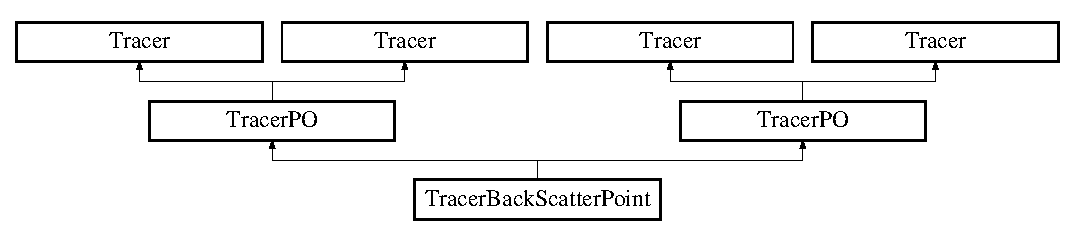
\includegraphics[height=2.727273cm]{class_tracer_back_scatter_point}
\end{center}
\end{figure}
\subsection*{Public Member Functions}
\begin{DoxyCompactItemize}
\item 
\mbox{\Hypertarget{class_tracer_back_scatter_point_a19a45ca1758bc87861b28bec20b9c9eb}\label{class_tracer_back_scatter_point_a19a45ca1758bc87861b28bec20b9c9eb}} 
{\bfseries Tracer\+Back\+Scatter\+Point} (\mbox{\hyperlink{class_particle}{Particle}} $\ast$particle, int refl\+Num, const std\+::string \&result\+File\+Name)
\item 
\mbox{\Hypertarget{class_tracer_back_scatter_point_a2db2b1225db5a2cc6e4e8cd436e49ac9}\label{class_tracer_back_scatter_point_a2db2b1225db5a2cc6e4e8cd436e49ac9}} 
void {\bfseries Trace} (const \mbox{\hyperlink{struct_angle_range}{Angle\+Range}} \&beta\+Range, const \mbox{\hyperlink{struct_angle_range}{Angle\+Range}} \&gamma\+Range, const \mbox{\hyperlink{class_tracks}{Tracks}} \&tracks, double wave)
\item 
\mbox{\Hypertarget{class_tracer_back_scatter_point_a19a45ca1758bc87861b28bec20b9c9eb}\label{class_tracer_back_scatter_point_a19a45ca1758bc87861b28bec20b9c9eb}} 
{\bfseries Tracer\+Back\+Scatter\+Point} (\mbox{\hyperlink{class_particle}{Particle}} $\ast$particle, int refl\+Num, const std\+::string \&result\+File\+Name)
\item 
\mbox{\Hypertarget{class_tracer_back_scatter_point_a2db2b1225db5a2cc6e4e8cd436e49ac9}\label{class_tracer_back_scatter_point_a2db2b1225db5a2cc6e4e8cd436e49ac9}} 
void {\bfseries Trace} (const \mbox{\hyperlink{struct_angle_range}{Angle\+Range}} \&beta\+Range, const \mbox{\hyperlink{struct_angle_range}{Angle\+Range}} \&gamma\+Range, const \mbox{\hyperlink{class_tracks}{Tracks}} \&tracks, double wave)
\end{DoxyCompactItemize}
\subsection*{Additional Inherited Members}


The documentation for this class was generated from the following files\+:\begin{DoxyCompactItemize}
\item 
common/Tracer\+Back\+Scatter\+Point.\+h\item 
common/Tracer\+Back\+Scatter\+Point.\+cpp\end{DoxyCompactItemize}

\hypertarget{class_tracer_g_o}{}\section{Tracer\+GO Class Reference}
\label{class_tracer_g_o}\index{Tracer\+GO@{Tracer\+GO}}


Inheritance diagram for Tracer\+GO\+:
% FIG 0


Collaboration diagram for Tracer\+GO\+:
% FIG 1
\subsection*{Public Member Functions}
\begin{DoxyCompactItemize}
\item 
\mbox{\Hypertarget{class_tracer_g_o_abe9530e32399e92b297868a133787109}\label{class_tracer_g_o_abe9530e32399e92b297868a133787109}} 
{\bfseries Tracer\+GO} (\mbox{\hyperlink{class_particle}{Particle}} $\ast$particle, int max\+Act\+No, const std\+::string \&result\+File\+Name)
\item 
\mbox{\Hypertarget{class_tracer_g_o_a23f4c1a224e17fc620cf7fcef197716f}\label{class_tracer_g_o_a23f4c1a224e17fc620cf7fcef197716f}} 
void {\bfseries Trace\+Random} (const \mbox{\hyperlink{struct_angle_range}{Angle\+Range}} \&beta\+Range, const \mbox{\hyperlink{struct_angle_range}{Angle\+Range}} \&gamma\+Range)
\item 
\mbox{\Hypertarget{class_tracer_g_o_a85ff51763a379abcc4fa84fba1093ef2}\label{class_tracer_g_o_a85ff51763a379abcc4fa84fba1093ef2}} 
void {\bfseries Trace\+Fixed} (const double \&beta, const double \&gamma)
\end{DoxyCompactItemize}
\subsection*{Protected Member Functions}
\begin{DoxyCompactItemize}
\item 
\mbox{\Hypertarget{class_tracer_g_o_a61ff6ee937f176142c83b4273dfc8545}\label{class_tracer_g_o_a61ff6ee937f176142c83b4273dfc8545}} 
double {\bfseries Calc\+Norm} (long long or\+Num)
\item 
\mbox{\Hypertarget{class_tracer_g_o_a716aa00f03bcfc581ce47f8cca60259f}\label{class_tracer_g_o_a716aa00f03bcfc581ce47f8cca60259f}} 
void {\bfseries Output\+Summary} (int or\+Number, double D\+\_\+tot, double N\+RM, \mbox{\hyperlink{class_calc_timer}{Calc\+Timer}} \&timer)
\end{DoxyCompactItemize}
\subsection*{Additional Inherited Members}


The documentation for this class was generated from the following files\+:\begin{DoxyCompactItemize}
\item 
tracer/Tracer\+G\+O.\+h\item 
tracer/Tracer\+G\+O.\+cpp\end{DoxyCompactItemize}

\hypertarget{class_tracer_p_o}{}\section{Tracer\+PO Class Reference}
\label{class_tracer_p_o}\index{Tracer\+PO@{Tracer\+PO}}
Inheritance diagram for Tracer\+PO\+:\begin{figure}[H]
\begin{center}
\leavevmode
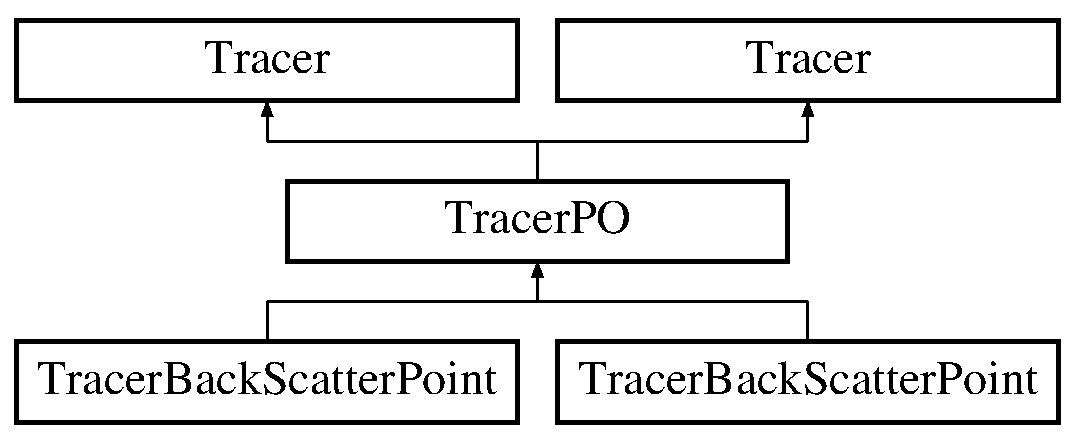
\includegraphics[height=3.000000cm]{class_tracer_p_o}
\end{center}
\end{figure}
\subsection*{Public Member Functions}
\begin{DoxyCompactItemize}
\item 
\mbox{\Hypertarget{class_tracer_p_o_a0868dc6583ce53ecfc54ea4cffcfbb6a}\label{class_tracer_p_o_a0868dc6583ce53ecfc54ea4cffcfbb6a}} 
{\bfseries Tracer\+PO} (\mbox{\hyperlink{class_particle}{Particle}} $\ast$particle, int n\+Acts, const std\+::string \&result\+File\+Name)
\item 
\mbox{\Hypertarget{class_tracer_p_o_a48cbbcf3794ae8b1a2ef4bb3891ba4e8}\label{class_tracer_p_o_a48cbbcf3794ae8b1a2ef4bb3891ba4e8}} 
void {\bfseries Trace\+Random} (const \mbox{\hyperlink{struct_angle_range}{Angle\+Range}} \&beta\+Range, const \mbox{\hyperlink{struct_angle_range}{Angle\+Range}} \&gamma\+Range)
\item 
\mbox{\Hypertarget{class_tracer_p_o_a574b8cd5022759ce5d31c40b334ed395}\label{class_tracer_p_o_a574b8cd5022759ce5d31c40b334ed395}} 
void {\bfseries Trace\+Fixed} (const double \&beta, const double \&gamma)
\item 
\mbox{\Hypertarget{class_tracer_p_o_a0868dc6583ce53ecfc54ea4cffcfbb6a}\label{class_tracer_p_o_a0868dc6583ce53ecfc54ea4cffcfbb6a}} 
{\bfseries Tracer\+PO} (\mbox{\hyperlink{class_particle}{Particle}} $\ast$particle, int n\+Acts, const std\+::string \&result\+File\+Name)
\item 
\mbox{\Hypertarget{class_tracer_p_o_a48cbbcf3794ae8b1a2ef4bb3891ba4e8}\label{class_tracer_p_o_a48cbbcf3794ae8b1a2ef4bb3891ba4e8}} 
void {\bfseries Trace\+Random} (const \mbox{\hyperlink{struct_angle_range}{Angle\+Range}} \&beta\+Range, const \mbox{\hyperlink{struct_angle_range}{Angle\+Range}} \&gamma\+Range)
\item 
\mbox{\Hypertarget{class_tracer_p_o_a574b8cd5022759ce5d31c40b334ed395}\label{class_tracer_p_o_a574b8cd5022759ce5d31c40b334ed395}} 
void {\bfseries Trace\+Fixed} (const double \&beta, const double \&gamma)
\end{DoxyCompactItemize}
\subsection*{Additional Inherited Members}


The documentation for this class was generated from the following files\+:\begin{DoxyCompactItemize}
\item 
common/Tracer\+P\+O.\+h\item 
common/Tracer\+P\+O.\+cpp\end{DoxyCompactItemize}

\hypertarget{class_tracing}{}\section{Tracing Class Reference}
\label{class_tracing}\index{Tracing@{Tracing}}
Inheritance diagram for Tracing\+:\begin{figure}[H]
\begin{center}
\leavevmode
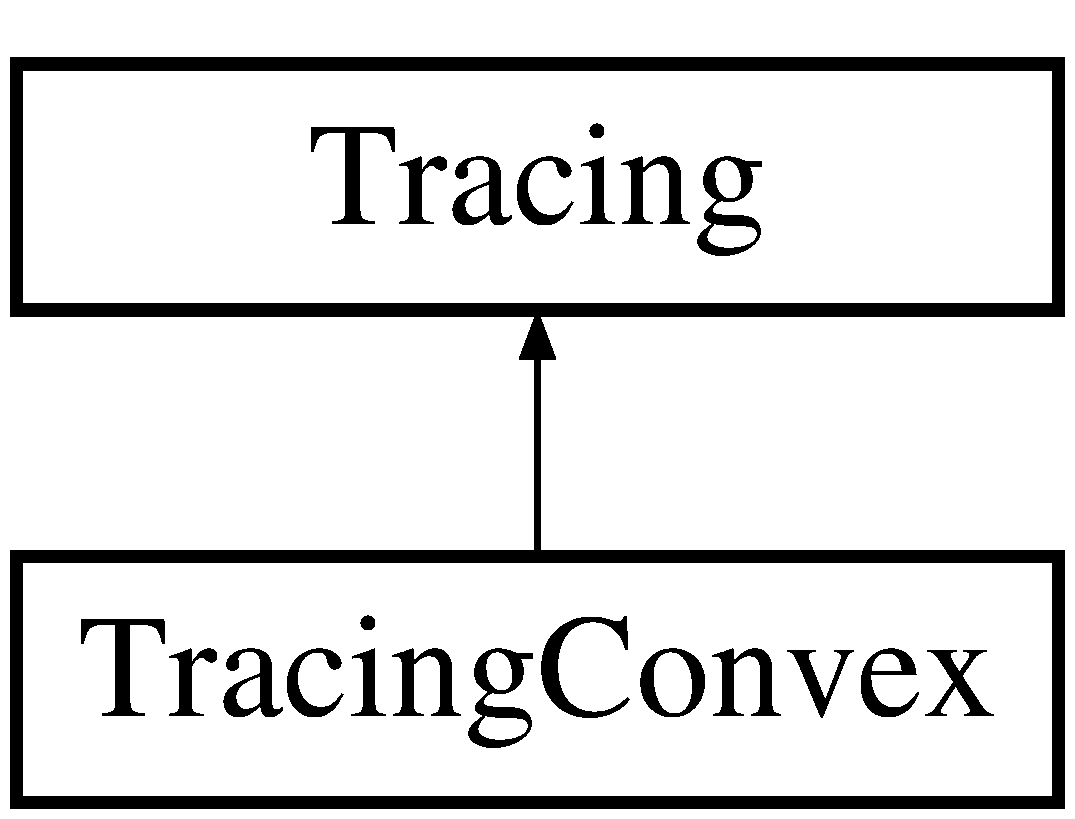
\includegraphics[height=2.000000cm]{class_tracing}
\end{center}
\end{figure}
\subsection*{Public Member Functions}
\begin{DoxyCompactItemize}
\item 
\mbox{\Hypertarget{class_tracing_acd69ed15b6ee7ec09bb032d8d1988ac3}\label{class_tracing_acd69ed15b6ee7ec09bb032d8d1988ac3}} 
{\bfseries Tracing} (\mbox{\hyperlink{class_particle}{Particle}} $\ast$particle, \mbox{\hyperlink{class_light}{Light}} $\ast$incident\+Light, bool is\+Optical\+Path, int inter\+Reflection\+Number)
\item 
\mbox{\Hypertarget{class_tracing_a6bab64b22d0a0821ce687bee1ce134d2}\label{class_tracing_a6bab64b22d0a0821ce687bee1ce134d2}} 
virtual void {\bfseries Split\+Beam\+By\+Particle} (double, double, std\+::vector$<$ \mbox{\hyperlink{class_beam}{Beam}} $>$ \&)
\item 
\mbox{\Hypertarget{class_tracing_acbe2779573da6b926db3ddd79f9d2e91}\label{class_tracing_acbe2779573da6b926db3ddd79f9d2e91}} 
virtual void {\bfseries Split\+Beam\+By\+Particle} (double beta, double gamma, const std\+::vector$<$ std\+::vector$<$ int $>$$>$ \&tracks, std\+::vector$<$ \mbox{\hyperlink{class_beam}{Beam}} $>$ \&scaterred\+Beams)
\item 
\mbox{\Hypertarget{class_tracing_abdc4eaa61b6c1084d6091fe0b5c8496e}\label{class_tracing_abdc4eaa61b6c1084d6091fe0b5c8496e}} 
double {\bfseries Get\+Incoming\+Energy} () const
\item 
\mbox{\Hypertarget{class_tracing_afd7ac36166da74e5f61f96d8373155d2}\label{class_tracing_afd7ac36166da74e5f61f96d8373155d2}} 
double {\bfseries Compute\+Internal\+Optical\+Path} (const \mbox{\hyperlink{class_beam}{Beam}} \&beam, const std\+::vector$<$ int $>$ \&tr)
\end{DoxyCompactItemize}
\subsection*{Public Attributes}
\begin{DoxyCompactItemize}
\item 
\mbox{\Hypertarget{class_tracing_a1efb92d44fd7c64e6a10379ef2d14dbd}\label{class_tracing_a1efb92d44fd7c64e6a10379ef2d14dbd}} 
\mbox{\hyperlink{class_particle}{Particle}} $\ast$ \mbox{\hyperlink{class_tracing_a1efb92d44fd7c64e6a10379ef2d14dbd}{m\+\_\+particle}}
\begin{DoxyCompactList}\small\item\em scattering particle (crystal) \end{DoxyCompactList}\end{DoxyCompactItemize}
\subsection*{Protected Member Functions}
\begin{DoxyCompactItemize}
\item 
\mbox{\Hypertarget{class_tracing_aec003fe5ec76d682820343d140bad9ac}\label{class_tracing_aec003fe5ec76d682820343d140bad9ac}} 
void {\bfseries Set\+Beam\+Optical\+Params} (int facet\+Id, \mbox{\hyperlink{class_beam}{Beam}} \&in\+Beam, \mbox{\hyperlink{class_beam}{Beam}} \&out\+Beam)
\item 
\mbox{\Hypertarget{class_tracing_a978af0f403e8cc7a9bfd356765f9bb48}\label{class_tracing_a978af0f403e8cc7a9bfd356765f9bb48}} 
void {\bfseries Set\+Beam} (\mbox{\hyperlink{class_beam}{Beam}} \&beam, const \mbox{\hyperlink{class_beam}{Beam}} \&other, const \mbox{\hyperlink{struct_point3f}{Point3f}} \&dir, const \mbox{\hyperlink{classcomplex}{complex}} \&coef1, const \mbox{\hyperlink{classcomplex}{complex}} \&coef2) const
\item 
\mbox{\Hypertarget{class_tracing_a99dc46565a81fbedc5bfdcd252e310d3}\label{class_tracing_a99dc46565a81fbedc5bfdcd252e310d3}} 
void {\bfseries Difference} (const \mbox{\hyperlink{class_polygon}{Polygon}} \&subject, const \mbox{\hyperlink{struct_point3f}{Point3f}} \&subj\+Normal, const \mbox{\hyperlink{class_polygon}{Polygon}} \&clip, const \mbox{\hyperlink{struct_point3f}{Point3f}} \&clip\+Normal, const \mbox{\hyperlink{struct_point3f}{Point3f}} \&clip\+Dir, \mbox{\hyperlink{class_polygon}{Polygon}} $\ast$difference, int \&result\+Size) const
\item 
\mbox{\Hypertarget{class_tracing_a257f8200eaf682dac765d100391c5d1e}\label{class_tracing_a257f8200eaf682dac765d100391c5d1e}} 
bool \mbox{\hyperlink{class_tracing_a257f8200eaf682dac765d100391c5d1e}{Intersect}} (int facet\+Id, const \mbox{\hyperlink{class_beam}{Beam}} \&beam, \mbox{\hyperlink{class_polygon}{Polygon}} \&intersection) const
\begin{DoxyCompactList}\small\item\em N\+O\+TE\+: вершины пучка и грани должны быть ориентированы в одном направлении \end{DoxyCompactList}\item 
void \mbox{\hyperlink{class_tracing_a6968bb9a769fc44e191355d70c0cf56e}{Set\+Polygon\+By\+Facet}} (int facet\+Id, \mbox{\hyperlink{class_polygon}{Polygon}} \&polygon) const
\item 
\mbox{\Hypertarget{class_tracing_a8d31b476a030d623e9d2390e97af7028}\label{class_tracing_a8d31b476a030d623e9d2390e97af7028}} 
void {\bfseries Calc\+Optical\+Path} (double cos\+IN, const \mbox{\hyperlink{class_beam}{Beam}} \&incident\+Beam, \mbox{\hyperlink{class_beam}{Beam}} \&in\+Beam, \mbox{\hyperlink{class_beam}{Beam}} \&out\+Beam) const
\item 
\mbox{\Hypertarget{class_tracing_a4ea27d6eac331e809307fcbb0acaf822}\label{class_tracing_a4ea27d6eac331e809307fcbb0acaf822}} 
bool {\bfseries Is\+Terminal\+Beam} (const \mbox{\hyperlink{class_beam}{Beam}} \&beam)
\item 
\mbox{\Hypertarget{class_tracing_a2d192e0a23637161bcd7e49a60f12acc}\label{class_tracing_a2d192e0a23637161bcd7e49a60f12acc}} 
void {\bfseries Trace\+First\+Beam} (int facet\+Id, \mbox{\hyperlink{class_beam}{Beam}} \&in\+Beam, \mbox{\hyperlink{class_beam}{Beam}} \&out\+Beam)
\item 
void \mbox{\hyperlink{class_tracing_a1eb24906dd1db23bdffbdfc4d7864baf}{Trace\+Secondary\+Beams}} (\mbox{\hyperlink{class_beam}{Beam}} \&incident\+Beam, int facet\+ID, \mbox{\hyperlink{class_beam}{Beam}} \&in\+Beam, std\+::vector$<$ \mbox{\hyperlink{class_beam}{Beam}} $>$ \&out\+Beams)
\item 
\mbox{\Hypertarget{class_tracing_a9cc5f8b35b0f3e5791ca62cb10e598e4}\label{class_tracing_a9cc5f8b35b0f3e5791ca62cb10e598e4}} 
void {\bfseries Rotate\+Polarisation\+Plane} (const \mbox{\hyperlink{struct_point3f}{Point3f}} \&dir, const \mbox{\hyperlink{struct_point3f}{Point3f}} \&facet\+Normal, \mbox{\hyperlink{class_beam}{Beam}} \&beam)
\item 
\mbox{\Hypertarget{class_tracing_a25e87ab96197e6e13ba206c721305dee}\label{class_tracing_a25e87ab96197e6e13ba206c721305dee}} 
void {\bfseries Set\+Slopping\+Beam\+Params\+\_\+initial} (const \mbox{\hyperlink{struct_point3f}{Point3f}} \&beam\+Dir, double cos\+IN, int facet\+Id, \mbox{\hyperlink{class_beam}{Beam}} \&in\+Beam, \mbox{\hyperlink{class_beam}{Beam}} \&out\+Beam)
\item 
\mbox{\Hypertarget{class_tracing_a2520c8204b764df82682b7ba7655559f}\label{class_tracing_a2520c8204b764df82682b7ba7655559f}} 
void {\bfseries Set\+Normal\+Incidence\+Beam\+Params} (double cos\+IN, const \mbox{\hyperlink{class_beam}{Beam}} \&incident\+Beam, \mbox{\hyperlink{class_beam}{Beam}} \&in\+Beam, \mbox{\hyperlink{class_beam}{Beam}} \&out\+Beam)
\item 
void \mbox{\hyperlink{class_tracing_a426d2564586b18910ddd7407fcc5fd47}{Set\+Slopping\+Incidence\+Beam\+Params}} (double cos\+IN, const \mbox{\hyperlink{struct_point3f}{Point3f}} \&normal, \mbox{\hyperlink{class_beam}{Beam}} \&incident\+Beam, \mbox{\hyperlink{class_beam}{Beam}} \&in\+Beam, \mbox{\hyperlink{class_beam}{Beam}} \&out\+Beam, bool \&is\+Trivial\+Incidence)
\item 
\mbox{\Hypertarget{class_tracing_a1eca7de1606439f44b85e6bc03e4f09e}\label{class_tracing_a1eca7de1606439f44b85e6bc03e4f09e}} 
void {\bfseries Calc\+Facet\+Energy} (int facet\+ID, const \mbox{\hyperlink{class_polygon}{Polygon}} \&lighted\+Polygon)
\item 
\mbox{\Hypertarget{class_tracing_a05ee4083d55c4ed73f59ea5a9b90df61}\label{class_tracing_a05ee4083d55c4ed73f59ea5a9b90df61}} 
void {\bfseries Calc\+Optical\+Path\+\_\+initial} (\mbox{\hyperlink{class_beam}{Beam}} \&in\+Beam, \mbox{\hyperlink{class_beam}{Beam}} \&out\+Beam)
\item 
\mbox{\Hypertarget{class_tracing_a2d3d2ac9923c515398381ef2a269e579}\label{class_tracing_a2d3d2ac9923c515398381ef2a269e579}} 
void {\bfseries Push\+Beam\+To\+Tree} (\mbox{\hyperlink{class_beam}{Beam}} \&beam, int facet\+Id, int level, Location location)
\item 
\mbox{\Hypertarget{class_tracing_a43f4c6c8b6641a5bfa009e6805d66e9d}\label{class_tracing_a43f4c6c8b6641a5bfa009e6805d66e9d}} 
void {\bfseries Push\+Beam\+To\+Tree} (\mbox{\hyperlink{class_beam}{Beam}} \&beam, int facet\+Id, int level)
\item 
\mbox{\Hypertarget{class_tracing_ae29bbd14ab8e082325839b55c68115a8}\label{class_tracing_ae29bbd14ab8e082325839b55c68115a8}} 
void {\bfseries Push\+Beam\+To\+Tree} (\mbox{\hyperlink{class_beam}{Beam}} \&beam)
\item 
\mbox{\Hypertarget{class_tracing_a1578036bb682b4d769c8baf4df6ad65d}\label{class_tracing_a1578036bb682b4d769c8baf4df6ad65d}} 
void {\bfseries Set\+Beam\+ID} (\mbox{\hyperlink{class_beam}{Beam}} \&beam)
\end{DoxyCompactItemize}
\subsection*{Protected Attributes}
\begin{DoxyCompactItemize}
\item 
\mbox{\Hypertarget{class_tracing_ac8f3377fa73be91dfdb166babed6255e}\label{class_tracing_ac8f3377fa73be91dfdb166babed6255e}} 
\mbox{\hyperlink{class_facet}{Facet}} $\ast$ {\bfseries m\+\_\+facets}
\item 
\mbox{\Hypertarget{class_tracing_a7dd12cbc4e59f2ba8b12ddd4b7aed76e}\label{class_tracing_a7dd12cbc4e59f2ba8b12ddd4b7aed76e}} 
\mbox{\hyperlink{class_light}{Light}} $\ast$ {\bfseries m\+\_\+incident\+Light}
\item 
\mbox{\Hypertarget{class_tracing_aefe49bf5c3bffd54cddb2e0acb028f57}\label{class_tracing_aefe49bf5c3bffd54cddb2e0acb028f57}} 
\mbox{\hyperlink{struct_point3f}{Point3f}} {\bfseries m\+\_\+incident\+Dir}
\item 
\mbox{\Hypertarget{class_tracing_aa3e14498c747ce375a67141152f99e10}\label{class_tracing_aa3e14498c747ce375a67141152f99e10}} 
\mbox{\hyperlink{struct_point3f}{Point3f}} {\bfseries m\+\_\+polar\+Basis}
\item 
\mbox{\Hypertarget{class_tracing_a26bb838f98169f69219761999f766ca9}\label{class_tracing_a26bb838f98169f69219761999f766ca9}} 
bool {\bfseries m\+\_\+is\+Optical\+Path}
\item 
\mbox{\Hypertarget{class_tracing_a4daab6ec5b297894faa48b9967d0bd4c}\label{class_tracing_a4daab6ec5b297894faa48b9967d0bd4c}} 
int {\bfseries m\+\_\+inter\+Reflection\+Number}
\item 
\mbox{\Hypertarget{class_tracing_ae147e97b0754d62db2ac62fd36be2046}\label{class_tracing_ae147e97b0754d62db2ac62fd36be2046}} 
\mbox{\hyperlink{class_beam}{Beam}} \mbox{\hyperlink{class_tracing_ae147e97b0754d62db2ac62fd36be2046}{m\+\_\+beam\+Tree}} \mbox{[}M\+A\+X\+\_\+\+B\+E\+A\+M\+\_\+\+R\+E\+F\+L\+\_\+\+N\+UM\mbox{]}
\begin{DoxyCompactList}\small\item\em tree of beams (works like stack) \end{DoxyCompactList}\item 
\mbox{\Hypertarget{class_tracing_a92128489e2b53ece6da4cb069c7bcbbd}\label{class_tracing_a92128489e2b53ece6da4cb069c7bcbbd}} 
int {\bfseries m\+\_\+tree\+Size}
\item 
\mbox{\Hypertarget{class_tracing_a2bd7b2c3a83b1db6ccfee67425f88bca}\label{class_tracing_a2bd7b2c3a83b1db6ccfee67425f88bca}} 
double {\bfseries m\+\_\+incomming\+Energy}
\item 
\mbox{\Hypertarget{class_tracing_afb5d56155efe0b3b97a4663da3b48c0c}\label{class_tracing_afb5d56155efe0b3b97a4663da3b48c0c}} 
const double {\bfseries F\+A\+R\+\_\+\+Z\+O\+N\+E\+\_\+\+D\+I\+S\+T\+A\+N\+CE} = 10000.\+0
\item 
\mbox{\Hypertarget{class_tracing_a2a957ec62acbabc7d1f1926bf75a00ff}\label{class_tracing_a2a957ec62acbabc7d1f1926bf75a00ff}} 
const double {\bfseries E\+P\+S\+\_\+\+B\+E\+A\+M\+\_\+\+E\+N\+E\+R\+GY} = 2e-\/12
\end{DoxyCompactItemize}


\subsection{Member Function Documentation}
\mbox{\Hypertarget{class_tracing_a6968bb9a769fc44e191355d70c0cf56e}\label{class_tracing_a6968bb9a769fc44e191355d70c0cf56e}} 
\index{Tracing@{Tracing}!Set\+Polygon\+By\+Facet@{Set\+Polygon\+By\+Facet}}
\index{Set\+Polygon\+By\+Facet@{Set\+Polygon\+By\+Facet}!Tracing@{Tracing}}
\subsubsection{\texorpdfstring{Set\+Polygon\+By\+Facet()}{SetPolygonByFacet()}}
{\footnotesize\ttfamily void Tracing\+::\+Set\+Polygon\+By\+Facet (\begin{DoxyParamCaption}\item[{int}]{facet\+Id,  }\item[{\mbox{\hyperlink{class_polygon}{Polygon}} \&}]{polygon }\end{DoxyParamCaption}) const\hspace{0.3cm}{\ttfamily [protected]}}

N\+O\+TE\+: Result beams are ordered in inverse direction \mbox{\Hypertarget{class_tracing_a426d2564586b18910ddd7407fcc5fd47}\label{class_tracing_a426d2564586b18910ddd7407fcc5fd47}} 
\index{Tracing@{Tracing}!Set\+Slopping\+Incidence\+Beam\+Params@{Set\+Slopping\+Incidence\+Beam\+Params}}
\index{Set\+Slopping\+Incidence\+Beam\+Params@{Set\+Slopping\+Incidence\+Beam\+Params}!Tracing@{Tracing}}
\subsubsection{\texorpdfstring{Set\+Slopping\+Incidence\+Beam\+Params()}{SetSloppingIncidenceBeamParams()}}
{\footnotesize\ttfamily void Tracing\+::\+Set\+Slopping\+Incidence\+Beam\+Params (\begin{DoxyParamCaption}\item[{double}]{cos\+IN,  }\item[{const \mbox{\hyperlink{struct_point3f}{Point3f}} \&}]{normal,  }\item[{\mbox{\hyperlink{class_beam}{Beam}} \&}]{incident\+Beam,  }\item[{\mbox{\hyperlink{class_beam}{Beam}} \&}]{in\+Beam,  }\item[{\mbox{\hyperlink{class_beam}{Beam}} \&}]{out\+Beam,  }\item[{bool \&}]{is\+Trivial\+Incidence }\end{DoxyParamCaption})\hspace{0.3cm}{\ttfamily [protected]}}

trivial incidence

complete internal reflection \mbox{\Hypertarget{class_tracing_a1eb24906dd1db23bdffbdfc4d7864baf}\label{class_tracing_a1eb24906dd1db23bdffbdfc4d7864baf}} 
\index{Tracing@{Tracing}!Trace\+Secondary\+Beams@{Trace\+Secondary\+Beams}}
\index{Trace\+Secondary\+Beams@{Trace\+Secondary\+Beams}!Tracing@{Tracing}}
\subsubsection{\texorpdfstring{Trace\+Secondary\+Beams()}{TraceSecondaryBeams()}}
{\footnotesize\ttfamily void Tracing\+::\+Trace\+Secondary\+Beams (\begin{DoxyParamCaption}\item[{\mbox{\hyperlink{class_beam}{Beam}} \&}]{incident\+Beam,  }\item[{int}]{facet\+ID,  }\item[{\mbox{\hyperlink{class_beam}{Beam}} \&}]{in\+Beam,  }\item[{std\+::vector$<$ \mbox{\hyperlink{class_beam}{Beam}} $>$ \&}]{out\+Beams }\end{DoxyParamCaption})\hspace{0.3cm}{\ttfamily [protected]}}

beam is not incident to this facet

normal incidence

slopping incidence 

The documentation for this class was generated from the following files\+:\begin{DoxyCompactItemize}
\item 
tracing/Tracing.\+h\item 
tracing/Tracing.\+cpp\end{DoxyCompactItemize}

\hypertarget{class_tracing_convex}{}\section{Tracing\+Convex Class Reference}
\label{class_tracing_convex}\index{Tracing\+Convex@{Tracing\+Convex}}
Inheritance diagram for Tracing\+Convex\+:\begin{figure}[H]
\begin{center}
\leavevmode
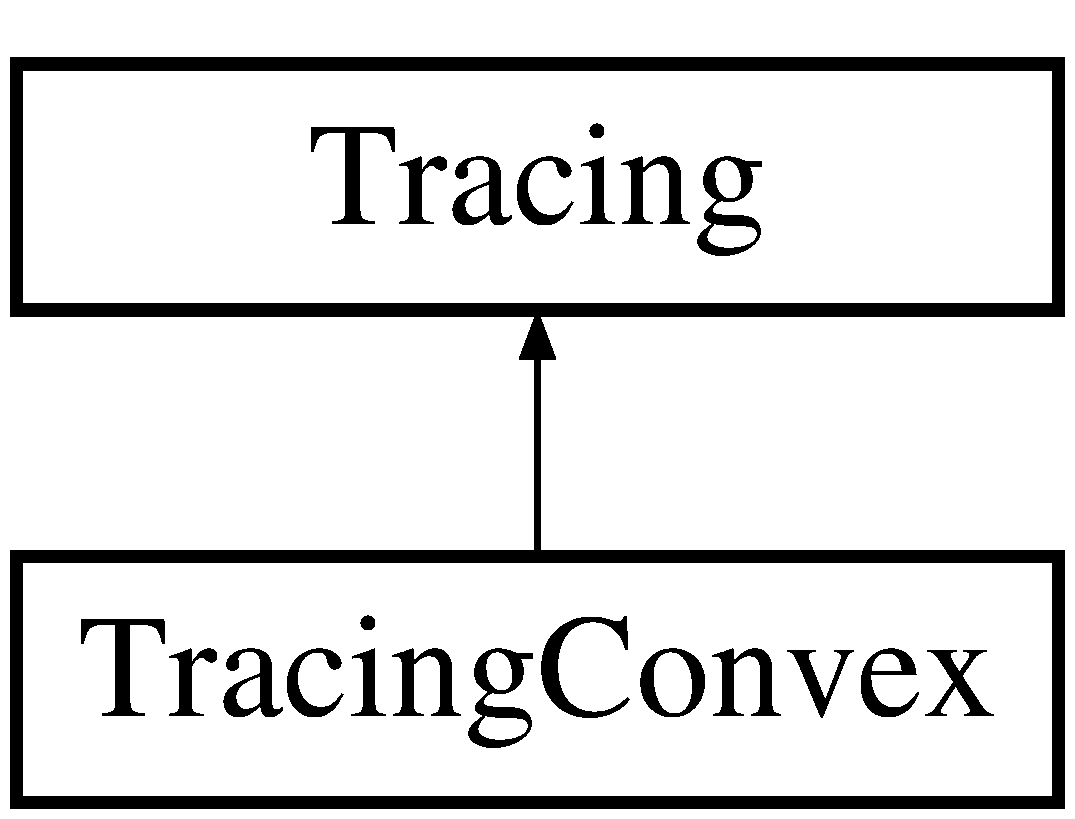
\includegraphics[height=2.000000cm]{class_tracing_convex}
\end{center}
\end{figure}
\subsection*{Public Member Functions}
\begin{DoxyCompactItemize}
\item 
\mbox{\Hypertarget{class_tracing_convex_af740406e6033d8546b57ff144231d79d}\label{class_tracing_convex_af740406e6033d8546b57ff144231d79d}} 
{\bfseries Tracing\+Convex} (\mbox{\hyperlink{class_particle}{Particle}} $\ast$particle, \mbox{\hyperlink{class_light}{Light}} $\ast$incident\+Light, bool is\+Optical\+Path, int inter\+Reflection\+Number)
\item 
void \mbox{\hyperlink{class_tracing_convex_a6af4ffe46712b46b5472a7d7c930fb04}{Split\+Beam\+By\+Particle}} (double beta, double gamma, std\+::vector$<$ \mbox{\hyperlink{class_beam}{Beam}} $>$ \&out\+Beams) override
\item 
\mbox{\Hypertarget{class_tracing_convex_a67d185bea9fed4c2500496495659fc2b}\label{class_tracing_convex_a67d185bea9fed4c2500496495659fc2b}} 
void {\bfseries Split\+Beam\+By\+Particle} (double, double, const std\+::vector$<$ std\+::vector$<$ int $>$$>$ \&, std\+::vector$<$ \mbox{\hyperlink{class_beam}{Beam}} $>$ \&) override
\end{DoxyCompactItemize}
\subsection*{Protected Member Functions}
\begin{DoxyCompactItemize}
\item 
\mbox{\Hypertarget{class_tracing_convex_a089c68d6a92e53aa7a1741586c46ee3c}\label{class_tracing_convex_a089c68d6a92e53aa7a1741586c46ee3c}} 
void \mbox{\hyperlink{class_tracing_convex_a089c68d6a92e53aa7a1741586c46ee3c}{Trace\+Internal\+Beams}} (std\+::vector$<$ \mbox{\hyperlink{class_beam}{Beam}} $>$ \&out\+Beams)
\begin{DoxyCompactList}\small\item\em \begin{quote}
for predefined trajectories \end{quote}
\end{DoxyCompactList}\end{DoxyCompactItemize}
\subsection*{Additional Inherited Members}


\subsection{Member Function Documentation}
\mbox{\Hypertarget{class_tracing_convex_a6af4ffe46712b46b5472a7d7c930fb04}\label{class_tracing_convex_a6af4ffe46712b46b5472a7d7c930fb04}} 
\index{Tracing\+Convex@{Tracing\+Convex}!Split\+Beam\+By\+Particle@{Split\+Beam\+By\+Particle}}
\index{Split\+Beam\+By\+Particle@{Split\+Beam\+By\+Particle}!Tracing\+Convex@{Tracing\+Convex}}
\subsubsection{\texorpdfstring{Split\+Beam\+By\+Particle()}{SplitBeamByParticle()}}
{\footnotesize\ttfamily void Tracing\+Convex\+::\+Split\+Beam\+By\+Particle (\begin{DoxyParamCaption}\item[{double}]{beta,  }\item[{double}]{gamma,  }\item[{std\+::vector$<$ \mbox{\hyperlink{class_beam}{Beam}} $>$ \&}]{out\+Beams }\end{DoxyParamCaption})\hspace{0.3cm}{\ttfamily [override]}, {\ttfamily [virtual]}}

first extermal beam

beam is not incident to this facet 

Reimplemented from \mbox{\hyperlink{class_tracing}{Tracing}}.



The documentation for this class was generated from the following files\+:\begin{DoxyCompactItemize}
\item 
tracing/Tracing\+Convex.\+h\item 
tracing/Tracing\+Convex.\+cpp\end{DoxyCompactItemize}

\hypertarget{class_track}{}\section{Track Class Reference}
\label{class_track}\index{Track@{Track}}


Inheritance diagram for Track\+:
% FIG 0


Collaboration diagram for Track\+:
% FIG 1
\subsection*{Public Member Functions}
\begin{DoxyCompactItemize}
\item 
\mbox{\Hypertarget{class_track_a4df6f946922339d5f9f64d4b6a0ce27c}\label{class_track_a4df6f946922339d5f9f64d4b6a0ce27c}} 
void {\bfseries Update} (\mbox{\hyperlink{class_facet}{Facet}} $\ast$face)
\item 
bool \mbox{\hyperlink{class_track_afa8ecb5618ed9ecefab2ea5f0e755d44}{Is\+Inside\+On\+Act}} (int i\+Act) const
\begin{DoxyCompactList}\small\item\em Shows where the \mbox{\hyperlink{class_beam}{Beam}} is located towards the \mbox{\hyperlink{class_particle}{Particle}} inside or outside. \end{DoxyCompactList}\item 
\mbox{\Hypertarget{class_track_aa9152f9a092de15ac7e92cf7120222eb}\label{class_track_aa9152f9a092de15ac7e92cf7120222eb}} 
void {\bfseries Recompute\+Track\+Id} (int facet\+Id, int n\+Facets)
\item 
\mbox{\Hypertarget{class_track_a5c9b01364289589a2dfaf4a865a88cf1}\label{class_track_a5c9b01364289589a2dfaf4a865a88cf1}} 
\mbox{\hyperlink{class_track}{Track}} \& {\bfseries operator=} (const \mbox{\hyperlink{class_track}{Track}} \&other)
\end{DoxyCompactItemize}
\subsection*{Public Attributes}
\begin{DoxyCompactItemize}
\item 
\mbox{\Hypertarget{class_track_a04d6f364003aa9e8cd212df0dbb2447f}\label{class_track_a04d6f364003aa9e8cd212df0dbb2447f}} 
\mbox{\hyperlink{class_big_integer}{Id\+Type}} \mbox{\hyperlink{class_track_a04d6f364003aa9e8cd212df0dbb2447f}{id}}
\begin{DoxyCompactList}\small\item\em Unique id of beam calculated by facet ids. \end{DoxyCompactList}\item 
int \mbox{\hyperlink{class_track_a9a1bcdb52e5765ac6d91e62f26a51df0}{locations}}
\item 
\mbox{\Hypertarget{class_track_a677ef64963f95925017853f2657722c7}\label{class_track_a677ef64963f95925017853f2657722c7}} 
int \mbox{\hyperlink{class_track_a677ef64963f95925017853f2657722c7}{act\+No}}
\begin{DoxyCompactList}\small\item\em Current r/r act number. \end{DoxyCompactList}\item 
\mbox{\Hypertarget{class_track_aa5529af7dae62559eb396deca64db430}\label{class_track_aa5529af7dae62559eb396deca64db430}} 
\mbox{\hyperlink{class_facet}{Facet}} $\ast$ \mbox{\hyperlink{class_track_aa5529af7dae62559eb396deca64db430}{facet}}
\begin{DoxyCompactList}\small\item\em Last incident facet of the \mbox{\hyperlink{class_particle}{Particle}}. \end{DoxyCompactList}\end{DoxyCompactItemize}


\subsection{Member Function Documentation}
\mbox{\Hypertarget{class_track_afa8ecb5618ed9ecefab2ea5f0e755d44}\label{class_track_afa8ecb5618ed9ecefab2ea5f0e755d44}} 
\index{Track@{Track}!Is\+Inside\+On\+Act@{Is\+Inside\+On\+Act}}
\index{Is\+Inside\+On\+Act@{Is\+Inside\+On\+Act}!Track@{Track}}
\subsubsection{\texorpdfstring{Is\+Inside\+On\+Act()}{IsInsideOnAct()}}
{\footnotesize\ttfamily bool Track\+::\+Is\+Inside\+On\+Act (\begin{DoxyParamCaption}\item[{int}]{i\+Act }\end{DoxyParamCaption}) const\hspace{0.3cm}{\ttfamily [inline]}}



Shows where the \mbox{\hyperlink{class_beam}{Beam}} is located towards the \mbox{\hyperlink{class_particle}{Particle}} inside or outside. 


\begin{DoxyParams}{Parameters}
{\em i\+Act} & r/r act number \\
\hline
\end{DoxyParams}
\begin{DoxyReturn}{Returns}
true if beam location is \char`\"{}inside\char`\"{} on r/r act, otherwise returns false 
\end{DoxyReturn}


\subsection{Member Data Documentation}
\mbox{\Hypertarget{class_track_a9a1bcdb52e5765ac6d91e62f26a51df0}\label{class_track_a9a1bcdb52e5765ac6d91e62f26a51df0}} 
\index{Track@{Track}!locations@{locations}}
\index{locations@{locations}!Track@{Track}}
\subsubsection{\texorpdfstring{locations}{locations}}
{\footnotesize\ttfamily int Track\+::locations}

Every bit of the variable represents location of beam after an r/r act from the right to the left \char`\"{}0\char`\"{} when beam location is \char`\"{}inside\char`\"{} and \char`\"{}1\char`\"{} if it\textquotesingle{}s \char`\"{}outside\char`\"{} 

The documentation for this class was generated from the following file\+:\begin{DoxyCompactItemize}
\item 
common/Beam.\+h\end{DoxyCompactItemize}

\hypertarget{class_track_group}{}\section{Track\+Group Class Reference}
\label{class_track_group}\index{Track\+Group@{Track\+Group}}


{\ttfamily \#include $<$Tracks.\+h$>$}



Collaboration diagram for Track\+Group\+:
% FIG 0
\subsection*{Public Member Functions}
\begin{DoxyCompactItemize}
\item 
\mbox{\Hypertarget{class_track_group_a293ba3cf81474c79045986fd312ef02c}\label{class_track_group_a293ba3cf81474c79045986fd312ef02c}} 
std\+::string {\bfseries Create\+Group\+Name} () const
\end{DoxyCompactItemize}
\subsection*{Public Attributes}
\begin{DoxyCompactItemize}
\item 
\mbox{\Hypertarget{class_track_group_a2a58c0b4da7f12c44a21ad23801b40b3}\label{class_track_group_a2a58c0b4da7f12c44a21ad23801b40b3}} 
int {\bfseries group\+ID}
\item 
\mbox{\Hypertarget{class_track_group_a666a8f118167e57dd4456be90858956a}\label{class_track_group_a666a8f118167e57dd4456be90858956a}} 
\mbox{\hyperlink{class_big_integer}{Id\+Type}} {\bfseries arr} \mbox{[}M\+A\+X\+\_\+\+G\+R\+O\+U\+P\+\_\+\+N\+UM\mbox{]}
\item 
\mbox{\Hypertarget{class_track_group_a339ec7ee74e2c37e860bc4a93e2429b5}\label{class_track_group_a339ec7ee74e2c37e860bc4a93e2429b5}} 
int {\bfseries size} = 0
\item 
\mbox{\Hypertarget{class_track_group_a2e9d60678b059b15c43ee2274fb10d07}\label{class_track_group_a2e9d60678b059b15c43ee2274fb10d07}} 
std\+::vector$<$ std\+::vector$<$ int $>$ $>$ {\bfseries tracks}
\end{DoxyCompactItemize}


\subsection{Detailed Description}
R\+EF O\+PT T\+O\+DO\+: сохранять треки вместе в id в виде массива интов, чтобы не конвертировать, а просто искать их по id 

The documentation for this class was generated from the following file\+:\begin{DoxyCompactItemize}
\item 
tracer/Tracks.\+h\end{DoxyCompactItemize}

\hypertarget{class_tracks}{}\section{Tracks Class Reference}
\label{class_tracks}\index{Tracks@{Tracks}}
Inheritance diagram for Tracks\+:\begin{figure}[H]
\begin{center}
\leavevmode
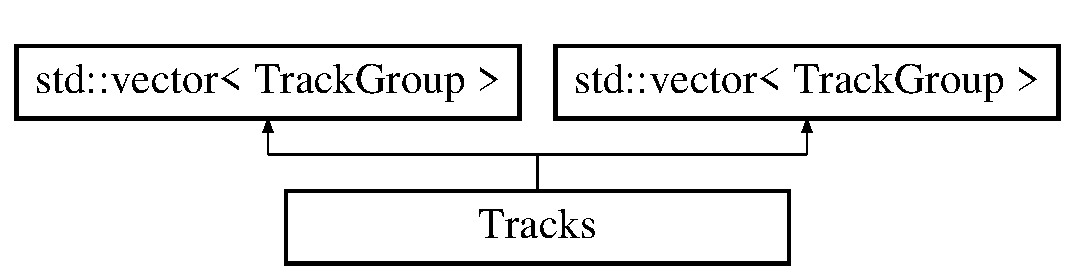
\includegraphics[height=2.000000cm]{class_tracks}
\end{center}
\end{figure}
\subsection*{Public Member Functions}
\begin{DoxyCompactItemize}
\item 
\mbox{\Hypertarget{class_tracks_a1b25ede933c3cae43d01cdf5d16eae54}\label{class_tracks_a1b25ede933c3cae43d01cdf5d16eae54}} 
{\bfseries Tracks} (int n\+Facets)
\item 
\mbox{\Hypertarget{class_tracks_aeee2af5000d0c418f51a33f96d1e93f7}\label{class_tracks_aeee2af5000d0c418f51a33f96d1e93f7}} 
int {\bfseries Find\+Group\+By\+Track\+Id} (const \mbox{\hyperlink{class_big_integer}{Id\+Type}} \&track\+Id) const
\item 
\mbox{\Hypertarget{class_tracks_a7a61b8c7b50c6132a06b9883bf779f1b}\label{class_tracks_a7a61b8c7b50c6132a06b9883bf779f1b}} 
void {\bfseries Import\+Tracks} (int n\+Facets, const std\+::string \&filename)
\item 
\mbox{\Hypertarget{class_tracks_aed07786d2b9af54a341ca8322d39d91c}\label{class_tracks_aed07786d2b9af54a341ca8322d39d91c}} 
void {\bfseries Recover\+Track} (const \mbox{\hyperlink{class_beam}{Beam}} \&beam, std\+::vector$<$ int $>$ \&track)
\item 
\mbox{\Hypertarget{class_tracks_a71e296927bcac5f60bff87c37c71e1db}\label{class_tracks_a71e296927bcac5f60bff87c37c71e1db}} 
int {\bfseries Find\+Group} (const long long \&track\+ID) const
\end{DoxyCompactItemize}
\subsection*{Static Public Member Functions}
\begin{DoxyCompactItemize}
\item 
\mbox{\Hypertarget{class_tracks_aaf66ef556b4523971ccebe04a28d7f7b}\label{class_tracks_aaf66ef556b4523971ccebe04a28d7f7b}} 
static std\+::string {\bfseries Track\+To\+Str} (const std\+::vector$<$ int $>$ \&track)
\item 
\mbox{\Hypertarget{class_tracks_a122cf0fd15ee1c23e58a01d483974985}\label{class_tracks_a122cf0fd15ee1c23e58a01d483974985}} 
static void {\bfseries Recover\+Track} (const \mbox{\hyperlink{class_beam}{Beam}} \&beam, int facet\+Num, std\+::vector$<$ int $>$ \&track)
\end{DoxyCompactItemize}
\subsection*{Public Attributes}
\begin{DoxyCompactItemize}
\item 
\mbox{\Hypertarget{class_tracks_a66cb4ec9a2db84d0abecb7ea327dffdd}\label{class_tracks_a66cb4ec9a2db84d0abecb7ea327dffdd}} 
bool {\bfseries should\+Compute\+Tracks\+Only}
\end{DoxyCompactItemize}


The documentation for this class was generated from the following files\+:\begin{DoxyCompactItemize}
\item 
common/Tracks.\+h\item 
tracing/Tracing.\+h\item 
common/Tracks.\+cpp\end{DoxyCompactItemize}

%--- End generated contents ---

% Index
\backmatter
\newpage
\phantomsection
\clearemptydoublepage
\addcontentsline{toc}{chapter}{Index}
\printindex

\end{document}
